\documentclass[12pt,american,english,notitlepage]{article}

\usepackage{cochineal}
\renewcommand{\familydefault}{\rmdefault}
\usepackage[T1]{fontenc}
%\usepackage[latin9]{inputenc}
\usepackage[active]{srcltx}
\usepackage{float}
\usepackage{amsmath}
\usepackage{amsthm}
\usepackage{amssymb}
\usepackage{graphicx}
\usepackage{geometry}
\geometry{verbose,tmargin=1.in,bmargin=1.in,lmargin=1in,rmargin=1in}
\usepackage{setspace}
\usepackage[authoryear,longnamesfirst]{natbib}

\usepackage{pdflscape}
\usepackage{placeins}


\onehalfspacing

\makeatletter

%%%%%%%%%%%%%%%%%%%%%%%%%%%%%% LyX specific LaTeX commands.
%% Because html converters don't know tabularnewline
\providecommand{\tabularnewline}{\\}

%%%%%%%%%%%%%%%%%%%%%%%%%%%%%% Textclass specific LaTeX commands.
\theoremstyle{plain}
\newtheorem{cor}{\protect\corollaryname}
\newenvironment{lyxlist}[1]
	{\begin{list}{}
		{\settowidth{\labelwidth}{#1}
		 \setlength{\leftmargin}{\labelwidth}
		 \addtolength{\leftmargin}{\labelsep}
		 \renewcommand{\makelabel}[1]{##1\hfil}}}
	{\end{list}}

%%%%%%%%%%%%%%%%%%%%%%%%%%%%%% User specified LaTeX commands.
\special{papersize=8.5in,11in}
%\usepackage{palatino,amssymb,amsfonts,amsmath,latexsym,setspace}
\usepackage{amsfonts}
\usepackage{latexsym}
% \usepackage[dvips]{graphicx}
\usepackage{amsmath}
\usepackage{fancyhdr}

%%%%%%%%%%%%%%%%%%%%%%%%%%%%%%%%%%%%%%%%%%%%%%%%%%%%%%%%%%%%%%%%%%%%%%%%%%%%%%%%%%%%%%%%%%%%%%%%%%%%%%%%%%%%%%%%%%%%%%%%%%%%%%%%%%%%%%%%%%%%%%%%%%%%%%%%%%%%%%%%%%%%%%%%%%%%%%%%%%%%%%%%%%%%%%%%%%%%%%%%%%%%%%%%%%%%%%%%%%%%%%%%%%%%%%%%%%%%%%%%%%%%%%%%%%%%
\usepackage{amsfonts}
\usepackage{array}
\usepackage{lscape}
% \usepackage{color}

\usepackage{colortbl}
 \usepackage{xcolor}
\usepackage{caption}
\usepackage{subfig}
% \usepackage{subcaption}
\usepackage{sidecap}

\usepackage{tikz,pgf}
\usetikzlibrary{decorations.text}
\usetikzlibrary{patterns}
\usepackage{pgfplots}
% \pgfplotsset{compat=1.18}
\usepackage{verbatim}
\usepackage{algorithm}
\usepackage{algorithmic}

% \usepackage[longnamesfirst]{natbib}
\bibliographystyle{aer}

\usepackage{hyperref}
\hypersetup{breaklinks = true,
colorlinks=true, anchorcolor= ChadBlue, citecolor= ChadBlue,
filecolor= ChadBlue, linkcolor= ChadBlue, menucolor= ChadBlue,
urlcolor= blue, citebordercolor= 1 0 0, menubordercolor=1 0
0, urlbordercolor=1 0 0, runbordercolor=1 0 0 }


\setcounter{MaxMatrixCols}{10}
%  Chad's style file for nice paper format.
%  Various ideas for this style are taken from
%    -- Matthias Doepke and Michele Tertilt
%    -- Tony Roberts


% example file to change the style of LaTeX
% first colour for latex or pdflatex
%\ifx\pdfoutput\@undefined\usepackage[usenames,dvips]{color}
% \else\usepackage[usenames,dvipsnames]{color}
% and fix pdf colour problems
% \IfFileExists{pdfcolmk.sty}{\usepackage{pdfcolmk}}{} 
%\fi

% Chad's colors:
% See http://web.njit.edu/~kevin/rgb.txt.html for possibilities
\definecolor{ChadDarkBlue}{rgb}{.1,0,.2}  
\definecolor{ChadBlue}{rgb}{.1,.1,.5}  
\definecolor{ChadRoyal}{rgb}{.2,.2,.8}  
%\definecolor{ChadGreen}{rgb}{0,.35,.1}
%\definecolor{ChadGreen}{rgb}{0,.5,.25}  % Too bright
%\definecolor{ChadGreen}{rgb}{0,.4,.2}    % Still too bright
\definecolor{ChadGreen}{rgb}{0,.4,0}    % Dark Green
%\definecolor{ChadRed}{rgb}{.8,.1,.2}    % Too bright
\definecolor{ChadRed}{rgb}{.5,0,.5}  % purple
\definecolor{ChadMagenta}{rgb}{.6,0,.6}  % magenta
\definecolor{webbrown}{rgb}{.1,0,.2}  % magenta

%%% HYPERLINKS %%%%%%%%%%%%%%%%%%%%%
\usepackage[figure,table]{hypcap}% Correct a problem with hyperref
\urlstyle{rm} %so it doesn't use a typewriter font for url's.

% Hyperstuff
% \hypersetup{citecolor=webbrown,linkcolor=ChadDarkBlue,urlcolor=ChadDarkBlue}


%%%%%%%%%%%%%%%%%%%%%


% Fix title, sections, etc.

\let\LaTeXtitle\title
\renewcommand{\title}[1]{\LaTeXtitle{\color{ChadBlue}{\LARGE #1}}}
\renewcommand{\abstractname}{\color{ChadBlue}Abstract}
\renewcommand{\figurename}{\color{ChadBlue}Figure}
\renewcommand{\tablename}{\color{ChadBlue}Table}

\let\LaTeX@startsection\@startsection 
\renewcommand{\@startsection}[6]{\LaTeX@startsection%
{#1}{#2}{#3}{#4}{#5}{\color{ChadBlue}\raggedright #6}} 

%% % Fix periods at end of section numbers
%% \renewcommand \thesection {\@arabic\c@section.}
%% \renewcommand\thesubsection   {\thesection\@arabic\c@subsection}%.}
%% \renewcommand\thesubsubsection{\thesubsection \@arabic\c@subsubsection}%.}


% Add a period *only* after Section and *only* in title, not cross ref
% April 2017

\renewcommand{\@seccntformat}[1]{%
  \csname the#1\endcsname% Print sectional counter
  \ifnum\pdfstrcmp{#1}{section}=0 .\fi% If \section, print .
  \quad% Space between number and title
}




% Margin, Paragraph Setup

%\textheight=21.5cm \textwidth=14.95cm \topmargin=-5.5mm
%\oddsidemargin=8mm \evensidemargin=8mm
\textheight=22.5cm 
\textwidth=16.35cm 
\topmargin=0mm
\oddsidemargin=0mm 
\evensidemargin=0mm
%\setlength{\parindent}{0em} 
%\setlength{\parskip}{1.5ex plus0.5ex minus0.5ex}
%\setlength{\parsep}{0pt}

\setlength{\parskip}{4pt}

% This is how to control linespacing using setspace
% (\singlespacing or doublespacing just call this command)


%% Setting up page headers

\rhead[]{\thepage}
\lhead[\thepage]{}
\cfoot[]{} 
\renewcommand{\headrulewidth}{0pt}

\newcommand{\runningheads}[2]{
   \chead[\color{ChadGreen}{\uppercase {\footnotesize #1}}]  % Author page header
   {\color{ChadGreen}{\uppercase {\footnotesize #2}}}  % Short title
  }

% Make hyperlinks jump more accurately

\newcommand{\org@hypertarget}{}
\let\org@hypertarget\hypertarget
\renewcommand{\hypertarget}[2]{%
\Hy@raisedlink{\org@hypertarget{#1}{}}#2%
}  


% Spacing in Tables and Figures
%\renewcommand{\tabcolsep}{1pt}   % space between columns
\renewcommand{\arraystretch}{1.5} % space between rows
\addtolength{\textfloatsep}{0pt} % space between floats and text
\addtolength{\abovecaptionskip}{0pt} % space above caption
\addtolength{\belowcaptionskip}{.15in} % space below caption

\newcommand{\spc}[0]{\vspace{.1in}}
\newcommand{\fignote}[2]{\begin{center}\parbox[c]{#1}{\footnotesize #2} \end{center}}
\newcommand{\tabnote}[2]{\begin{center}\parbox[c]{#1}{\footnotesize #2} \end{center}}
\newcommand{\clr}[1]{{\color{ChadBlue} #1}}
\newcommand{\boxeq}[1]{\boxed{\hspace{.25in} #1 \hspace{.25in}}} 

\newcommand{\bb}[1]{\color{ChadBlue}{#1}}
\newcommand{\clrg}[1]{\color{ChadGreen}{#1}}
\newcommand{\gn}[1]{{\color{ChadGreen}{#1}}}
\newcommand{\gr}[1]{\tiny\textcolor{green4}{#1}}
\newcommand{\rd}[1]{\textcolor{ChadRed}{#1}}
\newcommand{\rr}[1]{\textcolor{red}{#1}}
\newcommand{\imp}[0]{$\Rightarrow \,$} % implies

%% Shortcut commands
\newcommand{\growth}[1]{\frac{\dot{#1}_t}{{#1}_t}}
\newcommand{\prtl}[2]{\frac{\partial #1}{\partial #2}}
\newcommand{\prtlsec}[2]{\frac{\partial^2 #1}{\partial #2^2}}
\newcommand{\commentno}[2]{\underset{\mbox{#2}}{#1}}
% \newcommand{\comment}[2]{\underbrace{#1}_{\mbox{{\small \color{ChadGreen}#2}}}}
\newcommand{\cn}[1]{\citet*{#1}}
\newcommand{\cnp}[1]{(\citealt{#1})}  % (Jones 2002)
\newcommand{\up}[0]{\uparrow \hspace{-.5ex}}  % \! is a negative thinspace
\newcommand{\down}[0]{\downarrow \hspace{-.5ex}}
\newcommand{\query}[1]{{\it \color{red}[??? #1]}}
\newcommand{\Ex}[1]{\mbox{ }\mathbb{E}}

% Use of Proof...
\newcommand{\Proof}[2]{{\hspace{-\parindent} {\color{ChadGreen}\bf Proof of Proposition}~\ref{#1}.}
{\color{ChadBlue} #2} \vspace{.1in}}
\newcommand{\Prob}[1]{\mbox{\textnormal{Pr}} \, [#1] }
\newcommand{\SubSubSection}[1]{\subsubsection{#1} \baselineskip=18pt}
% \newcommand{\problem}[2]{\hspace{.1in} {{\color{ChadBlue}{\bf #1:} #2}}}
\newcommand{\proptitle}[1]{\color{ChadBlue} \textnormal{(#1):}}

%\newcommand{\fignote}[2]{\begin{center}\parbox[c]{#1}{\footnotesize #2} \end{center}}
%\newcommand{\tabnote}[2]{\begin{center}\parbox[c]{#1}{\footnotesize #2} \end{center}}
% \newcommand{\definition}[1]{\mbox{\textnormal{Pr}} \, [#1] 

% \newcommand{\assume}[2]{{\bf{Assumption #1}} (#2)} 
% For graphs of networks
\usepackage{tikz}
\usetikzlibrary{arrows.meta,decorations.pathmorphing,backgrounds,positioning,fit,graphs.standard}%finish for graphs of networks

\newtheorem{theorem}{\color{ChadGreen} Theorem}
\newtheorem{proposition}{\color{ChadGreen} Proposition}
\newtheorem{problem}{\color{ChadGreen} Problem}
\newtheorem{definition}{\color{ChadBlue} Definition} 
\newtheorem{corollary}{\color{ChadGreen} Corollary} 
\newtheorem{lemma}{\color{ChadGreen} Lemma}
\newtheorem{assumption}{\color{ChadBlue} Assumption}

%\newtheorem{prob}{\color{ChadBlue} Problem}\newcommand{\assume}[2]{{\bf{Assumption #1}} (#2)} 
%\newtheorem{exercise}{\color{ChadBlue} Problem}\newcommand{\assume}[2]{{\bf{Assumption #1}} (#2)} 

\newcommand{\pfrac}[2]{\left( \frac{#1}{#2} \right)}  % frac with large paren

\def \AggS {X}
\def \sign {\text{sign}}

\DeclareMathOperator*{\argmax}{arg\,max}
\DeclareMathOperator*{\argmin}{arg\,min}

\makeatother

\usepackage{babel}
\addto\captionsamerican{\renewcommand{\corollaryname}{Corollary}}
\addto\captionsenglish{\renewcommand{\corollaryname}{Corollary}}
\providecommand{\corollaryname}{Corollary}

\interfootnotelinepenalty=10000

\onehalfspacing
\begin{document}
\title{\textbf{Portfolio Choice and Settlement Frictions: \\ a Theory of Endogenous Convenience Yields}\thanks{We thank Andy Atkeson, David Baqaee, Ricardo Lagos, and Pierre-Olivier Weill for helpful comments.
Ali Haider Ismail, Jorge Mondragon, and Luis Yépez provided excellent research assistance. The views expressed herein are those of the authors
and not necessarily those of the Federal Reserve Bank of Minneapolis
or the Federal Reserve System.}}
\author{Javier Bianchi\thanks{Minneapolis Fed and NBER, email \texttt{javier.i.bianchi@gmail.com}}
\,\ and Saki Bigio\thanks{Department of Economics, UCLA and NBER, email \texttt{sbigio@econ.ucla.edu}}}
\date{August 2025}
\maketitle
\begin{abstract} \singlespacing{
\noindent We study settlement frictions, stemming from the need to
finance negative balances via an over-the-counter (OTC) market. We
derive an endogenous convenience yield in closed form, and show how
it can be embedded in a canonical portfolio problem. Using this framework,
we examine how shifts in settlement frictions influence liquidity
premia, the volume of overnight funding, the dispersion of market
rates, and optimal portfolio allocations. On the normative front,
we show that in the competitive equilibrium, investors may either over-
or under-invest in liquid assets; moreover, higher risk aversion and
tighter aggregate liquidity both increase the likelihood of under-accumulation.}

\bigskip{}
\noindent \textbf{Keywords:} Asset Pricing, Portfolio Theory, OTC
markets, convenience yields

\vspace{5pt}

 \noindent\textbf{ JEL Classification:} E51,E52, E58, G12, G21
\end{abstract}
\thispagestyle{empty}

\onehalfspacing

\newpage{}

% NOTE: COBB DOUGLAS...SUFFICIENT IMABLANCE, MARKET CONVERGES TO WALRASIAN, EITHE OTC RATE AT RM OR RW


\setcounter{page}{1}
\section{Introduction}

The empirical finance literature has established that certain assets command
substantial convenience yields---premia not accounted by their cash flows alone. The pattern appears across short-term assets
such as U.S. Treasuries \citep{Krishnamurthy2012}, cash-like instruments
\citep{Nagel2016}, and short-term dollar assets in international markets
\citep{JiangKrishnamurthyLustig2021,EngelWu2023}. Convenience yields
vary substantially across assets and over time, with important
implications for the transmission of monetary policy, fiscal capacity, and
international capital flows. While convenience yields have become
central to understanding asset prices and macroeconomic policy, their
theoretical foundations remain incomplete. This paper develops a tractable microfoundation for convenience yields arising from trading frictions in over-the-counter (OTC) financial markets and incorporates it into canonical portfolio theory.

In our theory, investors are subject to payoff risk---stemming from fundamental variations in returns---and liquidity risk. Liquidity risk emerges because cash flows are unpredictable, and financial imbalances must be settled in an OTC market. Examples of financial
positions that expose investors to liquidity risk include deposit withdrawals for banks, margin calls for hedge funds,
or claim payouts for insurance companies. To meet these obligations,
investors hold buffers of liquid assets that can be deployed for settlement.
When liquidity needs exceed available buffers, investors must borrow
cash in a frictional OTC market. 
The interaction
between portfolio-induced cash needs and OTC market frictions
generates an endogenous convenience yield that lowers the returns
on liquid assets. Moreover, to the extent that cash needs are correlated with
asset returns, this creates an additional liquidity risk
premium in excess of the conventional risk premium. Thus, convenience yields
reflect both a first-order effect and the covariance between
cash needs and asset payoffs. Crucially, because these yields endogenously depend on investors' portfolios and OTC market conditions, they are not
invariant to policy and vary with market tightness and trading efficiency
of the OTC market.

Our analysis yields a tractable derivation of convenience yields that can be easily embedded in standard portfolio problems. To do so, we build on the sequential OTC framework of \citet*{AL15-ECMA},   with two key innovations.
First, instead of taking settlement positions as
given, we endogenize them by modeling the portfolio choices of investors. Second, we model portfolio managers as large institutions who delegate
settlement trades to many small traders, following \citet{Shi1997}
and the OTC model of \citet*{AEW15}. Taking limits as trader size
vanishes yields closed-form characterizations of the entire equilibrium
path of trades and rates.

Settlement frictions manifest
as a piecewise linear convenience yield function $\chi\left(s\right)$
that maps settlement positions $s$ for each asset into an additional portfolio return. This function is kinked at zero, reflecting the asymmetry
between borrowing costs and lending returns that is characteristic of the OTC market.
Its slopes are precisely the expected lending return for investors
with surplus and the borrowing costs for those with deficits arising from the OTC market. These convenience-yield coefficients depend
on only three objects: an endogenous market tightness (the ratio of
aggregate deficits to surpluses), a bargaining parameter, and the
matching technology. The asymmetry resulting from the kink induces risk-averse behavior even under risk-neutral preferences and implies that assets that generate volatile cash needs command higher
convenience yields. Moreover, when settlements
correlate with asset returns---as when margin calls intensify
in downturns---an additional liquidity risk premium emerges. Thus,
convenience yields reflect both pure OTC frictions and the interaction
between liquidity risk and return risk. 

Our analysis reveals several important properties linking OTC markets
to convenience yields. First, the choice of matching technology fundamentally shapes market dynamics: under Cobb-Douglas matching, one side of the market can be depleted in finite time, causing trading to cease and convenience yields to reach their bounds; under Leontief matching, the short side always trades, preventing a complete market freeze. This distinction helps explain a puzzling observation in interbank markets where minimal trading persists even when rates reach the floor \citep[e.g., see][]{LopesSalidosVissingJorgenson,AfonsoGiannoneLaSpadaWilliams,LagosNavarro2023}.\footnote{Our analysis also shows that only certain matching functions, those with infinite rate of decay, can generate near-zero convenience yields with positive trading volumes.} Second, we establish that convenience yields satisfy time dilation (the passage of time is mathematically equivalent
to reduced matching efficiency) and symmetry (reversing market tightness and swapping bargaining powers yields identical surplus extraction). Third, our comparative statics yield sharp predictions: market tightness unambiguously increases convenience yields by steepening the convenience yield function, whereas matching efficiency has non-monotonic effects. The intuition behind this non-monotonicity---perhaps a surprising result---is that higher matching efficiency benefits the short side of the market, raising convenience yields when liquidity is scarce but potentially lowering them when it is abundant. Furthermore, our closed-form solutions facilitate the identification of structural OTC market parameters and shocks from observable data for trading volumes and spreads. 

Finally, we show how the interaction between portfolio choice and settlement frictions generates a pecuniary externality that induces inefficient investment in liquid assets.
Individual investors, when choosing portfolios, do not internalize
how their cash needs affect aggregate market tightness and, thus, the liquidity yields faced by all market participants. This creates
a wedge between private and social returns to holding liquid assets.
We characterize conditions under which competitive equilibria feature
over- or under-investment in liquidity. We show that under risk neutrality, investment in liquid assets is insufficient when the marginal impact of tightness on borrowing costs exceeds its impact on lending returns. This occurs in turn when aggregate surplus exceeds deficits. With risk aversion, the inefficiency is amplified as investors fail to account
for how their portfolios affect others' liquidity risk. Strikingly,
under balanced markets (equal settlement instrument deficits as surpluses) with symmetric shocks and Cobb-Douglas matching, the competitive equilibrium
is constrained efficient under risk neutrality---but exhibits under-provision
of liquidity under risk aversion. The findings have implications for liquidity regulation, suggesting that optimal policy depends critically on market conditions.

\paragraph{Literature Review. }

Our paper is related to a large literature on portfolio choice and
asset pricing with liquidity frictions, such as portfolio constraints
or transaction costs. Important examples in this literature include
\cite{Constantinides1986,Basak1998,Vayanos1999,constanidesduffie1996,KruegerLustig2010,Holmstrom2001,acharya2005asset,lagos2010asset}.
Typically, these studies model liquidity frictions as exogenous. Our goal in this paper is to develop a tractable framework where liquidity
premia emerge endogenously and explore the implications for asset
portfolios.

Following \citet*{Duffie2005}, a burgeoning literature on OTC markets
has studied environments where assets are traded in the presence of search
frictions.\footnote{This literature has run in parallel to the money search literature,
pioneered by \cite{kiyotaki1993search}. See \citet{williamson_wright_2010_models,Lagos2017}
for recent surveys.} This literature has identified how features of the trading environment, such as the speed of transactions and the heterogeneity in the motives for trade, affect trading volumes and impact liquidity premia. While
the literature began with strong restrictions on portfolio holdings,
namely binary holdings, work by \citet{Lagos2009} allows for arbitrary
portfolio holdings, bringing this literature closer to standard portfolio
theory. \citet{HuggonierLesterWeill22} consider heterogeneity in
asset selling speeds. \citet{Uslu2019} introduce risk-averse
behavior into this class of models. In these studies, trading speeds
affect asset values because time is discounted, a feature that depresses
the option value of selling assets when gains from trade emerge. \citet{he2014endogenous} studies how liquidity in an OTC secondary market for bonds affects the issuer's default risk. \citet{SilvaPassadoreKargar}
study portfolio problems that explicitly
take into account trading times when agents want to modify their portfolios.\footnote{In our model, time discounting plays no role, as trading occurs within
a single period, although the sequence of trades matters because it
affects the terms of trade when two investors match.} In the language of \cite{Hugonnier-book}, these papers study a semi-centralized
setup, while we study a purely decentralized setup. 
Moreover, we focus on OTC frictions in the market for borrowing and lending as opposed to the sale of assets.

As stated above, the sequential OTC market is inherited from \citet*{AL15-ECMA}. In a further application, \citet{Afonso2015-jmcb} obtains some closed-form formulas for volumes and OTC rates that mirror the ones found here. \citet{Afonso2015-jmcb} restrict positions to binary holdings and an increasing returns to scale matching function. Here, we show that, by working with a large number of traders within each investor---as in \citet{Shi1997} and \citet*{AEW15}---the OTC block can be readily embedded into portfolio theory. We furthermore characterize outcomes for a more general class of matching processes.
In addition, we provide comparative statics with respect to market tightness and matching efficiency, and show how these outcomes can be mapped to observable empirical moments.

Our normative analysis is related to a broad literature on the welfare
properties of competitive equilibrium with financial frictions, in
particular, those studies analyzing the efficiency of risk-taking
decisions. One branch of the literature that is more closely related focuses
on over or under-investment in liquid assets (\citealp{Jacklin1987,Bhattacharya1987,Farhi2009,Yared2013,Geanakoplos2017}).
These studies consider a Walrasian interbank market where the risk-free rate affects the degree of enforcement and risk sharing. In contrast,
we consider a setting with an OTC market where a pecuniary externality
emerges from congestion in the interbank market. The externality we
study is related to other congestion externalities in the search and
matching literature. In particular, \cite{Uslu2019} identifies an externality where
fast investors can capture a private transaction surplus larger
than their contribution to surplus creation \footnote{In contrast, in a model with exogenous search effort, \cite{Afonso2015-jmcb,AL15-ECMA}
find that the competitive equilibrium coincides with the efficient allocation.} In addition, \cite{WongZhang2023} shows that the degree of search and intermediation
is inefficient in the OTC market where search intensity is endogenous.
Different from these contributions, our approach compares the portfolio
choices of individual investors vis-à-vis a social planner that takes
as given the financial arrangements in the OTC market. In this respect,
our analysis is closer to \cite{Arseneau2017}, who studies inefficient liquidity
provision in a model where firms issue long-term bonds that are retraded
by investors in an imperfectly liquid secondary market.\footnote{A different strand of the literature analyzes pecuniary externalities
that can result in excessive leverage (see e.g. \citealp{caballero2001international,Lorenzoni2008,bianchi2011overborrowing,davila2018pecuniary,amador2024bank}).}

Finally, we emphasize that while our earlier work (\citealp{BB17}) employs the convenience yield function derived here to analyze the transmission and implementation of monetary policy through the banking system, the present paper develops its theoretical foundations.\footnote{An additional contribution relative to \citet{BB17} is the analysis of efficiency of portfolio choices.} Other applications include \citet{Arce2019} and \citet{Bigio2019}, who study optimal reserve policy; \citet{Bianchi2020}, who examine exchange rate determination in an international context; \cite{LopesSalidosVissingJorgenson} who study quantitative tightening, and \citet{bittner2025assortative}, who apply a similar framework with assortative matching to the German interbank market, \cite{DeFiore2018} who study the role of collateral and interbank market freezes, and \cite{RiosRullEtAl2024} who consider the role of capital requirements.\footnote{In \citet{Piazzesi2019} and \citet{Lenel2019}, settlement risks are used to explain the short-term rate puzzle and the determinacy of interest rate rules.}

\paragraph{Roadmap.} The paper is organized as follows. Section \ref{sec:model} presents the environment. Section \ref{sec:properties} presents the main theoretical results. Section \ref{sec:applications} presents the applications and the normative analysis. Section \ref{sec:conclusions} concludes.

\section{Environment}

\label{sec:model}
We present an infinite-horizon model comprised of a unit mass of investors who take portfolio positions given exogenous returns. Assets and liabilities
differ in their payoffs across states and, crucially, in their settlement
risks, which gives rise to a liquidity-management problem. Investors
are subject to idiosyncratic shocks, and trade overnight loans in
an over-the-counter (OTC) market.

\paragraph{Asset structure.}

There is a collection of assets, $\{a_{i}\}$ where $i\in$ $\mathbb{I}$=$\left\{ 1,2,...,I\right\} $,
where an investor takes a positive position when long and a negative
position when short. Assets are real and differ in their realized returns as well as their settlement properties. In addition, there
is a special asset, $m$, that is used to settle all payoffs and represents
``cash.'' Investors may hold a negative position in $m$ during the
period but must end each period with a strictly positive position. 

\subsection{The Portfolio and Balancing Stages}

Each period consists of two stages: a \textit{portfolio stage} and
a \textit{balancing stage}. In the portfolio stage, investors take
portfolio positions, given possible asset returns and cash-flow shocks.
In the balancing stage, investors are subject to cash-flow shocks
and may face a shortage or surplus of cash. When the investor has
a cash deficit, it can borrow cash in an OTC market or through a lender
of last resort. In the case of banks, the lender of last resort can
be a central bank, but more generally, it is a credit line from a
cash provider. When it has a surplus, it can lend in the OTC market
or hold cash and earn a short-term rate. We proceed next to describe
in detail the two stages.

\paragraph*{Portfolio Stage.}

In this first sub-stage, the individual investor makes portfolio holdings
decisions. The investor enters the period with a given initial amount
of wealth or equity $e_{t}$. Wealth is composed of a portfolio of
assets, $\left\{ a_{t}^{i}\right\} _{i\in\mathbb{I}}$, cash, $m_{t}$,
loans borrowed from other investors (negative when loans are provided
to other investors), $f_{t}$, and borrowing from the lender of last
resort, $w_{t}$. That is, 
\begin{equation}
e_{t}\equiv\sum_{i\in\mathbb{I}}R_{t}^{i}a_{t}^{i}+R_{t}^{m}m_{t}-\bar{R}_{t}^{f}f_{t}-R_{t}^{w}w_{t},\label{eq:e.accumulation}
\end{equation}
where $R$ denotes realized gross returns, and each return is indexed
by $X$, the aggregate state. We assume that $R_{t}^{w}\ge R_{t}^{m}$,
 capturing a penalty for emergency borrowing.\footnote{This assumption is consistent with monetary policy implementation,
where the penalty rate is strictly above the interest on reserve
balances.} The return $\bar{R}_{t}^{f}$ is a weighted average rate
of OTC loans to be described below. This is the only return rate determined
in equilibrium. 

Starting from a given wealth level, the investor chooses the dividend---interpreted
as an equity injection if negative---denoted by $c_{t}$, along with
a new portfolio $\left\{ \left\{ \tilde{a}_{t+1}^{i}\right\} _{i\in\mathbb{I}},\tilde{m}_{t+1}\right\} $.
We use \textit{`tilde'} to denote a portfolio variable chosen at the
portfolio stage. The budget constraint is: 
\[
c_{t}+\sum_{i\in\mathbb{I}}\tilde{a}_{t+1}^{i}+\tilde{m}_{t+1}=e_{t}.
\]


\paragraph*{Balancing stage.}

Investors enter the balancing stage with the portfolio $\left\{ \left\{ \tilde{a}_{t+1}^{i}\right\} _{i\in\mathbb{I}},\tilde{m}_{t+1}^ {}\right\} $.
At the beginning of the balancing stage, the investor experiences
cash-flow shocks $\left\{ \omega_{t}^{i}\right\} $ to each of the
assets in its portfolio 
\begin{equation}
a_{t+1}^{i}=\tilde{a}_{t+1}^{i}(1+\omega_{t}^{i}).\label{eq:motion_Dep}
\end{equation}
where $\omega^{i}$ follows a C.D.F $\Phi^{i}\left(\cdot\right)$.

When $\tilde{a}_{t+1}^{i}\omega^{i}>0$, this represents a \textit{positive
liquidity shock}; conversely, when $\tilde{a}_{t+1}^{i}\omega^{i}<0$,
it constitutes a \textit{negative liquidity shock}. In the case where
$a_{i}<0$, a negative $\omega^{i}$ shock corresponds to a sudden
withdrawal of liabilities, while a positive $\omega^{i}$ shock reflects
a sudden inflow of liabilities. Conversely, when $a_{i}>0$, a negative
$\omega^{i}$ shock can be interpreted as the prepayment of a loan
or callable bond, and a positive $\omega^{i}$ shock as a need to
invest more in a particular asset. We cover some examples below.

Cash-flow shocks are settled with cash. Taking into account that the
investor must end the period with positive cash position, the investor's
\textit{cash surplus} after the realization of cash-flow shocks is:
\begin{equation}
s\left(\left\{ \tilde{a}_{t+1}^{i}\right\} _{i\in\mathbb{I}},\tilde{m}_{t+1}^{i},\left\{ \omega_{t}^{i}\right\} _{i\in\mathbb{I}}\right)=\underbrace{\tilde{m}_{t+1}^{i}+\sum_{i\in\mathbb{I}}\frac{R_{t+1}^{i}}{R_{t+1}^{m}}\omega_{t}^{i}\tilde{a}_{t+1}^{i}}_{\text{settlement balance}}.\label{eq:surplus}
\end{equation}
The surplus $s$ depends on the portfolio chosen in the first substage,
$\left\{ \left\{ \tilde{a}_{t+1}^{i}\right\} _{i\in\mathbb{I}},\tilde{m}_{t+1}\right\} $,
and the shocks $\{\omega^{i}\}_{i\in\mathbb{I}}$. Equation \eqref{surplus})
shows that if the investor faces sufficiently large negative cash-flow shocks, it may end up with a \textit{cash deficit}. Implicit in this cash-flow accounting is the assumption that when settlement occurs, the return on each asset accrues to its holder, which is taken care of by the ratio of returns. 

If an investor ends up with a cash deficit, it must either borrow
in the OTC market or resort to the lender of last resort. Conversely,
if it has a surplus, it may lend in the OTC market or retain the cash.
At the end of the period, cash holdings are given by: 
\begin{align}
m_{t+1}=s\left(\left\{ \tilde{a}_{t+1}^{i}\right\} _{i\in\mathbb{I}},\tilde{m}_{t+1},\left\{ \omega_{t}^{i}\right\} _{i\in\mathbb{I}}\right)+f_{t+1}+w_{t+1}\ge0.\label{eq:res_motion}
\end{align}

The condition $m_{t+1}\ge0$, combined with the assumption that $R^{w}\ge R^{m}$,
implies that running a cash deficit is costly. Moreover, since investors
may end up with different cash positions, there are gains from trade
in the balancing stage. We assume that this money market is frictional,
and operates as an \emph{over-the-counter} (OTC) market---a natural
assumption given that in practice, the money market is often decentralized: participants must search for counterparties with the opposite position.

Because this market is OTC, access to funding is not guaranteed. As a result, funding deficits may be only partially covered through the
OTC market, with the remainder financed via the lender of last resort.
Conversely, investors with a positive surplus may ultimately end up
holding excess cash.

The outcome of the OTC market determines the amounts traded in the OTC market and borrowed from the lender of last resort, $\left\{ f_{t},w_{t}\right\} $,
are determined by two endogenous probabilities $\left\{ \Psi_{t}^{+},\Psi_{t}^{-}\right\} $.
In particular, given cash holdings $s_{t}\equiv s\left(\left\{ \tilde{a}_{t+1}^{i}\right\} _{i\in\mathbb{I}},\tilde{m}_{t+1},\left\{ \omega_{t}^{i}\right\} _{i\in\mathbb{I}}\right)$, we have that
\begin{equation}
f_{t}=\begin{cases}
-\Psi_{t}^{-}s_{t} & \text{if }s_{t}\leq0\\
-\Psi_{t}^{+}s_{t} & \text{if }s_{t}>0
\end{cases}\qquad\text{and}\qquad w_{t}=\begin{cases}
-(1-\Psi_{t}^{-})s_{t} & \text{if }s_{t}\leq0\\
0 & \text{if }s_{t}>0.
\end{cases}\label{eq:f.and.w}
\end{equation}
 Substituting \eqref{eq:f.and.w}
into \eqref{eq:res_motion} the $t+1$ equity can be written as: 
\begin{equation}
e_{t+1}\equiv\underbrace{\sum_{i\in\mathbb{I}}R_{t+1}^{i}\tilde{a}_{t+1}^{i}+R_{t+1}^{m}\tilde{m}_{t+1}}_{\text{portfolio return}}+\underbrace{\chi_{t+1}\left(s\left(\left\{ \tilde{a}_{t+1}^{i}\right\} _{i\in\mathbb{I}},\tilde{m}_{t+1}\right)\right)}_{\text{convenience yield}},\label{eq:total.E.returns}
\end{equation}
where $\chi_{t+1}$ is the piecewise linear function
\begin{equation}
\chi_{t}(s)=\begin{cases}
\chi_{t}^{-}s & \text{if }s\leq0\\
\chi_{t}^{+}s & \text{if }s>0
\end{cases},\label{eq:chi}
\end{equation}
where $\chi^{-}$ and $\chi^{+}$ given by: 
\begin{equation}
\chi_{t}^{-}=(\overline{R}_{t}^{f}-R_{t}^{m})\Psi_{t}^{-}+(R_{t}^{w}-R_{t}^{m})(1-\Psi_{t}^{-}),\qquad\chi_{t}^{+}=\Psi_{t}^{+}(\overline{R}_{t}^{f}-R_{t}^{m}).\label{eq:Chi.Function}
\end{equation}
The average interest rate of the OTC transactions 
$\overline R^f$ is also an outcome of the OTC market, as we will see below. Crucially, the convenience yield function $\chi(s)$ is asymmetric:  settlement deficits generate steep marginal losses while surpluses generate lower marginal gains.

Equation \eqref{eq:total.E.returns} shows that the portfolio choice
$\left\{ \left\{ \tilde{a}_{t+1}^{i}\right\} _{i\in\mathbb{I}},\tilde{m}_{t+1}\right\} $
induces the direct portfolio returns, but also the indirect convenience
yields associated with settlement frictions. The following section
explains how the OTC market determines $\left\{ \Psi_{t}^{+},\Psi_{t}^{-},\overline{R}_{t}^{f}\right\} $
and thus the convenience yields as an equilibrium outcome. Before we describe how the OTC market operates, we discuss several examples of assets that expose investors to liquidity risk in addition to return
risk.

\subsection{Interpretation and Asset-Class Examples}

It is worth discussing some interpretations of the environment. If investors are banks, ``cash'' corresponds to central bank reserves, and emergency borrowing is the central bank's discount window. For non-bank financial institutions, however, cash often takes the form of bank deposits, and liquidity backstops are pre-negotiated arrangements, credit lines with banks rather than with the central bank. Similarly, the OTC market in our model may correspond to the secured interbank market in the case of banks, or to bilateral repo markets for non-bank institutions, abstracting in both cases from the collateral. In international settings, ``cash'' corresponds to deposits held in the U.S. correspondent banking system, liquidity support takes the form of contingent credit lines with global banks, and the OTC market is represented by short-term offshore funding markets such as the LIBOR market \citep[see][]{Bianchi2020}. 

We now illustrate how cash needs arise in specific institutional settings.

\paragraph*{(i) \textit{Funding Outflows:}} 

A natural interpretation of our framework arises in the context of institutions exposed to unpredictable funding outflows. One example is a bank whose liabilities consist of demand deposits $d$, which are subject to withdrawal shocks and a reserve requirement $\rho$, as in \citet{BB17}. The bank holds a portfolio composed of a fully liquid asset and a fully illiquid asset. This setting corresponds to a special case of our general framework, with $d = -\tilde{a}_{t}^{1}$, and the settlement position defined as:
\[
s(d, m, \omega) \equiv m - d\left(\frac{R^{d}}{R^{m}}\omega - \rho(1+\omega)\right).
\]
The same formulation applies to open-ended investment funds, where a redemption shock is the analog of a deposit withdrawal.

\paragraph*{(ii) \textit{Credit Lines:}} 

A credit line specifies a multiple $\omega$ of an existing loan $\ell$ to be drawn upon the realization of a future state, at a pre-specified rate. The institution must then settle the exposure by delivering cash in the amount:
\[
s(\ell, m, \omega) \equiv m - \omega \ell.
\]

\paragraph*{(iii) \textit{Margin Calls:}} 

A margin call requires that, in all states where the future asset return falls below a threshold $k$, the borrower must post additional collateral. If the loan amount is $b$, the required cash settlement is:
\[
s(b, m) \equiv m - \max\left\{k - R_{t+1}^{b}, 0\right\} b.
\]

Having provided context to the model, we move to explaining the workings of the OTC market. 
\section{OTC Market}

\label{sec:OTC}

In this section, we derive the equilibrium objects
$\left\{ \Psi_{t}^{+},\Psi_{t}^{-},\overline{R}_{t}^{f}\right\} $. We show how these objects are solely functions of 
 market tightness, which we define below:

\begin{definition} Market tightness $\theta$ is defined as $\theta\equiv S^{-}/S^{+}$
where $S^{-}$ and $S^{+}$ represent the sum of all negative and
positive positions in the OTC market over the set of investors indexed
by $j$: 
\[
S^{-}=-\int_{0}^{1}\min\left\{ s^{j},0\right\} dj\quad\text{and}\quad S^{+}=\int_{0}^{1}\max\left\{ s^{j},0\right\} dj.
\]
\end{definition}

A higher tightness $\theta$ implies that there are relatively more
investors with a cash deficit. The equilibrium outcome that $\left\{ \Psi_{t}^{+},\Psi_{t}^{-},\overline{R}_{t}^{f}\right\} $
are only functions of $\theta$ results from the specific structure of the OTC
market here. Notice that, unlike related OTC models such as \cite{AL15-ECMA,LagosNavarro2023}, in our framework, trading probabilities and rates depend not on the full distribution of cash positions, but solely on a single statistic capturing market tightness.

\paragraph*{OTC structure.}

The market structure consists of a sequence of over-the-counter (OTC)
markets, following \citet{AL15-ECMA}. Unlike in \citet{AL15-ECMA}, where investors trade directly, we assume that each investor delegates its trade to
a large number of traders, each handling an order of size $\Delta$.
Traders close cash deficits and lend surpluses on behalf of investors.

Traders are segmented into borrowers and lenders sides of the market,
giving rise to a two-sided matching structure. If $\theta>1$, the short side is the side with surplus. If $\theta<1$, the short side is the side with deficit.

Trading occurs over $N$ rounds, indexed by $n\in\mathcal{N}\equiv{1,2,\dots,N}$.
In each round, matches are formed according to a matching function.
Once matched, borrowers and lenders bargain over the interest rate
of a loan of cash of size $\Delta$. Upon trade, the surplus trader
transfers $\Delta$ cash to the deficit trader. The settlement assets
plus the bargained rate are returned to the lender at the beginning
of the next portfolio stage.

If a trader does not match in a given round, it may or may not match
in the subsequent round. A trader in deficit who remains unmatched
after round $N$ borrows at the penalty rate $R^{w}$.
Traders in surplus that are unmatched by round $N$, allocate only
the cash rate $R^{m}.$
We derive our analytical results in the limiting case where the order size $\Delta$ approaches zero and the number of trading rounds $N$ tends to infinity.\footnote{The assumption of infinitesimal order size can also be found in \citet{Shi1997,AEW15}.
The assumption bears some realism to the extent that financial institutions
often feature multiple traders operating their trading desks.} This limit is technically convenient because it avoids the combinatorial
challenges that arise when the identity of the matches matters. Here,
the terms of trade vary by round, but not by the identity of counterparties.\footnote{The idea behind the modeling of fixed-sized order convention is that
if a lender bank places lending orders that exceed its excess reserves,
there is a chance it will not be able to have the funds to transfer
to the borrowing bank. If a lending bank lacks the funds to transfer
to the bank in deficit, the bank would violate a contract and face
a large legal default cost. For sufficiently high costs, no bank
will ever place lending orders above the amounts they hold. Assuming
that orders are of a fixed size, investors cannot place more than
$\eta\left(s,\Delta\right)\equiv\lfloor\left\vert s\right\vert /\Delta\rfloor$
orders. Here, $\lfloor x\rfloor$ is the floor function understood
as the largest integer not greater than $x$. Because investors can
only place integer numbers of orders, typically, there will be a remainder
of reserves that cannot be lent or borrowed at the OTC market. These
residuals can be borrowed (lent) at the penalty
rate $r^{DW}$ (at the cash rate $r^{m}$) directly. Mathematically,
this residual is $\phi\left(x,\Delta\right)=s-\lfloor\left\vert s\right\vert /\Delta\rfloor\Delta$.}

\label{sec:properties}
\subsection{OTC market and its equilibrium}

Denote $\left\{ S_{n}^{+},S_{n}^{-}\right\} $ the aggregate mass
of surplus and deficit positions after the realization of matches
in round $n$ and where $S_{0}^{+}=S^{+}$and $S_{0}^{-}=S^{-}$. The number
of matches in round $n+1$, $z_{n+1}$, is given by
\[
z_{n+1}\equiv\lambda_{N}\ensuremath{G(S_{n}^{+},S_{n}^{-})},\quad n\in\mathcal{N}.
\]
where $\lambda_{N}$ is a parameter capturing the matching efficiency, which we index by the total number of rounds $N$
and $G:\mathbb{R}_{+}^{2}\rightarrow\mathbb{R}_{+}$ is the matching
function.\footnote{The subscript $N$ is useful once we take the limit $N\rightarrow\infty$.}

We assume the matching function satisfies the following properties:
\begin{assumption}[Matching Function] \label{ass:matching} The matching
function $G$ satisfies:
\begin{enumerate}
  \renewcommand{\labelenumi}{\roman{enumi}.}
\item \textit{No disposal:} $G\left(0,\cdot\right)=G\left(\cdot,0\right)=0$.
\item \textit{Constant returns to scale}. $G\left(\cdot,\cdot\right)$ is
homogeneous of degree one.
\item \textit{Symmetry:} $G\left(a,b\right)=G\left(b,a\right)$, $\forall a,b$.
\item \textit{Weak exhaustion}: $\lambda_{N}\ensuremath{G(S_{n}^{+},S_{n}^{-})\le\min\left\{ S_{n}^{+},S_{n}^{-}\right\} }.$
\item \textit{Strictly increasing:} $G_{a}\left(a,b\right)\geq0,G_{b}\left(a,b\right)\geq0$.
\item \textit{Weakly Concave: }$G_{aa}\left(a,b\right)\leq0,G_{bb}\left(a,b\right)\leq0.$
\end{enumerate}
\end{assumption}

No disposal implies that counterparts are needed for a match. Constant returns to scale imply that the number of matches scales proportionally with the size of the market. Symmetry assumes that the number of matches depends on the relative scarcity of borrowers or lenders, independently of which side is shorter. Week exhaustion means that there cannot
be more matches than the shortest side of the market. Monotone increasing in each argument implies that adding more participants to either side leads to more matches. Finally, concavity implies diminishing returns
in the number of matches as a function of one side of the market. We normalize $G\left(1,1\right)=1$, without loss of generality. Notice we can rescale the number of matches by $\lambda_{N}$.

Given,\ $\left\{ S_{0}^{+},S_{0}^{-}\right\}$, we construct the sequence of matches for each round $z_{n}$ by tracking the evolution of surplus and deficit positions as follows:
\begin{align*}
S_{n}^{+}\equiv S_{n-1}^{+}-z_{n}\qquad\text{and}\qquad & S_{n}^{-}\equiv S_{n-1}^{-}-z_{n},\qquad\forall n\in\{1,2,\dots,N+1\}.
\end{align*}
As matches take place, the surplus and deficit positions shrink in the following round. The recursion assumes implicitly that all matches result in trade.\footnote{By no exhaustion and no disposal, if at any round either side of the
market is exhausted---i.e., ends at zero---no further matches are formed.} Accordingly, we define market tightness in round $n$ as
\begin{equation}
\theta_{n}\equiv\frac{S_{n}^{-}}{S_{n}^{+}},\qquad n\in\{0,1,2,\dots,N\}.\label{eq:theta}
\end{equation}
and matching probabilities $\{\psi_{n}^{+},\psi_{n}^{-}\}$ for a trader in surplus and deficit respectively as
\begin{equation}
\psi_{n}^{+}\equiv\frac{z_{n}}{S_{n-1}^{+}}=\lambda_{N}G\left(1,\theta_{n-1}\right),\quad\psi_{n}^{-}\equiv\frac{z_{n}}{S_{n-1}^{-}}=\lambda_{N}G\left(\frac{1}{\theta_{n-1}},1\right)\qquad n\in\mathcal{N}.\label{eq:matching.probs}
\end{equation}
By convention, $\psi_{N+1}^{+}=\psi_{N+1}^{-}=0$, given that the last trading round with matches is $N$. By constant returns to scale, $\psi_{n}^{+}=\theta_{n-1}\psi_{n}^{-}$.

\paragraph*{Bargaining.}

At a given match, traders bargain over an OTC loan rate, $R_{n}^{f}$. Generically, each rate depends on the wealth of the counterparties and the round. We verify that as the size of trades vanishes, $\Delta\rightarrow0$, rates only depend on the round.

The rate $R_{n}^{f}$ is determined through Nash bargaining: The outside options for borrowers and lenders vary by round. In a match at the $N$-th round, the lender's outside option is $R^{m}$ and the borrower's outside option is the outside borrowing rate, $R^{w}$. In earlier rounds, the outside option is the expected value of entering the next round with an unmatched position.

Now, consider an individual trader who bargains on behalf of investor $j$. The trader is responsible for closing the order of size $\Delta$. When bargaining, traders must form an expectation of their investor's
equity position in each round of the OTC market. These equity position depends on all other trades delegated by the investor. Constructing an expectation of what other traders do is a complex combinatorial problem. However, the limit as $\Delta\rightarrow0$ circumvents that challenge. Before taking that limit, assume that when traders bargain,
the trader uses the law of large numbers to estimate the equity position in each round and the average bargained rate $\overline{R}_{n}^{f}$ of other traders---a rate we have to solve for.

Under the law of large numbers assumption, if investor $j$ has a cash deficit, $s^{j}<0$, the trader forecasts that the fraction $\Psi^{-}\left(s^{j}+\Delta\right)$
will be borrowed across all rounds at an average rate $\overline{R}^{f}$
and $\left(1-\Psi^{-}\right)\left(s^{j}+\Delta\right)$ will be borrowed at the discount rate. If the investor has a cash surplus, $s^{j}>0$, the trader expects that $\Psi^{+}\cdot\left(s^{j}-\Delta\right)$ funds will be lent at the OTC market and that $\left(1-\Psi^{+}\right)\cdot\left(s^{j}-\Delta\right)$
of the funds will remain idle.

Recall that in \eqref{eq:total.E.returns} we determine that future equity is given by a convenience-yield function mapping an investor's position $s$ to overall settlement costs through the function $\chi_{t+1}(s).$ In turn, this function depends on the trading probabilities $\left\{ \Psi^{-},\Psi^{+}\right\} $ and an average rate $\overline{R}^{f}$. Suppose the trader matches in round $n$. Thus, using $\left\{ \Psi^{-},\Psi^{+},\overline{R}^{f}\right\}$,
the trader forecasts the investor's equity to be:
\[
e_{\Delta}^{j}=\underbrace{\sum_{i\in\mathbb{I}}a_{t+1}^{i}R_{t+1}^{i}+m_{t+1}R_{t+1}^{m}+\chi_{t+1}(s^{j}-\sign\{s^{j}\}\Delta)}_{\equiv \mathcal{E}_{t+1}^{j}(\Delta)}+\sign\{s^{j}\}\left(R_{n}^{f}-R_{t+1}^{m}\right)\Delta.
\]
This is the analogue of $e_{t+1}$ obtained in equation \eqref{eq:total.E.returns}
with two modifications: First, the trader{
applies $\chi_{t+1}$ to the investor's cash position net of the amount
it is delegated to trade, $s^{j}-\sign\{s^{j}\}\Delta$. This is because
it takes $\left\{ \Psi^{-},\Psi^{+},\overline{R}^{f} \right\} $
as given for other trades. The term $\mathcal{E}_{t+1}^{j}(\Delta)$
defined above is the trader's estimate of equity, excluding its own
trade. Second, the trader internalizes the effect of its bargained
rate $R_{n}^{f}$. Thus, the payoff $\sign\{s^{j}\}\left(R_{n}^{f}-R_{t+1}^{m}\right)\Delta$
depends on its bargain. }

When bargaining, the trader internalizes its contribution to the investor's equity.
We suppress the time subscript (and conditioning on the state) in
what follows since the matching occurs intra-period. The value of
the investor's future equity is $V\left(e'\right)$. Let $J_{M}^{\sign\left\{ s^{j}\right\} }\left(n;\Delta\right)\in\{J_{M}^{+}\left(n;\Delta\right),J_{M}^{-}\left(n;\Delta\right)\}$
represent the round-$n$ value functions of the surplus and deficit
traders conditional on matching, respectively. These values satisfy:
\begin{eqnarray*}
J_{M}^{\sign\{s^{j}\}}\left(n;\Delta\right) & \equiv & V\left(e'\right)=V\left(\mathcal{E}^{j}\left(\Delta\right)+(\sign\{s^{j}\})\left(R_{n}^{f}-R^{m}\right)\Delta\right).
\end{eqnarray*}
Analogously, let $J_{U}^{\sign\left\{ s^{j}\right\} }\left(n;\Delta\right)\in\{J_{U}^{+}\left(n;\Delta\right),J_{U}^{-}\left(n;\Delta\right)\}$
represent the corresponding trader's value conditional on being
unmatched in round $n$. These values are written recursively:
\begin{align*}
J_{U}^{\sign\{s^{j}\}}\left(n;\Delta\right) & \equiv\mathbb{E}\left[V\left(e'\right)|\text{unmatched at round $n$}\right]\\[3pt]
 & =\mathbb{E}\left[\psi_{n+1}^{\sign\left\{ s^{j}\right\} }J_{M}^{\sign\{s^{j}\}}(n+1;\Delta)+\left(1-\psi_{n+1}^{\sign\{s^{j}\}}\right)J_{U}^{\sign\{s^{j}\}}(n+1;\Delta)\right].
\end{align*}
This expression uses the trading probabilities obtained above. The value of an unmatched trader is the probability of matching in the
next round times the value of matching its position, $\psi_{n+1}^{\sign\{s^{j}\}}J_{M}^{\sign\{s^{j}\}}(n+1;\Delta)$, plus the probability of not matching and going to the subsequent round
with an unmatched position. If by round $N$ the trader is unmatched,
a surplus trader gains nothing (as if $R_{n}^{f}=R^{m}$), whereas a deficit trader pays the difference between the external borrowing rate (as
if $R_{n}^{f}=R^{w}$):
\[
J_{U}^{+}(N;\Delta)\equiv V\left(\mathcal{E}^{j}\left(\Delta\right)\right),\quad J_{U}^{-}(N;\Delta)\equiv V\left(\mathcal{E}^{j}\left(\Delta\right)-\left(R^{w}-R^{m}\right)\Delta\right).
\]

With these value functions, we can describe the bargaining problem. We denote by $r\equiv R-1$  the net rate of any gross return $R$. Let us refer to the trader associated with a deficit position by $j$ and the trader associated with a surplus position by $k$. Upon
a match, an OTC rate solves the following Nash-bargaining problem:
\begin{align}
r_{n}^{f}(\Delta) & =\argmax_{r^f_{n}}\left\{ \mathcal{S}_{n}^{-}(\Delta)^{\eta} \times \mathcal{S}_{n}^{+}(\Delta)^{1-\eta}\right\} \label{eq:BargainProb}
\end{align}\vspace{-5pt}
where $$ \mathcal{S}_{n}^{-}({\Delta})  =V\left(\mathcal{E}^{j}\left(\Delta\right)-\left(r_{n}^{f}-r^{m}\right)\Delta\right)-J_{U}^{-}(n;\Delta)  $$ $$
 \mathcal{S}_{n}^{+}(\Delta) =V\left(\mathcal{E}^{k}\left(\Delta\right)+\left(r_{n}^{f}-r^{m}\right)\Delta\right)-J_{U}^{+}(n;\Delta). $$


For $\Delta>0$, the combinatorial probability of who matches with whom induces risk, making the investor's equity a random variable.
In the bargaining problem, the estimate $\mathcal{E}^{j}\left(\Delta\right)$
is treated as deterministic, so it is only an approximation that exploits
the law of large numbers. Furthermore, because of the possible curvature
of $V$, the solution to the bargaining problem also depends on the
meeting counterparts. Once we take the limit $\Delta\rightarrow0,$
$\mathcal{E}^{j}\left(\Delta\right)$ is not an approximation but
an exact estimate and, furthermore, the curvature of $V$ plays no
role. We work with that limit next.

\paragraph*{Infinitesimal Orders.}

We now consider the limiting equilibrium as the order size vanishes,
$\Delta\rightarrow0.$ When two traders meet during the different rounds, the interbank market rate satisfies the following:
\begin{problem}[Infinitesimal Trade Bargaining Problem] \label{prob:limit}
The sequence of infinitesimal trade bargaining problems is:
\[
\max_{r_{n}^{f}\in\left\{ r^{m}+\chi_{n}^{+},r^{m}+\chi_{n}^{-}\right\} }\left(\chi_{n}^{-}-\left(r_{n}^{f}-r^{m}\right)\right)^{\eta}\left(\left(r_{n}^{f}-r^{m}\right)-\chi_{n}^{+}\right)^{1-\eta}
\]
where $\left\{ \chi_{n}^{+},\chi_{n}^{-}\right\} $ solve:
\begin{equation}
\chi_{n}^{+}=\left(r_{n+1}^{f}-r^{m}\right)\psi_{n+1}^{+}+\chi_{n+1}^{+}\left(1-\psi_{n+1}^{+}\right)\label{eq:xi_p_lom}
\end{equation}
and
\begin{equation}
\chi_{n}^{-}=\left(r_{n+1}^{f}-r^{m}\right)\psi_{n+1}^{-}+\chi_{n+1}^{-}\left(1-\psi_{n+1}^{-}\right)\label{eq:xi_m_lom}
\end{equation}
for $n\in\mathcal{N}$, with terminal conditions $\chi_{N+1}^{+}=0$
and $\chi_{N+1}^{-}=r^{w}-r^{m}$.

\end{problem}

This problem consists of a sequence of bargaining problems. The sequence
$\left\{ \psi_{n}^{+},\psi_{n}^{-}\right\} _{n=1}^{N+1}$ is known.
In round $n$, the bargained amount is $r_{n}^{f}$ and the borrower's
(lender's) outside options is the expected rate paid (received) conditional
on going to the following round unmatched $\chi_{n}^{-}$ ($\chi_{n}^{+}$).
Notice that $\chi_{n}^{-}$ and $\chi_{n}^{+}$ inherit a recursive
structure: Indeed, the expected cost of an unmatched deficit by round
$n$ is given by the cost of closing the deficit in the next round
$\left(r_{n+1}^{f}-r^{m}\right)$ times the probability of matching
in round $n+1$, $\psi_{n+1}^{-}$, plus the expected cost of heading
to the subsequent round unmatched $\chi_{n+1}^{-}$ times the probability
of not matching in round $n+1$, $\left(1-\psi_{n+1}^{-}\right)$;
and an isomorphic recursion applies to $\chi_{n}^{+}$.

Our first main result states that as $\Delta\rightarrow0,$ the solution
to the bargaining problems \eqref{eq:BargainProb} is indeed the solution
to Problem \ref{prob:limit}. Thus, as long as trades are small, the identity of the counterparts is irrelevant to determining the OTC
rate, and the only relevant information is the trading round $n$.
This is a convenient property: we do not have to keep track of the
evolution of the distribution of surplus positions across rounds, as
do \citet{AL15-ECMA}. This feature simplifies the equilibrium dramatically.

As a result of the simplifications, $r_{n}$ is obtained by solving a system of linear difference equations.

\begin{proposition}[Limit of Bargaining Problems]\label{P_LimitingRates}
As $\Delta\rightarrow0,$ any bargained rate at round $n$ solves
Problem \ref{prob:limit}. That is, $r_{n}^{f}=r^{m}+\left(1-\eta\right)\chi_{n}^{-}+\eta\chi_{n}^{+},$
for all $n\in\left\{ 1,2,...,N\right\} $ .

\end{proposition}

The proposition tells us that the spread between the OTC rate and the
rate on cash, $r_{n}^{f}-r^{m}$, is given by a weighted average of
the outside options, $\left(1-\eta\right)\chi_{n}^{-}+\eta\chi_{n}^{+}$.

A gist of the proof is as follows: we can divide the objective of
the bargaining problem in \eqref{eq:BargainProb} by any constant without
changing the bargained rate. One such constant is the trade size $\Delta$.
Hence, we can write the objective as $\left[\mathcal{S}_{n}^{-}(\Delta)/\Delta\right]^{\eta}\left[\mathcal{S}_{n}^{+}(\Delta)/\Delta\right]^{1-\eta}$.
Then, observe that
\begin{multline*}
\lim_{\Delta \rightarrow 0^+}\frac{V\left(\mathcal{E}^{j}+\sign\{s^{j}\}\left(r_{n}(\Delta)-r^{m}\right)\Delta\right)-V(\mathcal{E}^{j}+\chi_{n}^{\sign\{s^{j}\}}\Delta)}{\Delta}=\\
V'\left(\mathcal{E}^{j}\right)\sign\{s^{j}\}\left(r_{n}-r^{m}-\chi^{\sign\{s^{j}\}}\right),
\end{multline*}
where the equality follows the definition of the derivative. Using
this definition, the original bargaining problem simplifies,
\begin{multline*}
\lim_{\Delta \rightarrow 0^+}\left\{ \max_{r_{n}^{f}}\left[\mathcal{S}_{n}^{-}(\Delta)/\Delta\right]^{\eta}\left[\mathcal{S}_{n}^{+}(\Delta)/\Delta\right]^{1-\eta}\right\} =\\
V'\left(\mathcal{E}^{j}\right)^{\eta}V'\left(\mathcal{E}^{k}\right)^{1-\eta}\max_{r_{n}^{f}}\left[\chi_{n+1}^{-}-\left(r_{n}-r^{m}\right)\right]^{\eta}\left[\left(r_{n}-r^{m}\right)-\chi_{n+1}^{+}\right]^{1-\eta}.
\end{multline*}
Thus, as the transaction size shrinks, the rate is independent of
the counterparties. This occurs because as the trade size vanishes, the
trade the influence on the counterparts' wealth vanishes too. Thus, whether a trade takes place or not has a negligible effect on marginal utilities---the effect of the trade is of second order.
Yet, traders want to maximize wealth, even though the size of the trade has a vanishing effect on wealth, a first-order effect. For that reason, each surplus is the difference in expected financing costs and is proportional to marginal utilities.

The difference between costs and benefits defines the total surplus in round $n$, which we define as $\Sigma_{n}\equiv\chi_{n}^{-}-\chi_{n}^{+}.$ This surplus is the difference between the expected borrowing costs for
lenders minus the lending benefit for lenders. The solution to the Nash bargaining problems renders the conventional surplus splitting
rule:
\[
\lim_{\Delta\rightarrow0}\mathcal{S}_{n}^{-}(\Delta)=\chi_{n}^{-}-\left(r_{n}^{f}-r^{m}\right)=\eta\Sigma_{n},\quad\lim_{\Delta\rightarrow0}\mathcal{S}_{n}^{+}(\Delta)=\left(r_{n}^{f}-r^{m}\right)-\chi_{n}^{+}=\left(1-\eta\right)\Sigma_{n}.
\]

\paragraph{Algorithm.}

A byproduct of the proposition above is an algorithm to solve the
OTC rate of each round: First, solve $\left\{ \psi_{n}^{+}\right\} $
and $\left\{ \psi_{n}^{-}\right\} $ forward, taking $\theta_{0}$
as given. Then, solve $\left\{ \chi_{n}^{+}\right\} $ and $\left\{ \chi_{n}^{-}\right\} $
backwards and obtain $r_{n}^{f}$ as the interest via (\eqref{eq:xi_p_lom}
and (\eqref{eq:xi_m_lom}.

The algorithm works because we can confirm that the solutions $\chi_{0}^{+}$
and $\chi_{0}^{-},$ are indeed the slopes of the liquidity yield
function, $\chi$, and furthermore, that $\overline{r}^{f}$, that
defines the convenience-yield function $\chi\left(s\right)$.

\begin{proposition}[Convenience-yield function and coefficients]
\label{P_Consistency} The probability of closing deficit and surplus
positions in the OTC market are given by:
\[
\Psi^{-}\equiv1-\prod_{n=1}^{N}\left(1-\psi_{n}^{-}\right)\text{ and }\Psi^{+}\equiv1-\prod_{n=1}^{N}\left(1-\psi_{n}^{+}\right).
\]
The coefficients of the convenience yield function $\chi(s)$ are
solutions to \eqref{eq:xi_p_lom} and \eqref{eq:xi_m_lom} that satisfy:
\begin{eqnarray*}
\chi^{-} & = & \Psi^{-}(\overline{r}^{f}-r^{m})+(1-\Psi^{-})(r^{w}-r^{m})=\chi_{0}^{-},\\
\chi^{+} & = & \Psi^{+}(\overline{r}^{f}-r^{m})=\chi_{0}^{+}.
\end{eqnarray*}
where $\overline{r}^{f}$ is the average of $\left\{ r_{n}^{f}\right\} $
weighted by the trade volume.

\end{proposition}

The proposition confirms that the convenience-yield function delivers
the exact cost or benefit of settling in the OTC market as trade size
converges to zero.  To construct the convenience-yield function, we
equate $\left\{ \chi^{-},\chi^{+}\right\} =\left\{ \chi_{0}^{-},\chi_{0}^{+}\right\} $.
This step guarantees that the overall matching probabilities $\left\{ \Psi^{-},\Psi^{+}\right\} $
and the average OTC rate determines the average
settlement costs and benefits for borrowers and lenders, respectively.

We will show below in Section \ref{sec:closed-form} that with additional structure on the matching technology, we can derive in closed form $\chi^+$ and $\chi^-$.

\paragraph*{Infinite Rounds and Continuous-Time Limit.}

Let $N\rightarrow\infty$. As noted above, we define $\lambda_{N}=\bar{\lambda}/N,$
so $\lambda_{N}$ vanishes with $N$, but at a convergent rate $\bar{\lambda}$.
This convergence rate allows us to convert the realization of a match
into a Poisson process with time-varying intensity. We first derive
the evolution of the masses of surpluses and deficits. The time interval
between rounds is $1/N$, which will shrink to zero. Also, we index the normalized round by $\tau\in\left\{ 0,1/N,2/N,...,1\right\} $.
Thus, as $N\rightarrow\infty,$ we can associate a round with a point in time, $\tau\in\left[0,1\right]$. Therefore, from now on, we index all equilibrium variables by $\tau$ instead of by $n$.

Because the matching function is symmetric, we compress the notation
by defining the normalized (the intensive form) matching function
$\gamma$:
\[
\gamma\left(\theta\right)\equiv G\left(\theta,1\right).
\]
As we increase the rounds, the probabilities of matching in any given
instant $\tau$ vanish. However, given the tightness $\theta$ of
a given round, matching probabilities turn into matching rates (intensities)
defined as:
\begin{equation}
\label{eq:intensities}
\psi^{+}\left(\theta\right)=\bar{\lambda}\gamma\left(\theta\right)\quad\psi^{-}\left(\theta\right)=\bar{\lambda}\gamma\left(\theta^{-1}\right).
\end{equation}
These intensities satisfy (i) $\psi^{+}\left(\theta\right)=\psi^{-}\left(\theta^{-1}\right)$
and (ii) $\psi^{+}\left(\theta\right)=\theta\psi\left(\theta^{-1}\right)$.
The matching rates, in turn, determine the overall matching probabilities:
\begin{equation}
\label{eq:probabilities}
\Psi_{\tau}^{+}=1-\exp\left(-\int_{\tau}^{1}\psi_{x}^{+}\left(\theta\right)dx\right),\quad\Psi_{\tau}^{-}=1-\exp\left(-\int_{\tau}^{1}\psi_{x}^{-}\left(\theta\right)dx\right),
\end{equation}
translating probability distributions into density functions. In the
continuous-time limit, we can dispense with the non-exhaustion assumption
as $\lambda_{N}\rightarrow0$. However, we show below that for certain
matching functions, the shortest side of the market may vanish in finite
time. This density is distributed exponentially with time-varying intensities.

\begin{lemma}[ODE for market tightness] \label{P_ContinuousProbabilities}
Let the number of trading rounds $N\rightarrow\infty$. Then, index a round by $\tau=\frac{n}{N}\in\left[0,1\right].$ The ratio of deficit to surpluses $\theta_{\tau}$
satisfies the following first-order homogeneous differential equation:
\begin{equation}
\dot{\theta}_{\tau}=-\bar{\lambda}\theta_{\tau}\left[\gamma\left(\theta_{\tau}^{-1}\right)-\gamma\left(\theta_{\tau}\right)\right],\quad\tau\in\left[0,1\right].\label{eq:ODE1}
\end{equation}
where $\theta_{0}$ given. The corresponding matching intensities
are $\psi_{\tau}^{+}=\psi^{+}\left(\theta_{\tau}\right)$ and $\psi_{\tau}^{-}=\psi^{-}\left(\theta_{\tau}\right)$.

\end{lemma}

As the number of rounds increases, $\theta$ is translated from a
sequence into a function of time, $\tau$. This function satisfies
the ordinary-differential equation (ODE) \eqref{eq:ODE1}. Once
we solve the ODE for tightness, we can solve for the matching intensities
$\psi_{\tau}^{+}$ and $\psi_{\tau}^{-}$ in $\tau\in\left[0,1\right]$.

Observe that the reciprocal tightness, $\theta^{-1}$, satisfies the
ODE:
\begin{equation}
\label{eq:canonical.ode}
\dot{\theta}^{-1}=\bar{\lambda}\theta^{-1}\left[\gamma\left(\theta\right)-\gamma\left(\theta^{-1}\right)\right]=-\bar{\lambda}\gamma\left(\theta_{\tau}\right)\left(1-\theta_{\tau}\right),
\end{equation}
where the second equality follows from symmetry and homogeneity, $\gamma\left(\theta\right)=\theta\gamma\left(\theta^{-1}\right)$.
Thus, the ODE for tightness or its reciprocal is the same.\footnote{The Picard-Lindel\"of Theorem guarantees the uniqueness
of the solution, as long as $\gamma$ is Lipschitz continuous. We
note that for some matching functions, $\gamma$ may fail to be Lipschitz
continuous at $\theta=0$ or $\infty$, but even in that case, uniqueness
can be guaranteed by finding the path of $\theta$ backward in time
to reach the initial condition $\theta_{0}$ and using the fact that
if $\theta_{\tau}=0$ for any $\tau$it remains at zero for all $\tau'>\tau$.}

\begin{proposition}[Properties of $\theta$]\label{prop:theta.ode.props}
The evolution of market tightness features the following properties:
\begin{enumerate}
  \renewcommand{\labelenumi}{\roman{enumi}.}

\item If $\theta_{0}=1$, then $\theta_{\tau}=1$. If $\theta_{0}>1$ ($\theta_{0}<1$),
then $\theta_{\tau}$ is increasing (decreasing) with time.
\item If $\theta_{0}=1,$ matching rates are $\psi_{\tau}^{+}=\psi_{\tau}^{-}=1.$
If $\theta_{0}>1$ ($\theta_{0}<1$), then $\psi_{\tau}^{+}$ is increasing
(decreasing) and $\psi_{\tau}^{-}$ is decreasing (increasing) with
time.
\item Take two matching functions, such that$\gamma\left(\theta\right)<\tilde{\gamma}\left(\theta\right),\quad\forall\theta$.
Then, if $\theta>1$ ($\theta<1$), $\theta$ rises (falls) faster
under $\tilde{\gamma}$.
\end{enumerate}
\end{proposition}The proposition shows that the short side of the
market becomes relatively more scarce over the rounds, and this reflects
on the trading probabilities. We also know that if a matching function creates
more matches, it will result in a tighter market throughout, provided
that the deficit side exceeds one initially. 

Given $\psi_{\tau}^{+}$ and $\psi_{\tau}^{-}$, just as in the case with finite rounds, we can solve the differential equation for $\left\{ \chi_{\tau}^{+},\chi_{\tau}^{-}\right\} $
in closed form:
\begin{proposition}[Liquidity-Yield Coefficients in the Continuous-Time Limit]\label{P_ContinuousRates}
\ Let the number of trading rounds $N\rightarrow\infty$. Then, the
solution to $\left\{ \chi_{\tau}^{+},\chi_{\tau}^{-}\right\}$ is:
\[
\chi_{\tau}^{+}=\left(r^{w}-r^{m}\right)\int_{\tau}^{1}\left(1-\eta\right)\psi_{y}^{+}\exp\left(\int_{y}^{1}-\left(\left(1-\eta\right)\psi_{x}^{+}+\eta\psi_{x}^{-}\right)dx\right)dy
\] and
\[
\chi_{\tau}^{-}=\left(r^{w}-r^{m}\right)\left(1-\int_{\tau}^{1}\eta\psi_{y}^{-}\exp\left(\int_{y}^{1}-\left(\left(1-\eta\right)\psi_{x}^{+}+\eta\psi_{x}^{-}\right)dx\right)\right)dy,
\]
for all $\tau=\left[0,1\right]$. In turn, the coefficients of the
convenience-yield function are $\chi^{+}=\chi_{0}^{+}$ and $\chi^{-}=\chi_{0}^{-}$
and the OTC rate at time $\tau$ is given by  $r_{\tau}^{f}=r^{m}+\left(1-\eta\right)\chi_{\tau}^{-}+\eta\chi_{\tau}^{+}.$

\end{proposition}

This proposition delivers $\left\{ \chi_{\tau}^{+},\chi_{\tau}^{-}\right\} $
in terms of the matching intensities. We observe several consistency
properties: First, as $\tau\rightarrow1$, the formula yields the
terminal conditions $\chi_{1}^{+}=0$ and $\chi_{1}^{-}$. Second,
if matching intensities approach zero, each side receives the terminal
value $\chi_{\tau}^{+}=\chi_{1}^{+}$ or $\chi_{\tau}^{-}=\chi_{1}^{-}$.
Third, $\chi_{\tau}^{-}$ is increasing in time whereas $\chi_{\tau}^{+}$
is decreasing: as the chances of trading fall with time,
surplus positions have a lower expected value of lending benefits,
whereas deficit positions expect a higher average rate. This tells
us that regardless of the direction of rates as a function of time, matching rates dictate the direction of expected values of trading
as a function of time.

The formula in the proposition has the interpretation of being equivalent
to a setting where one side of the market extracts all the surplus
with a constant probability. To see this, it is convenient to compute
the surplus at time $\tau$, which in this case is given by:
\begin{eqnarray*}
\Sigma_{\tau} 
& = 
 \left(r^{w}-r^{m}\right)\left(1-H_{\tau}^{+}\right)\left(1-H_{\tau}^{-}\right),
\end{eqnarray*}
where $H_{\tau}^{+}\equiv1-\exp\left(\int_{\tau}^{1}-\left(\left(1-\eta\right)\psi_{x}^{+}\right)dx\right)\quad H_{\tau}^{-}\equiv1-\exp\left(\int_{\tau}^{1}-\left(\eta\psi_{x}^{-}\right)dx\right).$

This representation reveals two things: first, the surplus increases
with time because, as time runs out, the option to trade in
the future is falling. Second, the surplus at time $\tau$ is proportional
to the trading between the surplus in the final round multiplied by
the product of two probabilities, $\left(1-H_{\tau}^{+}\right)$ and
$\left(1-H_{\tau}^{-}\right)$. The product $\left(1-H_{\tau}^{+}\right)\left(1-H_{\tau}^{-}\right)$
is analogous to the probability that neither side extracts any surplus
in the future.\footnote{Note
$\left(r^{w}-r^{m}\right)\left(1-\int_{\tau}^{1}\frac{\partial}{\partial y}\exp\left(\int_{y}^{1}-\left(\left(1-\eta\right)\psi_{x}^{+}+\eta\psi_{x}^{-}\right)dx\right)\right)dy$ $=\left(r^{w}-r^{m}\right)\exp\left(\int_{\tau}^{1}-\left(\left(1-\eta\right)\psi_{x}^{+}+\eta\psi_{x}^{-}\right)dx\right).$
These probabilities correspond to the probability that an (homogeneous)
Poisson event is \textit{not} realized between time $\tau$ and time
1. Indeed, $H_{\tau}^{+}$ and $H_{\tau}^{-}$ are the probabilities
of two independent Poisson events occurring with respective intensities
$\left(1-\eta\right)\psi_{x}^{+}$ and $\eta\psi_{x}^{-}$. Thus,
$H_{\tau}^{+}$ and $H_{\tau}^{-}$ correspond to a compound process
in which borrowers and lenders extract all the terminal surplus $\left(r^{w}-r^{m}\right)$
with probability $1-\eta$ and $\eta$ respectively once matching.}


We further simplify the formulas for $\chi_{\tau}^{-}$ and $\chi_{\tau}^{+}$
as time-varying fractions of the total surplus:
\begin{equation}
\label{eq:chi.surplusdensity}
\chi_{\tau}^{+}=\int_{\tau}^{1}\left(1-\eta\right)\psi_{y}^{+}\Sigma_{y}dy,\quad\chi_{\tau}^{-}=\left(r^{w}-r^{m}\right)-\int_{\tau}^{1}\eta\psi_{y}^{-}\Sigma_{y}dy.
\end{equation}
Thus, the outside options satisfy a dynamic surplus splitting rule
and are obtained as the expected probability of extracting all the
surplus in a future match.

\paragraph{Illustrations.}

Figure \ref{fig:F_InterbankDay-Leontief} presents an example of the
OTC market using a Leontief matching function, for various initial
conditions $\theta_{0}$. The figure reports the movement of the OTC
market rate through time, plotted together with the outside options.
As the trading session ends, the outside options for the surplus (deficit)
side = collapses to zero ($r^{w}-r^{m})$. The outside options at
the beginning of the trading session yield the convenience yield coefficients.
Figure \ref{fig:F_InterbankDay-Leontief} presents analogous results for Cobb-Douglas
matching. While the patterns within a trading day seem similar, comparative
statics differ.

 
%\thispagestyle{empty}
\begin{figure}[htb]
\begin{center}
\minipage{0.33\textwidth} 
\center{(a) Matching Rate $\psi^{+}$} \\[2pt]
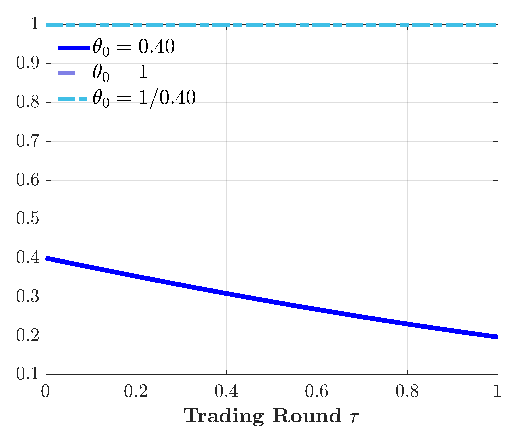
\includegraphics[width=0.8\linewidth]{NewCode/Figures/F_l_gammaplus_tau.eps}
\endminipage\minipage{0.33\textwidth}
\center{(b) Matching Rates $\psi^{-}$}\\[2pt]
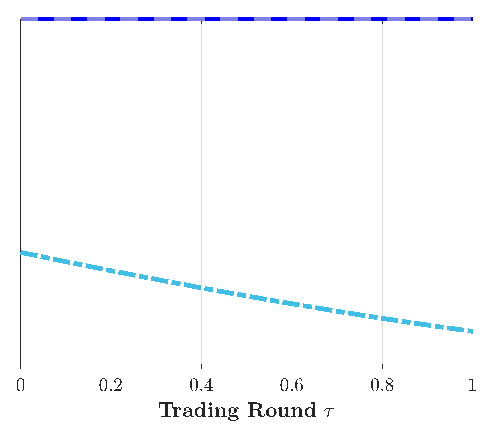
\includegraphics[width=0.78\linewidth]{NewCode/Figures/F_l_gammaminus_tau.eps}
\endminipage\minipage{0.33\textwidth}
\center{(c) Surplus $\Sigma_{\tau}$}\\[2pt]
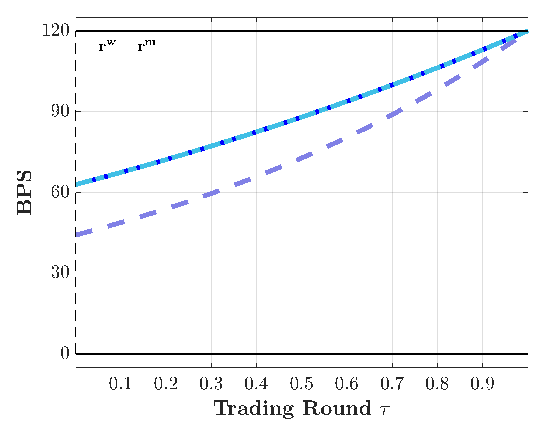
\includegraphics[width=0.8\linewidth]{NewCode/Figures/F_l_Surplus_tau.eps}
 \endminipage
\par\end{center}

\vspace{6pt}

\centering{}\minipage{0.33\textwidth}
\center{(d) Cost $\chi^{-}$} \\[2pt]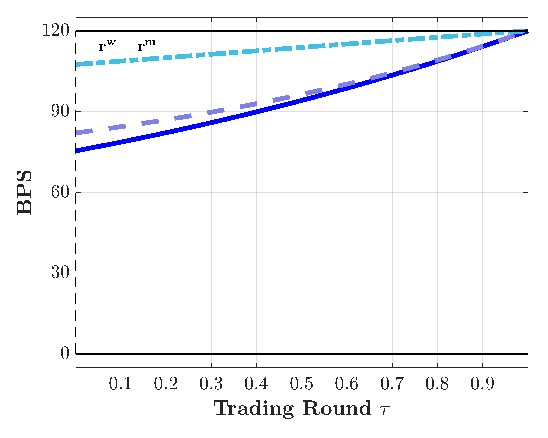
\includegraphics[width=0.8\linewidth]{NewCode/Figures/F_l_Chiminus_tau.eps}
\endminipage\minipage{0.33\textwidth}
\center{(e) Benefit $\chi^{+}$} \\[2pt]
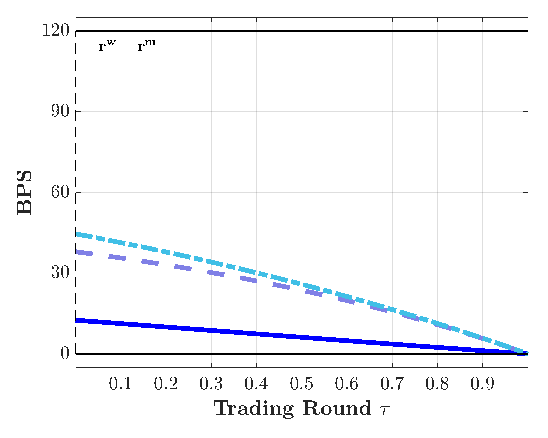
\includegraphics[width=0.8\linewidth]{NewCode/Figures/F_l_Chiplus_tau.eps}
\endminipage\minipage{0.33\textwidth}
\center{(f) Rate $r^{f}_{\tau}$} \\[2pt]
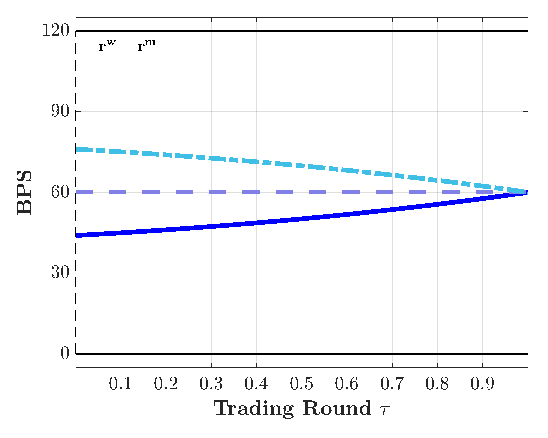
\includegraphics[width=0.8\linewidth]{NewCode/Figures/F_l_InterbankRate_tau.eps}\endminipage
\caption{\label{fig:F_InterbankDay-Leontief}\textbf{Leontief Example:} Trading at various rounds.}
\parbox[t]{1.\textwidth}{Note: $\theta_{0}=\theta$ is the initial market
tightness, the ratio of the initial aggregate deficit and
initial aggregate surplus. The example is calibrated with $\eta=0.5$,
$\bar{\lambda}=1.2$, $r^{w}-r^{m}=120$bps. See equation \eqref{eq:theta}.}
\end{figure}

\begin{figure}[H]
\begin{centering}
\minipage{0.33\textwidth}
\centering {(a) Matching Rate $\psi^{+}$} \\[2pt]
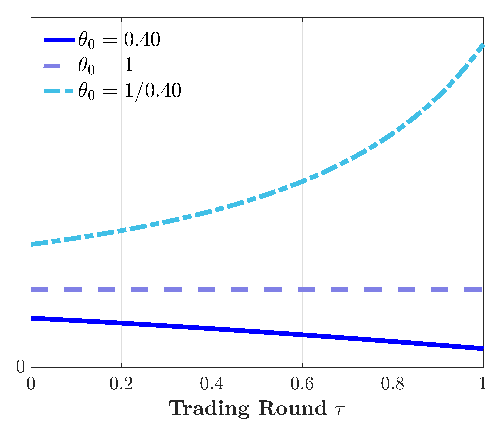
\includegraphics[width=0.8\linewidth]{NewCode/Figures/F_cd_gammaplus_tau.eps}
\endminipage\hfill
\minipage{0.33\textwidth}
\centering (b) Matching Rates $\psi^{-}$ \\[2pt]
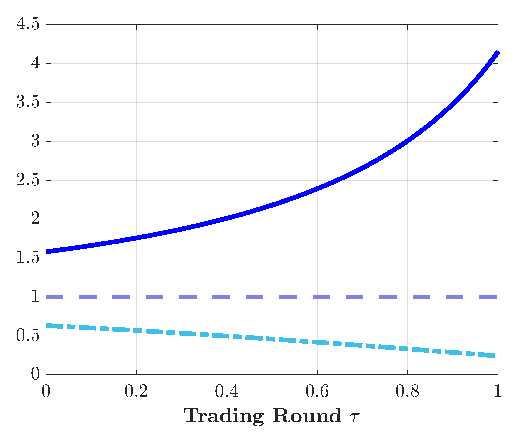
\includegraphics[width=0.8\linewidth]{NewCode/Figures/F_cd_gammaminus_tau.eps}
\endminipage\hfill
\minipage{0.33\textwidth}
\centering (c) Surplus $\Sigma_{\tau}$ \\[2pt]
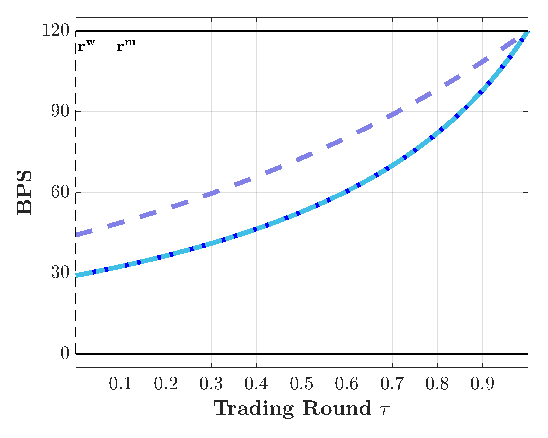
\includegraphics[width=0.8\linewidth]{NewCode/Figures/F_cd_Surplus_tau.eps}
\endminipage
\par\end{centering}

\vspace{10pt}

\begin{centering}
\minipage{0.33\textwidth}
\centering (d) Cost $\chi^{-}$ \\[2pt]
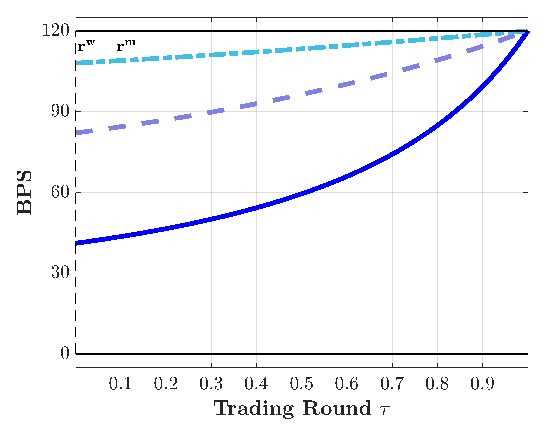
\includegraphics[width=0.8\linewidth]{NewCode/Figures/F_cd_Chiminus_tau.eps}
\endminipage\hfill
\minipage{0.33\textwidth}
\centering (e) Benefit $\chi^{+}$ \\[2pt]
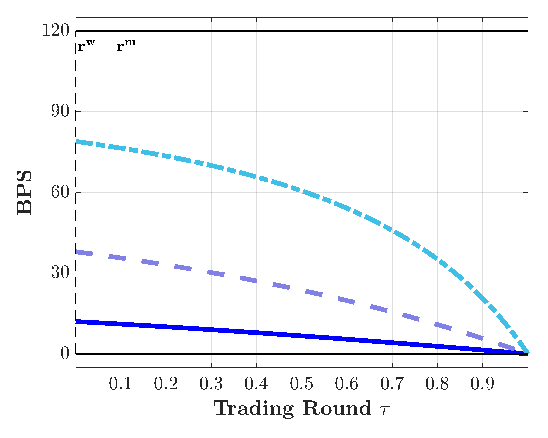
\includegraphics[width=0.8\linewidth]{NewCode/Figures/F_cd_Chiplus_tau.eps}
\endminipage\hfill
\minipage{0.33\textwidth}
\centering (f) OTC Rate $r^{f}_{\tau}$ \\[2pt]
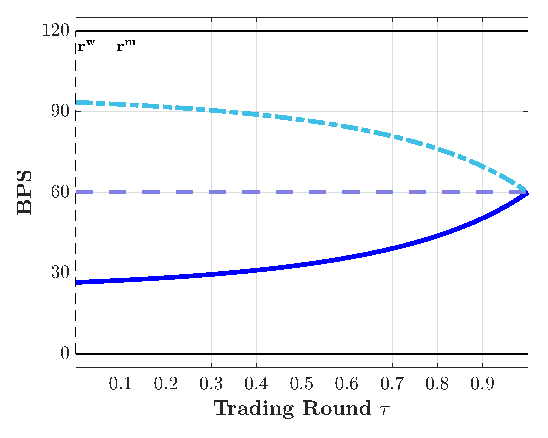
\includegraphics[width=0.8\linewidth]{NewCode/Figures/F_cd_InterbankRate_tau.eps}
\endminipage
\par\end{centering}
\vspace{5pt}
\caption{\label{fig:F_InterbankDay-CobbDouglas}Cobb-Douglas Example: Trading at various rounds}
\parbox[t]{1.\textwidth}{ \small{Note: $\theta_{0}=\theta$ is the initial
market tightness,  the initial aggregate deficit and the initial aggregate surplus. The example is calibrated with $\eta=0.5$,
$\bar{\lambda}=1.2$, $r^{w}-r^{m}=120$bps.}}

\end{figure}

\subsection{General Properties}

In this section, we present general properties of the OTC market and
liquidity-yield coefficients

\paragraph{Balanced Market Solution.}

Recall that when the OTC market is initially balanced, $\theta_{0}=1$, the market remains balanced throughout and, thus, matching rates are
equalized: $\psi_{\tau}^{+}=\psi_{\tau}^{-}=\left(1-\eta\right)\psi_{\tau}^{+}+\eta\psi_{\tau}^{-}=\bar{\lambda}$.
The following result follows from that observation:

\begin{corollary}[Balanced Market]\label{cor:balanced} For $\theta_{0}=1$,
 $\Sigma_{\tau}=\left(r^{w}-r^{m}\right)e^{-\bar{\lambda}\left(1-\tau\right)}$,
$r_{\tau}^{f}-r^{m}=\left(1-\eta\right)\left(r^{w}-r^{m}\right)$,
and $\left\{ \chi_{\tau}^{+},\chi_{\tau}^{-}\right\} =\left\{ \left(1-\eta\right)\left(\left(r^{w}-r^{m}\right)-\Sigma_{\tau}\right),\quad r^{w}-r^{m}-\eta\left(\left(r^{w}-r^{m}\right)-\Sigma_{\tau}\right)\right\} .$
\end{corollary}
When the market is balanced, the trading surplus is the terminal surplus, {$\left(r^{w}-r^{m}\right)$}, scaled by
the probability of no matches in the remaining time {$\left(1-\tau\right)$}.\footnote{This probability is an exponential with intensity $\bar{\lambda}$.}
The yield coefficients are affine in the surplus, with the average
cost of deficits increasing as time is running out---and the opposite for the surplus benefit. The yield coefficients balance exactly such that the average negotiated rates equal the one obtained under static
bargaining (i.e., a one-round bargaining problem).

\paragraph{Time Dilation.}

Another property of the OTC market equilibrium is time dilation: Let
$\theta\left(\tau,\theta_{0},\bar{\lambda}\right)$ denote the value
of market tightness $\theta$ at time $\tau$ given an initial condition
$\theta_{0}$ and efficiency $\bar{\lambda}$: the function representing
the solution \eqref{eq:ODE1}) as function of time, initial condition
and parameters; with the same notation for $\left\{ \gamma_{\tau}^{+},\gamma_{\tau}^{-},r_{\tau}^{f},\chi_{\tau}^{-},\chi_{\tau}^{+},\Sigma_{\tau}\right\} $.
Time dilation refers to the property that the passage of time is equivalent
to a reduction in efficiency:
\begin{proposition}[Time Dilation]\label{prop:time-dilation} Fix
$\tau,\tau'\in\left[0,1\right]$ such that $\tau'>\tau$. Then, 
\[
\theta\left(\tau',\theta_{0},\bar{\lambda}\right)=\theta\left(\frac{\tau'-\tau}{1-\tau},\theta\left(\tau,\theta_{0},\bar{\lambda}\right),\bar{\lambda}\left(1-\tau\right)\right).
\]
The same property holds for all the equilibrium objects $\left\{ \gamma^{+},\gamma^{-},\chi^{+},\chi^{-},r^{f}\right\} $.

\end{proposition}

Time dilation allows us to obtain the value of market tightness at an
instant $\tau'$, by computing first the value of market tightness
at a prior instant $\tau$: we can obtain the value at $\tau'$ by
(i) solving the equilibrium renormalizing time by the remaining time
$\left(1-\tau\right)$, (ii) scaling efficiency by the remaining time,
and (iii) setting the initial condition to $\theta_{\tau}$. This property is useful because it tells us that any property (e.g., monotonicity,
concavity, etc.) of the equilibrium functions at some moment in time
generalizes to all times. It also reveals the recursive nature of the market and shows that the normalization of time to the interval
$\left[0,1\right]$ is inconsequential. 

\paragraph{Symmetry.}

We established symmetry for the trading intensities from the symmetry
in the matching function. These property carries through to the market
rates and the yield coefficients: 
\begin{proposition}[Symmetry]\label{prop:symmetry} The OTC market
satisfies:
\begin{align}
\Sigma\left(\tau,\theta,\eta,\bar{\lambda}\right)&=\Sigma\left(\tau,\theta^{-1},1-\eta,\bar{\lambda}\right),\\ r^{f}\left(\tau,\theta,\eta,\bar{\lambda}\right)&=\left(r^{w}-r^{m}\right)-r^{f}\left(\tau\theta^{-1},1-\eta,\bar{\lambda}\right), \\
\chi^{-}\left(\tau,\theta,\eta,\bar{\lambda}\right)& =\left(r^{w}-r^{m}\right)-\chi^{+}\left(\tau,\theta^{-1},1-\eta,\bar{\lambda}\right)\\
\chi^{+}\left(\tau,\theta,\eta,\bar{\lambda}\right)&=\left(r^{w}-r^{m}\right)-\chi^{-}\left(\tau,\theta^{-1},1-\eta,\bar{\lambda}\right).
\end{align}

\end{proposition}
This symmetry states that if we can reverse the market tightness and
exchange the bargaining power of surplus and deficit sides, the
surplus function is the same. For the expected cost of being in deficit,
the benefit of a surplus, and the OTC rate, the same symmetry holds
relative to $r^{w}-r^{m}$. Panel (a) of Figure \ref{fig:symmetry}
plots the liquidity-yield coefficients for various values of $\eta$
and $\log\theta_{0}$ in the x axis. A rotation of 180 degrees around
the center of the figure gives the same figure once we swap $\eta$
for $\left(1-\eta\right)$. A similar pattern holds for the average
OTC rate. This property reveals that any asymmetry in outcomes
follows from asymmetries in assumed bargaining powers or the tightness.
This symmetry property implies that we can solve the model for $\theta<1$
and obtain solutions for $\theta>1$, immediately. Furthermore, as
we will see, many properties change exactly at $\theta=1$, due to
this property.

\begin{figure}[h]
\centering{}
\begin{minipage}[b]{.45\linewidth}
\center{(a) Symmetry Property} \\[4pt]
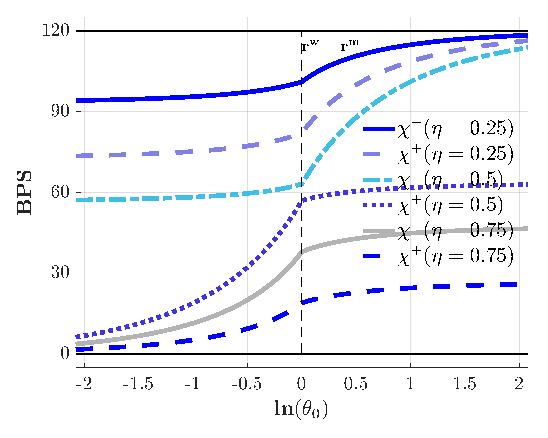
\includegraphics[width=1\linewidth]{NewCode/Figures/F_l_symmetry_theta.eps}
\end{minipage}
\hfill
    \begin{minipage}[b]{.45\linewidth}
    \center{(b) Walrasian Limit} \\[4pt]
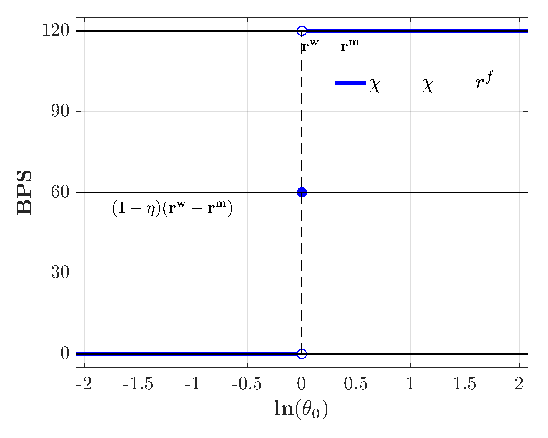
\includegraphics[width=1\linewidth]{NewCode/Figures/F_Walrasian_prices_theta.eps}
\end{minipage}
\caption{\label{fig:symmetry} Symmetry and Walrasian Limit Properties}

\parbox[b]{16cm}{\small{\emph{Note:} OTC rate and convenience yield coefficients as functions of $\theta_{0}$.
Trading at various rounds. Note: $\theta_{0}=\theta$ is the initial
market tightness defined as the ratio of the initial aggregate deficit
and initial aggregate surplus. The example in panel (a) is calibrated
using $\bar{\lambda}=0.8$, $r^{w}-r^{m}=120$bps. Panel (a) is calibrated
with $\eta=0.5$, $r^{w}-r^{m}=120$ bps. }} 
\end{figure}


\paragraph{Bargaining Power.}

Next, we characterize how the borrower's bargaining affects outcomes.

\begin{proposition}[Role of Bargaining Power]\label{prop:derivatives.eta}\label{prop:bargaininglimit}
The equilibrium objects $\left\{ \chi^{+},\chi^{-},\overline{r}^{f}\right\} $ are decreasing in $\eta$. In addition, at the extremes, we have that
\begin{itemize}
\item [i)] $\eta=1$: $\overline{r}^{f}=r^{m},\text{ }\left\{ \chi^{+},\chi^{-}\right\} =\left\{ 0,(1-\Psi^{-})(r^{w}-r^{m})\right\} ,$
\item [ii)] $\eta=0:$ $\overline{r}^{f}=r^{w},\text{ }\left\{ \chi^{+},\chi^{-}\right\} =\left\{ \Psi^{+}(r^{w}-r^{m}),(r^{w}-r^{m})\right\} .$
\end{itemize}
\end{proposition}

Thus, as $\eta$ increases, giving more bargaining power to borrowers,
rates at every round fall. Thus, liquidity yields are decreasing.
Regarding extrema, as borrowers extract all the matching surplus,
rates go to the reserve rate, and the average cost of deficits is the
penalty rate multiplied by the probability of matching in any round,
$\chi^{-}=(1-\Psi^{-})(r^{w}-r^{m})$; the opposite extreme follows
by symmetry.

\paragraph{Limiting cases: matching efficiency.}

We also derive the limiting properties as the market efficiency is
taken to its extreme values. 
\begin{proposition}[Efficiency Limits] \label{prop:LambdaLimit}
The OTC market equilibrium satisfies:
\begin{description}
\item [{Walrasian:}] As $\bar{\lambda}\rightarrow\infty$, the OTC market converges to its Walrasian market:
\end{description}
\begin{itemize}
\item [i)] If $\theta=1$, we have
\begin{align}
\Psi^{+}=\Psi^{-}=1, \quad \chi^{+} =   \left(r^{w} - r^{m} \right)\left(1 - \eta \right), \quad  \chi^{-}= \left(r^{w} - r^{m} \right)\left(1 - \eta \right). \quad \notag 
\end{align}

 \vspace{-13pt}
 
\item [ii)] If $\theta>1$, we have
\begin{align}
\Psi^{+}=1,\Psi^{-}=\theta^{-1}, \quad 
 \chi^{+}=\chi^{-}=\left(r^{w}-r^{m}\right),\quad\overline{r}^{f}=r^{w}. \notag 
 \end{align}
 
 \vspace{-13pt}
 
\item [iii)] If  $\theta<1$:
\begin{align}
{\Psi^{+}=\theta, \quad  \Psi^{-}=1 \quad 
  \chi^{+}=\chi^{-}=0,\quad\overline{r}^{f}=r^{m}.} \notag 
 \end{align}
\end{itemize}
\begin{description}
\item [{Static:}] As $\bar{\lambda}\rightarrow0$, the OTC market converges
to a static bargaining:{ $\Psi^{+}=\Psi^{-}=0$}
and 
\begin{align}
 \chi^{+}  =  0, \quad  ,\chi^{-} =\left(r^{w}-r^{m}\right)  , \quad \overline{r}^{f}=r^{m}+\left(r^{w}-r^{m}\right)(1-\eta). \notag 
 \end{align}
\end{description}
\end{proposition}

Proposition \ref{prop:LambdaLimit} shows that
as efficiency increases, the OTC market rate approaches a Walrasian
limit. In the Walrasian limit, if the market features an aggregate cash (scarcity
of funds) deficit, $\theta>1$, the average OTC market rate converges
to the borrowers' outside option, $r^{w}$. In the opposite case, as
$\theta<1$, the rate converges to $r^{m}$. Likewise, the liquidity
yields converge to the terminal trading surplus (in the case of an
aggregate cash deficit) and zero (otherwise). Panel (b) of Figure
\ref{fig:symmetry} plots the rates and liquidity yields at the Walrasian
limit.\footnote{In the knife-edge case where $\theta=1$, the average rate is an average
of outside options weighted by the bargaining power. In either case, the trading probability equals 1 for the shortest side of the market.} On the other hand, when matching efficiency approaches zero, rates and yields converge
to those of the static bargaining, and trade volume vanishes. 

\paragraph{Market Tightness. }


Another property of interest regards how the convenience yield function varies with market tightness.  We have the following corollary:
\begin{corollary}[Monotonicity in market tightness]\label{cor:monotonicity.theta}
In any OTC market equilibrium, $\left\{ \chi^{+},\chi^{-},\overline{r}^{f}\right\} $
are increasing in $\theta$.
\end{corollary}

The monotonicity of $\left\{ \chi^{+},\chi^{-},\overline{r}^{f}\right\} $
is intuitive. Market tightness captures the relative size of settlement
deficits. As deficits increase, lenders charge more for their funds
and can match with greater probability. Borrowers pay higher interest rates
on their OTC borrowings and are more likely to borrow from the last
resource. The change from concavity to convexity around $\theta=1$
follows immediately from the symmetry properties described above.

Next, we investigate the limit as market tightness approaches its
extrema. By symmetry, it is sufficient to discuss the limit $\theta_{0}\rightarrow0$.
Understanding this limit is important because it tells how the market
behaves as the \textit{aggregate} cash deficit vanishes. 
This limit highlights some subtle features of the model. One might initially expect that as one side of the market vanishes—say, as $\theta_0 \to 0$—the short side (i.e., borrowers) would capture the full surplus, leading rates and yield coefficients to approach zero. However, the actual limiting behavior is more nuanced, and this intuition holds only under specific conditions.

Whether the shortest side of the market extracts all surplus depends
on whether the intensive form of the matching function $\gamma\left(\cdot\right)$
is bounded above. Let $\bar{\gamma}\equiv\lim_{\theta\rightarrow0}\gamma\left(\theta^{-1}\right)$.
Clearly, $\bar{\gamma}$ is bounded for some matching functions, e.g.,
for the harmonic mean, $G\left(a,b\right)=\left(\frac{1}{2}a^{-1}+\frac{1}{2}b^{-1}\right)^{-b}$
but not for others, e.g., the Cobb-Douglas, $G\left(a,b\right)=a^{1/2}b^{1/2}$.
This bound is critical in determining the decay rate of $\theta$
as $\theta$ vanishes: 
\[
\frac{\dot{\theta}}{\theta}=-\bar{\lambda}\bar{\gamma}\quad\text{as}\quad\theta\rightarrow0.
\]

When the decay rate is finite, market tightness behaves as an exponentially
decaying function for $\theta$ close to zero. That is, the deficit
side of the market approaches zero, but is positive for all $\theta$
as $\theta\rightarrow0$. By contrast, if $\bar{\gamma}$ is unbounded,
the decay rate explodes, so the market tightness approaches zero extremely
fast as {$\theta\rightarrow0$}, leading
to a singularity point in the ODE where $\theta$ actually reaches
zero. Thus, $\theta_{\tau}$ in that case may approach zero in finite
time. This rate of decay, in turn, governs the behavior of the OTC
rates at the extrema. 

\begin{proposition}[Tightness Limits]\label{prop:LimitBehavior.Tightness}
The  convenience-yield function has the following limiting behavior:
\begin{enumerate}
  \renewcommand{\labelenumi}{\roman{enumi}.}
  
  \item $\theta \rightarrow 0$:  
  \begin{align*}
    \Psi^+ &= 0, & \Psi^- &= 1 - e^{-\bar{\lambda} \bar{\gamma}}, \\
    \chi^+ &= 0, & \chi^- &= (r^w - r^m) e^{-\bar{\lambda} \bar{\gamma} \eta}.
  \end{align*}
  
   \vspace{-12pt}
   
  \item $\theta \rightarrow \infty$:  
  \begin{align*}
    \Psi^+ &= 1 - e^{-\bar{\lambda} \bar{\gamma}}, & \Psi^- &= 0, \\
    \chi^+ &= (r^w - r^m)\left(1 - e^{-(1 - \eta)\bar{\lambda} \bar{\gamma}}\right), 
    & \chi^- &= r^w - r^m.
  \end{align*}

\end{enumerate}

\end{proposition}

As tightness approaches zero, the lenders' matching probability approaches
zero. Thus, $\chi^{+}\rightarrow0$. However, for the deficit side,
the short side of the market, whether the overall probability of matching
in the remaining rounds approaches one or remains less than one, depends
on the asymptotic decay rate, $\bar{\gamma}$. If this decay rate
is finite, although the deficit side is negligible relative to the
surplus side, the matching probability converges, $1-e^{-\bar{\lambda}\bar{\gamma}}$,
a number strictly less than one. As a result $\chi^{-}$ does not
vanish. If the asymptotic decay rate is unbounded, the matching probability
does converge to one and, in that case, $\chi^{-}$ will vanish. By
symmetry, the opposite occurs in the limit as $\theta\rightarrow\infty$.
These properties reflect on the OTC market rate.

Notice that if the asymptotic decay rate is infinite,
as market tightness vanishes, the average OTC rate approaches zero, which is
akin to giving all the bargaining power to the deficit side. 
Instead, if the asymptotic decay rate is finite, a trader with surplus
is able to extract some surplus in the improbable event that it
gets to match. This occurs because the deficit side has a positive
probability of not finding matches when $\bar{\gamma}$ is bounded.
By symmetry, the opposite occurs as the market tightness explodes. 


% Corollary (\ref{prop:LimitBehavior.Rates}) is relevant because it
% shows that even as all investors approach cash satiation, a situation
% where no investor is in deficit, OTC rates may exceed the rate on
% cash. This situation does not occur when the matching function assumed
% has an unbounded asymptotic decay rate. 
%

\subsection{CES (Generalized Means ) Matching Functions}

The properties above apply to all matching functions that satisfy Assumption \ref{ass:matching}. A special case is the constant-elasticity of substitution (CES) class (also
known as generalized means):\footnote{A Theorem by Kolmogorov states that the only functions that satisfy
symmetry and monotonicity satisfy that $G\left(a,b\right)=g^{-1}\left(\frac{1}{2}g\left(a\right)+\frac{1}{2}g\left(b\right)\right)$, for some monotone $g$.
A special case of such functions is the CES class.}
\[
G\left(a,b;p\right)=\left(\frac{1}{2}a^{p}+\frac{1}{2}b^{p}\right)^\frac{1}{p},
\]
where concavity requires $p\leq0$.\footnote{
The coefficient relates to the elasticity of substitution $\rho\geq0$
in production via $p=1/\left(1-\rho\right)$. For $p\leq0$, we have
$2^{1/p}G\left(a,b;p\right)\leq\min\left(a,b\right)$, so $\lambda_{N}<2^{1/p}$
guarantees weak exhaustion in the finite rounds case.} For $p=0$, the matching
function converges to a Cobb-Douglas (geometric mean), $G\left(a,b;p\right)=a^{1/2}b^{1/2}$,
while for $p=-\infty$, it converges to the Leontief matching function,
$\min\left\{ a,b\right\} $.\footnote{
Other common special cases are, $p=-1$, so that the matching function
becomes the harmonic mean: $G\left(a,b;p\right)=2\left(\frac{1}{a^{-1}+b^{-1}}\right).$
It is also known that for $q>p$, $G\left(a,b;p\right)<G\left(a,b;q\right)$.}

Figure~\ref{fig:F_comparison} compares CES matching functions. Panel (a) plots $\dot{\theta}/\theta$ as a function of $\theta$, showing that---except for the Cobb-Douglas case---the growth rate converges, indicating finite decay rates. Panel~(b) traces the time path $\theta_{\tau}$ from a common initial condition $\theta_0$. Only under Cobb-Douglas does $\theta_{\tau}$ reach zero; in all other cases, tightness decays toward zero but never vanishes in finite time.\footnote{Indeed, the solution to $\theta_{\tau}$ may reach zero in some finite time $\tau<1$ if and only if $p=0$ (the matching function is Cobb-Douglas).}
The plots illustrate Proposition~\ref{prop:theta.ode.props}: tightness decays faster for higher values of $p$.

Panels~(c) and~(d) show liquidity yields as a function of $\log(\theta_0)$. Only for the Cobb-Douglas case the yield coefficients vanish (i.e., $r^w - r^m = 0$) for sufficiently small $\theta_0$. This underscores that Cobb-Douglas is a knife-edge case within the CES family ($p \leq 0$), uniquely featuring infinite decay. Hence, it is the only specification where OTC rates and liquidity premia can be fully extinguished in finite time. In that sense, it delivers full cash-satiation: all surpluses are reallocated across trading rounds, unlike a situation where there is no trade simply because no investors have a deficit.
\begin{figure}[h!]
    \begin{minipage}[b]{.45\linewidth} 
        \center{(a)  Growth rate of $\theta_{\tau}$} \\[4pt]
        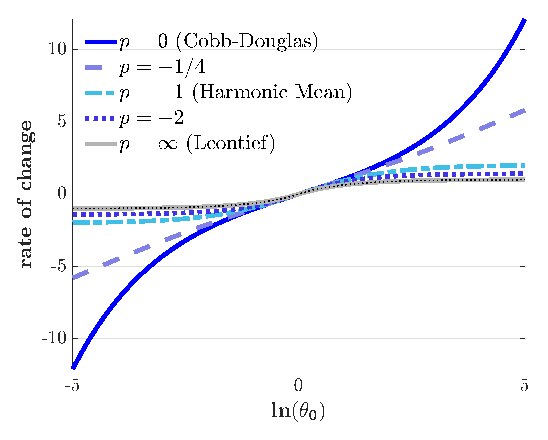
\includegraphics[width=1\linewidth]{NewCode/Figures/F_growthrate.eps}
    \end{minipage}
    \hfill
    \begin{minipage}[b]{.45\linewidth}
    \center{(b) Evolution of $\theta_{\tau}$} \\[4pt]
    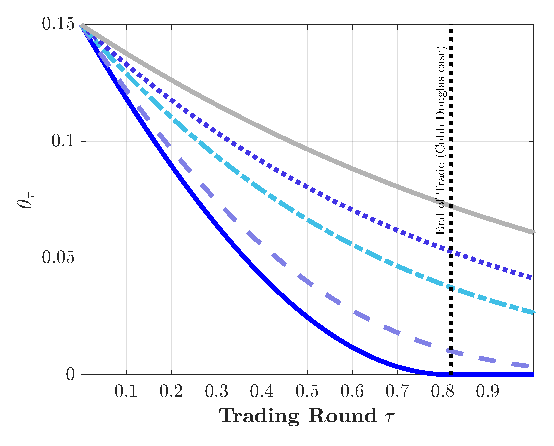
\includegraphics[width=1\linewidth]{NewCode/Figures/F_trajectories.eps}
    \end{minipage}
    
\vspace{10pt}

\begin{minipage}[b]{.45\linewidth}

\center{(c) $\chi^{+}$} \\[4pt]

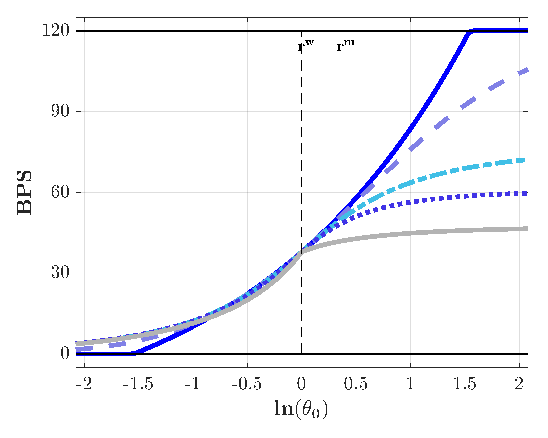
\includegraphics[width=1\linewidth]{NewCode/Figures/F_chip_comp.eps}
\end{minipage}
\hfill
\begin{minipage}[b]
{.45\linewidth}

\center{(d) $\chi^{-}$}  \\[4pt]

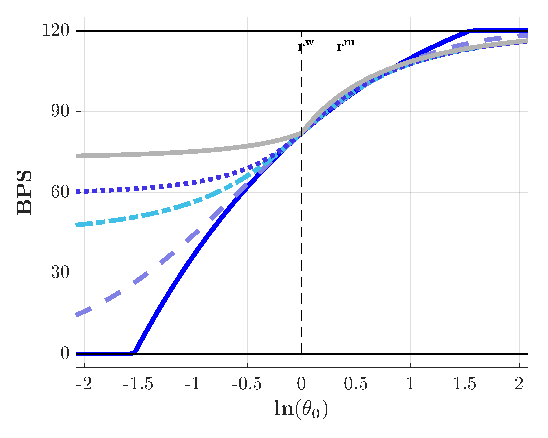
\includegraphics[width=1\linewidth]{NewCode/Figures/F_chim_comp.eps}
\end{minipage}
\caption{\label{fig:F_comparison}Comparison Across CES matching functions.
}

\parbox[b]{16cm}{\small \emph{Note:} $\theta=\theta_{0}$ is the initial market tightness. The example
is calibrated with $\eta=0.5$, $\bar{\lambda}=1.2$, $r^{w}-r^{m}=120$bps
in all cases.}
\end{figure}

\subsubsection*{Analytical Cases: Cobb-Douglas and Leontief }

\label{sec:closed-form}

We now present fully analytical solutions to the OTC market for the Cobb-Douglas and Leontief cases. Table \ref{tab:closedforms} presents the solution for the market tightness
in the Cobb-Douglas and Leontief cases, respectively.

\begin{table}[hb]
\caption{\label{tab:closedforms} Analytical Formulas:} 
\centering 
\global\long\def\arraystretch{1.4}%
\begin{tabular}{|c|c|c|}
\hline 
\textbf{Matching} & Cobb-Douglas ($p=0$) & Leontief ($p=-\infty$)\tabularnewline
\hline 
\boldmath$\theta(\tau), \  \tau\in\left[0,T\right]$

& $\left(\dfrac{\left(1+\sqrt{\theta_{0}}\right)e^{-\bar{\lambda}t}-\left(1-\sqrt{\theta_{0}}\right)}{\left(1+\sqrt{\theta_{0}}\right)e^{-\bar{\lambda}t}+\left(1-\sqrt{\theta_{0}}\right)}\right)^{2}$ & $\left\{ \begin{array}{cc}
1+\left(\theta-1\right)e^{\bar{\lambda}\tau}, & \theta>1\\
\\\dfrac{\theta_{0}}{\theta_{0}+(1-\theta_{0})e^{\bar{\lambda}\tau}}, & \theta<1
\end{array}\right.$\tabularnewline
\hline 
\boldmath{$T$} & $\min\left\{ \dfrac{1}{\bar{\lambda}}\log\left(\left|\dfrac{1+\sqrt{\theta_{0}}}{1-\sqrt{\theta_{0}}}\right|\right),\,1\right\} $ & $\infty$\tabularnewline
\hline 
\boldmath$\Psi^{+}$ & $1-e^{-\bar{\lambda}T}\left(\dfrac{\left(1+\sqrt{\theta_{0}}\right)+\left(1-\sqrt{\theta_{0}}\right)e^{\bar{\lambda}T}}{\left(1+\sqrt{\theta_{0}}\right)+\left(1-\sqrt{\theta_{0}}\right)}\right)^{2}$ & $\begin{cases}
1-e^{-\bar{\lambda}}, & \theta_{0}\geq1\\
\\\theta_{0}(1-e^{-\bar{\lambda}}), & \theta_{0}<1
\end{cases}$\tabularnewline
\hline 
\boldmath$\Psi^{-}$ & $1-e^{-\bar{\lambda}T}\left(\dfrac{\left(1+\sqrt{\theta_{0}}\right)-\left(1-\sqrt{\theta_{0}}\right)e^{\bar{\lambda}T}}{\left(1+\sqrt{\theta_{0}}\right)-\left(1-\sqrt{\theta_{0}}\right)}\right)^{2}$ & $\begin{cases}
(1-e^{-\bar{\lambda}})\theta_{0}^{-1}, & \theta_{0}>1\\
\\1-e^{-\bar{\lambda}}, & \theta_{0}\leq1
\end{cases}$\tabularnewline
\hline 
\end{tabular}

\vspace{0pt}
\begin{center}
\parbox[t]{0.99\textwidth}{ \small{\emph{Note:} Closed-form
solutions for $\theta(t)$, stopping time $T$, and matching probabilities
$\Psi^{+}$,$\Psi^{-}$.}}
\end{center}
\end{table}
The Cobb-Douglas and Leontief cases display qualitatively distinct trading dynamics. Under Leontief matching, the short side's trading probabilities are exponentially distributed, independently of the initial tightness. Thus, $\theta_{\tau}$ never vanishes fully throughout the trading session. Instead, $\theta_{\tau}$ follows a logistic path. In the Cobb-Douglas case, the short side of the market may vanish before the trading time is over, if the stop time $T$ in the
Table \ref{tab:closedforms} is $T<1$; evaluating the formula for $\theta_{\tau}$ at the stopping
time, $\tau=T$, yields zero or infinity, which is consistent with
the end of trade.\footnote{The formula for $\theta_{\tau}$ is actually associated with the hyperbolic
tangent function.} Hence, in the Cobb-Douglas case, trade stops if
the initial tightness is sufficiently unbalanced:
\[
\theta_{0}\not\in\left[\left(\frac{\exp\left(\bar{\lambda}\right)-1}{\exp\left(\bar{\lambda}\right)+1}\right)^{2},\left(\frac{\exp\left(\bar{\lambda}\right)+1}{\exp\left(\bar{\lambda}\right)-1}\right)^{2}\right].
\]
Equivalently, trade vanishes in finite time if efficiency is sufficiently high: $\bar{\lambda}>\log\left(\left|\dfrac{1+\sqrt{\theta_{0}}}{1-\sqrt{\theta_{0}}}\right|\right)$. 

While the solution for the path of market tightness is different in the Leontief
and Cobb-Douglas cases, the yield coefficients turn out to have the same expressions
as a function of the initial tightness, $\theta$, and the terminal tightness, $\bar{\theta}$, eventhough the terminal values are very different:

\begin{proposition}
    
\label{prop:analytic.solution-2} Fix, $\theta=\theta_{0}$
and compute $\bar{\ensuremath{\theta}}=\theta_{1}$ under the Cobb-Douglas
and Leontief cases. In either case, the convenience yield coefficients are:{
\[
\begin{array}{ll}
\chi^{+} = \left(r^{w}-r^{m}\right)\left(\dfrac{\bar{\theta}-\bar{\theta}^{\eta}\theta^{1-\eta}}{\bar{\theta}-1}\right), &
\chi^{-} = \left(r^{w}-r^{m}\right)\left(\dfrac{\bar{\theta}-\bar{\theta}^{\eta}\theta^{-\eta}}{\bar{\theta}-1}\right)
\end{array}
\]
}
\end{proposition}
The solution to $\left\{ \chi^{+},\chi^{-}\right\} $
is a continuous function of the initial tightness and the terminal
tightness, $\theta$ and $\bar{\theta}$. $\left\{ \chi^{+},\chi^{-}\right\} $
are always positive and bounded by the terminal surplus, $r^{w}-r^{m}$,
as expected. We furthermore obtain the OTC rate as
a weighted average of the cash rate and discount rate:
\begin{equation}
\overline{r}^{f}=\phi\left(\theta\right)r^{m}+(1-\phi\left(\theta\right)\mathbf{)}r^{w},\text{ where }\phi\left(\theta\right)=\frac{\left(\bar{\theta}/\theta\right)^{\eta}-\theta}{\bar{\theta}/\theta-1}\phi\left(\theta\right)\in\left[0,1\right].\label{eq:OTC.rate}
\end{equation}
As in \cite{AL15-ECMA}, the term $\phi\left(\theta\right)$ acts as an endogenous bargaining
rate: unlike static bargaining, this bargaining rate depends on the
evolution of outside options. {$\phi\left(\theta\right)$}
compactly captures the information from the matching function and
the bargaining process. We further verify that $\lim_{\theta\rightarrow1}\phi\left(\theta\right)=\eta$,
consistent with the balanced-market outcome above. 

The behavior of the yield coefficients and the average rate as a function
of $\log\left(\theta_{0}\right)$ is depicted in Figure \ref{fig:closed.formfigures}.
Panels (a) and (b) depict the outcomes as functions of the initial
condition for the Leontief and Cobb-Douglas cases. Both figures have
sigmoid-like patterns, but the differences regarding concavity, and
the limits as $\theta$ moves to its extreme are clear. In the Cobb-Douglas case, as market tightness becomes sufficiently unbalanced, the short side of the market trades is fully matched and, hence, trade is efficient. In such cases, the OTC rates are constant and coincide with their Walrasian limit.

\begin{figure}[H]

    \begin{minipage}[b]{.49\linewidth} 
    \center{(a) Leontief}
    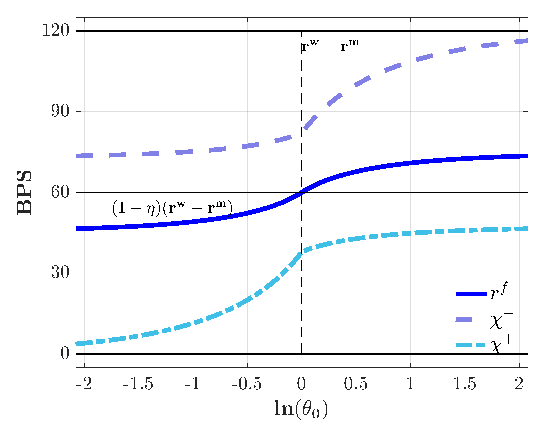
\includegraphics[width=1\linewidth]{NewCode/Figures/F_l_prices_theta.eps}
\end{minipage}\hfill{}    \begin{minipage}[b]{.49\linewidth}
\center{(b) Cobb-Douglas}
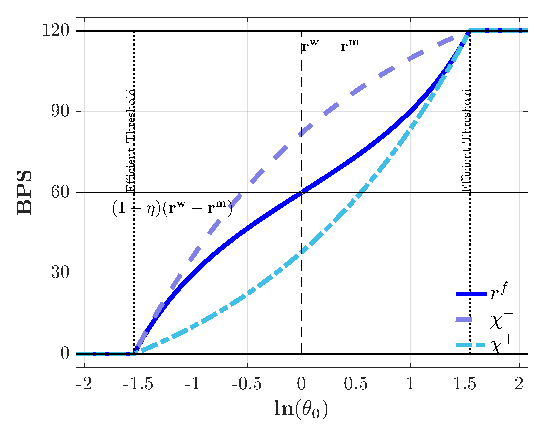
\includegraphics[width=1\linewidth]{NewCode/Figures/F_cd_prices_theta.eps}
\end{minipage}
\centering{}\caption{\label{fig:closed.formfigures}  Analytic Solutions:  OTC rates
and yield coefficients for Leontief and Cobb-Douglas Matching Functions.}
\parbox[t]{\textwidth}{\footnotesize
\textit{Note:} The OTC rate and convenience yield coefficients are plotted as
functions of $\theta_{0}$. $\theta_{0}=\theta$ is the initial market tightness, defined as the ratio of the initial aggregate deficit and
initial aggregate surplus. Both panels are calibrated using $\eta=0.5$, $\bar{\lambda}=1.2$,
$r^{w}-r^{m}=120$bps. }
\end{figure}

\FloatBarrier

 \section{ Applications}

\label{sec:applications}


\subsection{Portfolio choices and convenience yields}

We now study optimal portfolios in the presence of settlement risk. We
maintain the assumption that all returns are exogenous, except for
the endogenous OTC rate $\bar{R}^{f}$ . Investor preferences are represented
by
\begin{equation}
\mathbb{E}_{0}\sum_{t=0}^{\infty}\beta^{t}u(c_{t}),
\end{equation}
where $\beta<1$ is the time discount factor, and $u\left(c\right)=\frac{c^{1-\gamma}-1}{1-\gamma}$
is the utility function over the consumption good with $\gamma\ge0$.
As described in Section \ref{sec:model}, each period, investors start with an initial
wealth $e$, which depends on previous portfolio choices and the realization
of returns, and choose their portfolio decisions subject to the budget
constraint \eqref{eq:e.accumulation} We present below the problem
of the investor in recursive form. We use $\AggS$ to denote an aggregate
state.

\begin{problem}[Investor's Problem]The savings-portfolio problem
is:
\begin{equation}
V_{t}(e,\AggS)=\max_{\left\{ c,\left\{ \tilde{a}_{t+1}^{i}\right\} _{i\in\mathbb{I}},\tilde{m_{t+1}}\right\} }u(c)+\beta\mathbb{E}\left[V_{t+1}(e_{t+1},\AggS')\right],\label{eq:bellman-single}
\end{equation}
subject to: \eqref{eq:e.accumulation}, \eqref{eq:surplus}, and \eqref{eq:total.E.returns}.

\end{problem}

In the investor's problem, $\mathbb{E}$ denotes the expectation operator
with respect to the idiosyncratic liquidity shock in the settlement
stage in the current period and the next period's realization of returns.
Because preferences are homothetic and constraints linear, the problem admits portfolio separation: consumption (or dividends) can be chosen independently of portfolio weights, which themselves depend only on returns and settlement risks, not on total equity.\footnote{See Proposition 3 of \citet{BB17} for a full characterization.}

The investor chooses portfolio weights on assets $\left\{ a^{i}\right\} $ and the cash asset $m$ to maximize the expected utility of returns, incorporating both standard asset returns and convenience yields arising from settlement frictions.\footnote{
The weights are defined as portfolio holdings relative to equity.
With abuse of notation, we denote the weights with the same notation
as the holdings.
}
\begin{equation}
\max_{\substack{m,\left\{ a^{i}\right\} _{i\in\mathbb{I}}}
}\left(\mathbb{E}\left[\sum_{i\in\mathbb{I}}R_{t+1}^{i}\left(\AggS'\right)a^{i}+R_{t+1}^{m}(\AggS')m+\chi_{t+1}\left(s\left(\left\{ a^{i}\right\} _{i\in\mathbb{I}},m,\left\{ \omega_{t+1}^{i}\right\} _{i\in\mathbb{I}}\right);\theta_{t}\right)\right]^{1-\gamma}\right)^{\frac{1}{1-\gamma}}\label{eq:portf-1}
\end{equation}
subject to:
\[
\sum_{i\in\mathbb{I}}a^{i}+m=1
\]
where we make explicit the dependence of the convenience yield on the market
tightness, with a slight abuse of notation.

Figure \ref{fig:liquidity_yields} illustrates the forces underlying the portfolio problem.
Panel (a) of Figure \ref{fig:liquidity_yields}
shows how portfolio choice affects settlement risk through the
convenience yield function $\chi\left(s;\theta\right)$. The purple kinked
function represents $\chi\left(s;\theta\right)$, which maps settlement
positions $s$ into additional payoffs. When $s<0$ (settlement deficit),
investors face average borrowing costs $\chi^{-}$; when $s>0$ (surplus),
they earn lending returns with slope $\chi^{+}$. The asymmetry in
the yield coefficients reflects higher penalty rates for emergency
borrowing than returns on surplus lending. The panel shows two settlement
distributions arising from different portfolio choices. The high-risk
portfolio (red, dashed) generates a wide distribution of settlement
needs, with significant probability mass in deficit regions. The low-risk
portfolio (blue, solid) concentrates settlement positions at higher
values. Due to the kink at zero, the high-settlement risk portfolio
incurs expected losses even when distributions have zero mean. This
illustrates a key insight: assets that generate volatile settlement
needs command convenience yields to compensate for these expected
losses, even for risk-neutral investors. Panel (b) of Figure \ref{fig:liquidity_yields}
illustrates shows how individual portfolio choices affects the liquidity
yield function$\chi\left(s;\theta\right)$ of others. 

\begin{figure}[h]
\centering
%\begin{minipage}{0.48\textwidth}
\centering
\begin{tikzpicture}[thick,scale=0.7, every node/.style={transform shape}]
% First figure (original)
% Axes
\draw[->, black] (-2,0) -- ( 8, 0) node[above]{Settlement position $(s)$};
\draw[->, black] (3.35,-3.5) -- (3.35, 6.5) node[left]{$\chi(s)$};
% Zero point
\node[black, below right] at (3.35,0){$0$};
% Region labels (below x-axis)
\node[align=center,black] at (6.5,-0.8){Surplus\\Region};
\node[align=center,black] at (0.5,-0.8){Deficit\\Region};
\node[align=center,black] at (4.5,6.2){Settlement\\Distribution};
\draw[<-, very thick, purple] (-1.5,-4.5) -- (3.35, 0); % Steep negative slope for deficit
\draw[->, very thick, purple] (3.35,0) -- (7,1.5); % Gentle positive slope for surplus
% Distribution curves (no shading)
\draw[red, dashed] (-1.5,0) to [out=0,in=-90] (2.5,4.5);
\draw[red, dashed] (2.5,4.5) to [out=90,in=180] (3.0,5.5);
\draw[red, dashed] (3.0,5.5) to [out=0,in=90] (3.5,4.5);
\draw[red, dashed] (3.5,4.5) to [out=-90,in=180] (6.0,0);
\draw[blue,thick] (0.5,0) to [out=0,in=-90] (3.5,4.5);
\draw[blue, thick] (3.5,4.5) to [out=90,in=180] (4.0,5.5);
\draw[blue, thick] (4.0,5.5) to [out=0,in=90] (4.5,4.5);
\draw[blue, thick] (4.5,4.5) to [out=-90,in=180] (7.0,0);
% Labels for distributions (moved away from y-axis)
\draw[red,thick,->] (2.6,5.3) -- (1.5,5.3) node[left]{High settlement risk};
\draw[blue,thick,->] (4.4,5.3) -- (5.5,5.3) node[right]{Low settlement risk};
% Slopes labels
\node[purple] at (-0.5,-2.9) {$\chi^-$};
\node[purple] at (5.7,1.5) {$\chi^+$}; % Moved closer to the curve
% Vertical line at zero
\draw[black, dotted] (3.35,-3.5) -- (3.35,6.5);
\end{tikzpicture}
%\center{(a) Portfolio choice and liquidity yields}
% \end{minipage}
% \hfill
% \begin{minipage}{0.48\textwidth}
% \centering
% \begin{tikzpicture}[thick,scale=0.5, every node/.style={transform shape}]
% % Second figure (with rotation)
% % Axes
% \draw[->, black] (-2,0) -- ( 8, 0) node[above]{Settlement position $(s)$};
% \draw[->, black] (3.35,-3.5) -- (3.35, 6.5) node[left]{$\chi(s)$};
% % Zero point
% \node[black, below right] at (3.35,0){$0$};
% % Region labels (below x-axis)
% \node[align=center,black] at (6.5,-0.8){Surplus\\Region};
% \node[align=center,black] at (0.5,-0.8){Deficit\\Region};
% % Original convenience yieldfunction
% \draw[<-, thick, purple] (-1.5,-4.5) -- (3.35, 0);
% \draw[->, thick, purple] (3.35,0) -- (7,1.5);
% % Rotated convenience yieldfunction (tighter market)
% \draw[<-, very thick, orange, dashed] (-1.5,-5.5) -- (3.35, 0);
% \draw[->, very thick, orange, dashed] (3.35,0) -- (7,2.1);
% % Slopes labels for original function
% \node[purple] at (-0.5,-2.9) {$\chi^-$};
% \node[purple] at (5.7,1.5) {$\chi^+$};
% % Slopes labels for rotated function
% \node[orange] at (-1.8,-3.5) {$\tilde{\chi}^-$};
% \node[orange] at (6.5,2.1) {$\tilde{\chi}^+$};
% % Legend
% \node[purple] at (2,4.5) {Baseline};
% \node[orange] at (2,3.8) {Tighter market};
% % Vertical line at zero
% \draw[black, dotted] (3.35,-3.5) -- (3.35,6.5);
% \end{tikzpicture}
% \center{(b) Market tightness and liquidity yields}
% \end{minipage}
\caption{Convenience yield function $\chi(s)$ and settlement risk.  }
%Panel (b) illustrates how market tightness (driven by others' portfolio choices) rotates the convenience yieldfunction, increasing both borrowing costs and lending returns.}
\label{fig:liquidity_yields}
\end{figure}

\paragraph*{Convenience yields.}

Let us define $\chi_{s}\equiv\frac{\partial\chi}{\partial s}$ which
is equal to $\chi^{+}$ if $s\ge0$ and $\chi^{-}$otherwise. Taking
first-order conditions in the portfolio problem \eqref{eq:portf-1}, and assuming strictly interior portfolio positions, we obtain
\begin{align}
\underset{\text{premium}}{\underbrace{\mathbb{E}_{X}\left[R^{i}\right]-R^{m}}}
& \ = \ 
\underset{\text{first-order liquidity premium}}{
\underbrace{
\mathbb{E}_{X,\omega}\left[\chi_{s}\frac{\partial s}{\partial m}
-\chi_{s}\frac{\partial s}{\partial a^{i}}\right]
}
}
-
\underset{\text{liquidity risk premium}}{
\underbrace{
\frac{
\mathbb{COV}_{X,\omega}\left[
\left(R^{e}\right)^{-\gamma},
\chi_{s}\frac{\partial s}{\partial m}
-\chi_{s}\frac{\partial s}{\partial a^{i}}
\right]
}{
\mathbb{E}_{X,\omega}\left[\left(R^{e}\right)^{-\gamma}\right]
}
}
} \notag \\
&\quad 
-
\underset{\text{conventional risk premium}}{
\underbrace{
\frac{
\mathbb{COV}_{X,\omega}\left[
\left(R^{e}\right)^{-\gamma},
R^{i}\left(X\right)
\right]
}{
\mathbb{E}_{X,\omega}\left[\left(R^{e}\right)^{-\gamma}\right]
}
}
} 
\label{eq:liquidity.premiumcov} 
\end{align}

The optimal portfolio equalizes the marginal utility-weighted returns across assets, accounting for both price risk and liquidity risk due to settlement.
The left-hand side is the difference in the expected return of asset
$i$ relative to cash. At an optimal solution, the representation
in \eqref{eq:liquidity.premiumcov} shows that this asset's premium
equals the sum of a convenience yield (liquidity premium) and a conventional
risk premium. Thus, the equation captures a trade-off between expected
return differentials against settlement risk and a conventional risk
premium. The former emerges because asset $a^{i}$ exposes the investor
to settlement risk, whereas a larger $m$ provides liquidity. In particular,
in the case of a negative settlement shock, the investor obtains a
higher return on cash compared to a less liquid asset and vice-versa.
Assets that induce greater liquidity risk command a greater premium.

The liquidity premium term can be further unpacked into two terms:
The first term captures how changes in the portfolio affect the expected
settlement costs.\footnote{Note that $\chi$ is differentiable almost everywhere. While changing the portfolio affects, at the margin, the probability
of being short or long, this does not enter into the optimality condition
because the bank obtains the same marginal payoff (i.e., zero) evaluated
at the threshold $\omega^{\ast}$. Using Leibniz's, we can show that
the effect disappears given that $s=0$ when the shock is $\omega^{\ast}$.} This term is present under risk neutrality. The terms are negative
even when the cash position is zero in expectation because the liquidity
yield function is concave. In turn, the second term captures
the covariance term between liquidity payoffs and the discount factor: when the investor is risk-averse, states with negative returns penalize
additional settlement costs.

There are some important lessons here: First, settlement risks induce
determinate portfolios even among risk-neutral investors. Unlike standard
portfolio problems where the riskiness of assets is given, here, by
choosing its cash position, investors control the amount of risk.
Given the concavity of $\chi$, investors must be compensated with
returns in order to hold portfolios that are more exposed to settlement
risk. Second, the standard risk-adjustment 
insufficient to price the risk associated with an asset. Crucially,
without considering the cash needs induced by an
asset, the return in payoffs is not enough to capture the full extent
of risk. Conversely, convenience yields cannot be treated as pricing
factors independent of risk, because the correlation between the riskiness
of the asset and the liquidity needs must be considered. Another possible
application of the theory is to investigate how the equity premium
puzzle \citep{MERH/PRES/85} is impacted by the presence of convenience
yields.

\subsection{Parameter Identification}

An important empirical question is how to identify the underlying OTC market parameters
and settlement risk from observable data? Our analytical formulas
reveal that the average OTC rate $\bar{r}^{f}$ and the liquidity
yield coefficients $\left\{ \chi^{+},\chi^{-}\right\} $ depend on
three key elements: market tightness $\theta$ (which, given portfolios,
reflects the distribution of unobservable settlement shocks), matching
efficiency $\bar{\lambda}$, and bargaining power $\eta$. However, these parameters are not directly observable. This section develops
an approach to infer them from two potential sources of data: (i)
convenience yields on liquid assets, which reveal the shadow value
of liquidity, and (ii) OTC market outcomes, particularly rate dispersion
and trading volumes.

An estimation of these structural parameters is important because it helps quantify the sources of variation in convenience yields over time and across assets. Furthermore, this estimation enables counterfactual analyses. In what follows, we focus for the most part on the Leontief matching function, which yields particularly sharp comparative statics that facilitate identification. 

\paragraph{Market tightness.}

It is worth recalling a key result from our earlier analysis. As established
in Corollary \ref{cor:monotonicity.theta}, the convenience yield coefficients
and the average OTC rate $\left\{ \chi^{+},\chi^{-},\overline{r}^{f}\right\} $
are all monotonically increasing in market tightness $\theta$. This
monotonicity enables identification of $\theta$ from observable data.
For instance, the convenience yield on illiquid bonds \eqref{eq:illiquidbond.premium})
depends on a weighted sum of the liquidity coefficients, which is
also monotonic in $\theta$ given portfolios. Similarly, the average
OTC rate increases monotonically with $\theta$. Once we identify
$\theta$ from these observables, we can back out parameters of the
unobserved settlement shock distribution, such as the variance of
withdrawal risk or the frequency of margin calls. Note that the net
interest margin in equation \eqref{eq:deposit.premium}) depends on
a weighted difference of the yield coefficients, which need not be
monotonic in $\theta$.\footnote{The curvature properties of the yield coefficients---whether convex
or concave---may provide additional information.}

\paragraph{Matching efficiency.}
Let us now turn to the comparative static with respect to the efficiency parameter $\bar{\lambda}$.

\begin{proposition}[Comparative Statics in Leontief Case]\label{prop:derivatives.lambda}
If the matching function is Leontief, we have that:
i) Let $\theta<1$, then $\chi^{-}$ is decreasing in $\bar{\lambda}$,
$\overline{r}^{f}$ is decreasing in $\bar{\lambda}$, and $\chi^{+}$
is non-montonic in $\bar{\lambda}$.
ii) Let $\theta>1$, then $\chi^{+}$ is increasing in $\bar{\lambda}$,
$\overline{r}^{f}$ is increasing in $\bar{\lambda}$, and $\chi^{-}$
is non-montonic in $\bar{\lambda}$.
iii) Let $\theta=1$, then
\[
\frac{\partial\chi^{+}}{\partial\bar{\lambda}}=(r^{w}-r^{m})\left(1-\eta\right)\frac{\partial\Psi^{+}}{\partial\bar{\lambda}}>0,\qquad\frac{\partial\chi^{-}}{\partial\bar{\lambda}}=-(r^{w}-r^{m})\eta\frac{\partial\Psi^{-}}{\partial\bar{\lambda}}<0.
\]

\end{proposition}

The comparative static reveals a subtle but important insight: convenience yields may be non-monotonic in the matching efficiency.
When markets are tight
($\theta>1$), improving matching efficiency has two opposing effects: it increases the probability that deficit investors find lenders (reducing
their borrowing costs), but it also strengthens lenders' bargaining
position, raising equilibrium rates. The net effect on $\chi^{-}$
depends on which force dominates. This non-monotonicity means that
higher convenience yields need not signal market dysfunction---they
could reflect improved matching that benefits the scarce side of the
market. The same non-monotonic pattern
characterizes the average OTC rate $\overline{r}^{f}$. Figure \ref{fig:efficiency.compstat}
illustrates these relationships: Panel (a) confirms our theoretical
results for the Leontief case, while Panel (b) demonstrates that this
pattern extends to the Cobb-Douglas matching function, suggesting it is a robust feature of OTC markets outside of the Leontief case. 

The non-monotonicity of rates and liquidity premia with respect to efficiency implies that convenience yields cannot be interpreted mechanically as evidence of worsening market efficiency. To see this, consider the first-order liquidity premium in equation \eqref{eq:liquidity.premiumcov} for an asset that does not expose investors to settlement risk, i.e., $\frac{\partial s}{\partial a^{i}}=0$. In that case, the premium reduces to $\mathbb{E}{X,\omega}\left[\chi{s} \right]$. An increase in this premium could be consistent with two opposite interpretations. On the one hand, it might signal weaker OTC efficiency, raising investors’ demand for cash as insurance against settlement needs. On the other hand, it could reflect greater efficiency, which enhances the option value of holding cash to exploit lending opportunities. Thus, higher observed convenience yields do not unambiguously point to deteriorating trading efficiency.
\begin{figure}[tbh!]
   \begin{minipage}[b]{.45\linewidth} 
   \center{(a) Leontief } \\[4pt] 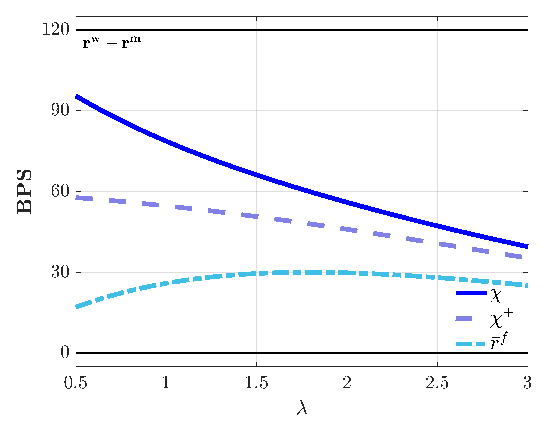
\includegraphics[width=1\linewidth]{NewCode/Figures/F_l_prices_lambda.eps}\end{minipage}\hfill{}  
   \begin{minipage}[b]{.45\linewidth}
   \center{(b) Cobb-Douglas }  \\[4pt]
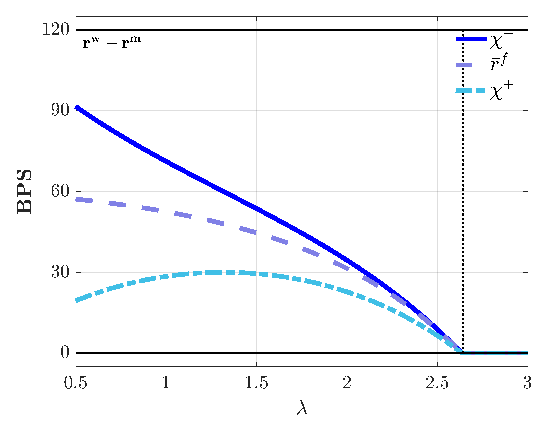
\includegraphics[width=1\linewidth]{NewCode/Figures/F_cd_prices_lambda.eps}
\end{minipage}
\caption{\label{fig:efficiency.compstat} Effects of Matching Efficiency}
\parbox[b]{0.99 \textwidth} {\footnotesize{\emph{Note:}} Rates and Yield Coefficients as functions of $\lambda$ for Leontief
and Cobb-Douglas Matching Functions. Note: The OTC rate and liquidity
yield coefficients are plotted as functions of $\bar{\lambda}$. Both
panels are calibrated using $\eta=0.5$, $\theta_{0}=0.75$, $r^{w}-r^{m}=120$bps.  }
\end{figure}

\FloatBarrier

\paragraph*{OTC Rate Dispersion.}

The dispersion of OTC rates within each trading day---the difference
between rates at the beginning and end of the trading session---provides
another observable moment for parameter identification. Recall from
Proposition \ref{prop:} that the equilibrium rate varies
during the trading session according to market evolution of the tightness
$\theta_{\tau}$. Since rates change monotonically throughout the
day, increasing (decreasing) with time if $\theta>1$ ($\theta<1$),
we can measure dispersion in rates:
\[
Q\equiv \max_{\tau} r^{f}_{\tau} - \min_{\tau} r^{f}_{\tau}=\left|r_{1}^{f}-r_{0}^{f}\right|.
\]
We obtain the following relationship between parameters and the dispersion:

\begin{corollary}
    [Comparative Statics: Rate Dispersion]\label{prop:dispersion.compstats}
Rate dispersion features the following comparative statics:
\begin{enumerate}
\item [i)] If $\theta<0$, then $\frac{\partial Q}{\partial\theta}<0$;
%, with equality if and
%only if $\theta=1$.
\item [ii)] If $\theta>1$, then $\frac{\partial Q}{\partial\theta}>0$;
\item [iii)] If $\theta=1$, then $\frac{\partial Q}{\partial\theta}=0$;
% \item [i)] If $\theta\leq1$ ($\theta\geq1$), then $\frac{\partial Q}{\partial\theta}\leq0$
% ($\frac{\partial Q}{\partial\theta}\geq0$), with equality if and
% only if $\theta=1$.

\item [iv)] $\frac{\partial Q}{\partial\bar{\lambda}}\geq0$ with equality if
and only if $\theta=1$.
\end{enumerate}
\end{corollary}

The intuition is straightforward. Rate dispersion reflects how much
the market \textquotedbl unwinds\textquotedbl{} during the trading
session. When the market is unbalanced ($\theta\not=1$), the scarce
side gets progressively better terms as trading proceeds, creating
larger rate movements. The more unbalanced the market---in either
direction---the greater the dispersion. Similarly, higher matching
efficiency $\bar{\lambda}$ accelerates this unwinding process, amplifying
dispersion. At $\theta=1$, the market is balanced and rates remain
constant throughout the session, yielding $Q=0$.

Figure \ref{fig:dispersion} illustrates these patterns. Panel (a)
shows the symmetric U-shape of dispersion around $\theta=1$ for the,
while panel (b) demonstrates how dispersion increases with matching
efficiency. Panels (c) and (d) show the corresponding mappings for the Cobb-Douglas case, demonstrating that these patterns are robust
across matching technologies. These relationships provide additional
moments for identification: observing both the level of OTC rates
(which pins down $\theta$) and their intraday dispersion $Q$ (which
helps identify $\bar{\lambda}$) can jointly identify OTC market parameters. 

\begin{figure}[htb]
\begin{centering}

\centerline{Leontief Matching}
   \begin{minipage}[b]{.49\linewidth} 
   \center{(a) Varying $\theta$ } \\[4pt]
   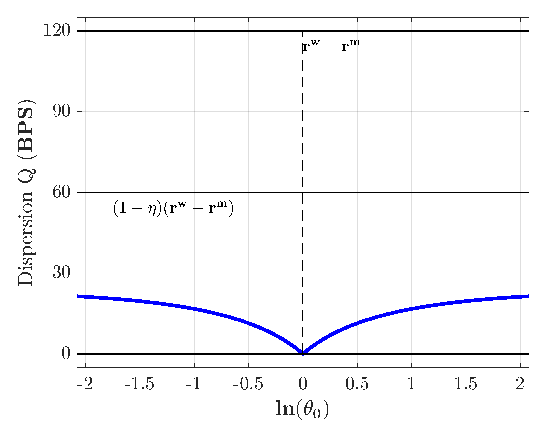
\includegraphics[width=1\linewidth]{NewCode/Figures/F_l_Q_theta.eps}
\end{minipage}
\begin{minipage}[b]{.49\linewidth}
\center{(b) Varying $\lambda$ } \\[4pt]
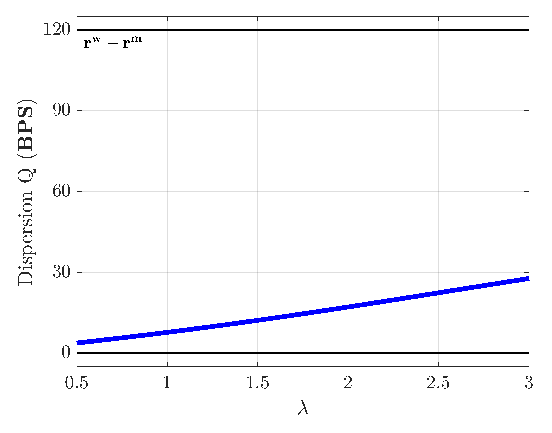
\includegraphics[width=1\linewidth]{NewCode/Figures/F_l_Q_lambda.eps}
\end{minipage}

\vspace{10pt}
\end{centering}

\begin{centering}
\centerline{Cobb-Douglas }
   \begin{minipage}[b]{.49\linewidth} 
\center{(c) Varying $\theta$  } \\[4pt]
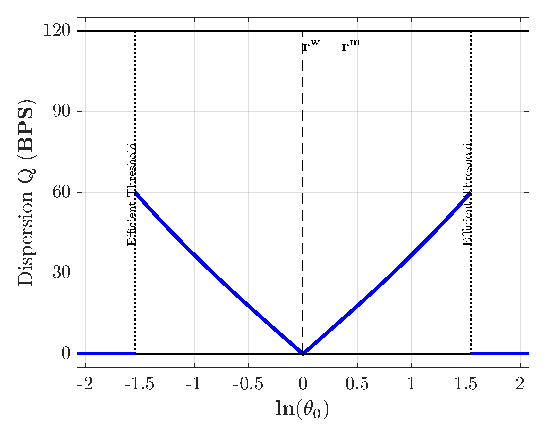
\includegraphics[width=1\linewidth]{NewCode/Figures/F_cd_Q_theta.eps}
\end{minipage}
\begin{minipage}[b]{.49\linewidth}
\center{(d) Varying $\lambda$  } \\[4pt]
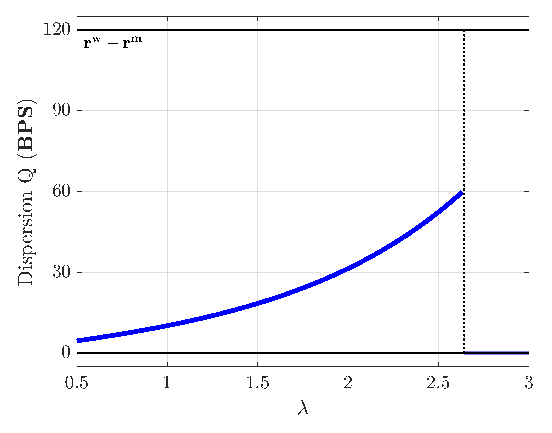
\includegraphics[width=1\linewidth]{NewCode/Figures/F_cd_Q_lambda.eps}
\end{minipage}
\end{centering}
\caption{\label{fig:dispersion}
 Dispersion of OTC Rates as function
of $\left\{ \lambda,\theta_{0}\right\} $.}  

\parbox[b]{0.99 \textwidth} {\footnotesize \emph{Note:} 
The dispersion of
the OTC rate is plotted as a function of $\bar{\lambda}$ and $\theta_{0}$
for the Leontief and Cobb-Douglas matching functions. Both panels
are calibrated using $\eta=0.5$, $r^{w}-r^{m}=120$bps. When we vary
$\bar{\lambda}$, we set $\theta_{0}=0.75$. When we vary $\theta_{0}$
we set $\bar{\lambda}=1.2$.}
\end{figure}

\paragraph*{Relative Volumes of Market and Outside Funding.}

Define the relative volume as the ratio of lender-of-last-resort borrowing
to OTC market borrowing:
\[
I\left(\theta\right)\equiv\frac{1-\Psi^{-}\left(\theta\right)}{\Psi^{-}\left(\theta\right)}=\begin{cases}
\frac{e^{-\bar{\lambda}}}{1-e^{-\bar{\lambda}}} & \theta\leq1\\
\\\frac{1-\left(1-e^{-\bar{\lambda}}\right)\theta^{-1}}{\left(1-e^{-\bar{\lambda}}\right)\theta^{-1}} & \theta>1.
\end{cases}
\]

This ratio captures market efficiency in reallocating liquidity: if
$I\left(\theta\right)=0$ indicates perfect reallocation through the
OTC market whereas $I\left(\theta\right)=\infty$ indicates no OTC
volume at all. We call $I\left(\theta\right)$ the relative volume.

% \begin{proposition}[Comparative Statics: Relative Volume] The relative
% volume features the following comparative statics:
% \begin{enumerate}
% \item [] \emph{Tightness:} The relative volume increases (remains constant)
% with the tightness if $\theta>1$ ($\theta<1$): 
% \[
% \frac{\partial I\left(\theta\right)}{\partial\theta}\frac{\theta}{I\left(\theta\right)}=\frac{\theta}{\theta-1+e^{-\bar{\lambda}}}\mathbb{I}_{\left[\theta>1\right]}\ge0.
% \]
% \item [] \emph{Effiency:} The relative volume increases (remains constant)
% with the tightness if $\theta>1$ ($\theta<1$): 
% \[
% \frac{\partial I\left(\theta\right)}{\partial\bar{\lambda}}\frac{\bar{\lambda}}{I\left(\theta\right)}=-\bar{\lambda}^{2}\left(\frac{e^{-\bar{\lambda}}}{1-e^{-\bar{\lambda}}}+\frac{\left(\theta-1\right)\mathbb{I}_{\left[\theta>1\right]}+1}{e^{-\bar{\lambda}}}\right)<0.
% \]
% \end{enumerate}
% \end{proposition}

These results reveal a key property for identification:
Given Proposition \ref{prob:limit}, the
relative volume
decreases monotonically with matching efficiency $\bar{\lambda}$
regardless of market tightness. This contrasts sharply with convenience
yields, which can be non-monotonic in $\bar{\lambda}$. Moreover,
when markets have excess liquidity $\left(\theta<1\right)$, relative
volume depends only on $\bar{\lambda}$ and is independent of $\theta$
in the Leontief case. Combined with our earlier results, this suggests
that the relative volume is convenient to pin down $\bar{\lambda}$. 

Figure \ref{fig:volume.compstats} illustrates these patterns for
the Leontief case (panels a and b). Panels (c and d) demonstrate a
similar pattern for the Cobb-Douglas case, demonstrating again that
patterns are robust across matching technologies. Notice that in panel c, as the tightness crosses the threshold of efficient trade, indicated by the vertical lines, the relative volume is either zero (when deficits are the short side) or, otherwise, $\frac{S^{-}-S^{+}}{S^{+}}$. Likewise, in panel d, as efficiency crosses a threshold, the relative volume is zero. 

\begin{figure}[H]
\begin{centering}

\centerline{Leontief }
   \begin{minipage}[b]{.49\linewidth}
   \centering
   {(a) Varying $\theta$}  \\[4pt]
   \includegraphics[width=0.8\linewidth]{NewCode/Figures/F_l_vol_theta.eps}
\end{minipage}\hfill   
\begin{minipage}[b]{.49\linewidth}
\center{(b) Varying $\lambda$ }  \\[4pt]
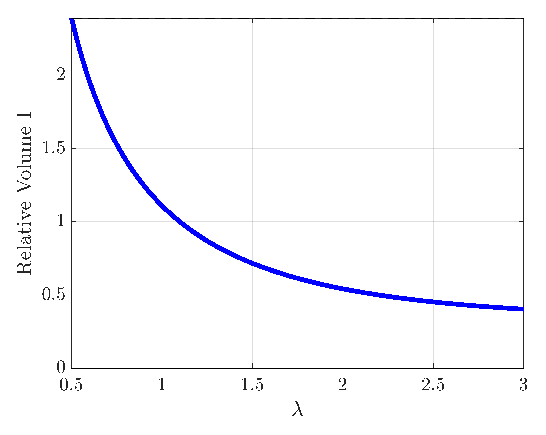
\includegraphics[width=0.8\linewidth]{NewCode/Figures/F_l_Vol_lambda.eps}
\end{minipage}

\vspace{10pt}

\end{centering}

\centerline{Cobb-Douglas }
  \begin{minipage}[b]{.49\linewidth} 
\center{(c) Varying $\theta$}  \\[4pt]
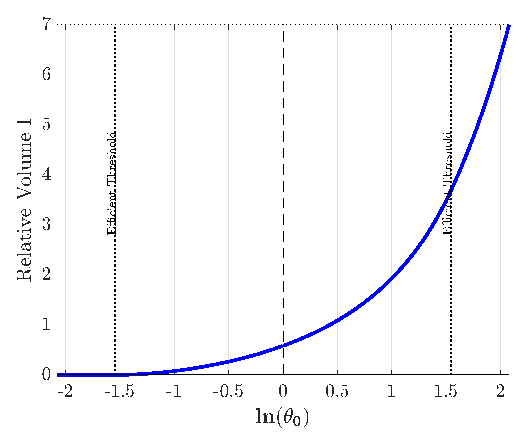
\includegraphics[width=0.8\linewidth]{NewCode/Figures/F_cd_Vol_theta.eps}
\end{minipage}
\begin{minipage}[b]{.49\linewidth}
\center{(d) Varying $\lambda$ }
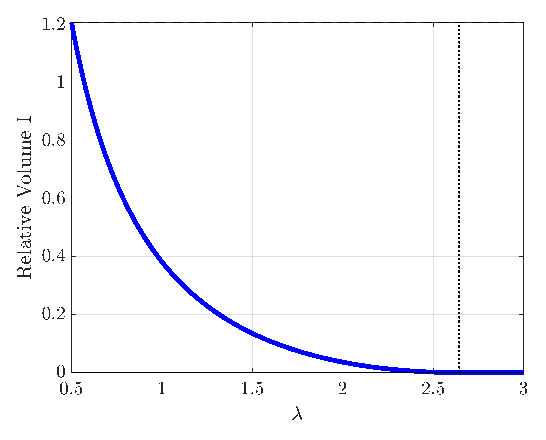
\includegraphics[width=0.8\linewidth]{NewCode/Figures/F_cd_Vol_lambda.eps}
\end{minipage}

\caption{\label{fig:volume.compstats} Relative Volume as Function
of $\left\{ \lambda,\theta_{0}\right\} $.} 

\parbox[b]{0.99 \textwidth} {\footnotesize \emph{Note:} The relative trading
volume is plotted as a function of $\bar{\lambda}$ and $\theta_{0}$
for the Leontief and Cobb-Douglas matching functions. Both panels
are calibrated using $\eta=0.5$, $r^{w}-r^{m}=120$bps. When we vary
$\bar{\lambda}$, we set $\theta_{0}=0.75$. When we vary $\theta_{0}$
we set $\bar{\lambda}=1.2$.}
\end{figure}


\paragraph*{
%Identification Strategy: Putting It All Together.
Summing up.}

Our comparative statics results suggest practical approaches for identifying
the three key parameters of the model $\{\theta,\bar{\lambda},\eta\}$
from observable data. The key insight is to exploit the different
monotonicity properties to achieve robust identification: relative
volume $I(\theta)$ appears to provide a clean first-stage identification
of $\bar{\lambda}$ because it decreases monotonically with matching
efficiency regardless of market conditions. Once $\bar{\lambda}$
is pinned down, the monotonic relationship between convenience yields
and $\theta$ allows for second-stage identification. Crucially, since
$\theta$ depends on both portfolios and the distribution of settlement
shocks, observing portfolios allows us to infer the unobservable shock
distribution $\Phi$.

For empirical work, this framework suggests focusing data collection
on: (i) portfolio compositions across institutions, (ii) spreads between
liquid and illiquid assets, (iii) the level and intraday range of
OTC rates, and (iv) the relative use of emergency lending facilities,
if available. Together, these moments may sufficiently identify both the market microstructure driving convenience yields and the underlying
distribution of liquidity shocks. We provide a sketch of an identification
strategy next.

\begin{algorithm*}[htb]
\caption{Suggested Identification Approach}
\vspace{10pt}
\begin{algorithmic}
\STATE \textbf{Given possible observable data:}
\STATE \quad - Portfolio holdings across investors, $\{m,a^i\}$, convenience yields on liquid assets: $R^b - R^m$, an average OTC rate: $\bar{r}^f$, rate dispersion: $Q = |r^f_1 - r^f_0|$,  relative volume: $I$
\STATE
\STATE \textbf{Step 1: Identify matching efficiency $\bar{\lambda}$}
\STATE \quad -Use $I(\theta)$ to infer $\bar{\lambda}$ (monotonic for all $\theta$)
\STATE
\STATE \textbf{Step 2: Identify market tightness $\theta$ and shock distribution $\Phi$}
\STATE \quad -Given $\bar{\lambda}$ from Step 1:
\STATE \quad -Use convenience yields or $\bar{r}^f$ to infer $\theta$  
\STATE \quad -Given observed portfolios and implied $\theta$, back out the distribution $\Phi$ of shocks (e.g., withdrawal risk parameters)
\STATE
\STATE \textbf{Step 3: Identify bargaining power $\eta$}
\STATE \quad -Consider the historical average of $\bar{r}^f$ relative to $r^m$ and $r^w$
\STATE \quad or examine the ratio $\chi^+/\chi^-$ near balanced markets
\STATE
\STATE \textbf{Step 4: Validation}
\STATE \quad - Check implied $Q(\theta,\bar{\lambda})$ aligns with observed dispersion
\STATE \quad - Assess consistency across different liquid assets
\end{algorithmic}
\end{algorithm*}

\FloatBarrier 
\subsection{Normative Analysis}

In this section, we study the implications of the theory for liquidity regulation. We do so by comparing the decentralized portfolio choices vis-à-vis a social planner's portfolio choices. The goal is to analyze externalities among investors, in isolation
from the effects on supply and demand effects on assets nor the revenues of the lender of last resort. Potential inefficiencies arise because portfolio decisions affect the tightness in the OTC market, inducing possible congestion externalities. In particular, when the planner chooses a higher level of liquid assets, this increases the likelihood
that an investor in deficit will be able to match. Conversely, if the planner chooses a lower level of liquid assets, it increases the likelihood
of a surplus investor finding a match. Moreover, as we show below, the fact that the convenience yield is asymmetric implies that risk aversion plays an important role, as the amount of aggregate liquidity
affects the degree of risk faced by investors.

To illustrate the externality,  consider a simple example. We specialize the model to the case where investors' portfolios are composed of a liquid asset 
$m$, an illiquid asset $b$, and deposits
$d$. In particular, deposits are subject to withdrawal risk such that \eqref{eq:surplus} is given by
\begin{equation}
s\left(\left\{ b,d\right\} ,m\right)\equiv m+\left(\frac{R^{d}}{R^{m}}\omega-\rho(1+\omega)\right)d,\label{eq:withdrawalexample.cash}
\end{equation}
and their budget constraint is: $b+m=1+d$ where $\omega$ is distributed
$F$ with mean zero. 

We study the individual investor's problem next and then consider the planner's counterpart.

\paragraph{Investor's problem}
The investor's problem, after substituting its
budget constraint, thus becomes:

\begin{problem}[Withdrawal Risk Problem]The investor's problem in
example is:
\[
\max_{m\ge0,d\geq0}\left\{ \mathbb{E}_{\omega}\left[R^{b}+R^{b}(d-m)+\ R^{m}m-\ R^{d}d+\chi\left(s\left(d,m\right);\theta\right)\right]^{1-\gamma}\right\} ^{\frac{1}{^{1-\gamma}}},
\]

\end{problem}

In this simple example, the optimality condition (\ref{eq:liquidity.premiumcov}),
is simple and links the portfolio to a convenience yield, a spread,
between illiquid assets and cash:

\begin{equation}
\underbrace{R^{b}-R^{m}}_{\text{liquidity premium}}=\chi^{+}\left(1-\tilde{\Phi}\left(\omega^{\ast}\right)\right)+\chi^{-}\tilde{\Phi}\left(\omega^{\ast}\right)=\chi^{+}+\Sigma\left(\theta\right)\tilde{\Phi}\left(\omega^{\ast}\right)\cdot\label{eq:illiquidbond.premium}
\end{equation}
where 
\[
\tilde{\Phi}\left(\omega^{\ast}\right)=\underbrace{\underset{\text{deficit prob}}{\underbrace{\Phi\left(\omega^{\ast}\right)}}\cdot\underset{\text{risk-aversion correction}}{\underbrace{\frac{\mathbb{E}_{\omega}\left[R^{e}(\omega)^{-\gamma}|\omega<\omega^{\ast}\right]}{\mathbb{E}_{\omega}\left[R^{e}(\omega)^{-\gamma}\right]}}}}_{\text{risk-adjusted deficit probability}},\quad\omega^{\ast}\equiv\frac{\rho-\dfrac{m}{d}}{\dfrac{R^{d}}{R^{m}}-\rho}.
\]

Thus, the liquidity premium is a weighted average of the liquidity
yield coefficients, $\chi^{+}\left(1-\tilde{\Phi}\left(\omega^{\ast}\right)\right)+\chi^{-}\tilde{\Phi}\left(\omega^{\ast}\right)$.
In the expression, $\tilde{\Phi}\left(\omega^{\ast}\right)$ is the
risk-adjusted probability of falling in a cash deficit.\footnote{The risk adjustment scales probabilities by marginal utilities of
wealth.} The probability of a deficit is $\Phi\left(\omega^{\ast}\right)$
where $\omega^{\ast}$ is the threshold shock that puts banks in deficit---recall
that lower values of $\omega$ represent an outflow of funds. Thus,
the liquidity premium of cash over illiquid assets is their risk-adjusted
expected return of coming into the OTC market with an extra unit
of cash.

In the special case of risk-neutrality, we have that (\ref{eq:illiquidbond.premium})
becomes:
\[
\underbrace{R^{b}-R^{m}}_{\text{liquidity premium}}=\chi^{+}+\left(R^{w}-R^{m}\right)\left(1-\Psi^{-}\left(\theta\right)\right)\Phi\left(\omega^{\ast}\right).
\]
The corresponding difference between illiquid assets and deposits is
an interest margin associated with the liquidity risk of deposits:
\begin{equation}
\underbrace{R^{b}-R^{d}}_{\text{liquidity premium}}=\chi^{+}+\left(\chi^{-}-\chi^{+}\right)\tilde{\Phi}\left(\omega^{\ast}\right)\left(\left(\frac{R^{d}}{R^{m}}-\rho\right)\mathbb{E}_{\omega}\left[\omega R^{e}(\omega)^{-\gamma}|\omega<\omega^{\ast}\right]-\rho\right)\cdot\label{eq:deposit.premium}
\end{equation}
When deposits are riskier, as captured by the left tail of the distribution, this requires a higher return on loans. 

Next, we discuss how features of the OTC market affect the liquidity
yield coefficients and, consequently, the return premia. In turn,
we discuss how OTC market frictions can be inferred from convenience
yields or OTC market data to discipline the theory.

\paragraph{Constrained efficient allocation.}
We assume the planner chooses the portfolio shares $(d,b,m)$ on behalf of investors while investors retain the choice of how much to save overall and how much to consume. The planner takes as given all portfolio returns and the structure of the OTC market, as encoded in the convenience yield function. 

\begin{problem}The planner's problem is:
\[
\max_{m\ge0,d\geq0}\left\{ \mathbb{E}_{\omega}\left[R^{b}(d-m)+\ R^{m}m-\ R^{d}d+\chi\left(s\left(\omega,m,d\right),\theta(m,d)\right)\right]^{1-\gamma}\right\} ^{\frac{1}{^{1-\gamma}}},
\]
subject to \eqref{eq:withdrawalexample.cash} and the market tightness
\[
\theta\left(m,d\right)\equiv\frac{\int_{-1}^{\omega^{\ast}}s\left(\omega,m,d\right)\Phi^ {}(d\omega)}{\int_{\omega^{\ast}}^{\infty}s\left(\omega,m,d\right)\Phi(d\omega)},\quad\omega^{\ast}\equiv\frac{\rho-\dfrac{m}{d}}{\dfrac{R^{d}}{R^{m}}-\rho}.
\]

\end{problem}

The key distinction is that the planner considers how the portfolio
determines $\theta$ and how in turn this affects the convenience
yield function $\chi$. Notice that because all investors are identical ex ante, there are no redistribution considerations.


The planner's first-order conditions with
respect to $m$ and $b$ yields the following first-order condition:
\begin{multline}
\underbrace{R^{b}-R^{m}}_{\text{asset premium}}=\chi^{+}+\left(\chi^{-}-\chi^{+}\right)\cdot\tilde{\Phi}\left(\omega^{\ast}\right) + \\ 
\frac{\partial\theta}{\partial m}\frac{\partial\chi^{+}(\theta)}{\partial\theta}\cdot(1-\tilde{\Phi}(\omega^{\ast}))\cdot\mathbb{E}\left[s\cdot\frac{R^{e}(\omega)^{-\gamma}}{\mathbb{E}\left[R^{e}(\omega)^{-\gamma}\middle|\;\omega>\omega^{\ast}\right]}|\;\omega>\omega^{\ast}\right]\\[4pt]
  +\frac{\partial\theta}{\partial m}\frac{\partial\chi^{-}(\theta)}{\partial\theta}\cdot\tilde{\Phi}(\omega^{\ast})\cdot\mathbb{E}\left[s\cdot\frac{R^{e}(\omega)^{-\gamma}}{\mathbb{E}\left[R^{e}(\omega)^{-\gamma}\middle|\;\omega<\omega^{\ast}\right]}|\;\omega<\omega^{\ast}\right].
\end{multline}
Just like individual investors, the planner trades off the higher return on loans with the liquidity benefits of cash, considering the uses of cash in the OTC market. However, the planner internalizes the pecuniary externality that emerges because it understands how portfolio choices will affect trading probabilities, as encoded in the convenience yield $\chi$. 

A key insight is that the sign of the externality is ambiguous: it depends on the derivatives of the convenience-yield coefficients.  To understand whether investors over- or under-invest in liquid assets, it is useful to consider first the limiting case with risk-neutral investors. With $\gamma\rightarrow0$, given that $\frac{\partial\theta}{\partial m}<0,\frac{\partial\chi^{+}(\theta)}{\partial\theta}>0,\frac{\partial\chi^{-}(\theta)}{\partial\theta}>0,$
we have that the \textit{planner values cash more} than individual
investors if and only if
\begin{equation}
\frac{\partial\chi^{+}(\theta)}{\partial\theta}\cdot S^{+}>\frac{\partial\chi^{-}(\theta)}{\partial\theta}\cdot S^{-}
\end{equation}
This inequality underscores that there is an under-accumulation of liquid assets when the planner perceives that higher cash holdings (lower market tightness) raise the marginal return on liquid  assets more when in deficit, compared to the case in surplus. That is, when market tightness goes up, this favors investors that are in deficit  (by allowing them to borrow at a lower rate and by raising the probability of a match) relative to investors that are in surplus (as they now must lend at a lower rate and face a lower matching probability).

Suppose that the planner picks a portfolio with $\theta=1$. Under
the case with Cobb-Douglas matching, we know that $\frac{\partial\chi^{+}(\theta)}{\partial\theta}=\frac{\partial\chi^{-}(\theta)}{\partial\theta}$.
If, in addition, the shock is symmetric $F(\omega^{\ast})=0.5$ and $\mathbb{E}\left[-s\mid\omega<\omega^{\ast}\right]=\mathbb{E}\left[s\mid\omega\ge\omega^{\ast}\right]$.\footnote{To see that $\frac{\partial\chi^{+}(\theta)}{\partial\theta}|_{\theta=1}=\frac{\partial\chi^{-}(\theta)}{\partial\theta}|_{\theta=1}$
under Cobb-Douglas we can exploit the symmetry property of derivatives.} In this case, it follows that there is neither over- nor under-accumulation
of liquid assets. However, if investors were risk-averse, the risk adjustment correction would imply that by accumulating more liquid
assets, the planner would effectively provide more insurance. Because individual investors do not internalize these benefits, the competitive
equilibrium would feature under-accumulation of liquid assets. In addition, 
an allocation with a higher probability of being in deficit $\Phi(\omega^{\ast})$
or with a more sensitive convenience yield$\frac{\partial\chi^{-}(\theta)}{\partial\theta}$
implies that the planner perceives a higher value from higher liquid holdings.

It is also interesting to discuss the case with Leontief matching. In this case, while matching probabilities do not change
with market tightness on the short-side of the market at the margin,
aggregate cash holdings affect endogenously the outside options of
investors, the OTC rate does change, and so does $\chi^{+}$ and $\chi^{-}.$
Notice that if the OTC market were static, the OTC rate would be fixed, and so in this case, it would suffice to know whether the market features excess surplus or deficit to trace the sign of the inefficiency,  under risk neutrality. In particular, if the market had, on average,
excess surplus, the planner would value less cash than individual investors at the margin. Conversely, if the market had, on average, excess deficits, the planner would value more cash than individual
investors at the margin. This follows because in the former case $\frac{\partial\chi^{-}(\theta)}{\partial\theta}=0$
and $\frac{\partial\chi^{+}(\theta)}{\partial\theta}>0$ while in
the latter $\frac{\partial\chi^{+}(\theta)}{\partial\theta}=0$ and
$\frac{\partial\chi^{-}(\theta)}{\partial\theta}>0.$

This externality has direct implications for prudential policy. Suppose a planner’s objective is to minimize reliance on penalty borrowing—as in open-economy settings where institutions hold foreign reserves but must borrow from external lenders at a penalty rate. Our results show that achieving this objective may require either encouraging or discouraging liquidity holdings, depending on the market environment, in order to reduce external borrowing costs. \footnote{\citet{ismailWelfareCostConvenience2025} study the converse problem, where the planner internalizes the revenues from penalty borrowing (because it operates the discount window) and rebates them back to banks. In contrast, their analysis focuses on the welfare implications from an asset-demand perspective, i.e., the wedge between loan and deposit rates.}

%---------------------------
 \section{Conclusions}

 \label{sec:conclusions}
We develop a tractable microfoundation for convenience yields arising from trading frictions in OTC markets for settlement instruments and show how it can be readily introduced into a canonical portfolio problem. We further characterize how the convenience yield function depends on market tightness, bargaining power, and matching efficiency, and show that convenience yields reflect both direct OTC frictions and the interaction between liquidity and return risk. The framework generates closed-form expressions for rates and spreads that facilitate comparative statics and quantitative analysis.  Finally, we show that individual investors fail to internalize how their portfolio choices influence aggregate market tightness, which leads to over- or under-investment in liquid assets depending on the level of tightness and the degree of risk aversion.

Our framework abstracts from several important features of real-world markets that offer fertile ground for future work. First, the model lacks large market makers, whose balance sheet constraints can impair the functioning of OTC markets. Second, we omit the role of collateral, which may shape both the terms and scope of OTC trades. Third, we consider a single-layer liquidity environment. In contrast, in practice, liquidity provision is organized through a multi-layered architecture: central banks backstop banks through lending facilities, and their liabilities serve as the settlement instrument among banks; banks, in turn, provide credit lines and deposits that serve as settlement instruments for non-bank financial institutions. These interlocking layers of settlements and liquidity provision imply that frictions at one level can propagate throughout the system. Equipped with suitable data to infer its parameter, our framework can contribute to a deeper understanding of the determinants of convenience yields and of asset pricing more broadly.

\newpage{}


\let\OLDthebibliography\thebibliography
\renewcommand\thebibliography[1]{
  \OLDthebibliography{#1}
  \setlength{\parskip}{0.5pt}
  \setlength{\itemsep}{0pt plus 0.3ex}
}
% \nocite{afonso2015over}\bibliographystyle{aer}
\bibliography{bib_interbank}

\newpage{}

\thispagestyle{empty}
\appendix

% \pagenumbering{arabic} 
% \appendix

\setcounter{page}{1}

\renewcommand{\thepage}{A\arabic{page}}

\clearpage{\huge Appendix (not intended for publication)}{\huge\par}


\clearpage

\appendixtoc        % Print the TOC
\startappendixtoc   % Activate TOC tracking

\newpage{}

\section{Proof of Proposition \ref{P_LimitingRates}}

\renewcommand{\theequation}{A.\arabic{equation}}
\setcounter{equation}{0}
\renewcommand{\thedefinition}{A.\arabic{definition}}
\setcounter{definition}{0}

We begin with an auxiliary Lemma showing that market tightness follows a difference equation. With the market tightness, we obtain the matching probabilities at each round:

\begin{lemma}\label{lem:C_Continuities}
Let $\theta_{0}$ be the initial market tightness. Then,
the ratio $\left\{ \theta_{n}\right\}$ features the following law
of motion: 
\[
\theta_{n}=\theta_{n-1}\frac{\left(1-\lambda_{N}G\left(1/\theta_{n-1},1\right)\right)}{\left(1-\lambda_{N}G\left(1,\theta_{n-1}\right)\right)}\,\qquad\forall n\in\{1,2,\dots,N\}.
\]
and the matching probabilities can be expressed in terms of the ratio
via:
\[
\psi_{n}^{+}=\lambda_{N}G\left(1,\theta_{n-1}\right)\text{ and }\psi_{n}^{-}=\lambda_{N}G\left(1/\theta_{n-1},1\right).
\]
\end{lemma}

\begin{proof}
By definition and homogeneity:
\[
\theta_{n}=\frac{S_{n}^{-}}{S_{n}^{+}}=\frac{S_{n-1}^{-}-z_{n}}{S_{n-1}^{+}-z_{n}}=\theta_{n-1}\frac{\left(1-\lambda_{N}G\left(1/\theta_{n-1},1\right)\right)}{\left(1-\lambda_{N}G\left(1,\theta_{n-1}\right)\right)},\qquad\forall n\in\{1,2,\dots,N\}.
\]
where the second equality follow from the definition of $z_{n}$ and
uses its homogeneity property.
\end{proof}

The lemma shows that we can track matching probabilities
in terms of the initial market tightness, without reference to the terms of trade. It also shows that the these probabilities are scale invariant. We use these observations in what follows, as the Lemma permits us to treat trading probabilities as exogenous series.

The proof also makes use of the following standard result in probability, which we include for ease of completeness:
\begin{lemma}[Conditional Probability Decomposition]
\label{lem:appendix.condprobs}
For any starting round $n \geq 0$, the conditional probabilities of matching satisfy:
\[
\sum_{k=n+1}^{N} \psi_{k}^{\pm}\prod_{m=n+1}^{k-1}(1-\psi_{m}^{\pm}) + \prod_{m=n+1}^{N}(1-\psi_{m}^{\pm}) = 1
\]
That is, starting from round $n$, the probability of matching in some future round plus the probability of never matching equals 1.
\end{lemma}

\begin{proof}
Let $P_{n,j} = \prod_{m=n+1}^{j}(1-\psi_{m}^{\pm})$ be the probability of not matching from round $n+1$ through round $j$, with the convention that $P_{n,n} = 1$.

Then:
\begin{align*}
\sum_{k=n+1}^{N} \psi_{k}^{\pm}\prod_{m=n+1}^{k-1}(1-\psi_{m}^{\pm}) &= \sum_{k=n+1}^{N} \psi_{k}^{\pm} P_{n,k-1}\\
&= \sum_{k=n+1}^{N} [P_{n,k-1} - P_{n,k}] \quad \text{(since } P_{n,k} = P_{n,k-1}(1-\psi_k^{\pm})\text{)}\\
&= (P_{n,n} - P_{n,n+1}) + (P_{n,n+1} - P_{n,n+2}) + \cdots + (P_{n,N-1} - P_{n,N})\\
&= P_{n,n} - P_{n,N}\\
&= 1 - \prod_{m=n+1}^{N}(1-\psi_{m}^{\pm})
\end{align*}
where we used $P_{n,n} = 1$ and the telescoping sum. The result follows by rearranging.
\end{proof}

Next, we describe the limit of the bargaining problem
as $\Delta\rightarrow0$. Recall that the trader's estimate of equity, excluding its own trade, is:
\[
\mathcal{E}^{j}(\Delta) \equiv \sum_{i\in\mathbb{I}}a_{t+1}^{i}R_{t+1}^{i}+m_{t+1}R_{t+1}^{m}+\chi_{t+1}(s^{j}-\sign\{s^{j}\}\Delta).
\]
The proof of Proposition \ref{P_LimitingRates} is as follows:
\begin{proof}
The Nash bargaining problem at round $n$ with trade size $\Delta$ has surplus for trader with position $s^j$:
\[
\mathcal{S}_n^{\text{sign}\{s^j\}}(\Delta) = V(\mathcal{E}^j(\Delta) + \text{sign}\{s^j\}(r_n^f - r^m)\Delta) - J_U^{\text{sign}\{s^j\}}(n;\Delta).
\]

\textbf{Step 1: Outside option recursion.} The unmatched value satisfies:
\[
J_U^{\text{sign}\{s^j\}}(n;\Delta) = \psi_{n+1}^{\text{sign}\{s^j\}} V(\mathcal{E}^j(\Delta) + \text{sign}\{s^j\}(r_{n+1}^f - r^m)\Delta) + (1-\psi_{n+1}^{\text{sign}\{s^j\}})J_U^{\text{sign}\{s^j\}}(n+1;\Delta),
\]
with terminal round, $N$, values given by:
\begin{align*}
J_U^{+}(N;\Delta) &= V(\mathcal{E}^j(\Delta)) \quad \text{(surplus traders hold cash at rate } r^m\text{)}\\
J_U^{-}(N;\Delta) &= V(\mathcal{E}^j(\Delta) - (r^w - r^m)\Delta) \quad \text{(deficit traders borrow at rate } r^w\text{)}.
\end{align*}

Expanding the recursion forward from round $n$:
\begin{align*}
J_U^{\text{sign}\{s^j\}}(n;\Delta) = &\sum_{k=n+1}^{N} \left[\prod_{m=n+1}^{k-1}(1-\psi_m^{\text{sign}\{s^j\}})\right]\psi_k^{\text{sign}\{s^j\}} V(\mathcal{E}^j(\Delta) + \text{sign}\{s^j\}(r_k^f - r^m)\Delta)\\
&+ \left[\prod_{m=n+1}^{N}(1-\psi_m^{\text{sign}\{s^j\}})\right] V(\mathcal{E}^j(\Delta) + \text{sign}\{s^j\}\chi_{N+1}^{\text{sign}\{s^j\}}\Delta).
\end{align*}
By Lemma \ref{lem:appendix.condprobs}, this corresponding to the value of $\mathbb{E}\left[ V(\mathcal{E}^j(\Delta) + \text{sign}\{s^j\} (r^f_n - r^m)\Delta)|\text{unmatched by n} \right].$ Importantly, notice that the expectation assumes that the negotiated rated in future rounds $r^f_n$ only depends on future rounds, an assumption that we have to verify below.

Now, consider the normalized difference::
\begin{align*}
\frac{J_U^{\text{sign}\{s^j\}}(n;\Delta) - V(\mathcal{E}^j(\Delta))}{\Delta} = &\sum_{k=n+1}^{N} \left[\prod_{m=n+1}^{k-1}(1-\psi_m^{\text{sign}\{s^j\}})\right]\psi_k^{\text{sign}\{s^j\}} \frac{V(\mathcal{E}^j + \text{sign}\{s^j\}(r_k^f - r^m)\Delta) - V(\mathcal{E}^j)}{\Delta}\\
&+ \left[\prod_{m=n+1}^{N}(1-\psi_m^{\text{sign}\{s^j\}})\right] \frac{V(\mathcal{E}^j + \text{sign}\{s^j\}\chi_{N+1}^{\text{sign}\{s^j\}}\Delta) - V(\mathcal{E}^j)}{\Delta}.
\end{align*}

As $\Delta \to 0$, by the definition of derivative:
\[
\lim_{\Delta \to 0} \frac{J_U^{\text{sign}\{s^j\}}(n;\Delta) - V(\mathcal{E}^j(\Delta))}{\Delta} = \text{sign}\{s^j\} \cdot V'(\mathcal{E}^j) \cdot \chi_n^{\text{sign}\{s^j\}}
\]
where:
\begin{equation}
\label{eq:appendix.recursion}
\chi_n^{\text{sign}\{s^j\}} = \sum_{k=n+1}^{N} (r_k^f - r^m)\left[\prod_{m=n+1}^{k-1}(1-\psi_m^{\text{sign}\{s^j\}})\right]\psi_k^{\text{sign}\{s^j\}} + \chi_{N+1}^{\text{sign}\{s^j\}}\prod_{m=n+1}^{N}(1-\psi_m^{\text{sign}\{s^j\}}).
\end{equation}
The variable $\chi_n^{\text{sign}\{s^j\}}$ represents the expected financing cost/benefit conditional on being unmatched at round $n$, for $+$ and $-$ positions. The variables satisfy the following recursion:
\begin{equation}
\chi_n^{\text{sign}\{s^j\}} = \psi_{n+1}^{\text{sign}\{s^j\}}(r_{n+1}^f - r^m) + (1-\psi_{n+1}^{\text{sign}\{s^j\}})\chi_{n+1}^{\text{sign}\{s^j\}}
\label{eq:chi-recursion}
\end{equation}
with terminal conditions $\chi_{N+1}^{+} = 0$ and $\chi_{N+1}^{-} = r^w - r^m$.

\textbf{Step 2: Limiting surplus.} Consider the following term:
\begin{equation*}
\frac{S_n^{\text{sign}\{s^j\}}(\Delta)}{\Delta} = \frac{\left(V(\mathcal{E}^j(\Delta) + \text{sign}\{s^j\}(r_n^f - r^m)\Delta) - V(\mathcal{E}^j(\Delta)\right) - \left(J_U^{\text{sign}\{s^j\}}(n;\Delta) - V(\mathcal{E}^j(\Delta))\right)}{\Delta}.
\end{equation*}
Taking the $\Delta \to 0$ limit and substituting the result in Step 1:
\[\lim_{\Delta \to 0} \frac{\mathcal{S}_n^{\text{sign}\{s^j\}}(\Delta)}{\Delta} = \text{sign}\{s^j\}V'(\mathcal{E}^j(0))[(r_n^f - r^m) - \chi_n^{\text{sign}\{s^j\}}].\]

\textbf{Step 3: Nash bargaining.} The bargained rate solves:
\[r_n^f(\Delta) = \arg\max_{r_n} [S_n^{-}(\Delta)]^{\eta}[S_n^{+}(\Delta)]^{1-\eta}.\]
Since multiplying the objective by a positive constant $\Delta^{-1}$ doesn't change the maximizer:
\[r_n^f(\Delta) = \arg\max_{r_n} \frac{[S_n^{-}(\Delta)]^{\eta}[S_n^{+}(\Delta)]^{1-\eta}}{\Delta}= \arg\max_{r_n} \left[\frac{S_n^{-}(\Delta)}{\Delta}\right]^{\eta}\left[\frac{S_n^{+}(\Delta)}{\Delta}\right]^{1-\eta}.\]
Taking the limit as $\Delta \to 0$:
\[r_n^f = \lim_{\Delta \to 0} r_n^f(\Delta) = \lim_{\Delta \to 0} \left\{\arg\max_{r_n} \left[\frac{S_n^{-}(\Delta)}{\Delta}\right]^{\eta}\left[\frac{S_n^{+}(\Delta)}{\Delta}\right]^{1-\eta}\right\}.\]
By the Theorem of the Maximum, since the objective function is continuous in both $r_n$ and $\Delta$, and the constraint set $[r^m, r^w]$ we can pass limits inside the maximum operator:
\[\lim_{\Delta \to 0}r_n^f = \arg\max_{r_n} \left\{\lim_{\Delta \to 0}\left[\frac{S_n^{-}(\Delta)}{\Delta}\right]^{\eta}\left[\frac{S_n^{+}(\Delta)}{\Delta}\right]^{1-\eta}\right\}.\]
Substituting the limits from Step 2:
\[r_n^f = \arg\max_{r_n} \left\{[V'(\mathcal{E}^j(0))]^{\eta}[V'(\mathcal{E}^k(0))]^{1-\eta} \cdot [\chi_n^{-} - (r_n - r^m)]^{\eta}[(r_n - r^m) - \chi_n^{+}]^{1-\eta}\right\}.\]
Since $V'(\mathcal{E}^j(0))$ and $V'(\mathcal{E}^k(0))$ are positive constants independent of $r_n^f$, this reduces to Problem~\ref{prob:limit}:
\[r_n^f = \arg\max_{r_n} [\chi_n^{-} - (r_n - r^m)]^{\eta}[(r_n - r^m) - \chi_n^{+}]^{1-\eta}.\]
where $\chi_n^{+}$ and $\chi_n^{-}$ satisfy \ref{eq:appendix.recursion}. 

\textbf{Step 4: First-order condition.} We now solve the maximization problem. The FOC yields: $\eta[(r_n^f - r^m) - \chi_n^{+}] = (1-\eta)[\chi_n^{-} - (r_n^f - r^m)].$
Therefore: 
\[
r_n^f = r^m + (1-\eta)\chi_n^{-} + \eta\chi_n^{+},
\] 
as stated by the proposition. This justifies the assumption that outside options only consider rates that depend on rates without the need to consider counterparties. 
\end{proof}

\section{Proof of Proposition \ref{P_Consistency}}

\begin{proof}
The matching probabilities over $N$ rounds are:
\[
\Psi^{+} = 1-\prod_{n=1}^{N}(1-\psi_{n}^{+}) \quad \text{and} \quad \Psi^{-} = 1-\prod_{n=1}^{N}(1-\psi_{n}^{-}).
\]
These represent the probability of matching at least once during the OTC stage.

\textbf{Verification of $\chi^+$ and $\chi^-$.} From Proposition~\ref{P_LimitingRates} we obtain the recursion \eqref{eq:appendix.recursion}. Solving that recursion forward, from round $0$ to round $N$:
\begin{equation}
\label{eq:appendix.recursion.expanded}
\chi_{0}^{\pm} = \sum_{n=1}^{N} (r_{n}^{f} - r^{m})\psi_{n}^{\pm}\prod_{k=1}^{n-1}(1-\psi_{k}^{\pm}) + \chi_{N+1}^{\pm}\prod_{n=1}^{N}(1-\psi_{n}^{\pm}).
\end{equation}
where we used $\chi_{N+1}^{+} = 0$ and $\chi_{N+1}^{-} = r^{w} - r^{m}$.
The first term is the OTC rates weighted by the unconditional matching probabilities, and the second term is the terminal value weighted by the probability of never matching ($1-\Psi^{\pm}$). 

Recall that probabilities in the expansion add up to 1: apply Lemma \ref{lem:appendix.condprobs} to $n=1$. Thus, we can define the volume-weighted average rate as:
\[
\overline{r}^{f} -r^{m} =   \sum_{n=1}^{N} (r_{n}^{f} - r^{m})\frac{\psi_{n}^{\pm}\prod_{k=1}^{n-1}(1-\psi_{k}^{\pm})}{\Psi^{\pm}},
\] where the weights in the sum add up to 1. 

Substituting the definition of weighted rates in \eqref{eq:appendix.recursion.expanded}, we obtain:
\begin{align*}
\chi_{0}^{+} &= \Psi^{+}(\overline{r}^{f} - r^{m}) + 0 \cdot (1-\Psi^{+}) = \Psi^{+}(\overline{r}^{f} - r^{m}) = \chi^{+}\\
\chi_{0}^{-} &= \Psi^{-}(\overline{r}^{f} - r^{m}) + (r^{w} - r^{m})(1-\Psi^{-}) = \chi^{-}.
\end{align*}

\paragraph{Consistency of weights.}
Probabilities are proportional to traded amounts since $z_n=\psi_n^{\pm}S^{\pm}_{n-1}$ and $S^{\pm}_{n-1}=\prod_{k=1}^{n-1}(1-\psi_{k}^{\pm})S^{\pm}_{0}$ and $\sum_{n=1}^{N}z_n=\Psi^{\pm}S^{\pm}_{0}.$ Thus, the weights $\varkappa_{n}^{\pm} = \frac{\psi_{n}^{\pm}\prod_{k=1}^{n-1}(1-\psi_{k}^{\pm})}{\Psi^{\pm}}$ are identical for surplus and deficit sides due to the homogeneity of the matching function (see Lemma~\ref{lem:C_Continuities}), ensuring a unique $\overline{r}^{f}$. 
\end{proof}

\section{Proof of Lemma \ref{P_ContinuousProbabilities}}


Consider the continuous-time limit as $N \to \infty$. Let $\Delta = 1/N$ denote the time between rounds, and index continuous time by $\tau \in [0,1]$. We derive the ODE in the statement of the Lemma.

\begin{proof}


\textbf{Step 1: Evolution of masses.} In discrete time, the masses of surplus and deficit positions evolve as:
\[
S_{n+1}^{\pm} = S_n^{\pm} - \lambda_N G(S_n^{+}, S_n^{-}).
\]
With $\lambda_N = \bar{\lambda}/N$ and continuous time $\tau = n/N$, taking $\Delta \to 0$:
\[
\dot{S}_{\tau}^{\pm} = \lim_{\Delta \to 0} \frac{S_{\tau+\Delta}^{\pm} - S_{\tau}^{\pm}}{\Delta} = -\bar{\lambda}G(S_{\tau}^{+}, S_{\tau}^{-}).
\]
Both sides shrink at the same absolute rate since matches clear equal amounts from each side.

\textbf{Step 2: Dynamics of tightness.} Define $\theta_{\tau} = S_{\tau}^{-}/S_{\tau}^{+}$. Taking logarithms and differentiating:
\begin{align*}
\frac{\dot{\theta}_{\tau}}{\theta_{\tau}} &= \frac{d}{d\tau}\ln(\theta_{\tau}) = \frac{d}{d\tau}[\ln(S_{\tau}^{-}) - \ln(S_{\tau}^{+})]\\
&= \frac{\dot{S}_{\tau}^{-}}{S_{\tau}^{-}} - \frac{\dot{S}_{\tau}^{+}}{S_{\tau}^{+}}\\
&= -\bar{\lambda}\frac{G(S_{\tau}^{+}, S_{\tau}^{-})}{S_{\tau}^{-}} + \bar{\lambda}\frac{G(S_{\tau}^{+}, S_{\tau}^{-})}{S_{\tau}^{+}}.
\end{align*}
Using homogeneity of degree one: $G(S^+, S^-) = S^+ G(1, \theta) = S^- G(\theta^{-1}, 1).$
Therefore:
\[
\frac{\dot{\theta}_{\tau}}{\theta_{\tau}} = -\bar{\lambda}G(\theta_{\tau}^{-1}, 1) + \bar{\lambda}G(1, \theta_{\tau}).
\]
Using the normalized matching function, $\gamma(\theta) \equiv G(1, \theta)$, and noting that $G(\theta^{-1}, 1) = \gamma(\theta^{-1})$ by definition:
\[
\dot{\theta}_{\tau} = -\bar{\lambda}\theta_{\tau}[\gamma(\theta_{\tau}^{-1}) - \gamma(\theta_{\tau})]
.\]

\textbf{Step 3: Matching intensities.} The instantaneous matching rates per unit mass are the limit as $\Delta \to 0$ of $\psi_n^{\pm}/\Delta=\frac{G(S^+_n, S^-_n)}{S^{\pm}_n \Delta}.$ By the calculations above:
\[
\psi_{\tau}^{+} = \bar{\lambda}\gamma(\theta_{\tau}) \quad \text{and} \quad \psi_{\tau}^{-} = \bar{\lambda}\gamma(\theta_{\tau}^{-1}).
\]
Note that $\psi_{\tau}^{+} = \theta_{\tau}\psi_{\tau}^{-}$ follows from $\gamma(\theta) = \theta\gamma(\theta^{-1})$ (by symmetry).
\end{proof}

\section{Proof of Proposition \ref{prop:theta.ode.props}}

\begin{proof}
From Lemma~\ref{P_ContinuousProbabilities}, the ODE for market tightness is:
\begin{equation}
\label{eq:appendix.ODEnormalized}
\dot{\theta}_{\tau} = -\bar{\lambda}\theta_{\tau}[\gamma(\theta_{\tau}^{-1}) - \gamma(\theta_{\tau})].
\end{equation}

\textbf{1. Steady state.} If $\theta_0 = 1$, then $\gamma(\theta_0^{-1}) = \gamma(1) = \gamma(\theta_0)$, so $\dot{\theta}_0 = 0$. Then, by uniqueness of solutions to ODEs, $\theta_{\tau} = 1$ for all $\tau \in [0,1]$.

\textbf{2. Monotonicity.} The sign of $\dot{\theta}_{\tau}$ depends on $\gamma(\theta_{\tau}^{-1}) - \gamma(\theta_{\tau})$. By symmetry of $G$:
\[
\gamma(\theta^{-1}) = G(1, \theta^{-1}) = G(\theta^{-1}, 1) = \frac{G(1, \theta)}{\theta} = \frac{\gamma(\theta)}{\theta}.
\]
Therefore:
\[
\dot{\theta}_{\tau} = -\bar{\lambda}\theta_{\tau}\left[\frac{\gamma(\theta_{\tau})}{\theta_{\tau}} - \gamma(\theta_{\tau})\right] = \bar{\lambda}\gamma(\theta_{\tau})(\theta_{\tau} - 1)
\]
Since $\gamma(\theta) > 0$ for all $\theta > 0$:
(i) If $\theta_0 > 1$, then $\dot{\theta}_0 > 0$, so $\theta_{\tau}$ increases.
(ii) If $\theta_0 < 1$, then $\dot{\theta}_0 < 0$, so $\theta_{\tau}$ decreases. 

\textbf{3. Effect of matching functions.} Consider two matching functions $\gamma,\tilde{\gamma}$, such that $\gamma(\theta) < \tilde{\gamma}(\theta)$ for all $θ$. From the ODE \eqref{eq:appendix.ODEnormalized}: (i) If $\theta > 1$: $\dot{\theta}$ is larger under $\tilde{\gamma}$, so $\theta$ rises faster.
(ii) If $\theta < 1$: $\dot{\theta}$ is smaller under $\tilde{\gamma}$, so $\theta$ falls faster. 
\end{proof}

\section{Proof of Proposition \ref{P_ContinuousRates}}

We proceed to derive the integral form in the proposition. 
\begin{proof}
\textbf{Step 1: Continuous-time limit of the recursions.} From the discrete-rounds recursion:
\[
\chi_{n}^{\pm} = \psi_{n+1}^{\pm}(r_{n+1}^{f} - r^{m}) + (1-\psi_{n+1}^{\pm})\chi_{n+1}^{\pm}
\]
we can rearrange terms to obtain: $\chi_{n+1}^{\pm} - \chi_{n}^{\pm} = \psi_{n+1}^{\pm}[\chi_{n+1}^{\pm} - (r_{n+1}^{f} - r^{m})].$
Dividing both sides by $\Delta$, substituting the discrete round probabilities for the corresponding intensities, and the change of variables $\Delta = 1/N$ and $\tau = n/N$, we have:
\[\frac{\chi_{\tau+\Delta}^{\pm} - \chi_{\tau}^{\pm}}{\Delta} = \frac{\psi^{\pm}_{\tau+\Delta}}{\Delta}[\chi_{\tau+\Delta}^{\pm} - (r_{\tau+\Delta}^{f} - r^{m})].
\]
Now, recall that:
\[
\lim_{\Delta \to 0}\frac{\psi^{\pm}_{\tau+\Delta}}{\Delta}=\lim_{\Delta \to 0}\frac{\lambda_N(\Delta)}{\Delta}\cdot G(S^{+}_{n},S^{-}_{n})=\bar{\lambda}G(S^{+}_{\tau},S^{-}_{\tau}).
\]
Thus, taking $\Delta \to 0$ we obtain an ODE for the outside options:
\[
\dot{\chi}_{\tau}^{\pm} = \psi_{\tau}^{\pm}[\chi_{\tau}^{\pm} - (r_{\tau}^{f} - r^{m})].
\]

\textbf{Step 2: Substituting the bargained rate.} From Proposition \ref{P_LimitingRates}, after the change of index from rounds to time
\[
r_{\tau}^{f} = r^{m} + (1-\eta)\chi_{\tau}^{-} + \eta\chi_{\tau}^{+}.\]
Hence, the ODE for the outside options becomes a coupled system:
\begin{align}
\label{eq:appendix.ODEsystem}
\dot{\chi}_{\tau}^{+} &= \psi_{\tau}^{+}[\chi_{\tau}^{+} - (1-\eta)\chi_{\tau}^{-} - \eta\chi_{\tau}^{+}] = -(1-\eta)\psi_{\tau}^{+}(\chi_{\tau}^{-} - \chi_{\tau}^{+})\\
\label{eq:appendix.ODEsystem2}
\dot{\chi}_{\tau}^{-} &= \psi_{\tau}^{-}[\chi_{\tau}^{-} - (1-\eta)\chi_{\tau}^{-} - \eta\chi_{\tau}^{+}] = \eta\psi_{\tau}^{-}(\chi_{\tau}^{-} - \chi_{\tau}^{+}).
\end{align}

\textbf{Step 3: Solving for the joint surplus.} Define $\Sigma_{\tau} \equiv \chi_{\tau}^{-} - \chi_{\tau}^{+}$ as the joint surplus. Then, the joint surplus must satisfy the following ODE:
\[
\dot{\Sigma}_{\tau} = \dot{\chi}_{\tau}^{-} - \dot{\chi}_{\tau}^{+} = [\eta\psi_{\tau}^{-} + (1-\eta)\psi_{\tau}^{+}]\Sigma_{\tau}.
\]
This is a linear ODE with backward solution:
\[
\Sigma_{\tau} = \Sigma_1 \exp\left(-\int_{\tau}^{1}[\eta\psi_{s}^{-} + (1-\eta)\psi_{s}^{+}]ds\right).
\]
Since the terminal conditions for the outside options are $\chi_{1}^{+} = 0$ and $\chi_{1}^{-} = r^{w} - r^{m}$, the terminal condition for the ODE is given by $\Sigma_1 = r^{w} - r^{m}$. Thus,
\begin{equation}
\label{eq:appendix.surplusintegral}
\Sigma_{\tau} = (r^{w} - r^{m})\exp\left(-\int_{\tau}^{1}[\eta\psi_{s}^{-} + (1-\eta)\psi_{s}^{+}]ds\right).
\end{equation}

\textbf{Step 4: Solving for individual components.} Substituting the integral in \eqref{eq:appendix.surplusintegral} back into the ODE system \eqref{eq:appendix.ODEsystem}-\eqref{eq:appendix.ODEsystem2}:
\begin{equation*}
\dot{\chi}_{\tau}^{+} = -(1-\eta)\psi_{\tau}^{+}\Sigma_{\tau}, \quad\quad
\dot{\chi}_{\tau}^{-} = \eta\psi_{\tau}^{-}\Sigma_{\tau}.
\end{equation*}

Integrating from $\tau$ to 1 and using the terminal conditions:
\begin{equation*}
\chi_{\tau}^{+} - 0 = \int_{\tau}^{1}(1-\eta)\psi_{y}^{+}\Sigma_{y}dy,\quad
\chi_{\tau}^{-} - (r^{w} - r^{m}) = -\int_{\tau}^{1}\eta\psi_{y}^{-}\Sigma_{y}dy.
\end{equation*}

Substituting \eqref{eq:appendix.surplusintegral}, the expression for $\Sigma_y$:
\begin{align*}
\chi_{\tau}^{+} &= (r^{w} - r^{m})\int_{\tau}^{1}(1-\eta)\psi_{y}^{+}\exp\left(-\int_{y}^{1}[\eta\psi_{x}^{-} + (1-\eta)\psi_{x}^{+}]dx\right)dy\\
\chi_{\tau}^{-} &= (r^{w} - r^{m})\left[1 - \int_{\tau}^{1}\eta\psi_{y}^{-}\exp\left(-\int_{y}^{1}[\eta\psi_{x}^{-} + (1-\eta)\psi_{x}^{+}]dx\right)dy\right].
\end{align*}
The convenience-yield coefficients are defined as the $\tau=0$ values of the integrals above: $\chi^{\pm} = \chi_{0}^{\pm}$, and the OTC rate is $r_{\tau}^{f} = r^{m} + (1-\eta)\chi_{\tau}^{-} + \eta\chi_{\tau}^{+}$.
\end{proof}

To verify that our solution is consistent with the discrete case, we trace the relationship between matching intensities and probabilities in continuous time. The matching intensities $\psi_{\tau}^{\pm}$ represent the instantaneous matching rate per unit time. These are intensities, but cannot be interpreted directly as PDFs. The probability of not matching from time 0 to $\tau$ is therefore:
\[
1-F^{\pm}(\tau) = \exp\left(-\int_0^{\tau} \psi_s^{\pm} ds\right),
\]
where the CDF of matching by time $\tau$ is $F^{\pm}(\tau) \equiv 1 - \exp\left(-\int_0^{\tau} \psi_s^{\pm} ds\right)$. Hence, the PDF (probability density of matching at time $\tau$) is:
\[
f^{\pm}(\tau) = \frac{dF^{\pm}}{d\tau} = \psi_{\tau}^{\pm} \exp\left(-\int_0^{\tau} \psi_s^{\pm} ds\right) = \psi_{\tau}^{\pm}(1 - F^{\pm}(\tau)).
\]
This confirms the hazard rate relationship: $\psi_{\tau}^{\pm} = f^{\pm}(\tau)/(1-F^{\pm}(\tau))$.
The volume-weighted average rate is $\overline{r}^{f} = \int_0^1 \varkappa_{\tau}^{\pm} r_{\tau}^{f} d\tau$ where the weights $\varkappa_{\tau}^{\pm} = f^{\pm}(\tau)/\Psi^{\pm}$ represent the fraction of total volume traded at time $\tau$.

\textbf{Verification:} Integrating the ODE $\dot{\chi}_{\tau}^{-} = \psi_{\tau}^{-}[\chi_{\tau}^{-} - (r_{\tau}^{f} - r^{m})]$ multiplied by $(1-F^{-}(\tau))$ and using integration by parts:
\[
\Psi^{-}(\overline{r}^{f} - r^{m}) = \chi_{0}^{-} - (1-\Psi^{-})(r^{w} - r^{m})
\]
which confirms $\chi_{0}^{-} = \Psi^{-}(\overline{r}^{f} - r^{m}) + (1-\Psi^{-})(r^{w} - r^{m}) = \chi^{-}$. Similarly for $\chi_{0}^{+} = \chi^{+}$. This is the same consistency condition as in the discrete rounds. 

\section{Proof of Corollary \ref{cor:balanced}}

\begin{proof}
When $\theta_0 = 1$, market tightness remains constant ($\theta_{\tau} = 1$ for all $\tau$)--- by Proposition~\ref{prop:theta.ode.props}. Thus, $\psi_{\tau}^{+} = \psi_{\tau}^{-} = \bar{\lambda}$ for all $\tau$. From Proposition~\ref{P_ContinuousRates}, the joint surplus is:
\[
\Sigma_{\tau} = (r^{w} - r^{m})\exp\left(-\int_{\tau}^{1}[\eta\bar{\lambda} + (1-\eta)\bar{\lambda}]ds\right) = (r^{w} - r^{m})e^{-\bar{\lambda}(1-\tau)}.
\]
Hence, the outside options simplify to:
\begin{align*}
\chi_{\tau}^{+} &= (r^{w} - r^{m})\int_{\tau}^{1}(1-\eta)\bar{\lambda}e^{-\bar{\lambda}(1-y)}dy = (1-\eta)(r^{w} - r^{m})(1 - e^{-\bar{\lambda}(1-\tau)})\\
\chi_{\tau}^{-} &= (r^{w} - r^{m})\left[1 - \int_{\tau}^{1}\eta\bar{\lambda}e^{-\bar{\lambda}(1-y)}dy\right] = (r^{w} - r^{m}) - \eta(r^{w} - r^{m})(1 - e^{-\bar{\lambda}(1-\tau)}).
\end{align*}
Noting that $(r^{w} - r^{m})(1 - e^{-\bar{\lambda}(1-\tau)}) = (r^{w} - r^{m}) - \Sigma_{\tau}$ we have:
\[
\chi_{\tau}^{+} = (1-\eta)[(r^{w} - r^{m}) - \Sigma_{\tau}], \quad \chi_{\tau}^{-} = (r^{w} - r^{m}) - \eta[(r^{w} - r^{m}) - \Sigma_{\tau}].
\]
Thus, the OTC rates across rounds must be constant: $r_{\tau}^{f} = r^{m} + (1-\eta)\chi_{\tau}^{-} + \eta\chi_{\tau}^{+} = r^{m} + (1-\eta)(r^{w} - r^{m})$. Since the calculations are valid for any $\tau\in\left[0,1\right]$, including zero $\tau=0$, the corollary follows from these calculations. 
\end{proof}

\section{Proof of Proposition \ref{prop:time-dilation}}

\begin{proof}
\textbf{Step 1: Time rescaling for $\theta$.} From Lemma~\ref{P_ContinuousProbabilities}, market tightness satisfies:
\[
\dot{\theta}_{\tau} = -\bar{\lambda}\theta_{\tau}[\gamma(\theta_{\tau}^{-1}) - \gamma(\theta_{\tau})].
\]
Assume time $\tau$ has elapsed. Consider the solution of market tightness from time $\tau$ to $\tau'$ with initial condition $\theta_{\tau}$. Define the rescaled time $s = \frac{t - \tau}{1 - \tau}$ for $t \in [\tau, 1]$, so that $s \in [0, 1]$. Then $dt = (1-\tau)ds$.

By change of variables, the ODE for tightness becomes:
\[
\frac{d\theta}{ds} = (1-\tau)\frac{d\theta}{dt} = -(1-\tau)\bar{\lambda}\theta[\gamma(\theta^{-1}) - \gamma(\theta)]
\]

This is exactly the same ODE, but with efficiency parameter $\bar{\lambda}(1-\tau)$ and initial condition $\theta(0) = \theta_{\tau}$. At rescaled time $s' = \frac{\tau' - \tau}{1 - \tau}$, we have:
\[
\theta(\tau', \theta_0, \bar{\lambda}) = \theta\left(\frac{\tau' - \tau}{1 - \tau}, \theta(\tau, \theta_0, \bar{\lambda}), \bar{\lambda}(1-\tau)\right).
\]

\textbf{Step 2: Time rescaling for $\chi^{\pm}$.} From Proposition~\ref{P_ContinuousRates}:
\[
\chi_{\tau}^{+} = (r^{w} - r^{m})\int_{\tau}^{1}(1-\eta)\psi_{y}^{+}\exp\left(-\int_{y}^{1}[\eta\psi_{x}^{-} + (1-\eta)\psi_{x}^{+}]dx\right)dy.
\]
{\color{red}Using the same change of variables $s = \frac{t - \tau}{1 - \tau}$}:
\begin{align*}
\chi_{\tau'}^{+} &= (r^{w} - r^{m})\int_{\tau'}^{1}(1-\eta)\psi_{y}^{+}\exp\left(-\int_{y}^{1}[\eta\psi_{x}^{-} + (1-\eta)\psi_{x}^{+}]dx\right)dy\\
&= (r^{w} - r^{m})\int_{s'}^{1}(1-\eta)\psi_{s}^{+}(\theta_s)(1-\tau)\exp\left(-\int_{s}^{1}[\eta\psi_{u}^{-}(\theta_u) + (1-\eta)\psi_{u}^{+}(\theta_u)](1-\tau)du\right)ds
\end{align*}
Since $\psi^{\pm}(\theta) = \bar{\lambda}\gamma^{\pm}(\theta)$, and the matching intensities scale with $\bar{\lambda}(1-\tau)$ in the rescaled problem:
\[
\chi_{\tau'}^{+} = \chi^{+}\left(\frac{\tau' - \tau}{1 - \tau}, \theta(\tau, \theta_0, \bar{\lambda}), \bar{\lambda}(1-\tau)\right).
\]
The same argument applies to $\chi^{-}$ and thus to $r^{f} = r^{m}$.
\end{proof}

\section{Proof of Proposition \ref{prop:symmetry}}

%% SB: double check the rate is ok. 
\begin{proof}
\textbf{Step 1: Symmetry of market tightness.} From the ODE in Lemma~\ref{P_ContinuousProbabilities}:
\[
\dot{\theta}_{\tau} = -\bar{\lambda}\theta_{\tau}[\gamma(\theta_{\tau}^{-1}) - \gamma(\theta_{\tau})]
\]
Define, $\phi_{\tau} \equiv \theta_{\tau}^{-1}$, we have $\dot{\phi}_{\tau} = -\theta_{\tau}^{-2}\dot{\theta}_{\tau}$. Substituting:
\[
\dot{\phi}_{\tau} = -\phi_{\tau}^{2} \cdot (-\bar{\lambda}\phi_{\tau}^{-1})[\gamma(\phi_{\tau}) - \gamma(\phi_{\tau}^{-1})] = -\bar{\lambda}\phi_{\tau}[\gamma(\phi_{\tau}^{-1}) - \gamma(\phi_{\tau})].
\]
This is the same ODE as for $\theta$. Hence, if $\theta_\tau$ solves it with initial condition $\theta_0$, then $\theta_\tau^{-1}$ solves it with initial condition $\theta_0^{-1}$.

\textbf{Step 2: Symmetry of matching intensities.} By definition:
\[
\psi^{+}(\theta) = \bar{\lambda}\gamma(\theta) = \bar{\lambda}\theta\gamma(\theta^{-1}) = \theta\gamma(\theta^{-1}) = \psi^{-}(\theta^{-1}).
\]

\textbf{Step 3: Symmetry of the spread.} From Proposition~\ref{P_ContinuousRates}:
\[
\Sigma_{\tau}(\theta, \eta) = (r^{w} - r^{m})\exp\left(-\int_{\tau}^{1}[\eta\psi_{s}^{-}(\theta_s) + (1-\eta)\psi_{s}^{+}(\theta_s)]ds\right).
\]

Using $\psi^{+}(\theta) = \psi^{-}(\theta^{-1})$ and $\psi^{-}(\theta) = \psi^{+}(\theta^{-1})$:
\begin{align}
\Sigma_{\tau}(\theta^{-1}, 1-\eta) &= (r^{w} - r^{m})\exp\left(-\int_{\tau}^{1}[(1-\eta)\psi_{s}^{-}(\theta_s^{-1}) + \eta\psi_{s}^{+}(\theta_s^{-1})]ds\right)\\
&= (r^{w} - r^{m})\exp\left(-\int_{\tau}^{1}[(1-\eta)\psi_{s}^{+}(\theta_s) + \eta\psi_{s}^{-}(\theta_s)]ds\right)\\
&= \Sigma_{\tau}(\theta, \eta)
\end{align}

\textbf{Step 4: Symmetry of convenience yields.} From the expressions in Proposition~\ref{P_ContinuousRates}:
\begin{align*}
\chi_{\tau}^{+}(\theta^{-1}, 1-\eta) &= (r^{w} - r^{m})\int_{\tau}^{1}\eta\psi_{y}^{+}(\theta_y^{-1})\Sigma_{y}(\theta^{-1}, 1-\eta)dy\\
&= (r^{w} - r^{m})\int_{\tau}^{1}\eta\psi_{y}^{-}(\theta_y)\Sigma_{y}(\theta, \eta)dy\\
&= (r^{w} - r^{m}) - \chi_{\tau}^{-}(\theta, \eta).
\end{align*}
Thus, $\chi_{\tau}^{-}(\theta^{-1}, 1-\eta) = (r^{w} - r^{m}) - \chi_{\tau}^{+}(\theta, \eta)$.

\textbf{Step 5: Symmetry of the OTC rate.} Using $r^{f} = r^{m} + (1-\eta)\chi^{-} + \eta\chi^{+}$ the symmetry follows from the symmetry of outside options.
\end{proof}

\section{Proof of Proposition (TBA) \ref{prop:bargaininglimit}}

\begin{proof}
\textbf{Part 1: Monotonicity in $\eta$.}  
We establish that $\chi^+$, $\chi^-$, and $\overline{r}^f$ are all decreasing in $\eta$. From the general formulas:
\begin{equation*}
\chi^+ = (r^w - r^m) \frac{\bar{\theta} - \bar{\theta}^{\eta}\theta_\tau^{1-\eta}}{\bar{\theta} - 1}, \quad \chi^- = (r^w - r^m) \frac{\bar{\theta} - \bar{\theta}^{\eta}\theta_\tau^{-\eta}}{\bar{\theta} - 1},
\end{equation*}
we establish the result by taking derivatives with respect to $\eta$ (holding $\theta_\tau$ and $\bar{\theta}$ fixed):
\begin{align*}
\frac{\partial \chi^+}{\partial \eta} = -\frac{(r^w - r^m)}{\bar{\theta} - 1} \cdot \bar{\theta}^{\eta}\theta_\tau^{1-\eta}\ln\left(\frac{\bar{\theta}}{\theta_\tau}\right),
\quad 
\frac{\partial \chi^-}{\partial \eta} &= -\frac{(r^w - r^m)}{\bar{\theta} - 1} \cdot \bar{\theta}^{\eta}\theta_\tau^{-\eta}\ln\left(\frac{\bar{\theta}}{\theta_\tau}\right).
\end{align*}
We establish that $\ln\left(\frac{\bar{\theta}}{\theta_\tau}\right)$ and $(\bar{\theta}-1)$ always have the same sign: If (i) $\theta_0 > 1$: Market tightness increases over time, so $\bar{\theta} > \theta_\tau > 1$. Thus $\ln\left(\frac{\bar{\theta}}{\theta_\tau}\right) > 0$ and $(\bar{\theta}-1) > 0$. Otherwise, if  (ii) $\theta_0 < 1$: Market tightness decreases over time, so $\bar{\theta} < \theta_\tau < 1$. Thus $\ln\left(\frac{\bar{\theta}}{\theta_\tau}\right) < 0$ and $(\bar{\theta}-1) < 0$. At $\theta_0 = 1$: $\bar{\theta} = \theta_\tau = 1$, so both expressions equal zero.\footnote{We can evaluate the derivative at $\theta_0 = 1$ using L'Hospital's rule.} Therefore, $\frac{\ln\left(\frac{\bar{\theta}}{\theta_\tau}\right)}{(\bar{\theta}-1)} > 0$ whenever $\theta_0 \neq 1$, which implies:
\begin{equation*}
\frac{\partial \chi^+}{\partial \eta} < 0, \quad \frac{\partial \chi^-}{\partial \eta} < 0
\end{equation*}

The negotiated rate at time $\tau$ is:
\begin{equation*}
r^f_\tau = r^m + (1-\eta)\chi^-_\tau + \eta\chi^+_\tau
\end{equation*}
Differentiating with respect to $\eta$ yields a negative value:
\begin{equation*}
\frac{\partial r^f_\tau}{\partial \eta} = \underbrace{(\chi^+_\tau - \chi^-_\tau)}_{<0} + \underbrace{(1-\eta)\frac{\partial \chi^-_\tau}{\partial \eta}}_{<0} + \underbrace{\eta\frac{\partial \chi^+_\tau}{\partial \eta}}_{<0} < 0.
\end{equation*}
Finally, we note that the average OTC rate $\overline{r}^f$ inherits this property since it is a weighted average of rates across all trading rounds: $\frac{\partial \overline{r}^f}{\partial \eta} < 0.$

\textbf{Part 2: Limits.} When $\eta = 1$:
\begin{align*}
\chi_{0}^{+} &= (r^{w} - r^{m})\int_{0}^{1}0 \cdot \psi_{y}^{+}\exp\left(-\int_{y}^{1}\psi_{x}^{-}dx\right)dy = 0\\
\chi_{0}^{-} &= (r^{w} - r^{m})\left[1 - \int_{0}^{1}\psi_{y}^{-}\exp\left(-\int_{y}^{1}\psi_{x}^{-}dx\right)dy\right] = (r^{w} - r^{m})(1 - \Psi^{-})
\end{align*}
Therefore: $\overline{r}^{f} = r^{m} + 0 \cdot \chi^{-} + 1 \cdot \chi^{+} = r^{m}$.

When $\eta = 0$:
\begin{align*}
\chi_{0}^{+} &= (r^{w} - r^{m})\int_{0}^{1}\psi_{y}^{+}\exp\left(-\int_{y}^{1}\psi_{x}^{+}dx\right)dy = (r^{w} - r^{m})\Psi^{+}\\
\chi_{0}^{-} &= (r^{w} - r^{m})\left[1 - \int_{0}^{1}0 \cdot \psi_{y}^{-}\exp\left(-\int_{y}^{1}\psi_{x}^{+}dx\right)dy\right] = r^{w} - r^{m}
\end{align*}
Therefore: $\overline{r}^{f} = r^{m} + 1 \cdot \chi^{-} + 0 \cdot \chi^{+} = r^{m} + (r^{w} - r^{m}) = r^{w}$.
\end{proof}

\section{Proof of Proposition \ref{prop:LambdaLimit}}

\begin{proof}
\textbf{Part 1: Static limit ($\bar{\lambda} \to 0$).} As $\bar{\lambda} \to 0$, both matching intensities vanish: $\psi_{\tau}^{\pm}  \to 0$. From Proposition~\ref{P_ContinuousRates}:
\begin{align*}
\chi^{+} &= (r^{w} - r^{m})\int_{0}^{1}(1-\eta)\psi_{y}^{+}\exp\left(-\int_{y}^{1}[\eta\psi_{x}^{-} + (1-\eta)\psi_{x}^{+}]dx\right)dy \to 0\\
\chi^{-} &= (r^{w} - r^{m})\left[1 - \int_{0}^{1}\eta\psi_{y}^{-}\exp\left(-\int_{y}^{1}[\eta\psi_{x}^{-} + (1-\eta)\psi_{x}^{+}]dx\right)dy\right] \to r^{w} - r^{m}.
\end{align*}
Therefore, by the dilation property, all rates must equal: $\overline{r}^{f} \to r^{m} + (1-\eta)(r^{w} - r^{m})$.

\textbf{Part 2: Walrasian limit ($\bar{\lambda} \to \infty$).} First, consider a balance market where $\theta = 1$. As $\bar{\lambda} \to \infty$, $\Sigma_0\to0$ as $\Psi^{\pm}\to0$. From Corollary~\ref{cor:balanced}, it follows immediately that:
\[
\chi^{\pm} \to (r^{w} - r^{m})(1-\eta),\quad \bar{r}^f =r^m+ (1-\eta)(r^{w} - r^{m}).
\]

When the market is unbalanced, we must be more careful. Start with $\theta > 1$. As $\bar{\lambda} \to \infty$, the short (surplus) side matches instantly while the long (deficit) side faces rationing. This property follows because $\dot{\theta}_{\tau} = \bar{\lambda}\gamma(\theta_{\tau})(\theta_{\tau} - 1) > 0$, implying that tightness explodes: $\theta_{\tau} \to \infty.$
Thus, surplus traders match instantly: $\Psi^{+} \to 1$ whereas $\Psi^{-} = S^{+}/S^{-} \to \theta_{0}^{-1}.$

Hence, using the consistency property (Proposition \ref{P_Consistency}), we have:
\[
\chi_0^{+} \to \bar{r}^f - r^{m}, \quad \chi_0^{-} \to (\bar{r}^f - r^{m})\theta_{0}^{-1}+(r^w-r^m)(1-\theta_{0}^{-1}).
\]
Recall from Proposition \ref{P_ContinuousRates} that the bargained rate at $\tau=0$ satisfies:
\[
r_0-r^m=(1-\eta)\chi^{-}_0+\eta\chi^{+}_0. 
\]
Thus, as efficiency increases to infinity:
\[
r^f_0-r^m\to(1-\eta)((\bar{r}^f - r^{m})\theta_{0}^{-1}+(r^w-r^m)(1-\theta_{0}^{-1}))+\eta(\bar{r}^f - r^{m}).
\]
We further know that as $\bar{\lambda}\to \infty$, trades occur faster, i.e., matching intensities explode. Hence, the distribution of trade concentrates toward the earliest rounds and, thus, the volume-weighted average rate converges to the first-trading round rate: $\bar{r}^f \to r^f_0$. Therefore, the limit above requires:
\[
(r^f_0-r^m)(1-\eta)(1-\theta_{0}^{-1})\to(r^w-r^m)(1-\eta)(1-\theta_{0}^{-1})\Leftrightarrow r^f_0\to r^w.
\]
By the dilation property, $r^f_\tau\to r^w,\forall \tau$. Thus, we conclude that when $\theta>1$, as $\bar{\lambda}\to\infty$, we have $\chi^{\pm} \to r^w - r^{m}$.

When $\theta<1$, by the symmetry property (Proposition~\ref{prop:symmetry}),  $\chi^{\pm} = 0, \overline{r}^{f} = r^{m}.$
\end{proof}

\section{Proof of Corollary  (TBA) \ref{cor:monotonicity.theta}}
{\color{red}(TBA)}
% \begin{proof}
\textbf{Step 1: market tightness behavior.} From Lemma~\ref{P_ContinuousProbabilities}, $\theta_{\tau}$ satisfies:
\[
\dot{\theta}_{\tau} = \bar{\lambda}\gamma(\theta_{\tau})(\theta_{\tau} - 1) > 0,
\]
with initial condition $\theta_0.$ Since, $\dot{\theta}_{\tau}$ is increasing in $\theta_{\tau}$, $\theta_{\tau}$ is increasing in the initial condition $\theta_0$. By symmetry, when $\theta<1$, $\theta_\tau^{-1}$ is also increasing in $\theta_0^{-1}$. Hence, $\theta_{\tau}$ is also increasing in the initial condition $\theta_0$ when $\theta_0<1.$ 

\textbf{Step 2: monotonicity of $r^{f}_0$ if $\bar{r}^{f}$ is monotone.} 
From Proposition~\ref{P_ContinuousRates}:
\[
\chi^{-} = (r^w - r^m)(1-\Psi^{-}) + \Psi^{-}(\bar{r}^f - r^m),\quad
\chi^{+} = \Psi^{+}(\bar{r}^f - r^m).
\]
Taking derivatives, if $\bar{r}^f$ is increasing in $\theta_0$, $\chi^{-}$ and $\chi^{+}$ must also be increasing. 

\textbf{Step 3: verification of the monotonicity of $\bar{r}^{f}$.} 

Suppose by contradiction. 

By the dilation property (Proposition \ref{prop:time-dilation}), the solution at any $\tau$ can be expressed as starting from $\theta_{\tau}$ with rescaled time and efficiency. Thus:
\[
r_{\tau}^f(\theta_0) = r_0^f(\theta_{\tau}(\theta_0), \bar{\lambda}(1-\tau)).
\]
Taking derivatives with respect to $\theta_0$:
\[
\frac{\partial r_{\tau}^f}{\partial \theta_0} = \frac{\partial r_0^f}{\partial \theta}\bigg|_{\theta=\theta_{\tau}} \cdot \frac{\partial \theta_{\tau}}{\partial \theta_0}.
\]
Since $\frac{\partial \theta_{\tau}}{\partial \theta_0} > 0$ (from Step 1), the sign of $\frac{\partial r_{\tau}^f}{\partial \theta_0}$ is the same as $\frac{\partial r_0^f}{\partial \theta}$. 



The property is true for any $\tau$ and $\theta_0$. In particular, the property must hold as $\theta_0$ increases:
- $(1-\Psi^{-})$ increases (making the first term larger)
- The coefficient $[(1-\eta)\Psi^{-} + \eta\Psi^{+}]$ changes ambiguously
- But if $\bar{r}^f$ increases, the entire expression increases. 

Since of $\theta$ large, the probability of matching for the short

Since trades concentrate early when tightness is high, $\bar{r}^f \approx r_0^f$ for large $\theta_0$. The fixed point condition ensures that if $r_0^f$ increases with $\theta_0$, then so does $\bar{r}^f$.

\textbf{Step 4: Boundary verification}

At the boundaries:
- $\theta_0 \to 1^{+}$: $\bar{r}^f \to r^m + (1-\eta)(r^w - r^m)$
- $\theta_0 \to \infty$: $\bar{r}^f \to r^w$

Since $\bar{r}^f$ is continuous and increases between these limits, monotonicity is established.

xxxx 1 xxxx

\begin{proof}[Step 2 via contradiction]
\textbf{Step 2: Monotonicity of $\bar{r}^f$ by contradiction}

Suppose $\bar{r}^f$ is not monotonically increasing in $\theta_0$. Then there exist $\theta_0' > \theta_0$ such that $\bar{r}^f(\theta_0') < \bar{r}^f(\theta_0)$.

From the expressions in Step 1:
\begin{align}
\chi^{-}(\theta_0) &= (r^w - r^m)(1-\Psi^{-}(\theta_0)) + \Psi^{-}(\theta_0)(\bar{r}^f(\theta_0) - r^m)\\
\chi^{+}(\theta_0) &= \Psi^{+}(\theta_0)(\bar{r}^f(\theta_0) - r^m)
\end{align}

Under our supposition:
- $\Psi^{-}(\theta_0') < \Psi^{-}(\theta_0)$ (fewer deficit traders match when tightness increases)
- $\Psi^{+}(\theta_0') > \Psi^{+}(\theta_0)$ (more surplus traders match when tightness increases)
- $\bar{r}^f(\theta_0') < \bar{r}^f(\theta_0)$ (by assumption)

This would imply:
\begin{align}
\chi^{+}(\theta_0') &= \Psi^{+}(\theta_0')(\bar{r}^f(\theta_0') - r^m) \lessgtr \Psi^{+}(\theta_0)(\bar{r}^f(\theta_0) - r^m) = \chi^{+}(\theta_0)
\end{align}

The comparison is ambiguous for $\chi^{+}$ since $\Psi^{+}$ increases but $\bar{r}^f$ decreases.

However, at the initial round:
\[
r_0^f(\theta_0) = r^m + (1-\eta)\chi^{-}(\theta_0) + \eta\chi^{+}(\theta_0)
\]

Since trades concentrate early when $\theta_0$ is large, we have $\bar{r}^f(\theta_0) \approx \int_0^{\epsilon} r_{\tau}^f w_{\tau} d\tau$ for small $\epsilon$.

By the dilation property, the rate at any time $\tau$ starting from $\theta_0'$ equals the rate at time $\tau'$ starting from $\theta_0$ where $\theta_{\tau'}(\theta_0) = \theta_{\tau}(\theta_0')$. Since $\theta_0' > \theta_0$, we have $\tau' > \tau$.

As $\tau \to 0$, the rates must satisfy:
\[
r_{\tau}^f(\theta_0') > r_{\tau}^f(\theta_0)
\]

because the market is tighter throughout the trading session. This contradicts $\bar{r}^f(\theta_0') < \bar{r}^f(\theta_0)$ when trades concentrate early.

Therefore, $\bar{r}^f$ must be monotonically increasing in $\theta_0$.
\end{proof}

xxxx


\textbf{Step 2: Effect on matching intensities.} Since $\psi_{\tau}^{+} = \bar{\lambda}\gamma(\theta_{\tau})$ and $\psi_{\tau}^{-} = \bar{\lambda}\gamma(\theta_{\tau}^{-1})$:
\[
\frac{\partial\psi_{\tau}^{+}}{\partial\theta_0}=\bar{\lambda}\gamma^{\prime}(\theta_{\tau})\frac{\partial\theta_{\tau}}{\partial\theta_0}>0,\quad
\frac{\partial\psi_{\tau}^{-}}{\partial\theta_0}=\bar{\lambda}\gamma^{\prime}(\theta_{\tau}^{-1})\frac{\partial\theta_{\tau}^{-1}}{\partial\theta_0}<0.
\]
We further know that:
$\psi_{\tau}^{+} = \psi_{\tau}^{-}\theta_{\tau}$. Thus:
\[
\frac{\partial\psi_{\tau}^{+}}{\partial\theta_0}=
\theta_{\tau}\bar{\lambda}\gamma^{\prime}(\theta_{\tau}^{-1})\frac{\partial\theta_{\tau}^{-1}}{\partial\theta_0}+\bar{\lambda}\gamma(\theta_{\tau}^{-1})\frac{\partial\theta_{\tau}}{\partial\theta_0}=\bar{\lambda}\left(\gamma(\theta_{\tau}^{-1})-\frac{\gamma(\theta_{\tau}^{-1})}{\theta_{\tau}}\right)\frac{\partial\theta_{\tau}}{\partial\theta_0}.
\]
From \eqref{eq:appendix.surplusintegral} we have that:
\begin{equation*}
\Sigma_{\tau} = (r^{w} - r^{m})\exp\left(-\int_{\tau}^{1}[\psi_{s}^{+}+\eta(\psi_{s}^{-} -\psi_{s}^{+})]ds\right)=\Sigma_{\tau} = (r^{w} - r^{m})\exp\left(-\int_{\tau}^{1}\psi_{s}^{+}(1-\frac{\eta}{\theta_s})ds\right).
\end{equation*}
Thus, the integral term is increasing in $\theta_0.$

\textbf{Step 3: Monotonicity of convenience yields.} From Proposition~\ref{P_ContinuousRates}:

For $\chi^{+}$: As $\theta$ increases, $\psi^{+}$ increases throughout the path. The integral
\[
\chi^{+} = (r^{w} - r^{m})\int_{0}^{1}(1-\eta)\psi_{y}^{+}\exp\left(-\int_{y}^{1}[\eta\psi_{x}^{-} + (1-\eta)\psi_{x}^{+}]dx\right)dy
\]
increases because:
- The direct effect through $\psi_{y}^{+}$ is positive
- The exponential term effect is ambiguous but dominated by the direct effect

For $\chi^{-}$: As $\theta$ increases, $\psi^{-}$ decreases, so the integral
\[
\int_{0}^{1}\eta\psi_{y}^{-}\exp\left(-\int_{y}^{1}[\eta\psi_{x}^{-} + (1-\eta)\psi_{x}^{+}]dx\right)dy
\]
decreases, which makes $\chi^{-} = (r^{w} - r^{m})[1 - \text{integral}]$ increase.

\textbf{Step 2: Effect on matching intensities.} Since $\psi_{\tau}^{+} = \bar{\lambda}\gamma(\theta_{\tau})$ and $\psi_{\tau}^{-} = \bar{\lambda}\gamma(\theta_{\tau}^{-1})$:
- As $\theta$ increases, $\psi_{\tau}^{+}$ increases (more matches for surplus side)
- As $\theta$ increases, $\psi_{\tau}^{-} = \psi_{\tau}^{+}/\theta_{\tau}$ decreases (fewer matches for deficit side)

\textbf{Step 3: Monotonicity of convenience yields.} From Proposition~\ref{P_ContinuousRates}:
\[
\chi^{+} = \int_{0}^{1}\frac{\partial}{\partial y}\exp\left(-\int_{y}^{1} (1-\eta)\psi_{x}^{+}dx\right)\exp\left(-\int_{y}^{1}\eta\psi_{x}^{-}dx\right)dy.
\]

\textbf{Step 4: Monotonicity of the average rate.} Since $\overline{r}^{f} = r^{m} + (1-\eta)\chi^{-} + \eta\chi^{+}$ and both $\chi^{+}$ and $\chi^{-}$ are increasing in $\theta$, the average rate $\overline{r}^{f}$ is increasing in $\theta$.
\end{proof}

\section{Proof of Proposition \ref{prop:LimitBehavior.Tightness}}

% A key property whether $\bar{\gamma} = \lim_{\theta \to 0} \gamma(\theta^{-1})$ is finite or infinite.

\begin{proof}
We first prove the result for $\theta \to 0$ and then use symmetry to show the opposite limit.

As $\theta \to 0$:
\[
\frac{\dot{\theta}}{\theta} = -\bar{\lambda}[\gamma(\theta^{-1}) - \gamma(\theta)] \approx -\bar{\lambda}\gamma(\theta^{-1}) \to -\bar{\lambda}\bar{\gamma},
\]
where we used the no-disposal property of the matching function to establish that: $\gamma(\theta)\to 0$ as $\theta \to 0$. 

If $\bar{\gamma} < \infty$, matching intensities are finite, so trade is active throughout all rounds. Moreover, $\theta_{\tau}$ approximately satisfied exponential decay: $\theta_{\tau} \sim \theta_0 e^{-\bar{\lambda}\bar{\gamma}\tau}$. 

For surplus traders:
\[
\Psi^{+} = 1 - \exp\left(-\int_0^1 \bar{\lambda}\gamma(\theta_{\tau})d\tau\right) \to 0
\]
since $\gamma(\theta) \to 0$ as $\theta \to 0$.

For deficit traders, if $\bar{\gamma} < \infty$:
\[
\Psi^{-} = 1 - \exp\left(-\int_0^1 \bar{\lambda}\gamma(\theta_{\tau}^{-1})d\tau\right) \approx 1 - \exp(-\bar{\lambda}\bar{\gamma}).
\]
If $\bar{\gamma} = \infty$, then $\Psi^{-} \to 1$ as $\theta \to 0$.

From Proposition~\ref{P_ContinuousRates}, for finite $\bar{\gamma}$:
\[
\chi^{+} \to (r^{w} - r^{m})\int_0^1 (1-\eta)\psi_y^{+} \Sigma_y dy \to 0,
\]
given that $\psi_y^{+}$ converges uniformly to zero as $\theta \to 0$ and the surplus is always finite.
For $\chi^{-}$ we have that:
\[
\chi^{-} \to (r^{w} - r^{m})\left[1 - \int_0^1 \eta\bar{\lambda}\bar{\gamma} e^{-\eta\bar{\lambda}\bar{\gamma}(1-y)}dy\right] = (r^{w} - r^{m})e^{-\bar{\lambda}\bar{\gamma}\eta}.
\]
The first limit passes limits inside the integral and uses the continuity of $\exp(\cdot)$. 

For $\bar{\gamma}$ infinite, we bound $\chi^{-}$ above by $(r^{w} - r^{m})e^{-\bar{\lambda}\gamma(\theta_0)\eta}$, noting that $\gamma(\theta_\tau)$ is increasing in time. Then apply the limit as $\theta_0 \to \infty$ to find that $\chi^{-}=0$. Hence, the solution above remains valid. 

Since $\chi^+\to 0$, the average interbank rate is:
\[
\bar{r}^f=r^m+\eta(r^{w} - r^{m})e^{-\bar{\lambda}\bar{\gamma}\eta}. 
\]

We obtain the corresponding formulas for $\theta \to \infty$. By symmetry. Using  Proposition~\ref{prop:symmetry}, this is case (i) with $\theta \leftrightarrow \theta^{-1}$, $\psi^{+} \leftrightarrow \psi^{-}$, and $\eta \leftrightarrow 1-\eta$. Thus:
\[
\Psi^{+} = 1 - e^{-\bar{\lambda}\bar{\gamma}}, \quad \Psi^{-} = 0,\quad
\chi^{+} = (r^{w} - r^{m})(1 - e^{-(1-\eta)\bar{\lambda}\bar{\gamma}}), \quad \chi^{-} = r^{w} - r^{m}.
\]
\end{proof}

\section{Analytic Solutions: Calculations for Table \ref{tab:closedforms}}

\subsection{Leontief Case}

For the Leontief matching function $G(a,b) = \min\{a,b\}$, we have $\gamma(\theta) = \min\{1,\theta\}$.

\textbf{Case 1: $\theta_0 > 1$}. By Lemma \ref{P_ContinuousProbabilities}, ODE for market tightness becomes:
\[
\dot{\theta}_{\tau} = -\bar{\lambda}\theta_{\tau}[\theta_{\tau}^{-1} - 1] = \bar{\lambda}(\theta_{\tau} - 1).
\]

Solving this linear ODE with initial condition $\theta_0$:
\[
\theta_{\tau} = 1 + (\theta_0 - 1)e^{\bar{\lambda}\tau}
\]
The matching intensities are:
\begin{align*}
\psi^+_{\tau} &= \bar{\lambda}\gamma(\theta_{\tau}) = \bar{\lambda}\\
\psi^-_{\tau} &= \bar{\lambda}\gamma(\theta_{\tau}^{-1}) = \frac{\bar{\lambda}}{\theta_{\tau}} = \frac{\bar{\lambda}}{1 + (\theta_0 - 1)e^{\bar{\lambda}\tau}}.
\end{align*}

The matching probability, $\Psi^+$, is thus:
\[
\Psi^+ = 1 - \exp\left(-\int_0^1 \bar{\lambda}d\tau\right) = 1 - e^{-\bar{\lambda}}.
\]
For $\Psi^-$, we use that $\Psi^-=\Psi^+/\theta_0$ to conclude that:
\[
\Psi^-= \frac{1 - e^{-\bar{\lambda}}}{\theta_0}.
\]
We can verify that the same conclusion is reached by evaluating the integral: $\Psi^-=1-\exp(-\int^1_0\psi^{-}_\tau d\tau).$ 

\textbf{Case 2: $\theta_0 < 1$.} By symmetry (Proposition \ref{prop:symmetry}), we have that:
\[
\theta_{\tau}^{-1} = 1+(\theta_{0}^{-1}-1)e^{\bar{\lambda}\tau} \Leftrightarrow
\theta_{\tau}= \frac{\theta_0}{\theta_0 + (1-\theta_0)e^{\bar{\lambda}\tau}}.
\]
And, also, by symmetry:
\[
\Psi^+ = \theta_0(1-e^{-\bar{\lambda}}), \quad \Psi^- = 1-e^{-\bar{\lambda}}.
\]

\subsection{Cobb-Douglas Case}

For the Cobb-Douglas matching function $G(a,b) = a^{1/2}b^{1/2}$, we have $\gamma(\theta) = \theta^{1/2}$. The ODE for tightness specializes to:
\[
\dot{\theta}_{\tau} = -\bar{\lambda}\theta_{\tau}[\theta_{\tau}^{-1/2} - \theta_{\tau}^{1/2}] = -\bar{\lambda}\theta_{\tau}^{1/2}(1 - \theta_{\tau}).
\]

We solve the ODE by change of variables: $u \equiv \theta_{\tau}^{1/2}$. Then $\dot{\theta}_{\tau} = 2u\dot{u}$, giving:
\[
2u\dot{u} = -\bar{\lambda}u(1-u^2)
\Rightarrow
\dot{u} = -\frac{\bar{\lambda}}{2}(1-u^2)
\]
Separating variables:
\[
\frac{du}{1-u^2} = -\frac{\bar{\lambda}}{2}d\tau.
\]
Using partial fractions, we write:
\[
\frac{1}{1-u^2} = \frac{1}{2}\left(\frac{1}{1+u} + \frac{1}{1-u}\right),
\]
Thus, integrating both sides of the relationship above:
\[
\frac{1}{2}\ln\left(\frac{1+u}{1-u}\right) = -\frac{\bar{\lambda}\tau}{2} + C.
\]
Since, the initial condition $u(0) = \sqrt{\theta_0}$, we obtain:
\[
\ln\left(\frac{1+u}{1-u}\right) = -\bar{\lambda}\tau + \ln\left(\frac{1+\sqrt{\theta_0}}{1-\sqrt{\theta_0}}\right)
\]
We clear out $u$ taking the exponential on both sides:
\[
\frac{1+u_\tau}{1-u_\tau} = \frac{1+\sqrt{\theta_0}}{1-\sqrt{\theta_0}}e^{-\bar{\lambda}\tau}.
\]
Therefore:
\[
u_{\tau} = \frac{(1+\sqrt{\theta_0})e^{-\bar{\lambda}\tau} - (1-\sqrt{\theta_0})}{(1+\sqrt{\theta_0})e^{-\bar{\lambda}\tau} + (1-\sqrt{\theta_0})}
\Rightarrow
\theta_{\tau} = u_{\tau}^2 = \left(\frac{(1+\sqrt{\theta_0})e^{-\bar{\lambda}\tau} - (1-\sqrt{\theta_0})}{(1+\sqrt{\theta_0})e^{-\bar{\lambda}\tau} + (1-\sqrt{\theta_0})}\right)^2.
\]
We can verify that for $\tau=0$ the initial condition holds. 

\textbf{Stopping time:} For the Cobb-Douglas case, the asymptotic limit $\bar{\gamma}$ is unbounded. Thus, trade can vanish in finite time. The ODE is valid locally as long as trade occurs. Next, we obtain the value of time at which the trade stops. 

 Trade stops when $\theta_{\tau} = 0$ which can be reached if $\theta_0 < 1$. Likewise, trade stops at the time where $\theta_{\tau} = 0$ asymptotes to infinity, (a case only relevant when $\theta_0 > 1$). 

 When $\theta_0<1$, note that the denominator in the formula $\theta_{\tau}$ is always positive. Thus, the numerator reaches zero at:
 $T = \frac{1}{\bar{\lambda}}\ln\left(\frac{1+\sqrt{\theta_0}}{1-\sqrt{\theta_0}}\right)$. When $\theta_0>1$, the numerator is always positive, but the denominator reaches zero at $T = \frac{1}{\bar{\lambda}}\ln\left(\frac{1+\sqrt{\theta_0}}{\sqrt{\theta_0}-1}\right).$ Thus, the stopping time in either case occurs when:
\[
T = \min\left\{ \frac{1}{\bar{\lambda}}\ln\left|\frac{1+\sqrt{\theta_0}}{1-\sqrt{\theta_0}}\right|,1\right\}.
\]
The effective stopping time is $\min\{T, 1\}$.

\textbf{Matching probabilities:} Matching probabilities follow from:
\[
\Psi^{\pm} = 1 - \exp\left(-\int_0^T \psi^{\pm}_s ds\right).
\]
where $\psi^+_{\tau} = \bar{\lambda}\sqrt{\theta_{\tau}}=\bar{\lambda}u_{\tau}$ and $\psi^-_{\tau} = \bar{\lambda}/\sqrt{\theta_{\tau}}=\bar{\lambda}u^{-1}_{\tau}$. We proceed with some calculations:
\[
\int_0^T \psi^{\pm}d\tau=\int_0^T \bar{\lambda}u_s ds. 
\]
Let $\alpha =\frac{ 1+\sqrt{\theta_0}}{ 1-\sqrt{\theta_0}}.$ Then:
\[
u_s = \frac{\alpha e^{-\bar{\lambda}s} - 1}{\alpha e^{-\bar{\lambda}s} + 1}.
\]
To integrate, note that:
$u_s = \frac{1}{\bar{\lambda}}\frac{\partial [-\bar{\lambda}s-2\ln({\alpha e^{-\bar{\lambda}s} + 1)}]}{\partial s}=\frac{1}{\bar{\lambda}}(-\bar{\lambda}+\frac{2\bar{\lambda}e^{-\bar{\lambda}s}}{\alpha e^{-\bar{\lambda}s} + 1}).$
Therefore:
\[
\int_0^T-\bar{\lambda} u_s ds = \int_0^T \frac{\partial [\bar{\lambda}s+2\ln({\alpha e^{-\bar{\lambda}s} + 1)}]}{\partial s} ds=  \bar{\lambda}s+2\ln(\alpha e^{-\bar{\lambda}s}+1)|^{s=T}_{s=0}.
\]
Thus, 
\[
\exp\left(-\int_0^T \psi^{-}_s ds\right)=\exp\left(\bar{\lambda}\min\{T,1\}+2\ln\left(\frac{\alpha e^{-\bar{\lambda}s}+1}{\alpha+1}\right)\right).
\]
Thus, we have that:
\[
\Psi^{+}=1-\exp(-\bar{\lambda}T)\left(\frac{\alpha +e^{-\bar{\lambda}T}}{\alpha+1}\right)^2.
\]
Substituting $\alpha$, we get the formula in the table. 

The formula for $\Psi^-$ is obtained using $\Psi^-=\Psi^{+}/\theta_0=\Psi^{+}/u^2_0$:
\[
\Psi^- = \frac{\Psi^+}{\theta_0} = \left(\frac{\alpha+1}{\alpha-1}\right)^2 \Psi^+
= \left(\frac{\alpha+1}{\alpha-1}\right)^2 - \exp(-\bar{\lambda}T)\left(\frac{\alpha e^{-\bar{\lambda}T}+1}{\alpha-1}\right)^2.
\]
Substituting back $\alpha = \frac{1+\sqrt{\theta_0}}{1-\sqrt{\theta_0}}$:
\begin{align*}
\Psi^- &= \left(\frac{2\sqrt{\theta_0}}{2}\right)^2\left(\frac{1}{\theta_0}\right) - \exp(-\bar{\lambda}T)\left(\frac{(1+\sqrt{\theta_0})e^{-\bar{\lambda}T} + (1-\sqrt{\theta_0})}{2\sqrt{\theta_0}}\right)^2\left(\frac{1}{\theta_0}\right)\\
&= 1 - \exp(-\bar{\lambda}T)\left(\frac{(1+\sqrt{\theta_0})e^{-\bar{\lambda}T} - (1-\sqrt{\theta_0})e^{\bar{\lambda}T}}{2\sqrt{\theta_0}}\right)^2\\
&= 1 - \exp(-\bar{\lambda}T)\left(\frac{(1+\sqrt{\theta_0}) - (1-\sqrt{\theta_0})e^{\bar{\lambda}T}}{(1+\sqrt{\theta_0}) - (1-\sqrt{\theta_0})}\right)^2.
\end{align*}
This completes the derivation of both $\Psi^+$ and $\Psi^-$ for the Cobb-Douglas case.



\section{Proof of Proposition \ref{prop:analytic.solution-2}}

\subsection{General Proof}
We prove the following result about the yield coefficients:
\begin{theorem}
For any matching function satisfying standard properties, the liquidity yield coefficients are given by:
\begin{equation}
\chi^+ = (r^w - r^m) \frac{\bar{\theta} - \bar{\theta}^{\eta}\theta_0^{1-\eta}}{\bar{\theta} - 1}, \quad \chi^- = (r^w - r^m) \frac{\bar{\theta} - \bar{\theta}^{\eta}\theta_0^{-\eta}}{\bar{\theta} - 1}
\end{equation}
where $\theta_0$ is the initial market tightness and $\bar{\theta} = \theta_1$ is the terminal value.
\end{theorem}

\begin{proof}
We begin establishing the result for $\chi^+$. From Proposition \ref{P_ContinuousRates}, we obtained \eqref{eq:chi.surplusdensity}:
\begin{equation}
\chi^+_\tau = \int_\tau^1 (1-\eta) \psi^+_t \Sigma_t dt,
\end{equation}
where the surplus satisfies:
\begin{equation}
\Sigma_\tau = (r^w - r^m) \exp\left(-\int_\tau^1 [\eta\psi^-_x + (1-\eta)\psi^+_x] dx\right).
\end{equation}
Recall that overall matching probabilities, given in \eqref{eq:probabilities}, satisfy:
\begin{equation*}
e^{-\int_\tau^1 \psi^+_s ds} = 1 - \Psi_\tau^+, \quad  e^{-\int_\tau^1 \psi^-_s ds}= 1 - \Psi_\tau^-.
\end{equation*}
Thus, we have that:
\begin{equation}
\label{eq:SigmaProbs}
\Sigma_\tau = (r^w - r^m)(1-\Psi_\tau^+)^{1-\eta}(1-\Psi_\tau^-)^{\eta}.
\end{equation}
Consider the following proposed solution $\chi^+_\tau$ as a function of $\theta_\tau$:
\begin{equation}
\chi^+(\theta_\tau) = (r^w - r^m) \frac{\bar{\theta} - \bar{\theta}^{\eta}\theta_\tau^{1-\eta}}{\bar{\theta} - 1}.
\end{equation}
If the proposal is correct, its time derivative must coincide with the term inside the integral, and we must verify that it satisfies the terminal condition. Taking the derivative with respect to $\tau$:
\begin{equation}
\label{eq:chip.derivative.time}
\frac{\partial \chi_\tau^+}{\partial \tau} = (r^w - r^m) \frac{-(1-\eta)\bar{\theta}^{\eta}\theta^{-\eta}}{\bar{\theta} - 1} \dot{\theta}.
\end{equation}
By market clearing:
\begin{equation}
\label{eq:appendix.terminalinitialthetaprobs}
\bar{\theta}=\frac{1-\Psi^{-}_\tau}{1-\Psi^{+}_\tau}\theta_\tau,
\end{equation}
a condition we can use to substitute out $\bar{\theta}$ from \eqref{eq:chip.derivative.time}. We obtain:
\begin{equation}
\label{eq:chip.derivative.time2}
\frac{\partial \chi_\tau^+}{\partial \tau} = -(r^w - r^m)(1-\eta)\frac{\left(\frac{1-\Psi^{-}_\tau}{1-\Psi^{+}_\tau}\right)^{\eta}}{\frac{1-\Psi^{-}_\tau}{1-\Psi^{+}_\tau}\theta - 1} \dot{\theta}.
\end{equation}
Using the market clearing condition $\Psi^{-}_\tau\theta_\tau=\Psi^{+}_\tau$, the denominator in the fraction becomes:
\[
\frac{\theta-\Psi^{-}_\tau\theta-1+\Psi^{+}_\tau}{1-\Psi^{+}_\tau}=\frac{\theta-1}{1-\Psi^{+}_\tau}.
\]
We then have that:
\begin{equation}
\label{eq:chip.derivative.time3}
\frac{\partial \chi_\tau^+}{\partial \tau} = -(r^w - r^m)(1-\eta)\frac{(1-\Psi^{-}_\tau)^{\eta}(1-\Psi^{+}_\tau)^{1-\eta}}{\theta-1}\dot{\theta}.
\end{equation}
Next, we substitute out $\dot{\theta}$. Recall from equation \eqref{eq:canonical.ode} that market tightness follows:
\begin{equation*}
\dot{\theta} = -\bar{\lambda}\theta(\gamma(\theta^{-1}) - \gamma(\theta)).
\end{equation*}
Replacing the matching intensities given in \eqref{eq:intensities}; $\psi^+_\tau = \bar{\lambda}\gamma(\theta_\tau)$ and $ \psi^-_\tau = \bar{\lambda}\gamma(\theta_\tau^{-1})$ combined with the market clearing condition $\psi^-_\tau=\theta_\tau\psi^+_\tau$ we arrive at:
\begin{equation}
\label{eq:intensity.ode}
\dot{\theta} = -(\bar{\lambda}\theta\gamma(\theta^{-1}) - \bar{\lambda}\theta\gamma(\theta))=-\psi^+_\tau(\theta-1).
\end{equation}
Substituting this step into \eqref{eq:chip.derivative.time3}, we obtain:
\begin{equation}
\label{eq:chip.derivative.final}
\frac{\partial \chi_\tau^+}{\partial \tau} = (r^w - r^m)(1-\eta)(1-\Psi^{-}_\tau)^{\eta}(1-\Psi^{+}_\tau)^{1-\eta}\psi^+_\tau=(1-\eta)\psi^+_\tau\Sigma_\tau.
\end{equation}
This matches the integrand exactly. Since the terminal condition is also satisfied (at $\tau = 1$, $\theta_1 = \bar{\theta}$ giving $\chi^+_1 = 0$), the formula is verified. Applying the integral to this term yields $\chi^{+}$. The result is valid for any matching function.

To verify the formula,
\[
\chi^- = (r^w - r^m) \frac{\bar{\theta} - \bar{\theta}^{\eta}\theta_0^{-\eta}}{\bar{\theta} - 1},
\]
we use the property that $\Sigma_\tau=\chi^-_{\tau}-\chi^+_{\tau}.$ Thus, we obtain that if the formula is correct:
\begin{equation}
\label{eq:target}
\Sigma_\tau= (r^w - r^m) \frac{\bar{\theta}^{\eta}\theta_\tau^{1-\eta} - \bar{\theta}^{\eta}\theta_\tau^{-\eta}}{\bar{\theta} - 1}= (r^w - r^m) \bar{\theta}^{\eta}\theta_\tau^{1-\eta}\frac{\theta_\tau-1}{\theta_\tau(\bar{\theta}-1)}.
\end{equation}
We now verify this formula using \eqref{eq:SigmaProbs}:
\[
\Sigma_\tau = (r^w - r^m)(1-\Psi_\tau^+)\left(\frac{1-\Psi_\tau^-}{1-\Psi_\tau^+}\right)^{\eta}.
\]
Equation \eqref{eq:appendix.terminalinitialthetaprobs} implies:
\[
\bar{\theta}-1=\frac{1-\Psi^-_\tau}{1-\Psi^+_\tau}\theta-1=\frac{\theta-1}{1-\Psi^+_\tau}\Rightarrow 1-\Psi^+_\tau=\frac{\theta-1}{\bar{\theta}-1}.
\]
where the second line uses the clearing condition. Back into the equation above, we obtain:
\[
\Sigma_\tau = (r^w - r^m)\left(\frac{\theta-1}{\bar{\theta}-1}\right)\left(\frac{\bar{\theta}}{\theta}\right)^{\eta}.
\]
Multiplying and dividing by $\theta$ yields the target \eqref{eq:target}. 
\end{proof}


% \begin{proof}
% We begin establishing the result for $\chi^+$. From Proposition \ref{P_ContinuousRates}, we obtained \eqref{eq:chi.surplusdensity}:
% \begin{equation}
% \chi^+_\tau = \int_\tau^1 (1-\eta) \psi^+_t \Sigma_t dt,
% \end{equation}
% where the surplus satisfies:
% \begin{equation}
% \Sigma_\tau = (r^w - r^m) \exp\left(-\int_\tau^1 [\eta\psi^-_x + (1-\eta)\psi^+_x] dx\right).
% \end{equation}
% Recall that overall matching probabilities, given in \eqref{eq:probabilities}, satisfy:
% \begin{equation*}
% e^{-\int_\tau^1 \psi^+_s ds} = 1 - \Psi_\tau^+, \quad  e^{-\int_\tau^1 \psi^-_s ds}= 1 - \Psi_\tau^-.
% \end{equation*}
% Thus, we have that:
% \begin{equation}
% \Sigma_\tau = (r^w - r^m)=(1-\Psi_\tau^+)^{1-\eta}(1-\Psi_\tau^-)^{\eta}.
% \end{equation}

% Consider the following proposed solution $\chi^+_\tau$ as a function of $\theta_\tau$:
% \begin{equation}
% \chi^+(\theta_\tau) = (r^w - r^m) \frac{\bar{\theta} - \bar{\theta}^{\eta}\theta_\tau^{1-\eta}}{\bar{\theta} - 1}.
% \end{equation}
% If the proposal is correct, its time derivative must coincide with the term inside the integral, and we must verify that it satisfies the terminal condition. Taking the derivative with respect to $\tau$:
% \begin{equation}
% \label{eq:chip.derivative.time}
% \frac{\partial \chi_\tau^+}{\partial \tau} = (r^w - r^m) \frac{-(1-\eta)\bar{\theta}^{\eta}\theta^{-\eta}}{\bar{\theta} - 1} \dot{\theta}.
% \end{equation}
% By market clearing:
% \begin{equation}
% \bar{\theta}=\frac{1-\Psi^{-}_\tau}{1-\Psi^{+}_\tau}\theta,
% \end{equation}
% a condition we can use substitute out $\bar{\theta}$ from \eqref{eq:chip.derivative.time}. We obtain:
% \begin{equation}
% \label{eq:chip.derivative.time}
% \frac{\partial \chi_\tau^+}{\partial \tau} = -(r^w - r^m)(1-\eta)\frac{\left(\frac{1-\Psi^{-}_\tau}{1-\Psi^{+}_\tau}\right)^{\eta}}{\frac{1-\Psi^{-}_\tau}{1-\Psi^{+}_\tau}\theta - 1} \dot{\theta}.
% \end{equation}
% The market clearing condition $\Psi^{-}_\tau\theta_\tau=\Psi^{+}_\tau$, the denominator in the fraction becomes:
% \[
% \frac{\theta-\Psi^{-}_\tau\theta-1+\Psi^{+}_\tau}{1-\Psi^{+}_\tau}=\frac{\theta-1}{1-\Psi^{+}_\tau}.
% \]
% We then have that:
% \begin{equation}
% \label{eq:chip.derivative.time2}
% \frac{\partial \chi_\tau^+}{\partial \tau} = (r^w - r^m)(1-\eta)\frac{(1-\Psi^{-}_\tau)^{\eta}(1-\Psi^{+}_\tau)^{1-\eta}}{1-\theta}\dot{\theta}.
% \end{equation}
% Next, we substitute out $\dot{\theta}$. Recall from equation \eqref{eq:canonical.ode} that market tightness follows:
% \begin{equation*}
% \dot{\theta} = -\bar{\lambda}\theta(\gamma(\theta^{-1}) - \gamma(\theta)).
% \end{equation*}
% Replacing the matching intensities given in \eqref{eq:intensities}; $\psi^+_\tau = \bar{\lambda}\gamma(\theta_\tau)$ and $ \psi^-_\tau = \bar{\lambda}\gamma(\theta_\tau^{-1})$ combined with the market clearing condition $\psi^-_\tau=\psi^+_\tau/\theta_\tau$ we arrive at:
% \begin{equation}
% \label{eq:intensity.ode}
% \dot{\theta} = -(\bar{\lambda}\theta\gamma(\theta^{-1}) - \bar{\lambda}\theta\gamma(\theta))=-\psi^+_\tau(1-\theta)=\psi^+_\tau(1-\theta).
% \end{equation}
% Substituting this step into \eqref{eq:chip.derivative.time2}, we obtain:
% \begin{equation}
% \label{eq:chip.derivative.time2}
% \frac{\partial \chi_\tau^+}{\partial \tau} = (r^w - r^m)(1-\eta)(1-\Psi^{-}_\tau)^{\eta}(1-\Psi^{+}_\tau)^{1-\eta}\psi^+_\tau=(r^w - r^m)(1-\eta)\psi^+_\tau\Sigma_\tau.
% \end{equation}
% Applying the integral to this term yields $\chi^{+}$. The result is valid for any matching function.
% \end{proof}


We derive the convenience yield coefficients for both the Leontief and Cobb-Douglas matching functions, showing that despite different dynamics, they yield identical functional forms.

\subsection{Verification for the Leontief Case ($\theta_0 > 1$)}

\textbf{Step 1: Specialize market dynamics.}
With the Leontief matching function, from Table \ref{tab:closedforms} we have:
\[
\theta_{\tau} = 1 + (\theta_0 - 1)e^{\bar{\lambda}\tau},\quad \psi^+_{\tau} = \bar{\lambda}, \quad \psi^-_{\tau}= \frac{\bar{\lambda}}{\theta_{\tau}} = \frac{\bar{\lambda}}{1 + (\theta_0 - 1)e^{\bar{\lambda}\tau}}
\]
The terminal tightness is $\bar{\theta} = \theta_1 = 1 + (\theta_0 - 1)e^{\bar{\lambda}}$. Thus, we compute the following integrals:
\begin{align*}
\int_t^1 \psi_\tau^+ \, d\tau = \int_t^1 \bar{\lambda} \, d\tau &= \bar{\lambda}(1-t),
\end{align*}
and
\begin{align*}
 \int_t^1 \psi_\tau^- \, d\tau = \int_t^1 \frac{\bar{\lambda}}{1 + (\theta_0 - 1)e^{\bar{\lambda}\tau}} \, d\tau
&= \Big[\bar{\lambda}\tau - \ln\big(1 + (\theta_0 - 1)e^{\bar{\lambda}\tau}\big)\Big]_t^1\\
&= \bar{\lambda}(1-t) - \ln\left(\frac{1 + (\theta_0 - 1)e^{\bar{\lambda}}}{1 + (\theta_0 - 1)e^{\bar{\lambda}t}}\right).
\end{align*}

The convenience yield coefficients (outside options) take the following forms::
\begin{equation}
\chi_\tau^+ = (1-\eta)(r^w - r^m)\mathbb{P}_\tau^+ \quad \text{and} \quad \chi_\tau^- = (r^w - r^m)(1 - \eta\mathbb{P}_\tau^-),
\end{equation}
where
\begin{align*}
\mathbb{P}_t^+ &= \int_t^1 \psi_\tau^+ e^{-[\eta\Psi_\tau^- + (1-\eta)\Psi_\tau^+]} \, d\tau\\
&= \int_t^1 \bar{\lambda} e^{-\bar{\lambda}(1-\tau) + \eta\ln\left(\frac{1 + (\theta_0 - 1)e^{\bar{\lambda}}}{1 + (\theta_0 - 1)e^{\bar{\lambda}\tau}}\right)} \, d\tau\\
&= \int_t^1 \left(\frac{1 + (\theta_0 - 1)e^{\bar{\lambda}}}{1 + (\theta_0 - 1)e^{\bar{\lambda}\tau}}\right)^{\eta} \bar{\lambda} e^{-\bar{\lambda}(1-\tau)} \, d\tau\\
&= \left[\frac{1 + (\theta_0 - 1)e^{\bar{\lambda}\tau}}{(1-\eta)(\theta_0 - 1)e^{\bar{\lambda}}} \left(\frac{1 + (\theta_0 - 1)e^{\bar{\lambda}}}{1 + (\theta_0 - 1)e^{\bar{\lambda}\tau}}\right)^{\eta}\right]_t^1\\
&= \frac{1 + (\theta_0 - 1)e^{\bar{\lambda}}}{(1-\eta)(\theta_0 - 1)e^{\bar{\lambda}}} - \frac{1 + (\theta_0 - 1)e^{\bar{\lambda}t}}{(1-\eta)(\theta_0 - 1)e^{\bar{\lambda}}} \left(\frac{1 + (\theta_0 - 1)e^{\bar{\lambda}}}{1 + (\theta_0 - 1)e^{\bar{\lambda}t}}\right)^{\eta}\\
&= \frac{\theta_1\left(1 - \left(\frac{\theta_t}{\theta_1}\right)^{1-\eta}\right)}{(1-\eta)(\theta_1 - 1)} = \frac{1}{1-\eta} \cdot \frac{\theta_1 - \theta_t^{1-\eta}\theta_1^{\eta}}{\theta_1 - 1}\\
&= \frac{1}{1-\eta} \left(\frac{\bar{\theta}}{\theta}\right)^{\eta} \left(\frac{\theta^{\eta}\bar{\theta}^{1-\eta} - \theta}{\bar{\theta} - 1}\right).
\end{align*}
and where
\begin{align*}
\mathbb{P}_t^- &= \int_t^1 \psi_\tau^- e^{-[\eta\Psi_\tau^- + (1-\eta)\Psi_\tau^+]} \, d\tau\\
&= \int_t^1 \left(\frac{\bar{\lambda}}{1 + (\theta_0 - 1)e^{\bar{\lambda}\tau}}\right) e^{-\bar{\lambda}(1-\tau) + \eta\ln\left(\frac{1 + (\theta_0 - 1)e^{\bar{\lambda}}}{1 + (\theta_0 - 1)e^{\bar{\lambda}\tau}}\right)} \, d\tau\\
&= \int_t^1 \left(\frac{1 + (\theta_0 - 1)e^{\bar{\lambda}}}{1 + (\theta_0 - 1)e^{\bar{\lambda}\tau}}\right)^{\eta} \left(\frac{\bar{\lambda}e^{-\bar{\lambda}(1-\tau)}}{1 + (\theta_0 - 1)e^{\bar{\lambda}\tau}}\right) \, d\tau\\
&= \left[\left(\frac{-1}{\eta(\theta_0 - 1)e^{\bar{\lambda}}}\right) \left(\frac{1 + (\theta_0 - 1)e^{\bar{\lambda}}}{1 + (\theta_0 - 1)e^{\bar{\lambda}\tau}}\right)^{\eta}\right]_t^1\\
&= \frac{1}{\eta(\theta_0 - 1)e^{\bar{\lambda}}} \left(\frac{1 + (\theta_0 - 1)e^{\bar{\lambda}}}{1 + (\theta_0 - 1)e^{\bar{\lambda}t}}\right)^{\eta} - \frac{1}{\eta(\theta_0 - 1)e^{\bar{\lambda}}}\\
&= \frac{\left(\frac{\theta_1}{\theta_t}\right)^{\eta} - 1}{\eta(\theta_1 - 1)}.
\end{align*}
Thus, we obtain the following formulas:
\begin{equation*}
\chi_\tau^+ = (r^w - r^m)\left(\frac{\theta_1}{\theta_\tau}\right)^{\eta} \left(\frac{\theta_\tau^{\eta}\theta_1^{1-\eta} - \theta_\tau}{\theta_1 - 1}\right)\quad
\chi_\tau^- = (r^w - r^m)\left(\frac{\theta_1}{\theta_\tau}\right)^{\eta} \left(\frac{\theta_\tau^{\eta}\theta_1^{1-\eta} - 1}{\theta_1 - 1}\right).
\end{equation*}
From here, substitute for $\tau = 0$ and obtain $\{\chi_0^+, \chi_0^-\}$.

\subsection{Leontief Case ($\theta_0 < 1$) via Symmetry}

For $\theta_0 < 1$, we can apply the symmetry property from Proposition \ref{prop:symmetry} rather than repeat the calculations.
\[
\chi^{+}(\theta_0, \eta) = (r^{w}-r^{m}) - \chi^{-}(\theta_0^{-1}, 1-\eta).
\]
Since $\theta_0^{-1} > 1$, we can use our formula:
\[
\chi^{-}(\theta_0^{-1}, 1-\eta) = (r^{w}-r^{m})\frac{\bar{\theta}^{-1} - (\bar{\theta}^{-1})^{1-\eta}(\theta_0^{-1})^{-(1-\eta)}}{\bar{\theta}^{-1}-1}=(r^{w}-r^{m})\frac{1 - \bar{\theta}^{\eta}\theta_0^{(1-\eta)}}{1-\bar{\theta}}.
\]
Thus, we have that:
\[
\chi^{+}(\theta_0, \eta) = (r^{w}-r^{m})\left(1-\frac{1 - \bar{\theta}^{\eta}\theta_0^{(1-\eta)}}{1-\bar{\theta}}\right)=(r^{w}-r^{m})\left(\frac{\bar{\theta} - \bar{\theta}^{\eta}\theta_0^{(1-\eta)}}{\bar{\theta}-1}\right).
\]
Thus, the same formula is valid for $\chi^{+}(\theta_0, \eta)$ regardless of whether $\theta_0>1$ or $\theta_0<1.$ Since the formula for $\chi^{+}$ holds when $\theta_0<1$, the formula for $\chi^{-}$ must also hold in both cases. 

\subsection{Cobb-Douglas Case}
{\color{red}
TBA
}

\textbf{Step 1: Specialize market dynamics.} With the Cobb-Douglas matching function:
\[
\theta_{\tau} = \left(\frac{(1+\sqrt{\theta_0})e^{-\bar{\lambda}\tau} - (1-\sqrt{\theta_0})}{(1+\sqrt{\theta_0})e^{-\bar{\lambda}\tau} + (1-\sqrt{\theta_0})}\right)^2,\quad
\psi^+_{\tau} = \bar{\lambda}\sqrt{\theta_{\tau}},\quad
\psi^-_{\tau} = \frac{\bar{\lambda}}{\sqrt{\theta_{\tau}}}.
\]
Define $u = e^{-\bar{\lambda}\tau}$. Then:
\[
\theta_\tau = \left(\frac{\alpha u - 1}{\alpha u + 1}\right)^2.
\]


\textbf{Step 2: Computing the surplus}
The surplus at time $\tau$ is:
\[
\Sigma_\tau = (r^w - r^m)\exp\left(-\int_\tau^T [\eta\psi_s^- + (1-\eta)\psi_s^+] ds\right)
\]

From previous calculations:
\begin{align}
\int_\tau^T \psi_s^- ds &= \ln\left(\frac{\alpha - e^{\bar{\lambda}T}}{\alpha + e^{\bar{\lambda}T}}\right) - \ln\left(\frac{\alpha - e^{\bar{\lambda}\tau}}{\alpha + e^{\bar{\lambda}\tau}}\right)\\
\int_\tau^T \psi_s^+ ds &= \ln\left(\frac{\alpha + e^{\bar{\lambda}\tau}}{\alpha - e^{\bar{\lambda}\tau}}\right) - \ln\left(\frac{\alpha + e^{\bar{\lambda}T}}{\alpha - e^{\bar{\lambda}T}}\right)
\end{align}

For stopping time $T$ (when exhaustion occurs): $\alpha e^{-\bar{\lambda}T} = 1 \implies T = \frac{1}{\bar{\lambda}}\ln(\alpha)$

\textbf{Step 4: Computing $\mathbb{P}_t^+$}
Starting with:
\[
\mathbb{P}_t^+ = \int_t^T \psi_\tau^+ e^{-[\eta\Psi_\tau^- + (1-\eta)\Psi_\tau^+]} d\tau
\]

Substituting the exponent terms:
\begin{align}
\mathbb{P}_t^+ &= \int_t^T \bar{\lambda}\sqrt{\theta_\tau} \exp\left[-\eta\ln\left(\frac{\alpha - e^{\bar{\lambda}T}}{\alpha + e^{\bar{\lambda}T}} \cdot \frac{\alpha + e^{\bar{\lambda}\tau}}{\alpha - e^{\bar{\lambda}\tau}}\right)\right.\\
&\qquad\qquad\qquad\quad \left.-(1-\eta)\ln\left(\frac{\alpha + e^{\bar{\lambda}\tau}}{\alpha - e^{\bar{\lambda}\tau}} \cdot \frac{\alpha - e^{\bar{\lambda}T}}{\alpha + e^{\bar{\lambda}T}}\right)\right] d\tau
\end{align}

Simplifying the exponential:
\[
\mathbb{P}_t^+ = \int_t^T \bar{\lambda}\left(\frac{\alpha e^{-\bar{\lambda}\tau} - 1}{\alpha e^{-\bar{\lambda}\tau} + 1}\right) \left(\frac{\alpha - e^{\bar{\lambda}T}}{\alpha + e^{\bar{\lambda}T}}\right)^{-\eta} \left(\frac{\alpha + e^{\bar{\lambda}\tau}}{\alpha - e^{\bar{\lambda}\tau}}\right)^{-\eta} \left(\frac{\alpha + e^{\bar{\lambda}\tau}}{\alpha - e^{\bar{\lambda}\tau}}\right)^{-(1-\eta)} d\tau
\]

This simplifies to:
\[
\mathbb{P}_t^+ = \int_t^T \bar{\lambda}\left(\frac{\alpha e^{-\bar{\lambda}\tau} - 1}{\alpha e^{-\bar{\lambda}\tau} + 1}\right) \left(\frac{\alpha - e^{\bar{\lambda}T}}{\alpha + e^{\bar{\lambda}T}}\right)^{-\eta} \left(\frac{\alpha - e^{\bar{\lambda}\tau}}{\alpha + e^{\bar{\lambda}\tau}}\right) d\tau
\]

Using substitution $u = e^{-\bar{\lambda}\tau}$, $du = -\bar{\lambda}e^{-\bar{\lambda}\tau}d\tau = -\bar{\lambda}u \, d\tau$:
\[
\mathbb{P}_t^+ = \int_{e^{-\bar{\lambda}t}}^{1/\alpha} \left(\frac{\alpha u - 1}{\alpha u + 1}\right) \left(\frac{\alpha - 1}{\alpha + 1}\right)^{-\eta} \left(\frac{\alpha - 1/u}{\alpha + 1/u}\right) \left(-\frac{du}{u}\right)
\]

After integration:
\[
\mathbb{P}_t^+ = \frac{1}{2\alpha(1-\eta)} \left[\frac{\alpha e^{-\bar{\lambda}t} + 1}{\alpha e^{-\bar{\lambda}t} - 1} \left(\frac{\alpha - e^{\bar{\lambda}t}}{\alpha + e^{\bar{\lambda}t}}\right)^{\eta} - \frac{2\alpha}{1-\eta}\right]
\]

\textbf{Step 5: Computing $\mathbb{P}_t^-$}
Similarly:
\[
\mathbb{P}_t^- = \int_t^T \psi_\tau^- e^{-[\eta\Psi_\tau^- + (1-\eta)\Psi_\tau^+]} d\tau
\]

With full exponent terms:
\[
\mathbb{P}_t^- = \int_t^T \frac{\bar{\lambda}}{\sqrt{\theta_\tau}} \left(\frac{\alpha - e^{\bar{\lambda}T}}{\alpha + e^{\bar{\lambda}T}}\right)^{-\eta} \left(\frac{\alpha + e^{\bar{\lambda}\tau}}{\alpha - e^{\bar{\lambda}\tau}}\right)^{-\eta} \left(\frac{\alpha + e^{\bar{\lambda}\tau}}{\alpha - e^{\bar{\lambda}\tau}}\right)^{-(1-\eta)} d\tau
\]

After simplification and integration:
\[
\mathbb{P}_t^- = \frac{1}{\eta}\left[\left(\frac{\alpha - e^{\bar{\lambda}t}}{\alpha + e^{\bar{\lambda}t}}\right)^{\eta} - \left(\frac{\alpha - 1}{\alpha + 1}\right)^{\eta}\right]
\]

\textbf{Step 6: Final expressions for $\chi^+$ and $\chi^-$}
Setting $t = 0$ and using the relationships:
\[
\chi^+ = (r^w - r^m)\frac{\bar{\theta} - \bar{\theta}^{\eta}\theta_0^{1-\eta}}{\bar{\theta} - 1}, \quad
\chi^- = (r^w - r^m)\frac{\bar{\theta} - \bar{\theta}^{\eta}\theta_0^{-\eta}}{\bar{\theta} - 1}
\]



\section{Proof of Proposition \ref{prop:derivatives.lambda}}

\begin{proof}
Recall that for the Leontief matching function:
\[
\chi^{\pm} = (r^{w}-r^{m})\cdot q^{\pm}(\bar{\theta}) \quad \text{where} \quad q^{\pm}(\bar{\theta}) = \frac{\bar{\theta} - \bar{\theta}^{\eta}\theta^{\mp\eta}}{\bar{\theta}-1}
\]

The parameter $\bar{\lambda}$ affects $\chi^{\pm}$ only through $\bar{\theta}$, where:
- For $\theta > 1$: $\bar{\theta} = 1 + (\theta-1)e^{\bar{\lambda}} > \theta$, so $\frac{\partial\bar{\theta}}{\partial\bar{\lambda}} > 0$
- For $\theta < 1$: $\bar{\theta} = \theta/[\theta + (1-\theta)e^{\bar{\lambda}}] < \theta$, so $\frac{\partial\bar{\theta}}{\partial\bar{\lambda}} < 0$

\textbf{Step 1: Derivatives with respect to $\bar{\theta}$}

Taking derivatives:
\[
q^{\pm}_{\bar{\theta}}(\bar{\theta}) = q^{\pm}(\bar{\theta})\left(\frac{\eta\bar{\theta}^{\eta-1}\theta^{\mp\eta} + (1-\eta)\bar{\theta}^{\eta}\theta^{\mp\eta} - 1}{(\bar{\theta} - \bar{\theta}^{\eta}\theta^{\mp\eta})(\bar{\theta}-1)}\right)
\]

The sign of $q^{\pm}_{\bar{\theta}}$ depends on whether:
\[
\bar{\theta}^{\eta}\theta^{\mp\eta}[(1-\eta) + \eta\bar{\theta}^{-1}] > 1
\]

\textbf{Case (i): $\theta < 1$}

Here $\bar{\theta} \in (0, \theta]$. 

For $q^{+}_{\bar{\theta}}$: At $\bar{\theta} = \theta$, the condition becomes $\theta = 1$, which is violated. Thus $q^{+}_{\bar{\theta}}$ changes sign, making $\chi^{+}$ non-monotonic in $\bar{\lambda}$.

For $q^{-}_{\bar{\theta}}$: The condition $\theta^{-\eta}[(1-\eta)\bar{\theta} + \eta] > \bar{\theta}^{1-\eta}$ holds for all $\bar{\theta} \in (0,\theta]$ since at $\bar{\theta} = \theta$ we have $\eta(1-\theta) > 0$. Thus $q^{-}_{\bar{\theta}} > 0$.

Since $\frac{\partial\bar{\theta}}{\partial\bar{\lambda}} < 0$ when $\theta < 1$:
\[
\frac{\partial\chi^{-}}{\partial\bar{\lambda}} = (r^{w}-r^{m}) \cdot q^{-}_{\bar{\theta}} \cdot \frac{\partial\bar{\theta}}{\partial\bar{\lambda}} < 0
\]

For the average rate: $\overline{r}^{f} = r^{m} + (1-\eta)\chi^{-} + \eta\chi^{+}$. Since $\chi^{-}$ decreases and dominates (as the short side), $\overline{r}^{f}$ decreases.

\textbf{Case (ii): $\theta > 1$}

By symmetry with Case (i): $\chi^{+}$ is monotonically increasing, $\chi^{-}$ is non-monotonic, and $\overline{r}^{f}$ is increasing in $\bar{\lambda}$.

\textbf{Case (iii): $\theta = 1$}

When $\theta = 1$, we have $\bar{\theta} = 1$ for all $\bar{\lambda}$, so $\overline{r}^{f} = r^{m} + (1-\eta)(r^{w}-r^{m})$ is constant.

However, the matching probabilities change: $\Psi^{\pm} = 1 - e^{-\bar{\lambda}}$, so $\frac{\partial\Psi^{\pm}}{\partial\bar{\lambda}} = e^{-\bar{\lambda}} > 0$.

Using $\chi^{+} = \Psi^{+}(\overline{r}^{f} - r^{m})$ and $\chi^{-} = (r^{w} - r^{m}) - \Psi^{-}(r^{w} - \overline{r}^{f})$:
\[
\frac{\partial\chi^{+}}{\partial\bar{\lambda}} = (1-\eta)(r^{w}-r^{m})e^{-\bar{\lambda}} > 0
\]
\[
\frac{\partial\chi^{-}}{\partial\bar{\lambda}} = -\eta(r^{w}-r^{m})e^{-\bar{\lambda}} < 0
\]
\end{proof}

% \section{Volume}

\section{Proof of Corollary \ref{prop:dispersion.compstats}}

\begin{proof}
For the Leontief matching function, the OTC rate at any time $\tau$ is:
\[
r^{f}_{\tau} = r^{m} + (1-\eta)\chi^{-}_{\tau} + \eta\chi^{+}_{\tau}
\]

where from Proposition \ref{prop:analytic.solution-2}:
\[
\chi^{\pm}_{\tau} = (r^{w}-r^{m})\frac{\bar{\theta} - \bar{\theta}^{\eta}\theta_{\tau}^{\mp\eta}}{\bar{\theta}-1}
\]

\textbf{Step 1: Rate dispersion formula}

Since $\theta_{\tau}$ is monotonic in $\tau$ (increasing if $\theta_0 > 1$, decreasing if $\theta_0 < 1$), the rate dispersion is:
\[
Q = |r^{f}_1 - r^{f}_0| = |(r^{w}-r^{m})|\left|\frac{\bar{\theta}^{\eta}(\theta_0^{1-\eta} - \bar{\theta}^{1-\eta}) - \eta(\theta_0 - \bar{\theta})}{\bar{\theta}-1}\right|
\]

\textbf{Part (i)-(iii): Derivatives with respect to $\theta$}

For $\theta = 1$: We have $\bar{\theta} = 1$ and $\theta_{\tau} = 1$ for all $\tau$, so $r^{f}_{\tau}$ is constant. Thus $Q = 0$ and $\frac{\partial Q}{\partial\theta} = 0$.

For $\theta < 1$: Here $\bar{\theta} = \theta/({\theta + (1-\theta)e^{\bar{\lambda}}}) < \theta$. As $\theta$ increases toward 1:
- The gap $|\theta - \bar{\theta}|$ shrinks (since $\bar{\theta} \to \theta$ as $\theta \to 1$)
- The rate spread narrows, so $Q$ decreases
- Therefore $\frac{\partial Q}{\partial\theta} < 0$

For $\theta > 1$: Here $\bar{\theta} = 1 + (\theta-1)e^{\bar{\lambda}} > \theta$. As $\theta$ increases away from 1:
- The gap $|\bar{\theta} - \theta|$ widens
- The rate spread increases, so $Q$ increases
- Therefore $\frac{\partial Q}{\partial\theta} > 0$

\textbf{Part (iv): Derivative with respect to $\bar{\lambda}$}

For $\theta = 1$: Since $\theta_{\tau} = 1$ for all $\tau$ regardless of $\bar{\lambda}$, we have $Q = 0$ and $\frac{\partial Q}{\partial\bar{\lambda}} = 0$.

For $\theta \neq 1$: Higher efficiency $\bar{\lambda}$ causes:
- Faster evolution of $\theta_{\tau}$ (the ODE $\dot{\theta}_{\tau}$ scales with $\bar{\lambda}$)
- Greater divergence between $\theta_0$ and $\bar{\theta}$
- Wider rate dispersion throughout the trading day

Specifically:
- If $\theta > 1$: $\frac{\partial\bar{\theta}}{\partial\bar{\lambda}} = (\theta-1)e^{\bar{\lambda}} > 0$, increasing the gap
- If $\theta < 1$: $\bar{\theta}$ decreases with $\bar{\lambda}$, also increasing $|\theta - \bar{\theta}|$

Therefore $\frac{\partial Q}{\partial\bar{\lambda}} > 0$ for all $\theta \neq 1$.
\end{proof}

\section{Derivation of First-Order Conditions}

% 
% \section{Proofs of Proposition \protect\ref{P_LimitingRates} and Proposition
% \protect\ref{P_Consistency}}

% \global\long\def\theequation{A.\arabic{equation}}
% \setcounter{equation}{0}
% \global\long\def\thedefn{A.\arabic{definition}}
% \setcounter{definition}{0}

% \small

% { The proof of both propositions is presented in sequence.
% We begin with an auxiliary Lemma.}{ Market tightness follows a differential equation as
% described by the lemma below. With the market tightness, we obtain
% the matching probabilities at each round: }

% \begin{lemma}\label{lem:C_Continuities}

% { Let $\theta_{0}$ be the initial market tightness. Then,
% the ratio $\left\{ \theta_{n}\right\} $ features the following law
% of motion: 
% \[
% \theta_{n}=\theta_{n-1}\frac{\left(1-\lambda\left(N\right)G\left(1/\theta_{n-1},1\right)\right)}{\left(1-\lambda\left(N\right)G\left(1,\theta_{n-1}\right)\right)}\,\qquad\forall n\in\{1,2,\dots,N\}.
% \]
% and the matching probabilities can be expressed in terms of the ratio
% via:
% \[
% \psi_{n}^{+}=\lambda\left(N\right)G\left(1,\theta_{n-1}\right)\text{ and }\psi_{n}^{-}=\lambda\left(N\right)G\left(1/\theta_{n-1},1\right).
% \]
% }

% \end{lemma}

% { The proof is simple. By definition and homogeneity:
% \[
% \theta_{n}=\frac{S_{n}^{-}}{S_{n}^{+}}=\frac{S_{n-1}^{-}-g_{n}}{S_{n-1}^{+}-g_{n}}=\theta_{n-1}\frac{\left(1-\lambda\left(N\right)G\left(1/\theta_{n-1},1\right)\right)}{\left(1-\lambda\left(N\right)G\left(1,\theta_{n-1}\right)\right)},\qquad\forall n\in\{1,2,\dots,N\}.
% \]
% where the second equality follow from the definition of $g_{n}$ and
% uses its homogeneity property. Hence, the Lemma. }

% { The lemma shows how we can track matching probabilities
% in terms of the initial market tightness. It also shows that the these
% probabilities are scale invariant. We use this observations in what
% follows. }

% \paragraph*{Auxiliary Calculations}

% { Next, we describe the limit of the bargaining problem
% as $\Delta\rightarrow0$. We begin with some observations: 
% \begin{align*}
% \lim_{\Delta\rightarrow0}\left\{ \frac{J_{U}^{+}(N;\Delta)-V\left(\mathcal{E}^{j}\right)}{\Delta}\right\}  & =\lim_{\Delta\rightarrow0}\left\{ \frac{V\left(\mathcal{E}^{j}-\chi^{+}\Delta\right)-V\left(\mathcal{E}^{j}\right)}{\Delta}\right\} \\
%  & =-\chi^{+}\lim_{\Delta\rightarrow0}\left\{ \frac{V\left(\mathcal{E}^{j}-\chi^{+}\Delta\right)-V\left(\mathcal{E}^{j}\right)}{-\chi^{+}\Delta}\right\} \\
%  & =-\chi^{+}V^{\prime}\left(\mathcal{E}^{j}\right);\\
% \lim_{\Delta\rightarrow0}\left\{ \frac{J_{U}^{+}(n;\Delta)-V\left(\mathcal{E}^{j}\right)}{\Delta}\right\}  & =\lim_{\Delta\rightarrow0}\left\{ \frac{\psi_{n+1}^{+}J_{M}^{+}(n+1;\Delta)+\left(1-\psi_{n+1}^{+}\right)J_{U}^{+}(n+1;\Delta)-V\left(\mathcal{E}^{j}\right)}{\Delta}\right\} \\
%  & =\lim_{\Delta\rightarrow0}\left\{ \frac{\psi_{n+1}^{+}\left(J_{M}^{+}(n+1;\Delta)-V\left(\mathcal{E}^{j}\right)\right)+\left(1-\psi_{n+1}^{+}\right)\left(J_{U}^{+}(n+1;\Delta)-V\left(\mathcal{E}^{j}\right)\right)}{\Delta}\right\} \\
%  & =\psi_{n+1}^{+}\left(i_{n+1}-r^{m}-\chi^{+}\right)V^{\prime}\left(\mathcal{E}^{j}\right)+\left(1-\psi_{n+1}^{+}\right)\lim_{\Delta\rightarrow0}\left\{ \frac{J_{U}^{+}(n+1;\Delta)-V\left(\mathcal{E}^{j}\right)}{\Delta}\right\} ;\\
% \lim_{\Delta\rightarrow0}\left\{ \frac{J_{M}^{+}(n;\Delta)-V\left(\mathcal{E}^{j}\right)}{\Delta}\right\}  & =\lim_{\Delta\rightarrow0}\left\{ \frac{V\left(\mathcal{E}^{j}+\left(r_{n}(\Delta)-r^{m}-\chi^{+}\right)\Delta\right)-V\left(\mathcal{E}^{j}\right)}{\Delta}\right\} \\
%  & =\lim_{\Delta\rightarrow0}\left\{ r_{n}(\Delta)-r^{m}-\chi^{+}\right\} \lim_{\Delta\rightarrow0}\left\{ \frac{V\left(\mathcal{E}^{j}+\left(r_{n}-r^{m}-\chi^{+}\right)\Delta\right)-V\left(\mathcal{E}^{j}\right)}{\left(r_{n}(\Delta)-r^{m}-\chi^{+}\right)\Delta}\right\} \\
%  & =\left(r_{n}-r^{m}-\chi^{+}\right)V^{\prime}\left(\mathcal{E}^{j}\right).
% \end{align*}
% Similarly with the same steps we show that, 
% \begin{align*}
% \lim_{\Delta\rightarrow0}\left\{ \frac{J_{M}^{-}(n;\Delta)-V\left(\mathcal{E}^{j}\right)}{\Delta}\right\}  & =-\left(r_{n}-r^{m}-\chi^{-}\right)V^{\prime}\left(\mathcal{E}^{j}\right);\\
% \lim_{\Delta\rightarrow0}\left\{ \frac{J_{U}^{-}(n;\Delta)-V\left(\mathcal{E}^{j}\right)}{\Delta}\right\}  & =-\psi_{n+1}^{-}\left(i_{n+1}-r^{m}-\chi^{-}\right)V^{\prime}\left(\mathcal{E}^{j}\right)+\left(1-\psi_{n+1}^{-}\right)\lim_{\Delta\rightarrow0}\left\{ \frac{J_{U}^{-}(n+1;\Delta)-V\left(\mathcal{E}^{j}\right)}{\Delta}\right\} ;\\
% \lim_{\Delta\rightarrow0}\left\{ \frac{J_{U}^{-}(N;\Delta)-V\left(\mathcal{E}^{j}\right)}{\Delta}\right\}  & =-\left(r^{w}-r^{m}-\chi^{-}\right)V^{\prime}\left(\mathcal{E}^{j}\right).
% \end{align*}
% Now, let's consider the interbank rate at this limit. Consider the
% bargaining problem given by (\ref{eq:BargainProb}): 
% \begin{align*}
% r_{n}^{f}(\Delta)=\argmax_{r_{n}} & \left\{ \left[\mathcal{S}_{n}^{-}(\Delta)\right]^{\eta}\left[\mathcal{S}_{n}^{+}(\Delta)\right]^{1-\eta}\right\} \\
% \text{s.t. } & \mathcal{S}_{n}^{-}(\Delta)=V\left(\mathcal{E}^{j}-\left(r_{n}(\Delta)-r^{m}-\chi^{-}\right)\Delta\right)-J_{U}^{-}(n;\Delta)\\
%  & \mathcal{S}_{n}^{+}(\Delta)=V\left(\mathcal{E}^{k}+\left(r_{n}(\Delta)-r^{m}-\chi^{+}\right)\Delta\right)-J_{U}^{+}(n;\Delta)
% \end{align*}
% The solution to the }OTC market{{} rate doesn't change
% if we multiply the right-hand side of (\ref{eq:BargainProb}) by $\Delta$.
% Thus, the limiting rate for round $n$ satisfies:
% \begin{align}
% r_{n}^{f}&=\lim_{\Delta\rightarrow0}\left\{ r_{n}^{f}(\Delta)\right\} =\lim_{\Delta\rightarrow0}\left\{ \argmax_{r_{n}}\left\{ \frac{\left[\mathcal{S}_{n}^{-}(\Delta)\right]^{\eta}\left[\mathcal{S}_{n}^{+}(\Delta)\right]^{1-\eta}}{\Delta}\right\} \right\} 
% \\ &  =\argmax_{r_{n}}\left\{ \left[\lim_{\Delta\rightarrow0}\left\{ \frac{\mathcal{S}_{n}^{-}(\Delta)}{\Delta}\right\} \right]^{\eta}\left[\lim_{\Delta\rightarrow0}\left\{ \frac{\mathcal{S}_{n}^{+}(\Delta)}{\Delta}\right\} \right]^{1-\eta}\right\} , \notag
% \end{align}
% where 
% \begin{eqnarray*}
% \mathcal{S}_{n}^{-}(\Delta) & = & V\left(\mathcal{E}^{j}-\left(r_{n}(\Delta)-r^{m}-\chi^{-}\right)\Delta\right)-J_{U}^{-}(n;\Delta)\\
% \qquad\text{and}\qquad\mathcal{S}_{n}^{+}(\Delta) & = & V\left(\mathcal{E}^{k}+\left(r_{n}(\Delta)-r^{m}-\chi^{+}\right)\Delta\right)-J_{U}^{+}(n;\Delta).
% \end{eqnarray*}
% Since, the solution belongs to a compact space, namely $i\in\left[r^{m},r^{w}\right]$,
% this problem satisfies the conditions for the Maximum Theorem, so
% the continuity of the solution is guaranteed. This means that we can
% take limits as $\Delta$ converges to zero. Next, we by backward induction:
% first obtaining a solution at round $N$, at round $N-1$ and so forth.
% We do this in three steps: }

% \paragraph*{{ Step 1: Round $N$-th of Matching Process}}

% { Let us start in the last period of the matching process,
% the $N$-th round. In this case, the outside option limit identities
% of an atomistic bank in a deficit position $j$ and an atomistic bank
% in a surplus position $k$ are 
% \[
% \lim_{\Delta\rightarrow0}\left\{ \frac{J_{U}^{-}(N;\Delta)-V\left(\mathcal{E}^{j}\right)}{\Delta}\right\} =-\left(r^{w}-r^{m}-\chi^{-}\right)V^{\prime}\left(\mathcal{E}^{j}\right)\qquad\text{and}\qquad\lim_{\Delta\rightarrow0}\left\{ \frac{J_{U}^{+}(N;\Delta)-V\left(\mathcal{E}^{k}\right)}{\Delta}\right\} =-\chi^{+}V^{\prime}\left(\mathcal{E}^{k}\right).
% \]
% Thus, the limit surpluses can be described as, 
% \begin{align*}
% \lim_{\Delta\rightarrow0}\left\{ \frac{\mathcal{S}_{N}^{-}(\Delta)}{\Delta}\right\}  & =\lim_{\Delta\rightarrow0}\left\{ \frac{V\left(\mathcal{E}^{j}-\left(r_{n}(\Delta)-r^{m}-\chi^{-}\right)\Delta\right)-J_{U}^{-}(N;\Delta)}{\Delta}\right\} \\
%  & =\lim_{\Delta\rightarrow0}\left\{ \frac{V\left(\mathcal{E}^{j}-\left(r_{n}(\Delta)-r^{m}-\chi^{-}\right)\Delta\right)-V\left(\mathcal{E}^{j}\right)}{\Delta}\right\} \\
%  & -\lim_{\Delta\rightarrow0}\left\{ \frac{J_{U}^{-}(N;\Delta)-V\left(\mathcal{E}^{j}\right)}{\Delta}\right\} \\
%  & =\lim_{\Delta\rightarrow0}\left\{ -\left(r_{n}(\Delta)-r^{m}-\chi^{-}\right)\right\} \lim_{\Delta\rightarrow0}\left\{ \frac{V\left(\mathcal{E}^{j}-\left(r_{n}(\Delta)-r^{m}-\chi^{-}\right)\Delta\right)-V\left(\mathcal{E}^{j}\right)}{-\left(r_{n}(\Delta)-r^{m}-\chi^{-}\right)\Delta}\right\} ...\\
%  & -\lim_{\Delta\rightarrow0}\left\{ \frac{J_{U}^{-}(N;\Delta)-V\left(\mathcal{E}^{j}\right)}{\Delta}\right\} \\
%  & =-\left(r_{n}-r^{m}-\chi^{-}\right)V^{\prime}\left(\mathcal{E}^{j}\right)+\left(r^{w}-r^{m}-\chi^{-}\right)V^{\prime}\left(\mathcal{E}^{j}\right)\\
%  & =\left(r^{w}-r_{n}\right)V^{\prime}\left(\mathcal{E}^{j}\right);
% \end{align*}
% and similarly, 
% \[
% \lim_{\Delta\rightarrow0}\left\{ \frac{\mathcal{S}_{N}^{+}(\Delta)}{\Delta}\right\} =\left(r_{n}-r^{m}\right)V^{\prime}\left(\mathcal{E}^{k}\right).
% \]
% Therefore, the bargaining problem for an infinitesimal size transaction
% in the $N$-th matching round can be described as 
% \begin{align*}
% r_{N}^{f} & =\argmax_{r_{n}}\left\{ \left[\lim_{\Delta\rightarrow0}\left\{ \frac{\mathcal{S}_{N}^{-}(\Delta)}{\Delta}\right\} \right]^{\eta}\left[\lim_{\Delta\rightarrow0}\left\{ \frac{\mathcal{S}_{N}^{+}(\Delta)}{\Delta}\right\} \right]^{1-\eta}\right\} \\
%  & =\argmax_{r_{n}}\left\{ \left[\left(r^{w}-r_{n}\right)V^{\prime}\left(\mathcal{E}^{j}\right)\right]^{\eta}\left[\left(r_{n}-r^{m}\right)V^{\prime}\left(\mathcal{E}^{k}\right)\right]^{1-\eta}\right\} \\
%  & =\argmax_{r_{n}}\left\{ \left[V^{\prime}\left(\mathcal{E}^{j}\right)\right]^{\eta}\left[V^{\prime}\left(\mathcal{E}^{k}\right)\right]^{1-\eta}\left[r^{w}-r_{n}\right]^{\eta}\left[r_{n}-r^{m}\right]^{1-\eta}\right\} \\
%  & =\argmax_{r_{n}}\left\{ \left[r^{w}-r_{n}\right]^{\eta}\left[r_{n}-r^{m}\right]^{1-\eta}\right\} .
% \end{align*}
% Taking the first order conditions, we get 
% \[
% \eta\left(\frac{r_{N}^{f}-r^{m}}{r^{w}-r_{N}^{f}}\right)^{1-\eta}=(1-\eta)\left(\frac{r^{w}-r_{N}^{f}}{r_{N}^{f}-r^{m}}\right)^{\eta}.
% \]
% Thus, we get to the optimal interest rate 
% \[
% r_{N}^{f}=r^{m}+(1-\eta)\left(r^{w}-r^{m}\right).
% \]
% Finally, define $\chi_{N}^{+}\equiv0$ and $\chi_{N}^{-}\equiv r^{w}-r^{m}.$
% From here, we conclude that, 
% \[
% r_{N}^{f}=r^{m}+(1-\eta)\chi_{N}^{-}+\eta\chi_{N}^{+}.
% \]
% }

% \paragraph{{ Step 2: \ Round $\{N-1\}$-th of Matching Process}}

% { Let now obtain a similar equations for the $\{N-1\}$-th
% round. Following the same steps as for the N-th round we have: 
% \begin{align*}
% \lim_{\Delta\rightarrow0}\left\{ \frac{J_{U}^{-}(N-1;\Delta)-V\left(\mathcal{E}^{j}\right)}{\Delta}\right\}  & =-\psi_{N}^{-}\left(r_{N}^{f}-r^{m}-\chi^{-}\right)V^{\prime}\left(\mathcal{E}^{j}\right)+\left(1-\psi_{N}^{-}\right)\lim_{\Delta\rightarrow0}\left\{ \frac{J_{U}^{-}(N;\Delta)-V\left(\mathcal{E}^{j}\right)}{\Delta}\right\} \\
%  & =-\psi_{N}^{-}\left(r_{N}^{f}-r^{m}-\chi^{-}\right)V^{\prime}\left(\mathcal{E}^{j}\right)-\left(1-\psi_{N}^{-}\right)\left(r^{w}-r^{m}-\chi^{-}\right)V^{\prime}\left(\mathcal{E}^{j}\right)\\
%  & =-\left(\psi_{N}^{-}\left(r_{N}^{f}-r^{m}-\chi^{-}\right)+\left(1-\psi_{N}^{-}\right)\left(r^{w}-r^{m}-\chi^{-}\right)\right)V^{\prime}\left(\mathcal{E}^{j}\right)\\
%  & =-\left(\psi_{N}^{-}\left(r_{N}^{f}-r^{m}\right)+\left(1-\psi_{N}^{-}\right)\left(r^{w}-r^{m}\right)-\chi^{-}\right)V^{\prime}\left(\mathcal{E}^{j}\right)\\
%  & =-\left(\psi_{N}^{-}\left(r_{N}^{f}-r^{m}\right)+\left(1-\psi_{N}^{-}\right)\chi_{N}^{-}-\chi^{-}\right)V^{\prime}\left(\mathcal{E}^{j}\right),
% \end{align*}
% and through similar steps: 
% \[
% \lim_{\Delta\rightarrow0}\left\{ \frac{J_{U}^{+}(N-1;\Delta)-V\left(\mathcal{E}^{k}\right)}{\Delta}\right\} =\left(\psi_{N}^{+}\left(r_{N}^{f}-r^{m}\right)+\left(1-\psi_{N}^{+}\right)\chi_{N}^{+}-\chi^{+}\right)V^{\prime}\left(\mathcal{E}^{k}\right).
% \]
% Define $\chi_{N-1}^{-}\equiv\psi_{N}^{-}\left(r_{N}^{f}-r^{m}\right)+\left(1-\psi_{N}^{-}\right)\chi_{N}^{-}$
% and $\chi_{N-1}^{+}\equiv\psi_{N}^{+}\left(r_{N}^{f}-r^{m}\right)+\left(1-\psi_{N}^{+}\right)\chi_{N}^{+}$
% so 
% \begin{eqnarray*}
% \lim_{\Delta\rightarrow0}\left\{ \frac{J_{U}^{-}(N-1;\Delta)-V\left(\mathcal{E}^{j}\right)}{\Delta}\right\}  & = & -\left(\chi_{N-1}^{-}-\chi^{-}\right)V^{\prime}\left(\mathcal{E}^{j}\right)\\
% \qquad\text{and}\qquad\lim_{\Delta\rightarrow0}\left\{ \frac{J_{U}^{+}(N-1;\Delta)-V\left(\mathcal{E}^{k}\right)}{\Delta}\right\}  & = & \left(\chi_{N-1}^{+}-\chi^{+}\right)V^{\prime}\left(\mathcal{E}^{k}\right).
% \end{eqnarray*}
% Thus, the limit surpluses can be described as, 
% \begin{align*}
% \lim_{\Delta\rightarrow0}\left\{ \frac{\mathcal{S}_{N-1}^{-}(\Delta)}{\Delta}\right\}  & =\lim_{\Delta\rightarrow0}\left\{ \frac{V\left(\mathcal{E}^{j}-\left(i_{N-1}(\Delta)-r^{m}-\chi^{-}\right)\Delta\right)-J_{U}^{-}(N-1;\Delta)}{\Delta}\right\} \\
%  & =\lim_{\Delta\rightarrow0}\left\{ \frac{V\left(\mathcal{E}^{j}-\left(i_{N-1}(\Delta)-r^{m}-\chi^{-}\right)\Delta\right)-V\left(\mathcal{E}^{j}\right)}{\Delta}\right\} \\
%  & -\lim_{\Delta\rightarrow0}\left\{ \frac{J_{U}^{-}(N-1;\Delta)-V\left(\mathcal{E}^{j}\right)}{\Delta}\right\} \\
%  & =\lim_{\Delta\rightarrow0}\left\{ -\left(i_{N-1}(\Delta)-r^{m}-\chi^{-}\right)\right\} \lim_{\Delta\rightarrow0}\left\{ \frac{V\left(\mathcal{E}^{j}-\left(i_{N-1}(\Delta)-r^{m}-\chi^{-}\right)\Delta\right)-V\left(\mathcal{E}^{j}\right)}{-\left(i_{N-1}(\Delta)-r^{m}-\chi^{-}\right)\Delta}\right\} \\
%  & -\lim_{\Delta\rightarrow0}\left\{ \frac{J_{U}^{-}(N-1;\Delta)-V\left(\mathcal{E}^{j}\right)}{\Delta}\right\} \\
%  & =-\left(i_{N-1}-r^{m}-\chi^{-}\right)V^{\prime}\left(\mathcal{E}^{j}\right)+\left(\chi_{N-1}^{-}-\chi^{-}\right)V^{\prime}\left(\mathcal{E}^{j}\right)\\
%  & =\left(\chi_{N-1}^{-}-\left(i_{N-1}-r^{m}\right)\right)V^{\prime}\left(\mathcal{E}^{j}\right);
% \end{align*}
% and, thus, 
% \[
% \lim_{\Delta\rightarrow0}\left\{ \frac{\mathcal{S}_{N-1}^{+}(\Delta)}{\Delta}\right\} =\left(\left(i_{N-1}-r^{m}\right)-\chi_{N-1}^{+}\right)V^{\prime}\left(\mathcal{E}^{k}\right).
% \]
% }

% { Therefore, the bargaining problem for an infinitesimal
% size transaction in the $\{N-1\}$-th matching round can be described
% as 
% \begin{align*}
% i_{N-1}^{f} & =\argmax_{i_{N-1}}\left\{ \left[\lim_{\Delta\rightarrow0}\left\{ \frac{\mathcal{S}_{N-1}^{-}(\Delta)}{\Delta}\right\} \right]^{\eta}\left[\lim_{\Delta\rightarrow0}\left\{ \frac{\mathcal{S}_{N-1}^{+}(\Delta)}{\Delta}\right\} \right]^{1-\eta}\right\} \\
%  & =\argmax_{i_{N-1}}\left\{ \left[\left(\chi_{N-1}^{-}-\left(i_{N-1}-r^{m}\right)\right)V^{\prime}\left(\mathcal{E}^{j}\right)\right]^{\eta}\left[\left(\left(i_{N-1}-r^{m}\right)-\chi_{N-1}^{+}\right)V^{\prime}\left(\mathcal{E}^{k}\right)\right]^{1-\eta}\right\} \\
%  & =\argmax_{i_{N-1}}\left\{ \left[V^{\prime}\left(\mathcal{E}^{j}\right)\right]^{\eta}\left[V^{\prime}\left(\mathcal{E}^{k}\right)\right]^{1-\eta}\left[\chi_{N-1}^{-}-\left(i_{N-1}-r^{m}\right)\right]^{\eta}\left[\left(i_{N-1}-r^{m}\right)-\chi_{N-1}^{+}\right]^{1-\eta}\right\} \\
%  & =\argmax_{i_{N-1}}\left\{ \left[\chi_{N-1}^{-}-\left(i_{N-1}-r^{m}\right)\right]^{\eta}\left[\left(i_{N-1}-r^{m}\right)-\chi_{N-1}^{+}\right]^{1-\eta}\right\} .
% \end{align*}
% Taking the first-order conditions, we get 
% \[
% \eta\left(\frac{i_{N-1}-r^{m}-\chi_{N-1}^{+}}{\chi_{N-1}^{-}-i_{N-1}-r^{m}}\right)^{1-\eta}=(1-\eta)\left(\frac{\chi_{N-1}^{-}-i_{N-1}-r^{m}}{i_{N-1}-r^{m}-\chi_{N-1}^{+}}\right)^{\eta}.
% \]
% Finally, the solution to the interest rate is:
% \[
% i_{N-1}^{f}=r^{m}+(1-\eta)\chi_{N-1}^{-}+\eta\chi_{N-1}^{+}.
% \]
% }

% \paragraph*{{ Step 3: \ Round $\{N-2\}$-th of Matching Process}}

% { Let's now study the matching process, at the $\{N-2\}$-th
% round. In this case, the outside option limit identities of an atomistic
% bank in a deficit position $j$ and an atomistic bank in a surplus
% position $k$ are 
% \[
% \lim_{\Delta\rightarrow0}\left\{ \frac{J_{U}^{-}(N-2;\Delta)-V\left(\mathcal{E}^{j}\right)}{\Delta}\right\} =-\left(\psi_{N-1}^{-}\left(i_{N-1}^{f}-r^{m}\right)+\left(1-\psi_{N-1}^{-}\right)\chi_{N-1}^{-}-\chi^{-}\right)V^{\prime}\left(\mathcal{E}^{j}\right),
% \]
% and 
% \[
% \lim_{\Delta\rightarrow0}\left\{ \frac{J_{U}^{+}(N-2;\Delta)-V\left(\mathcal{E}^{k}\right)}{\Delta}\right\} =\left(\psi_{N-1}^{+}\left(i_{N-1}^{f}-r^{m}\right)+\left(1-\psi_{N-1}^{+}\right)\chi_{N-1}^{+}-\chi^{+}\right)V^{\prime}\left(\mathcal{E}^{k}\right).
% \]
% Define $\chi_{N-2}^{-}\equiv\psi_{N-1}^{-}\left(i_{N-1}^{f}-r^{m}\right)+\left(1-\psi_{N-1}^{-}\right)\chi_{N-1}^{-}$
% and $\chi_{N-2}^{+}\equiv\psi_{N-1}^{+}\left(i_{N-1}^{f}-r^{m}\right)+\left(1-\psi_{N-1}^{-}\right)\chi_{N-1}^{+}$
% so 
% \begin{eqnarray*}
% \lim_{\Delta\rightarrow0}\left\{ \frac{J_{U}^{-}(N-2;\Delta)-V\left(\mathcal{E}^{j}\right)}{\Delta}\right\}  & = & -\left(\chi_{N-2}^{-}-\chi^{-}\right)V^{\prime}\left(\mathcal{E}^{j}\right)\\
% \qquad\text{and}\qquad\lim_{\Delta\rightarrow0}\left\{ \frac{J_{U}^{+}(N-2;\Delta)-V\left(\mathcal{E}^{k}\right)}{\Delta}\right\}  & = & \left(\chi_{N-2}^{+}-\chi^{+}\right)V^{\prime}\left(\mathcal{E}^{k}\right).
% \end{eqnarray*}
% Thus, the limit surpluses can be described as, 
% \[
% \lim_{\Delta\rightarrow0}\left\{ \frac{\mathcal{S}_{N-2}^{-}(\Delta)}{\Delta}\right\} =\left(\chi_{N-2}^{-}-\left(i_{N-2}-r^{m}\right)\right)V^{\prime}\left(\mathcal{E}^{j}\right);
% \]
% and 
% \[
% \lim_{\Delta\rightarrow0}\left\{ \frac{\mathcal{S}_{N-2}^{+}(\Delta)}{\Delta}\right\} =\left(\left(i_{N-2}-r^{m}\right)-\chi_{N-2}^{+}\right)V^{\prime}\left(\mathcal{E}^{k}\right).
% \]
% Therefore, the bargaining problem in round $\{N-2\}$-th is, 
% \begin{align*}
% i_{N-2}^{f} & =\argmax_{i_{N-2}}\left\{ \left[\lim_{\Delta\rightarrow0}\left\{ \frac{\mathcal{S}_{N-2}^{-}(\Delta)}{\Delta}\right\} \right]^{\eta}\left[\lim_{\Delta\rightarrow0}\left\{ \frac{\mathcal{S}_{N-2}^{+}(\Delta)}{\Delta}\right\} \right]^{1-\eta}\right\} \\
%  & =\argmax_{i_{N-2}}\left\{ \left[\chi_{N-2}^{-}-\left(i_{N-2}-r^{m}\right)\right]^{\eta}\left[\left(i_{N-2}-r^{m}\right)-\chi_{N-2}^{+}\right]^{1-\eta}\right\} .
% \end{align*}
% Taking the first-order conditions, we obtain:
% \[
% i_{N-2}^{f}=r^{m}+(1-\eta)\chi_{N-2}^{-}+\eta\chi_{N-2}^{+}.
% \]
% }

% \paragraph{{ Step 4: Round $n$-th of Matching Process}}

% { We continue by induction, to obtain: 
% \begin{equation}
% \chi_{n}^{-}=\psi_{n+1}^{-}\left(i_{n+1}^{f}-r^{m}\right)+\left(1-\psi_{n+1}^{-}\right)\chi_{n+1}^{-}\qquad\text{and}\qquad\chi_{n}^{+}=\psi_{n+1}^{+}\left(i_{n+1}^{f}-r^{m}\right)+\left(1-\psi_{n+1}^{+}\right)\chi_{n+1}^{+}.\label{E_recursion}
% \end{equation}
% Furthermore, the optimal interbank interest rates that solve the bargaining
% problem at the $n$-th matching round is 
% \[
% r_{n}^{f}=r^{m}+(1-\eta)\chi_{n}^{-}+\eta\chi_{n}^{+}.
% \]
% This, and the previous recursions are the expressions in Proposition
% \ref{P_LimitingRates}. Next, we verify the consistency of the solution. }

% \paragraph{{ Proof of Proposition \ref{P_Consistency}.}}

% { The probability of matching in one of the $N$ matching
% rounds for individual surplus and deficit traders are: 
% \[
% \Psi^{+}=\sum_{n=1}^{N}\psi_{n}^{+}\left[\prod_{m=1}^{n-1}\left(1-\psi_{m}^{+}\right)\right]=1-\left[\prod_{m=1}^{N}\left(1-\psi_{m}^{+}\right)\right]\qquad\text{and}\qquad\Psi^{-}=\sum_{n=1}^{N}\psi_{n}^{-}\left[\prod_{m=1}^{n-1}\left(1-\psi_{m}^{-}\right)\right]=1-\left[\prod_{m=1}^{N}\left(1-\psi_{m}^{-}\right)\right],
% \]
% where $\psi_{0}^{+}=\psi_{0}^{-}=0$. Define the weights $\{\varkappa_{n}\}_{n=1}^{N}$
% as the distribution of matching in round $n$ conditional on matching,
% \[
% \varkappa_{n}^{+}\equiv\frac{\psi_{n}^{+}\left[\prod_{m=1}^{n-1}\left(1-\psi_{m}^{+}\right)\right]}{\Psi^{+}}\qquad\text{and}\qquad\varkappa_{n}^{-}\equiv\frac{\psi_{n}^{-}\left[\prod_{m=1}^{n-1}\left(1-\psi_{m}^{-}\right)\right]}{\Psi^{-}}\text{.}
% \]
% The numerator corresponds to the unconditional probability of a match
% at round $n$ and the denominator is the probability of matching at
% all. By the law of large numbers, this is proportional to the volume
% at that round. Clearly the weights sum to one. Next, we show that
% conditional distributions are the same for deficits and surpluses:
% \begin{eqnarray*}
% \varkappa_{n}^{+} & \equiv & \frac{\psi_{n}^{+}\left[\prod_{m=1}^{n-1}\left(1-\psi_{m}^{+}\right)\right]}{\Psi^{+}}=\frac{\psi_{n}^{+}\left[\prod_{m=1}^{n-1}\left(1-\lambda\left(N\right)G\left(1/\theta_{m},1\right)\right)\right]}{\Psi^{+}}\\
%  & = & \frac{\psi_{n}^{+}\left[\prod_{m=1}^{n-1}\frac{\theta_{m=1}}{\theta_{m}}\left(1-\lambda\left(N\right)G\left(1,\theta_{m}\right)\right)\right]}{\Psi^{+}}=\frac{\theta_{n-1}^{-1}\psi_{n}^{+}\left[\prod_{m=1}^{n-1}\left(1-\lambda\left(N\right)G\left(1,\theta_{m}\right)\right)\right]}{\theta_{0}^{-}\Psi^{+}}\\
%  & = & \frac{\psi_{n}^{-}\left[\prod_{m=1}^{n-1}\left(1-\psi_{n}^{-}\right)\right]}{\Psi^{-}}=\varkappa_{n}^{-}.
% \end{eqnarray*}
% where we used \ref{lem:C_Continuities} and the definition of $\psi_{n}^{+}$
% and $\psi_{n}^{-}$. }

% { Thus, the average interbank-interest rate is the weighted
% average of the interbank interest rates of each round, 
% \begin{align*}
% \overline{r}^{f} & =\sum_{n=1}^{N}\varkappa_{n}^{+}r_{n}^{f}\\
%  & =\sum_{n=1}^{N}\varkappa_{n}^{+}\left(r^{m}+(1-\eta)\chi_{n}^{-}+\eta\chi_{n}^{+}\right)\\
%  & =\left[\sum_{n=1}^{N}\varkappa_{n}^{+}\right]r^{m}+\left[\sum_{n=1}^{N}\varkappa_{n}^{+}\left((1-\eta)\chi_{n}^{-}+\eta\chi_{n}^{+}\right)\right]\\
%  & =r^{m}+\left[\frac{\sum_{n=1}^{N}\psi_{n}^{+}\left[\prod_{m=1}^{n-1}\left(1-\psi_{m}^{+}\right)\right]\left((1-\eta)\chi_{n}^{-}+\eta\chi_{n}^{+}\right)}{\Psi^{+}}\right].
% \end{align*}
% Therefore, 
% \begin{eqnarray*}
% \Psi^{+}\left(\overline{r}^{f}-r^{m}\right) & = & \sum_{n=1}^{N}\psi_{n}^{+}\left[\prod_{m=1}^{n-1}\left(1-\psi_{m}^{+}\right)\right]\left((1-\eta)\chi_{n}^{-}+\eta\chi_{n}^{+}\right)\\
%  & = & \sum_{n=1}^{N}\psi_{n}^{+}\left[\prod_{m=1}^{n-1}\left(1-\psi_{m}^{+}\right)\right]\left(r_{n}^{f}-r^{m}\right)\\
%  & = & \chi_{0}^{+}.
% \end{eqnarray*}
% where the last line follows from solving $\chi_{0}^{+}$ \ in (\ref{E_recursion})
% forward. This verifies that $\chi_{0}^{+}=\chi^{+}$. }

% { Similarly, if we follow the same steps we have that:
% \begin{eqnarray*}
% \overline{r}^{f} & = & \sum_{n=1}^{N}\varkappa_{n}^{-}r_{n}^{f}\\
%  & = & r^{m}+\left[\frac{\sum_{n=1}^{N}\psi_{n}^{-}\left[\prod_{m=1}^{n-1}\left(1-\psi_{m}^{-}\right)\right]\left((1-\eta)\chi_{n}^{-}+\eta\chi_{n}^{+}\right)}{\Psi^{-}}\right].
% \end{eqnarray*}
% And then solving forward we arrive at: 
% \[
% \chi_{0}^{-}=\Psi^{-}\left(\overline{r}^{f}-r^{m}\right)+\left(1-\Psi^{-}\right)\left(r^{w}-r^{m}\right).
% \]
% which verifies that $\chi_{0}^{-}=\chi^{-}$. Given that $\varkappa_{n}^{+}=\varkappa_{n}^{-}$,
% $\overline{r}^{f}$ is the same in both calculations. This concludes
% the proof of Proposition \ref{P_Consistency}. }
% \newpage{}

\section{Proofs for the Infinite-Rounds Limit}

\global\long\def\theequation{B.\arabic{equation}}
\setcounter{equation}{0}
\global\long\def\thedefn{B.\arabic{definition}}

\setcounter{definition}{0}

% \subsection{Proof of Lemma \protect\ref{P_ContinuousProbabilities}}

% { Here we solve for the limit as $N\rightarrow\infty$.
% First, let us define a matching round size step subscript as $\Delta\equiv\frac{1}{N}$.
% Let us abuse in notation and given that we drop the time subscript,
% call $\tau$ the matching round subscript in the domain $\left[0,1\right]$.
% Thus, realise that by definition, 
% \begin{align*}
% S_{n+1}^{+}-S_{n}^{+} & =-\lambda(N)G\left(S_{n}^{+},S_{n}^{-}\right)\qquad\Leftrightarrow\qquad S_{\tau+\Delta}^{+}-S_{\tau}^{+}=-\lambda\left(\frac{1}{\Delta}\right)G\left(S_{\tau}^{+},S_{\tau}^{-}\right)\\
% S_{n+1}^{-}-S_{n}^{+} & =-\lambda(N)G\left(S_{n}^{+},S_{n}^{-}\right)\qquad\Leftrightarrow\qquad S_{\tau+\Delta}^{-}-S_{\tau}^{-}=-\lambda\left(\frac{1}{\Delta}\right)G\left(S_{\tau}^{+},S_{\tau}^{-}\right);
% \end{align*}
% where $\tau\equiv\frac{n}{N}$ for $n\in\{0,1,2,\dots,N-1\}$. Next,
% observe that: }

% {
% \begin{align*}
% \dot{S_{\tau}^{+}} & =\lim_{\Delta\rightarrow0}\left\{ \frac{S_{\tau+\Delta}^{+}-S_{\tau}^{+}}{\Delta}\right\} =\lim_{\Delta\rightarrow0}\left\{ \frac{-\lambda\left(\frac{1}{\Delta}\right)G\left(S_{\tau}^{+},S_{\tau}^{-}\right)}{\Delta}\right\} =-\left[\lim_{\Delta\rightarrow0}\left\{ \frac{\lambda\left(\frac{1}{\Delta}\right)}{\Delta}\right\} \right]G\left(S_{\tau}^{+},S_{\tau}^{-}\right)\\
%  & =-\left[\lim_{N\rightarrow\infty}\left\{ N\lambda\left(N\right)\right\} \right]G\left(S_{\tau}^{+},S_{\tau}^{-}\right)=-\bar{\lambda}G\left(S_{\tau}^{+},S_{\tau}^{-}\right),
% \end{align*}
% and similarly: 
% \[
% \dot{S_{\tau}^{-}}=-\bar{\lambda}G\left(S_{\tau}^{+},S_{\tau}^{-}\right).
% \]
% Therefore: 
% \[
% \frac{\dot{S_{\tau}^{+}}}{S_{\tau}^{+}}=\frac{-\bar{\lambda}G\left(S_{\tau}^{+},S_{\tau}^{-}\right)}{S_{\tau}^{+}}=-\bar{\lambda}G\left(1,\theta_{\tau}\right)\qquad\text{and}\qquad\frac{\dot{S_{\tau}^{-}}}{S_{\tau}^{-}}=\frac{-\bar{\lambda}G\left(S_{\tau}^{+},S_{\tau}^{-}\right)}{S_{\tau}^{-}}=-\bar{\lambda}G\left(\frac{1}{\theta_{\tau}},1\right).
% \]
% Now, since $\theta_{\tau}=\frac{S_{\tau}^{-}}{S_{\tau}^{+}}$, 
% \[
% \ln\left(\theta_{\tau}\right)=\ln\left(\frac{S_{\tau}^{-}}{S_{\tau}^{+}}\right)=\ln\left(S_{\tau}^{-}\right)-\ln\left(S_{\tau}^{+}\right).
% \]
% Differentiating with respect of $\tau$, then 
% \[
% \frac{\dot{\theta_{\tau}}}{\theta_{\tau}}=\frac{\dot{S_{\tau}^{-}}}{S_{\tau}^{-}}-\frac{\dot{S_{\tau}^{+}}}{S_{\tau}^{+}}=\bar{\lambda}G\left(1,\theta_{\tau}\right)-\bar{\lambda}G\left(\frac{1}{\theta_{\tau}},1\right).
% \]
% Hence, 
% \[
% \dot{\theta_{\tau}}=\bar{\lambda}\theta_{\tau}\left(G\left(1,\theta_{\tau}\right)-G\left(\frac{1}{\theta_{\tau}},1\right)\right).
% \]
% Matching probabilities converge to:
% \[
% \psi_{\tau}^{+}=\bar{\lambda}G\left(1,\theta_{\tau}\right)\qquad\text{and}\qquad\psi_{\tau}^{-}=\bar{\lambda}G\left(\frac{1}{\theta_{\tau}},1\right)=\frac{\psi_{\tau}^{+}}{\theta_{\tau}}.
% \]
% This concludes the proof of this proposition. }
% \subsection{Proof of Proposition \protect\ref{P_ContinuousRates}}

% { Now, consider the discrete round recursion for the value
% of $\chi_{n}^{-}$ 
% \begin{eqnarray*}
% \chi_{n}^{-} & = & \psi_{n+1}^{-}\left(i_{n+1}^{f}-r^{m}\right)+\left(1-\psi_{n+1}^{-}\right)\chi_{n+1}^{-}\rightarrow\\
% \chi_{\tau}^{-} & = & \psi_{\tau+\Delta}^{-}\left(i_{\tau+\Delta}^{f}-r^{m}\right)+\left(1-\psi_{\tau+\Delta}^{-}\right)\chi_{\tau+\Delta}^{-}\rightarrow\\
% \chi_{\tau+\Delta}^{-}-\chi_{\tau}^{-} & = & -\psi_{\tau+\Delta}^{-}\left(i_{\tau+\Delta}^{f}-r^{m}\right)+\psi_{\tau+\Delta}^{-}\chi_{\tau+\Delta}^{-}.
% \end{eqnarray*}
% Divide both sides by $\Delta$, and take the limit $\Delta\rightarrow0,$
% to obtain the law of motion for $\chi_{\tau}^{-}$ 
% \begin{equation}
% \dot{\chi}_{\tau}^{-}=\psi_{\tau}^{-}\chi_{\tau}^{-}-\psi_{\tau}^{-}\left(i_{\tau}^{f}-r^{m}\right).\label{eq:Recursion1}
% \end{equation}
% Similarly, we follow the same operations to obtain the law of motion
% for $\chi_{\tau}^{+}:$ 
% \begin{equation}
% \dot{\chi}_{\tau}^{+}=\psi_{\tau}^{+}\chi_{\tau}^{+}-\psi_{\tau}^{+}\left(i_{\tau}^{f}-r^{m}\right).\label{eq:Recursion2}
% \end{equation}
% The terminal conditions in both cases are $\chi_{\tau}^{-}=\left(r^{w}-r^{m}\right)$
% \ and $\chi_{\tau}^{+}=0$ . Acknowledge that the average interbank
% interest rate in continuous time can be computed as 
% \[
% r_{\tau}^{f}=r^{m}+(1-\eta)\chi_{\tau}^{-}+\eta\chi_{\tau}^{+}.
% \]
% Thus, substituting we get 
% \[
% \dot{\chi}_{\tau}^{+}=-(1-\eta)\psi_{\tau}^{+}\left(\chi_{\tau}^{-}-\chi_{\tau}^{+}\right)\qquad\text{and}\qquad\dot{\chi}_{\tau}^{-}=\eta\psi_{\tau}^{-}\left(\chi_{\tau}^{-}-\chi_{\tau}^{+}\right).
% \]
% Doing a change of variable, $z_{\tau}=\chi_{\tau}^{-}-\chi_{\tau}^{+}$.
% Thus, 
% \[
% \dot{z}_{\tau}=\left[\eta\psi_{\tau}^{-}+(1-\eta)\psi_{\tau}^{+}\right]z_{\tau}.
% \]
% Define, 
% \[
% \Psi_{\tau}^{+}\equiv\int_{\tau}^{1}\psi_{s}^{+}ds\qquad\text{and}\qquad\Psi_{\tau}^{-}\equiv\int_{\tau}^{1}\psi_{s}^{-}ds.
% \]
% Using the boundary condition $z_{1}=r^{w}-r^{m}$ 
% \[
% \ln\left(\frac{z_{\tau}}{z_{1}}\right)=-\int_{\tau}^{1}\eta\psi_{s}^{-}+(1-\eta)\psi_{s}^{+}ds=-\left[\eta\Psi_{\tau}^{-}+(1-\eta)\Psi_{\tau}^{+}\right].
% \]
% Therefore, 
% \[
% \chi_{\tau}^{-}-\chi_{\tau}^{+}=\left(r^{w}-r^{m}\right)e^{-\left[\eta\Psi_{\tau}^{-}+(1-\eta)\Psi_{\tau}^{+}\right]}
% \]
% Substituting the solution to $z_{\tau\text{ }}$into (\ref{eq:Recursion1})~and
% (\ref{eq:Recursion2}) we obtain: 
% \[
% \dot{\chi}_{\tau}^{+}=-(1-\eta)\psi_{\tau}^{+}\left(r^{w}-r^{m}\right)e^{-\left[\eta\Psi_{\tau}^{-}+(1-\eta)\Psi_{\tau}^{+}\right]}\qquad\text{and}\qquad\dot{\chi}_{\tau}^{-}=\eta\psi_{\tau}^{-}\left(r^{w}-r^{m}\right)e^{-\left[\eta\Psi_{\tau}^{-}+(1-\eta)\Psi_{\tau}^{+}\right]}.
% \]
% }

% { Define the residual bargained probability of match as:
% \begin{equation}
% \mathbb{P}_{\tau}^{+}\equiv\int_{\tau}^{1}\psi_{s}^{+}e^{-\left[\eta\Psi_{s}^{-}+(1-\eta)\Psi_{s}^{+}\right]}ds\qquad\text{and}\qquad\mathbb{P}_{\tau}^{-}\equiv\int_{\tau}^{1}\psi_{s}^{-}e^{-\left[\eta\Psi_{s}^{-}+(1-\eta)\Psi_{s}^{+}\right]}ds.\label{eq:bargained.prob}
% \end{equation}
% Hence, solving the ordinary differential equations and applying the
% boundary conditions we get 
% \begin{equation}
% \chi_{\tau}^{+}=(1-\eta)\left(r^{w}-r^{m}\right)\mathbb{P}_{\tau}^{+}\qquad\text{and}\qquad\chi_{\tau}^{-}=\left(r^{w}-r^{m}\right)\left(1-\eta\mathbb{P}_{\tau}^{-}\right).\label{eq:general.cont}
% \end{equation}
% This, in fact, is the closed form solution presented in Proposition
% \ref{P_ContinuousRates}.}

% \subsection{Auxiliary Definitions for Proposition \protect\ref{P_ContinuousRates}}

% { Define the probability of matching at round n for both
% sides of the market: 
% \[
% f^{+}(n)=\psi_{n}^{+}\left[\prod_{m=1}^{n-1}\left(1-\psi_{m}^{+}\right)\right]\qquad\text{and}\qquad f^{-}(n)=\psi_{n}^{-}\left[\prod_{m=1}^{n-1}\left(1-\psi_{m}^{-}\right)\right],\qquad\forall n\in\{1,2,\dots,N\}.
% \]
% Then, observe that:
% \begin{align*}
% f^{+}(1) & =\psi_{1}^{+},\text{ }f^{+}(2)=\psi_{2}^{+}\left(1-\psi_{1}^{+}\right),f^{+}(3)=\psi_{3}^{+}\left(1-\psi_{2}^{+}\right)\left(1-\psi_{1}^{+}\right),...\\
% f^{+}(N) & =\psi_{N}^{+}\left[\prod_{m=1}^{N-1}\left(1-\psi_{m}^{+}\right)\right];
% \end{align*}
% \qquad{}}

% { Thus, we can write:
% \[
% f^{+}(n)=\psi_{n}^{+}\left(1-F^{+}(n-1)\right)\qquad\text{and}\qquad f^{-}(n)=\psi_{n}^{-}\left(1-F^{-}(n-1)\right),\qquad\forall n\in\{1,2,\dots,N\}.
% \]
% When as the number of rounds tends to infinity and we transform the
% support from $n$ to $\tau$, we arrive to 
% \begin{align*}
% \psi_{\tau}^{+} & =\lim_{N\rightarrow\infty}\left\{ \frac{f^{+}\left(\frac{n}{N}\right)}{1-F^{+}\left(\frac{n-1}{N}\right)}\right\} =\lim_{\Delta\rightarrow0}\left\{ \frac{f^{+}(\tau)}{1-F^{+}(\tau-\Delta)}\right\} =\frac{f^{+}(\tau)}{1-F^{+}(\tau)}\qquad\text{and}\\
% \psi_{\tau}^{-} & =\lim_{N\rightarrow\infty}\left\{ \frac{f^{-}\left(\frac{n}{N}\right)}{1-F^{-}\left(\frac{n-1}{N}\right)}\right\} =\lim_{\Delta\rightarrow0}\left\{ \frac{f^{-}(\tau)}{1-F^{-}(\tau-\Delta)}\right\} =\frac{f^{-}(\tau)}{1-F^{-}(\tau)},\qquad\forall\tau\in\lbrack0,1].
% \end{align*}
% Therefore, the cumulative distribution function conditional there
% is a match satisfies the following ordinary differential equation
% \[
% \dot{F}^{+}(\tau)=\psi_{\tau}^{+}\left(1-F^{+}(\tau)\right)\qquad\text{and}\qquad\dot{F}^{-}(\tau)=\psi_{\tau}^{-}\left(1-F^{-}(\tau)\right).
% \]
% Thus, solving the differential equation we arrive to 
% \[
% F^{+}(\tau)=1-e^{-\int_{0}^{\tau}\psi_{s}^{+}ds}=1-e^{-\bar{\lambda}\int_{0}^{\tau}G\left(1,\theta_{s}\right)ds}\qquad\text{and}\qquad F^{-}(\tau)=1-e^{-\bar{\lambda}\int_{0}^{\tau}G\left(1/\theta_{s},1\right)ds},\qquad\forall\tau\in\lbrack0,1].
% \]
% Moreover, 
% \[
% f^{+}(\tau)=\bar{\lambda}G\left(1,\theta_{\tau}\right)e^{-\bar{\lambda}\int_{0}^{\tau}G\left(1,\theta_{s}\right)ds}\qquad\text{and}\qquad f^{-}(\tau)=\bar{\lambda}G\left(\frac{1}{\theta_{\tau}},1\right)e^{-\bar{\lambda}\int_{0}^{\tau}G\left(1/\theta_{s},1\right)ds},\qquad\forall\tau\in\lbrack0,1].
% \]
% Hence, by construction, the probability of having a match for the
% atomistic }investors{{} in surplus and deficit position
% will be 
% \[
% \Psi^{+}=F^{+}(1)=1-e^{-\bar{\lambda}\int_{0}^{1}G\left(1,\theta_{s}\right)ds}\qquad\text{and}\qquad\Psi^{-}=F^{-}(1)=1-e^{-\bar{\lambda}\int_{0}^{1}G\left(\frac{1}{\theta_{s}},1\right)ds}.
% \]
% Define the weights $\{\varkappa_{\tau}^{+},\varkappa_{\tau}^{-}\}_{\tau\in\lbrack0,1]}$
% as the probability weight of having a match in the interbank round
% process given there is a match in the settlement stage, 
% \[
% \varkappa_{\tau}^{+}\equiv\frac{f^{+}(\tau)}{F^{+}(1)}\qquad\text{and}\qquad\varkappa_{\tau}^{-}\equiv\frac{f^{-}(\tau)}{F^{-}(1)},\qquad\forall\tau\in\lbrack0,1].
% \]
% }
% \subsection{Consistency of Solution }


% { The final step of the proof is to verify that for the
% continuous-time limit, it also holds that , $\chi_{0}^{-}$ is indeed
% $\chi^{-}$. For that, let: 
% \[
% \left(1-F^{-}(\tau)\right)\dot{\chi}_{\tau}^{-}=\left(1-F^{-}(\tau)\right)\psi_{\tau}^{-}\chi_{\tau}^{-}-\left(1-F^{-}(\tau)\right)\psi_{\tau}^{-}\left(r_{\tau}^{f}-r^{m}\right),
% \]
% where $F^{-}(\tau)$ is cdf of the time distribution of matches. Rearranging
% terms yields: 
% \[
% \Psi^{-}\varkappa_{\tau}^{-}\left(r_{\tau}^{f}-r^{m}\right)=\left(1-F^{-}(\tau)\right)\left[\psi_{\tau}^{-}\chi_{\tau}^{-}-\dot{\chi}_{\tau}^{-}\right].
% \]
% Integrating both sides over the rounds support, 
% \[
% \int_{0}^{1}\Psi^{-}\varkappa_{\tau}^{-}\left(r_{\tau}^{f}-r^{m}\right)d\tau=\int_{0}^{1}\left(1-F^{-}(\tau)\right)\left[\psi_{\tau}^{-}\chi_{\tau}^{-}-\dot{\chi}_{\tau}^{-}\right]d\tau.
% \]
% The left-hand side yields, 
% \[
% \int_{0}^{1}\Psi^{-}\varkappa_{\tau}^{-}\left(r_{\tau}^{f}-r^{m}\right)d\tau=\Psi^{-}\left[\int_{0}^{1}\varkappa_{\tau}^{-}\left(r_{\tau}^{f}-r^{m}\right)dt\right]=\Psi^{-}\left(\overline{r}^{f}-r^{m}\right).
% \]
% The right-hand side yields 
% \begin{align*}
% \int_{0}^{1}\left(1-F^{-}(\tau)\right)\left[\psi_{\tau}^{-}\chi_{\tau}^{-}-\dot{\chi}_{\tau}^{-}\right]d\tau & =\int_{0}^{1}\left(1-F^{-}(\tau)\right)\psi_{\tau}^{-}\chi_{\tau}^{-}-\left(1-F^{-}(\tau)\right)\dot{\chi}_{\tau}^{-}d\tau\\
%  & =\int_{0}^{1}f^{-}(\tau)\chi_{\tau}^{-}-\left(1-F^{-}(\tau)\right)\dot{\chi}_{\tau}^{-}d\tau\\
%  & =-\int_{0}^{1}\frac{d}{d\tau}\left(\left(1-F^{-}(\tau)\right)\chi_{\tau}^{-}\right)d\tau\\
%  & =-\left[\left(1-F^{-}(\tau)\right)\chi_{\tau}^{-}\right]_{0}^{1}\\
%  & =\left(1-F^{-}(0)\right)\chi_{0}^{-}-\left(1-F^{-}(1)\right)\chi_{1}^{-}\\
%  & =\chi_{0}^{-}-\left(1-\Psi^{-}\right)\left(r^{w}-r^{m}\right).
% \end{align*}
% Finally, joining these two expressions, the average interbank interest
% rate is: 
% \[
% \overline{r}^{f}=r^{m}+\left(\frac{\chi_{0}^{-}-\left(1-\Psi^{-}\right)\left(r^{w}-r^{m}\right)}{\Psi^{-}}\right).
% \]
% This verifies that $\chi_{0}^{-}$ \ is indeed $\chi^{-}$. Similar
% steps prove that $\chi_{0}^{+}$ \ is indeed $\chi^{+}.$ }

% \subsection{Proof of Proposition \ref{prop:analytic.solution}}

% { Assume a Leontief matching function so that $G\left(a,b\right)=\min\{a,b\}$.
% By Proposition \ref{P_ContinuousProbabilities}, you obtain:
% \[
% \frac{\dot{\theta}_{\tau}}{\theta_{\tau}}=\psi_{\tau}^{+}-\psi_{\tau}^{-}=\psi_{\tau}^{+}-\frac{\psi_{\tau}^{+}}{\theta_{\tau}}=\left(\frac{\theta_{\tau}-1}{\theta_{\tau}}\right)\psi_{\tau}^{+}.
% \]
% Thus, 
% \[
% \dot{\theta}_{\tau}=\left(\theta_{\tau}-1\right)\psi_{\tau}^{+}=\left(\theta_{\tau}-1\right)\bar{\lambda}G\left(1,\theta_{\tau}\right)=\left(\theta_{\tau}-1\right)\bar{\lambda}\min\left\{ 1,\theta_{\tau}\right\} .
% \]
% }

% { Thus, we have that: 
% \begin{align*}
% \theta_{0}>1\quad & \Rightarrow\quad\theta_{\tau}>1\qquad\forall\tau\in\lbrack0,1],\\
% \theta_{0}=1\quad & \Rightarrow\quad\theta_{\tau}=1\qquad\forall\tau\in\lbrack0,1],\\
% \theta_{0}<1\quad & \Rightarrow\quad\theta_{\tau}<1\qquad\forall\tau\in\lbrack0,1].
% \end{align*}
% There are three possible cases that determine the solutions to the
% ODE's (\ref{eq:Recursion1}) and (\ref{eq:Recursion2}): }

% \paragraph*{Case $\theta_{0}=1.$}

% { In this case, we have that 
% \[
% \dot{\theta}_{\tau}=0\quad\Rightarrow\quad\theta_{\tau}=1,\qquad\forall\tau\in\lbrack0,1].
% \]
% Thus, 
% \[
% \psi_{\tau}^{+}=\bar{\lambda}\quad\text{and}\quad\psi_{\tau}^{-}=\bar{\lambda},\qquad\forall\tau\in\lbrack0,1].
% \]
% Also, 
% \[
% \Psi_{t}^{+}=\int_{t}^{1}\psi_{\tau}^{+}d\tau=\int_{t}^{1}\bar{\lambda}d\tau=\bar{\lambda}(1-t)\quad\text{and}\quad\Psi_{t}^{-}=\int_{t}^{1}\psi_{\tau}^{-}d\tau=\int_{t}^{1}\bar{\lambda}d\tau=\bar{\lambda}(1-t);\qquad\forall t\in\lbrack0,1].
% \]
% Then: 
% \begin{align*}
% \mathbb{P}_{t}^{+} & =\int_{t}^{1}\bar{\lambda}e^{-\bar{\lambda}(1-\tau)}d\tau=\left[e^{-\bar{\lambda}(1-\tau)}\right]_{t}^{1}=1-e^{-\bar{\lambda}(1-t)}\text{ and }\\
% \mathbb{P}_{t}^{-} & =\int_{t}^{1}\bar{\lambda}e^{-\bar{\lambda}(1-\tau)}d\tau=\left[e^{-\bar{\lambda}(1-\tau)}\right]_{t}^{1}=1-e^{-\bar{\lambda}(1-t)}.
% \end{align*}
% }

% { Therefore, the solution to the average payments are:
% \[
% \chi_{\tau}^{+}=(1-\eta)\left(r^{w}-r^{m}\right)\left(1-e^{-\bar{\lambda}(1-\tau)}\right)\qquad\text{and}\qquad\chi_{\tau}^{-}=\left(r^{w}-r^{m}\right)\left(1-\eta\left(1-e^{-\bar{\lambda}(1-\tau)}\right)\right)
% \]
% This allows us to arrive to the interbank-reserves interest rate spread:
% \[
% r_{\tau}^{f}-r^{m}=(1-\eta)\left(r^{w}-r^{m}\right).
% \]
% This implies that $\overline{r}^{f}=r^{m}+(1-\eta)\left(r^{w}-r^{m}\right)$
% as in the statement of the Proposition. For $\eta\rightarrow0$, we
% arrive to the intuitive result of $\overline{r}^{f}$ $=r^{w}$ and
% for $\eta\rightarrow1$, $\overline{r}^{f}$ $=r^{m}.$ }

% \paragraph*{Case $\theta_{0}>1.$}

% { In this case, we have that $\theta_{\tau}>1$ for every
% $\tau$ $\in\lbrack0,1]$. Thus, it follows that the law of motion
% for tightness is 
% \[
% \dot{\theta}_{\tau}=\bar{\lambda}\left(\theta_{\tau}-1\right)\quad\Rightarrow\quad\theta_{\tau}=1+\left(\theta_{0}-1\right)e^{\bar{\lambda}\tau},\qquad\forall\tau\in\lbrack0,1].
% \]
% \[
% \psi_{\tau}^{+}=\bar{\lambda}\quad\text{and}\quad\psi_{\tau}^{-}=\frac{\bar{\lambda}}{1+\left(\theta_{0}-1\right)e^{\bar{\lambda}\tau}},\qquad\forall\tau\in\lbrack0,1].
% \]
% Applying this results: 
% \begin{align*}
% \Psi_{t}^{+} & =\int_{t}^{1}\psi_{\tau}^{+}d\tau=\int_{t}^{1}\bar{\lambda}d\tau=\bar{\lambda}(1-t)\\
% \Psi_{t}^{-} & =\int_{t}^{1}\psi_{\tau}^{-}d\tau=\int_{t}^{1}\frac{\bar{\lambda}}{1+\left(\theta_{0}-1\right)e^{\bar{\lambda}\tau}}d\tau=\left[\bar{\lambda}\tau-\ln\left(1+\left(\theta_{0}-1\right)e^{\bar{\lambda}\tau}\right)\right]_{t}^{1}=\bar{\lambda}(1-t)-\ln\left(\frac{1+\left(\theta_{0}-1\right)e^{\bar{\lambda}}}{1+\left(\theta_{0}-1\right)e^{\bar{\lambda t}}}\right).
% \end{align*}
% Following, 
% \begin{align*}
% \mathbb{P}_{t}^{+} & =\int_{t}^{1}\psi_{\tau}^{+}e^{-\left[\eta\Psi_{\tau}^{-}+(1-\eta)\Psi_{\tau}^{+}\right]}d\tau=\int_{t}^{1}\bar{\lambda}e^{-\bar{\lambda}(1-\tau)+\eta\ln\left(\frac{1+\left(\theta_{0}-1\right)e^{\bar{\lambda}}}{1+\left(\theta_{0}-1\right)e^{\bar{\lambda\tau}}}\right)}d\tau\\
%  & =\int_{t}^{1}\left(\frac{1+\left(\theta_{0}-1\right)e^{\bar{\lambda}}}{1+\left(\theta_{0}-1\right)e^{\bar{\lambda\tau}}}\right)^{\eta}\bar{\lambda}e^{-\bar{\lambda}(1-\tau)}d\tau=\left[\left(\frac{1+\left(\theta_{0}-1\right)e^{\bar{\lambda\tau}}}{(1-\eta)\left(\theta_{0}-1\right)e^{\bar{\lambda}}}\right)\left(\frac{1+\left(\theta_{0}-1\right)e^{\bar{\lambda}}}{1+\left(\theta_{0}-1\right)e^{\bar{\lambda\tau}}}\right)^{\eta}\right]_{t}^{1}\\
%  & =\left(\frac{1+\left(\theta_{0}-1\right)e^{\bar{\lambda}}}{(1-\eta)\left(\theta_{0}-1\right)e^{\bar{\lambda}}}\right)-\left(\frac{1+\left(\theta_{0}-1\right)e^{\bar{\lambda t}}}{(1-\eta)\left(\theta_{0}-1\right)e^{\bar{\lambda}}}\right)\left(\frac{1+\left(\theta_{0}-1\right)e^{\bar{\lambda}}}{1+\left(\theta_{0}-1\right)e^{\bar{\lambda t}}}\right)^{\eta}\\
%  & =\frac{\theta_{1}\left(1-\left(\frac{\theta_{\tau}}{\theta_{1}}\right)^{1-\eta}\right)}{(1-\eta)\left(\theta_{1}-1\right)}=\left(\frac{1}{1-\eta}\right)\left(\frac{\theta_{1}-\theta_{\tau}^{1-\eta}\theta_{1}^{\eta}}{\theta_{1}-1}\right)=\left(\frac{1}{1-\eta}\right)\left(\frac{\bar{\theta}}{\theta}\right)^{\eta}\left(\frac{\theta^{\eta}\bar{\theta}^{1-\eta}-\theta}{\bar{\theta}-1}\right).\\
% \\\mathbb{P}_{t}^{-} & =\int_{t}^{1}\psi_{\tau}^{-}e^{-\left[\eta\Psi_{\tau}^{-}+(1-\eta)\Psi_{\tau}^{+}\right]}d\tau=\int_{t}^{1}\left(\frac{\bar{\lambda}}{1+\left(\theta_{0}-1\right)e^{\bar{\lambda}\tau}}\right)e^{-\bar{\lambda}(1-\tau)+\eta\ln\left(\frac{1+\left(\theta_{0}-1\right)e^{\bar{\lambda}}}{1+\left(\theta_{0}-1\right)e^{\bar{\lambda\tau}}}\right)}d\tau\\
%  & =\int_{t}^{1}\left(\frac{1+\left(\theta_{0}-1\right)e^{\bar{\lambda}}}{1+\left(\theta_{0}-1\right)e^{\bar{\lambda\tau}}}\right)^{\eta}\left(\frac{\bar{\lambda}e^{-\bar{\lambda}(1-\tau)}}{1+\left(\theta_{0}-1\right)e^{\bar{\lambda}\tau}}\right)d\tau=\left[\left(\frac{-1}{\eta\left(\theta_{0}-1\right)e^{\bar{\lambda}}}\right)\left(\frac{1+\left(\theta_{0}-1\right)e^{\bar{\lambda}}}{1+\left(\theta_{0}-1\right)e^{\bar{\lambda\tau}}}\right)^{\eta}\right]_{t}^{1}\\
%  & =\left(\frac{1}{\eta\left(\theta_{0}-1\right)e^{\bar{\lambda}}}\right)\left(\frac{1+\left(\theta_{0}-1\right)e^{\bar{\lambda}}}{1+\left(\theta_{0}-1\right)e^{\bar{\lambda t}}}\right)^{\eta}-\left(\frac{1}{\eta\left(\theta_{0}-1\right)e^{\bar{\lambda}}}\right)\\
%  & =\frac{\left(\frac{\theta_{1}}{\theta_{\tau}}\right)^{\eta}-1}{\eta\left(\theta_{1}-1\right)}
% \end{align*}
% Therefore, using (\ref{eq:general.cont}), we have that:
% \[
% \chi_{\tau}^{+}=(1-\eta)\left(r^{w}-r^{m}\right)\mathbb{P}_{\tau}^{+}\qquad\text{and}\qquad\chi_{\tau}^{-}=\left(r^{w}-r^{m}\right)\left(1-\eta\mathbb{P}_{\tau}^{-}\right),
% \]
% which implies:
% \[
% \chi_{\tau}^{+}=\left(r^{w}-r^{m}\right)\left(\frac{\theta_{1}}{\theta_{\tau}}\right)^{\eta}\left(\frac{\theta_{\tau}^{\eta}\theta_{1}^{1-\eta}-\theta_{\tau}}{\theta_{1}-1}\right)\qquad\text{and}\qquad\chi_{\tau}^{-}=\left(r^{w}-r^{m}\right)\left(\frac{\theta_{1}}{\theta_{\tau}}\right)^{\eta}\left(\frac{\theta_{\tau}^{\eta}\theta_{1}^{1-\eta}-1}{\theta_{1}-1}\right).
% \]
% From here, substitute for $\tau=0$ and obtain $\left\{ \chi_{0}^{+},\chi_{0}^{-}\right\} $. }

% { Recall that the interbank rates satisfy:
% \[
% r_{n}^{f}\equiv r^{m}+\left(1-\eta\right)\chi_{n+1}^{-}+\eta\chi_{n+1}^{+}.
% \]
% Now from here we obtain the interbank-reserves interest rate spread,
% \begin{eqnarray*}
% r_{\tau}^{f}-r^{m} & =\\
%  & = & \left(r^{w}-r^{m}\right)\left(\frac{\theta_{1}}{\theta_{\tau}}\right)^{\eta}\left(\frac{\theta_{\tau}^{\eta}\theta_{1}^{1-\eta}-1}{\theta_{1}-1}-\eta\left(\frac{\theta_{\tau}-1}{\theta_{1}-1}\right)\right).
% \end{eqnarray*}
% The matching probabilities are: 
% \[
% \psi_{\tau}^{+}=1-e^{-\bar{\lambda}}\qquad\text{and}\qquad\psi^{-}=1-e^{-\bar{\lambda}\int_{0}^{1}\frac{1}{\theta_{\tau}}d\tau}=1-e^{-\bar{\lambda}\int_{0}^{1}\frac{1}{1+\left(\theta_{0}-1\right)e^{\bar{\lambda}\tau}}d\tau}=1-\left(\frac{(\theta_{0}-1)e^{\bar{\lambda}}+1}{\theta_{0}}\right)e^{-\bar{\lambda}}=\frac{1-e^{-\bar{\lambda}}}{\theta_{0}}.
% \]
% Finally, let us compute the average interbank interest rate 
% \begin{align*}
% \overline{r}^{f} & =r^{m}+\left(\frac{\chi_{0}^{-}-\left(1-\psi^{-}\right)\left(r^{w}-r^{m}\right)}{\psi^{-}}\right)\\
%  & =r^{m}+\left(\frac{\chi_{0}^{-}}{\psi^{-}}\right)-\left(\frac{1-\psi^{-}}{\psi^{-}}\right)\left(r^{w}-r^{m}\right)\\
%  & =r^{m}+\left(\frac{1}{\psi^{-}}\right)\left(\frac{\theta_{1}}{\theta_{0}}\right)^{\eta}\left(\frac{\theta_{0}^{\eta}\theta_{1}^{1-\eta}-1}{\theta_{1}-1}\right)\left(r^{w}-r^{m}\right)+\left(1-\left(\frac{1}{\psi^{-}}\right)\right)\left(r^{w}-r^{m}\right)\\
%  & =r^{w}+\left(\frac{r^{w}-r^{m}}{\psi^{-}}\right)\left[\left(\frac{\theta_{1}}{\theta_{0}}\right)^{\eta}\left(\frac{\theta_{0}^{\eta}\theta_{1}^{1-\eta}-1}{\theta_{1}-1}\right)-1\right]\\
%  & =r^{w}-\left(\frac{r^{w}-r^{m}}{\psi^{-}}\right)\left(\frac{\left(\frac{\theta_{1}}{\theta_{0}}\right)^{\eta}-1}{\theta_{1}-1}\right)\\
%  & =r^{w}-\left(r^{w}-r^{m}\right)\left(\frac{\theta_{0}}{\theta_{0}-1}\right)\left(\left(\frac{\theta_{1}}{\theta_{0}}\right)^{\eta}-1\right)\left(\frac{1}{e^{\bar{\lambda}}-1}\right).
% \end{align*}
% Which is the formula in the expression.Notice that, if $\eta\rightarrow0$,
% we arrive to the intuitive result of $\overline{r}^{f}=r^{w}$ and
% $\eta\rightarrow1,$ substitute for $\theta_{1}$ in terms of $\theta_{0}$
% \ and this shows that at this limit $\overline{r}^{f}=r^{m}$ .}

% \paragraph*{Case $\theta_{0}<1.$}

% { In this case, we have that $\theta_{\tau}<1$ for every
% $\tau\in\lbrack0,1]$ and thus: 
% \[
% \dot{\theta}_{\tau}=\bar{\lambda}\left(\theta_{\tau}-1\right)\theta_{\tau}\quad\Rightarrow\quad\theta_{\tau}=\frac{1}{1+\left(\frac{1-\theta_{0}}{\theta_{0}}\right)e^{\bar{\lambda}\tau}},\qquad\forall\tau\in\lbrack0,1].
% \]
% \[
% \psi_{\tau}^{+}=\frac{\bar{\lambda}}{1+\left(\frac{1-\theta_{0}}{\theta_{0}}\right)e^{\bar{\lambda}t}}\quad\text{and}\quad\psi_{\tau}^{-}=\bar{\lambda},\qquad\forall\tau\in\lbrack0,1].
% \]
% Then, 
% \begin{align*}
% \Psi_{t}^{+} & =\int_{t}^{1}\psi_{\tau}^{+}d\tau=\int_{t}^{1}\frac{\bar{\lambda}}{1+\left(\frac{1-\theta_{0}}{\theta_{0}}\right)e^{\bar{\lambda}\tau}}d\tau=\left[\bar{\lambda}\tau-\ln\left(1+\left(\frac{1-\theta_{0}}{\theta_{0}}\right)e^{\bar{\lambda}\tau}\right)\right]_{t}^{1}=\bar{\lambda}(1-t)-\ln\left(\frac{1+\left(\frac{1-\theta_{0}}{\theta_{0}}\right)e^{\bar{\lambda}}}{1+\left(\frac{1-\theta_{0}}{\theta_{0}}\right)e^{\bar{\lambda t}}}\right)\\
% \Psi_{t}^{-} & =\int_{t}^{1}\psi_{\tau}^{-}d\tau=\int_{t}^{1}\bar{\lambda}d\tau=\bar{\lambda}(1-t).
% \end{align*}
% Following, 
% \begin{eqnarray*}
% \mathbb{P}_{t}^{+} & = & \int_{t}^{1}\psi_{\tau}^{+}e^{-\left[\eta\Psi_{\tau}^{-}+(1-\eta)\Psi_{\tau}^{+}\right]}d\tau=\int_{t}^{1}\left(\frac{\bar{\lambda}}{1+\left(\frac{1-\theta_{0}}{\theta_{0}}\right)e^{\bar{\lambda}\tau}}\right)e^{-\bar{\lambda}(1-\tau)+(1-\eta)\ln\left(\frac{1+\left(\frac{1-\theta_{0}}{\theta_{0}}\right)e^{\bar{\lambda}}}{1+\left(\frac{1-\theta_{0}}{\theta_{0}}\right)e^{\bar{\lambda\tau}}}\right)}d\tau\\
%  & = & \int_{t}^{1}\left(\frac{1+\left(\frac{1-\theta_{0}}{\theta_{0}}\right)e^{\bar{\lambda}}}{1+\left(\frac{1-\theta_{0}}{\theta_{0}}\right)e^{\bar{\lambda\tau}}}\right)^{1-\eta}\left(\frac{\bar{\lambda}e^{-\bar{\lambda}(1-\tau)}}{1+\left(\frac{1-\theta_{0}}{\theta_{0}}\right)e^{\bar{\lambda}\tau}}\right)d\tau=\left[\left(\frac{-1}{(1-\eta)\left(\frac{1-\theta_{0}}{\theta_{0}}\right)e^{\bar{\lambda}}}\right)\left(\frac{1+\left(\frac{1-\theta_{0}}{\theta_{0}}\right)e^{\bar{\lambda}}}{1+\left(\frac{1-\theta_{0}}{\theta_{0}}\right)e^{\bar{\lambda\tau}}}\right)^{1-\eta}\right]_{t}^{1}\\
%  & = & \left(\frac{1}{(1-\eta)\left(\frac{1-\theta_{0}}{\theta_{0}}\right)e^{\bar{\lambda}}}\right)\left(\frac{1+\left(\frac{1-\theta_{0}}{\theta_{0}}\right)e^{\bar{\lambda}}}{1+\left(\frac{1-\theta_{0}}{\theta_{0}}\right)e^{\bar{\lambda}t}}\right)^{1-\eta}-\left(\frac{1}{(1-\eta)\left(\frac{1-\theta_{0}}{\theta_{0}}\right)e^{\bar{\lambda}}}\right)\\
%  & = & \left(\frac{1}{1-\eta}\right)\left(\frac{\theta_{1}}{1-\theta_{1}}\right)\left(\left(\frac{\theta_{t}}{\theta_{1}}\right)^{1-\eta}-1\right)\\
%  & = & \left(\frac{1}{1-\eta}\right)\left(\frac{\theta_{t}^{1-\eta}\theta_{1}^{\eta}-\theta_{1}}{1-\theta_{1}}\right).
% \end{eqnarray*}
% and
% \begin{eqnarray*}
% \mathbb{P}_{t}^{-} & = & \int_{t}^{1}\psi_{\tau}^{-}e^{-\left[\eta\Psi_{\tau}^{-}+(1-\eta)\Psi_{\tau}^{+}\right]}d\tau=\int_{t}^{1}\bar{\lambda}e^{-\bar{\lambda}(1-\tau)+(1-\eta)\ln\left(\frac{1+\left(\frac{1-\theta_{0}}{\theta_{0}}\right)e^{\bar{\lambda}}}{1+\left(\frac{1-\theta_{0}}{\theta_{0}}\right)e^{\bar{\lambda\tau}}}\right)}d\tau\\
%  & = & \int_{t}^{1}\left(\frac{1+\left(\frac{1-\theta_{0}}{\theta_{0}}\right)e^{\bar{\lambda}}}{1+\left(\frac{1-\theta_{0}}{\theta_{0}}\right)e^{\bar{\lambda\tau}}}\right)^{1-\eta}\bar{\lambda}e^{-\bar{\lambda}(1-\tau)}d\tau\\
%  & = & \left[\left(\frac{1+\left(\frac{1-\theta_{0}}{\theta_{0}}\right)e^{\bar{\lambda}}}{\eta\left(\frac{1-\theta_{0}}{\theta_{0}}\right)e^{\bar{\lambda}}}\right)\left(\frac{1+\left(\frac{1-\theta_{0}}{\theta_{0}}\right)e^{\bar{\lambda}\tau}}{1+\left(\frac{1-\theta_{0}}{\theta_{0}}\right)e^{\bar{\lambda}}}\right)^{\eta}\right]_{t}^{1}\\
%  & = & \left(\frac{1+\left(\frac{1-\theta_{0}}{\theta_{0}}\right)e^{\bar{\lambda}}}{\eta\left(\frac{1-\theta_{0}}{\theta_{0}}\right)e^{\bar{\lambda}}}\right)-\left(\frac{1+\left(\frac{1-\theta_{0}}{\theta_{0}}\right)e^{\bar{\lambda}}}{\eta\left(\frac{1-\theta_{0}}{\theta_{0}}\right)e^{\bar{\lambda}}}\right)\left(\frac{1+\left(\frac{1-\theta_{0}}{\theta_{0}}\right)e^{\bar{\lambda}t}}{1+\left(\frac{1-\theta_{0}}{\theta_{0}}\right)e^{\bar{\lambda}}}\right)^{\eta}\\
%  & = & \left(\frac{1}{\eta}\right)\left(\frac{1-\left(\frac{\theta_{1}}{\theta_{t}}\right)^{\eta}}{1-\theta_{1}}\right).
% \end{eqnarray*}
% }

% { Therefore, 
% \[
% \chi_{\tau}^{+}=(1-\eta)\left(r^{w}-r^{m}\right)\mathbb{P}_{\tau}^{+}\qquad\text{and}\qquad\chi_{\tau}^{-}=\left(r^{w}-r^{m}\right)\left(1-\eta\mathbb{P}_{\tau}^{-}\right).
% \]
% Thus:
% \[
% \chi_{\tau}^{+}=\left(r^{w}-r^{m}\right)\left(\frac{\theta_{\tau}^{1-\eta}\theta_{1}^{\eta}-\theta_{1}}{1-\theta_{1}}\right)=\left(r^{w}-r^{m}\right)\left(\frac{\theta_{1}}{\theta_{\tau}}\right)^{\eta}\left(\frac{\theta_{1}^{1-\eta}\theta_{\tau}^{\eta}-\theta_{\tau}}{\theta_{1}-1}\right)
% \]
% and
% \[
% \chi_{\tau}^{-}=\left(r^{w}-r^{m}\right)\left(1-\left(\frac{1-\left(\frac{\theta_{1}}{\theta_{\tau}}\right)^{\eta}}{1-\theta_{1}}\right)\right)=\left(r^{w}-r^{m}\right)\left(\frac{\theta_{1}}{\theta_{\tau}}\right)^{\eta}\left(\frac{\theta_{1}^{1-\eta}\theta_{\tau}^{\eta}-1}{\theta_{1}-1}\right).
% \]
% Hence, in summary we obtain:
% \[
% \chi_{\tau}^{+}=\left(r^{w}-r^{m}\right)\left(\frac{\theta_{1}}{\theta_{\tau}}\right)^{\eta}\left(\frac{\theta_{1}^{1-\eta}\theta_{\tau}^{\eta}-\theta_{\tau}}{\theta_{1}-1}\right)\qquad\text{and}\qquad\chi_{\tau}^{-}=\left(r^{w}-r^{m}\right)\left(\frac{\theta_{1}}{\theta_{\tau}}\right)^{\eta}\left(\frac{\theta_{\tau}^{\eta}\theta_{1}^{1-\eta}-1}{\theta_{1}-1}\right).
% \]
% If we substitute for $t=0$, we arrive to the expressions for $\left\{ \chi_{0}^{+},\chi_{0}^{-}\right\} $
% employed in the proposition. }

% { Recall that the interbank rates satisfy:
% \[
% r_{n}^{f}\equiv r^{m}+\left(1-\eta\right)\chi_{n+1}^{-}+\eta\chi_{n+1}^{+}.
% \]
% Now from here we obtain the interbank-reserves interest rate spread,
% \begin{eqnarray*}
% r_{\tau}^{f}-r^{m} & =\\
%  & = & \left(r^{w}-r^{m}\right)\left(\frac{\theta_{1}}{\theta_{\tau}}\right)^{\eta}\left(\frac{\theta_{\tau}^{\eta}\theta_{1}^{1-\eta}-1}{\theta_{1}-1}-\eta\left(\frac{\theta_{\tau}-1}{\theta_{1}-1}\right)\right).
% \end{eqnarray*}
% Now the probability of finding a match during the interbank matching
% process can be computed as, 
% \[
% \psi_{\tau}^{+}=1-e^{-\bar{\lambda}\int_{0}^{1}\theta_{\tau}d\tau}=1-e^{-\bar{\lambda}\int_{0}^{1}\frac{1}{1+\left(\frac{1-\theta_{0}}{\theta_{0}}\right)e^{\bar{\lambda}\tau}}d\tau}=1-\theta_{0}e^{-\bar{\lambda}}\left(1+\left(\frac{1-\theta_{0}}{\theta_{0}}\right)e^{\bar{\lambda}}\right)=\theta_{0}\left(1-e^{-\bar{\lambda}}\right)
% \]
% and 
% \[
% \psi^{-}=1-e^{-\bar{\lambda}}.
% \]
% }

% { From here, we compute the average interbank interest
% rate:
% \begin{align*}
% \overline{r}^{f} & =r^{m}+\left(\frac{\chi_{0}^{-}-\left(1-\psi^{-}\right)\left(r^{w}-r^{m}\right)}{\psi^{-}}\right)\\
%  & =r^{m}+\left(\frac{\chi_{0}^{-}}{\psi^{-}}\right)-\left(\frac{1-\psi^{-}}{\psi^{-}}\right)\left(r^{w}-r^{m}\right)\\
%  & =r^{m}+\left(\frac{1}{\psi^{-}}\right)\left(\frac{\theta_{1}}{\theta_{0}}\right)^{\eta}\left(\frac{1-\theta_{0}^{\eta}\theta_{1}^{1-\eta}}{1-\theta_{1}}\right)\left(r^{w}-r^{m}\right)+\left(1-\left(\frac{1}{\psi^{-}}\right)\right)\left(r^{w}-r^{m}\right)\\
%  & =r^{w}+\left(\frac{r^{w}-r^{m}}{\psi^{-}}\right)\left[\left(\frac{\theta_{1}}{\theta_{0}}\right)^{\eta}\left(\frac{1-\theta_{0}^{\eta}\theta_{1}^{1-\eta}}{1-\theta_{1}}\right)-1\right]\\
%  & =r^{w}-\left(\frac{r^{w}-r^{m}}{\psi^{-}}\right)\left(\frac{1-\left(\frac{\theta_{1}}{\theta_{0}}\right)^{\eta}}{1-\theta_{1}}\right)\\
%  & =r^{w}-\left(1-\left(\frac{\theta_{1}}{\theta_{0}}\right)^{\eta}\right)\left(\left(\frac{\theta_{0}}{\theta_{0}-1}\right)+e^{\bar{\lambda}}\right)\left(\frac{r^{w}-r^{m}}{e^{\bar{\lambda}}-1}\right)\\
%  & =r^{w}-\left(1-\left(\frac{\theta_{1}}{\theta_{0}}\right)^{\eta}\right)\left(\left(\frac{\theta_{0}}{1-\theta_{0}}\right)+e^{\bar{\lambda}}\right)\left(\frac{r^{w}-r^{m}}{e^{\bar{\lambda}}-1}\right)\\
%  & =r^{w}-\left(1-\left(\frac{\theta_{1}}{\theta_{0}}\right)^{\eta}\right)\left(\left(\frac{\theta_{0}+e^{\bar{\lambda}}\left(1-\theta_{0}\right)}{1-\theta_{0}}\right)\right)\left(\frac{r^{w}-r^{m}}{e^{\bar{\lambda}}-1}\right).
% \end{align*}
% Notice that, if $\eta\rightarrow0$, we arrive to the intuitive result
% of $\overline{r}^{f}=r^{w}$. Similarly, we obtain that $\eta\rightarrow1,$
% leads to $\overline{r}^{f}=r^{m}.$ }

% { Then, we have the relationship: 
% \[
% \left(\theta_{1}\right)^{-1}\theta_{0}=\theta_{0}+\left(1-\theta_{0}\right)e^{\bar{\lambda}}
% \]
% in which case:
% \begin{eqnarray*}
% \overline{r}^{f} & = & r^{w}-\left(1-\left(\frac{\theta_{1}}{\theta_{0}}\right)^{\eta}\right)\left(\left(\frac{\theta_{0}+\left(\left(\theta_{1}\right)^{-1}-1\right)\theta_{0}}{1-\theta_{0}}\right)\right)\left(\frac{r^{w}-r^{m}}{e^{\bar{\lambda}}-1}\right)\\
%  & = & r^{w}-\left(\left(\frac{\theta_{1}}{\theta_{0}}\right)^{\eta}-1\right)\left(\frac{1}{\theta_{1}}\frac{\theta_{0}}{\theta_{0}-1}\right)\left(\frac{r^{w}-r^{m}}{e^{\bar{\lambda}}-1}\right).
% \end{eqnarray*}
% }

\paragraph{Alternative representation.}

{ The statement in the proposition uses the following
alternative representation.
\[
\chi_{\tau}^{+}=\left(r^{w}-r^{m}\right)\left(\frac{\theta_{1}}{\theta_{\tau}}\right)^{\eta}\left(\frac{\theta_{\tau}^{\eta}\theta_{1}^{1-\eta}-\theta_{\tau}}{\theta_{1}-1}\right)=\left(r^{w}-r^{m}\right)\left(\frac{\theta_{1}-\theta_{1}^{\eta}\theta_{\tau}^{1-\eta}}{\theta_{1}-1}\right)
\]
and
\[
\chi_{\tau}^{-}=\left(r^{w}-r^{m}\right)\left(\frac{\theta_{1}}{\theta_{\tau}}\right)^{\eta}\left(\frac{\theta_{\tau}^{\eta}\theta_{1}^{1-\eta}-1}{\theta_{1}-1}\right)=\left(r^{w}-r^{m}\right)\left(\frac{\theta_{1}-\theta_{1}^{\eta}\theta_{\tau}^{-\eta}}{\theta_{1}-1}\right).
\]
Then, using that:
\[
r_{n}^{f}-r^{m}\equiv\left(1-\eta\right)\chi_{n+1}^{-}+\eta\chi_{n+1}^{+}=\left(r^{w}-r^{m}\right)\left(\frac{\theta_{1}-\eta\theta_{1}^{\eta}\theta_{\tau}^{1-\eta}-\left(1-\eta\right)\theta_{1}^{\eta}\theta_{\tau}^{-\eta}}{\theta_{1}-1}\right).
\]
Thus, letting $\phi_{\tau}$ denote the endogenous bargaining power
of the corresponding round, we obtain:
\[
\phi_{\tau}=1-\left(\frac{\theta_{1}-\eta\theta_{1}^{\eta}\theta_{\tau}^{1-\eta}-\left(1-\eta\right)\theta_{1}^{\eta}\theta_{\tau}^{-\eta}}{\theta_{1}-1}\right)=\left(\frac{\left(\frac{\theta_{1}}{\theta_{\tau}}\right)^{\eta}\left(\eta\theta_{\tau}+\left(1-\eta\right)\right)-1}{\theta_{1}-1}\right).
\]
}

% \subsection{Proof of Corollary \ref{prop:bargaining}}

% { The average interbank rate is:
% \[
% \bar{R}^{f}=R^{m}+\frac{\chi^{+}}{\Psi^{+}}.
% \]
% Thus, we obtain that:
% \begin{eqnarray*}
% \bar{R}^{f} & = & R^{m}+\frac{\left(R^{w}-R^{m}\right)\left(\frac{\bar{\theta}}{\theta}\right)^{\eta}\left(\frac{\theta^{\eta}\bar{\theta}^{1-\eta}-\theta}{\bar{\theta}-1}\right)}{\Psi^{+}}\\
%  & = & \left(1-\phi\left(\theta\right)\right)R^{w}+\phi\left(\theta\right)R^{m},
% \end{eqnarray*}
% where}

% {
% \[
% \phi\left(\theta\right)=1-\frac{\left(\frac{\bar{\theta}}{\theta}\right)^{\eta}\left(\frac{\theta^{\eta}\bar{\theta}^{1-\eta}-\theta}{\bar{\theta}-1}\right)}{\Psi^{+}}=1-\frac{\bar{\theta}-\theta^{1-\eta}\bar{\theta}^{\eta}}{\left(\bar{\theta}-1\right)\Psi^{+}}.
% \]
% Recall that 
% \[
% \Psi^{+}=\begin{cases}
% 1-e^{-\bar{\lambda}} & \text{if }\theta\geq1\\
% \theta\left(1-e^{-\bar{\lambda}}\right) & \text{if }\theta<1
% \end{cases},
% \]
% and that: 
% \[
% \bar{\theta}=\left\{ \begin{array}{cc}
% 1+\left(\theta-1\right)\exp\left(\bar{\lambda}\right) & \text{if }\theta\geq1\\
% \left(1+\left(\theta^{-1}-1\right)\exp\left(\bar{\lambda}\right)\right)^{-1} & \text{if }\theta<1
% \end{array}\right..
% \]
% Thus, we have the following two cases:}
% \begin{itemize}
% \item {$\text{If }\theta>1$ we have that:
% \begin{eqnarray*}
% 1-\phi\left(\theta\right) & = & 1-\frac{\bar{\theta}-\theta^{1-\eta}\bar{\theta}^{\eta}}{\left(\theta-1\right)\exp\left(\bar{\lambda}\right)\left(1-\exp\left(-\bar{\lambda}\right)\right)}\\
%  & = & 1-\frac{\bar{\theta}-\theta^{1-\eta}\bar{\theta}^{\eta}}{\left(\theta-1\right)\exp\left(\bar{\lambda}\right)+1-\theta}\\
%  & = & 1-\frac{\bar{\theta}-\theta^{1-\eta}\bar{\theta}^{\eta}}{1+\left(\theta-1\right)\exp\left(\bar{\lambda}\right)-\theta}\\
%  & = & 1-\frac{\bar{\theta}-\theta^{1-\eta}\bar{\theta}^{\eta}}{\bar{\theta}-\theta}.
% \end{eqnarray*}
% Hence:
% \[
% \phi\left(\theta\right)=\frac{\bar{\theta}-\theta^{1-\eta}\bar{\theta}^{\eta}}{\bar{\theta}-\theta}.
% \]
% }
% \item { This number is between zero and one since $\bar{\theta}>\theta\rightarrow\bar{\theta}>\theta^{1-\eta}\bar{\theta}^{\eta}>\theta$.}
% \item {$\text{If }\theta<1$ we have that:
% \begin{eqnarray*}
% 1-\phi\left(\theta\right) & = & 1-\frac{\bar{\theta}-\theta^{1-\eta}\bar{\theta}^{\eta}}{\left(\bar{\theta}-1\right)\theta\left(1-e^{-\bar{\lambda}}\right)}\\
%  & = & 1-\frac{\theta^{-1}-\theta^{-\eta}\bar{\theta}^{\eta-1}}{\left(1-\bar{\theta}^{-1}\right)\left(1-e^{-\bar{\lambda}}\right)}\\
%  & = & 1-\frac{\theta^{-1}-\theta^{-\eta}\left(1+\left(\theta^{-1}-1\right)\exp\left(\bar{\lambda}\right)\right)^{\left(1-\eta\right)}}{\left(\theta^{-1}-1\right)\left(\exp\left(\bar{\lambda}\right)-1\right)}\\
%  & = & 1-\frac{\theta^{-1}-\theta^{-\eta}\left(\bar{\theta}^{-1}\right)^{\left(1-\eta\right)}}{\bar{\theta}^{-1}-\theta^{-1}}.
% \end{eqnarray*}
% Hence, we have:
% \[
% \phi\left(\theta\right)=1-\frac{\bar{\theta}^{-1}-\theta^{-\eta}\left(\bar{\theta}^{-1}\right)^{\left(1-\eta\right)}}{\bar{\theta}^{-1}-\theta^{-1}}.
% \]
% This shows the symmetry property. The bargaining power falls between
% zero and one since $\bar{\theta}^{-1}>\theta^{-1}\rightarrow\bar{\theta}^{-1}>\theta^{-\left(1-\eta\right)}\bar{\theta}^{-\eta}>\theta^{-1}.$}
% \end{itemize}

% \subsection{Symmetry}

% { So far, we have show that given $\theta$, the after-trade
% tightness is given by: 
% \[
% \bar{\theta}=\theta_{1}=\left\{ \begin{array}{cc}
% 1+\left(\theta-1\right)\exp\left(\bar{\lambda}\right) & \text{if }\theta>1\\
% 1 & \text{if }\theta=1\\
% \left(1+\left(\theta^{-1}-1\right)\exp\left(\bar{\lambda}\right)\right)^{-1} & \text{if }\theta<1
% \end{array}\right..
% \]
% Trading probabilities are given by:
% \[
% \Psi^{+}=\begin{cases}
% 1-e^{-\bar{\lambda}} & \text{if }\theta\geq1\\
% \theta\left(1-e^{-\bar{\lambda}}\right) & \text{if }\theta<1
% \end{cases},\qquad\Psi^{-}=\begin{cases}
% \left(1-e^{-\bar{\lambda}}\right)\theta^{-1} & \text{if }\theta>1\\
% 1-e^{-\bar{\lambda}} & \text{if }\theta\leq1
% \end{cases}.
% \]
% Thus, the slopes of the liquidity-yield function are given by:
% \[
% \chi^{+}=\left(r^{w}-r^{m}\right)\left(\frac{\bar{\theta}}{\theta}\right)^{\eta}\left(\frac{\theta^{\eta}\bar{\theta}^{1-\eta}-\theta}{\bar{\theta}-1}\right)\text{ and }\chi^{-}=\left(r^{w}-r^{m}\right)\left(\frac{\bar{\theta}}{\theta}\right)^{\eta}\left(\frac{\theta^{\eta}\bar{\theta}^{1-\eta}-1}{\bar{\theta}-1}\right).
% \]
% Next, we simplify the solution. }

% \paragraph*{Case $\theta<1$.}

% { In this case:
% \[
% \bar{\theta}=\left(1+\left(\theta^{-1}-1\right)\exp\left(\lambda\right)\right)^{-1}.
% \]
% The following calculations are useful. Observe that, 
% \[
% \frac{\bar{\theta}}{\theta}=\frac{\theta}{\theta\left(\theta+\left(1-\theta\right)\exp\left(\lambda\right)\right)}=\frac{1}{\theta+\left(1-\theta\right)\exp\left(\lambda\right)}
% \]
% And from here, that,}

% {
% \[
% 1-\left(\frac{\bar{\theta}}{\theta}\right)^{\eta}=1-\left(\frac{1}{\theta+\left(1-\theta\right)\exp\left(\lambda\right)}\right)^{\eta}
% \]
% and,}

% {
% \[
% 1-\bar{\theta}=1-\frac{1}{\left(1+\left(\theta^{-1}-1\right)\exp\left(\lambda\right)\right)}=\frac{\left(1-\theta\right)\exp\left(\lambda\right)}{\theta+\left(1-\theta\right)\exp\left(\lambda\right)}.
% \]
% Thus, the ``Cobb-Douglas'' term, satisfies:
% \[
% \theta^{\eta}\bar{\theta}{}^{1-\eta}=\frac{\theta^{\eta}\left(1+\left(\theta^{-1}-1\right)\exp\left(\lambda\right)\right)^{\eta}}{\left(1+\left(\theta^{-1}-1\right)\exp\left(\lambda\right)\right)}=\frac{\left(\theta+\left(1-\theta\right)\exp\left(\lambda\right)\right)^{\eta}}{\left(1+\left(\theta^{-1}-1\right)\exp\left(\lambda\right)\right)}=\theta\frac{\left(\theta+\left(1-\theta\right)\exp\left(\lambda\right)\right)^{\eta}}{\left(\theta+\left(1-\theta\right)\exp\left(\lambda\right)\right)}.
% \]
% }

% { Now, define:
% \[
% h^{+}\equiv\theta-\theta^{\eta}\bar{\theta}{}^{1-\eta}=\theta\left(1-\frac{\left(\theta+\left(1-\theta\right)\exp\left(\lambda\right)\right)^{\eta}}{\left(\theta+\left(1-\theta\right)\exp\left(\lambda\right)\right)}\right)
% \]
% and
% \[
% h^{-}\equiv1-\theta^{\eta}\bar{\theta}{}^{1-\eta}=\left(1-\theta\frac{\left(\theta+\left(1-\theta\right)\exp\left(\lambda\right)\right)^{\eta}}{\left(\theta+\left(1-\theta\right)\exp\left(\lambda\right)\right)}\right).
% \]
% }

% { With these definitions, we obtain the following expression
% for the slopes of the liquidity yield:
% \[
% \chi^{+}=\left(r^{w}-r^{m}\right)\left(\frac{\bar{\theta}}{\theta}\right)^{\eta}h^{+}\left(\frac{1}{1-\bar{\theta}}\right)=\left(r^{w}-r^{m}\right)\left(\frac{1}{\theta+\left(1-\theta\right)\exp\left(\lambda\right)}\right)^{\eta}\frac{\theta\left(1-\frac{\left(\theta+\left(1-\theta\right)\exp\left(\lambda\right)\right)^{\eta}}{\left(\theta+\left(1-\theta\right)\exp\left(\lambda\right)\right)}\right)}{\frac{\left(1-\theta\right)\exp\left(\lambda\right)}{\theta+\left(1-\theta\right)\exp\left(\lambda\right)}}
% \]
% and}

% {
% \[
% \chi^{-}=\left(r^{w}-r^{m}\right)\left(\frac{\bar{\theta}}{\theta}\right)^{\eta}h^{-}\left(\frac{1}{1-\bar{\theta}}\right)=\left(r^{w}-r^{m}\right)\left(\frac{1}{\theta+\left(1-\theta\right)\exp\left(\lambda\right)}\right)^{\eta}\frac{\left(1-\theta\frac{\left(\theta+\left(1-\theta\right)\exp\left(\lambda\right)\right)^{\eta}}{\left(\theta+\left(1-\theta\right)\exp\left(\lambda\right)\right)}\right)}{\frac{\left(1-\theta\right)\exp\left(\lambda\right)}{\theta+\left(1-\theta\right)\exp\left(\lambda\right)}}.
% \]
% }

% { Define:}

% {
% \[
% \rho\equiv\left(1-\theta\right)\exp\left(\lambda\right)
% \]
% Then}

% {
% \begin{align*}
% \chi^{+} & =\left(r^{w}-r^{m}\right)\left(\frac{1}{\theta+\rho}\right)^{\eta}\frac{\theta\left(1-\frac{\left(\theta+\rho\right)^{\eta}}{\theta+\rho}\right)}{\frac{\rho}{\theta+\rho}}=\left(r^{w}-r^{m}\right)\frac{\theta}{\rho}\left(\theta+\rho\right)^{-\eta}\left(\left(\theta+\rho\right)-\left(\theta+\rho\right)^{\eta}\right)\\
%  & =\left(r^{w}-r^{m}\right)\theta\frac{\left(\left(\theta+\left(1-\theta\right)\exp\left(\lambda\right)\right){}^{1-\eta}-1\right)}{\left(1-\theta\right)\exp\left(\lambda\right)},
% \end{align*}
% and}

% {
% \begin{align*}
% \chi^{-} & =\left(r^{w}-r^{m}\right)\left(\frac{1}{\theta+\rho}\right)^{\eta}\frac{\left(1-\frac{\left(\theta+\rho\right)^{\eta}}{\theta+\rho}\right)}{\frac{\rho}{\theta+\rho}}=\left(r^{w}-r^{m}\right)\left(\frac{1}{\theta+\rho}\right)^{\eta}\frac{1}{\rho}\left(\theta+\rho\right)^{-\eta}\left(\left(\theta+\rho\right)-\theta\left(\theta+\rho\right)^{\eta}\right)\\
%  & =\left(r^{w}-r^{m}\right)\frac{\left(\left(\theta+\left(1-\theta\right)\exp\left(\lambda\right)\right){}^{1-\eta}-\theta\right)}{\left(1-\theta\right)\exp\left(\lambda\right)}.
% \end{align*}
% }

% { Therefore, in summary:}

% {
% \[
% \chi^{-}=\left(r^{w}-r^{m}\right)\frac{\left(\theta+\left(1-\theta\right)\exp\left(\lambda\right)\right){}^{1-\eta}-\theta}{\left(1-\theta\right)\exp\left(\lambda\right)},
% \]
% and
% \[
% \chi^{+}=\left(r^{w}-r^{m}\right)\frac{\theta\left(\theta+\left(1-\theta\right)\exp\left(\lambda\right)\right){}^{1-\eta}-\theta}{\left(1-\theta\right)\exp\left(\lambda\right)}.
% \]
% The resulting average OTC market rate is determined by the average
% of Nash bargaining over the positions and is given by:
% \begin{equation}
% \overline{r}^{f}\left(\theta,r^{m},r^{w}\right)\equiv r^{m}+\left(r^{w}-r^{m}\right)\frac{\left(\theta+\left(1-\theta\right)\exp\left(\lambda\right)\right){}^{1-\eta}-1}{1-\exp\left(\lambda\right)}\label{eq:interbankaux1-1}
% \end{equation}
% }

% \paragraph*{Case $\theta>1$.}

% { In this case:
% \[
% \bar{\theta}=1+\left(\theta-1\right)\exp\left(\bar{\lambda}\right).
% \]
% The following calculations are useful. Observe that, 
% \[
% \frac{\bar{\theta}}{\theta}=\frac{1+\left(\theta-1\right)\exp\left(\bar{\lambda}\right)}{\theta}=\theta^{-1}+\left(1-\theta^{-1}\right)\exp\left(\bar{\lambda}\right).
% \]
% And from here, that,}

% {
% \[
% 1-\left(\frac{\bar{\theta}}{\theta}\right)^{\eta}=1-\left(\theta^{-1}+\left(1-\theta^{-1}\right)\exp\left(\bar{\lambda}\right)\right)^{\eta}
% \]
% and,}

% {
% \[
% 1-\bar{\theta}=1-\theta^{-1}-\left(1-\theta^{-1}\right)\exp\left(\bar{\lambda}\right)=\left(1-\theta^{-1}\right)\left(1-\exp\left(\lambda\right)\right).
% \]
% Thus, :
% \[
% \theta^{\eta}\bar{\theta}{}^{1-\eta}=\theta\left(\theta^{-1}+\left(1-\theta^{-1}\right)\exp\left(\bar{\lambda}\right)\right)^{1-\eta}.
% \]
% }

% { Now, define:
% \[
% h^{+}\equiv\theta-\theta^{\eta}\bar{\theta}{}^{1-\eta}=\theta\left(1-\left(\theta^{-1}+\left(1-\theta^{-1}\right)\exp\left(\bar{\lambda}\right)\right)^{1-\eta}\right)
% \]
% and
% \[
% h^{-}\equiv1-\theta^{\eta}\bar{\theta}{}^{1-\eta}=\left(1-\theta\left(\theta^{-1}+\left(1-\theta^{-1}\right)\exp\left(\bar{\lambda}\right)\right)^{1-\eta}\right).
% \]
% }

% { With these definitions, we obtain the following expression
% for the slopes of the liquidity yield:
% \begin{eqnarray*}
% \chi^{+} & = & \left(r^{w}-r^{m}\right)\left(\frac{\bar{\theta}}{\theta}\right)^{\eta}\frac{h^{+}}{1-\bar{\theta}}\\
%  & = & \left(r^{w}-r^{m}\right)\left(\theta^{-1}+\left(1-\theta^{-1}\right)\exp\left(\bar{\lambda}\right)\right)^{\eta}\frac{\left(\left(\theta^{-1}+\left(1-\theta^{-1}\right)\exp\left(\bar{\lambda}\right)\right)^{1-\eta}-1\right)}{\left(1-\theta^{-1}\right)\exp\left(\bar{\lambda}\right)}\\
%  & = & \frac{\left(\theta^{-1}+\left(1-\theta^{-1}\right)\exp\left(\lambda\right)\right)-\left(\theta^{-1}+\left(1-\theta^{-1}\right)\exp\left(\lambda\right)\right){}^{\eta}}{\left(1-\theta^{-1}\right)\exp\left(\bar{\lambda}\right)}.
% \end{eqnarray*}
% Likewise, we obtain that:
% \begin{eqnarray*}
% \chi^{-} & = & \left(r^{w}-r^{m}\right)\left(\frac{\bar{\theta}}{\theta}\right)^{\eta}\frac{h^{-}}{1-\bar{\theta}}\\
%  & = & \left(r^{w}-r^{m}\right)\left(\theta^{-1}+\left(1-\theta^{-1}\right)\exp\left(\bar{\lambda}\right)\right)^{\eta}\frac{\left(\left(\theta^{-1}+\left(1-\theta^{-1}\right)\exp\left(\bar{\lambda}\right)\right)^{1-\eta}-\theta^{-1}\right)}{\left(1-\theta^{-1}\right)\exp\left(\bar{\lambda}\right)}\\
%  & = & \frac{\left(\theta^{-1}+\left(1-\theta^{-1}\right)\exp\left(\lambda\right)\right)-\theta^{-1}\left(\theta^{-1}+\left(1-\theta^{-1}\right)\exp\left(\lambda\right)\right){}^{\eta}}{\left(1-\theta^{-1}\right)\exp\left(\bar{\lambda}\right)}.
% \end{eqnarray*}
% Next, we prove the symmetry:}

% {
% \[
% \chi^{-}\left(\theta,\eta\right)=\Delta-\chi^{+}\left(\theta^{-1},1-\eta\right)
% \]
% Using the previous formulas:
% \begin{eqnarray*}
% \chi^{-}\left(\theta,\eta\right) & = & \left(r^{w}-r^{m}\right)\left(1-\frac{\theta^{-1}\left(\theta^{-1}+\left(1-\theta^{-1}\right)\exp\left(\lambda\right)\right){}^{\eta}-\theta^{-1}}{\left(1-\theta^{-1}\right)\exp\left(\lambda\right)}\right)\\
%  & = & \left(r^{w}-r^{m}\right)\frac{\left(\theta^{-1}+\left(1-\theta^{-1}\right)\exp\left(\lambda\right)\right)-\theta^{-1}\left(\theta^{-1}+\left(1-\theta^{-1}\right)\exp\left(\lambda\right)\right){}^{\eta}}{\left(1-\theta^{-1}\right)\exp\left(\lambda\right)}.
% \end{eqnarray*}
% }

% { Likewise, we have that:
% \[
% \chi^{+}\left(\theta,\eta\right)=\Delta-\chi^{-}\left(\theta^{-1},1-\eta\right)
% \]
% Using the previous formulas,
% \begin{eqnarray*}
% \chi^{+}\left(\theta,\eta\right) & = & \left(r^{w}-r^{m}\right)\left(1-\frac{\left(\theta^{-1}+\left(1-\theta^{-1}\right)\exp\left(\lambda\right)\right){}^{\eta}-\theta^{-1}}{\left(1-\theta^{-1}\right)\exp\left(\lambda\right)}\right)\\
%  & = & \left(r^{w}-r^{m}\right)\left(\frac{\left(\theta^{-1}+\left(1-\theta^{-1}\right)\exp\left(\lambda\right)\right)-\left(\theta^{-1}+\left(1-\theta^{-1}\right)\exp\left(\lambda\right)\right){}^{\eta}}{\left(1-\theta^{-1}\right)\exp\left(\lambda\right)}\right).
% \end{eqnarray*}
% }

% \paragraph*{Summary. {[}TBA{]}}

\subsection{Volume Distribution}

{ Fix a partiucular date $t$ and let $S$ be the shorter
side of the market, that is $S=\min\left\{ S^{-},S^{+}\right\} $.
Since $\theta>1$ implies that $\theta_{\tau}>1$ at all trading sessions,
we know that the shorter side of the market remains the shorter side
at all trading sessions. Hence, the continuous-time limit of equation
(\ref{eq:flows}) yields a law of motion for the shorter side:
\[
\dot{S}=-\lambda S.
\]
Thus, we have that:
\[
S_{\tau}=S_{0}\exp\left[-\lambda\tau\right].
\]
As a result, we know that the total volume of trade is:
\[
V=S_{0}-S_{1}=S_{0}(1-\exp\left[-\lambda\right]).
\]
}

{ Moreover, the transactions per instant of time are:
\[
g_{\tau}=\lambda G\left[S_{\tau}^{+},S_{\tau}^{-}\right]=\lambda S_{\tau}\min\left[\frac{S_{\tau}^{+}}{\min\left\{ S^{-},S^{+}\right\} },\frac{S_{\tau}^{-}}{\min\left\{ S^{-},S^{+}\right\} }\right]=\lambda S_{\tau}.
\]
Hence, the volume distribution in the interbank market is:
\[
v_{\tau}=\frac{g_{\tau}}{V}=\frac{\lambda\exp\left[-\lambda*\tau\right]}{1-\exp\left(\lambda\right)}.
\]
}

{ The volume of discount-window loans is given by:
\[
W=S^{-}-V=\begin{cases}
S^{+}\left(\exp\left[-\lambda\right]+\left(\theta-1\right)\right) & \text{if }\theta>1\\
\\S^{-}\exp\left[-\lambda\right] & \text{if }\theta\leq1.
\end{cases}
\]
Thus, the volume of discount loans to overall interbank loans is given
by:
\[
\frac{W}{V}=\frac{\exp\left[-\lambda\right]+\left(\theta-1\right)\mathbb{I}_{\left[\theta>1\right]}}{1-\exp\left[-\lambda\right]}.
\]
}

\subsection{Dispersion}

{ We can produce different metrics of dispersion in the
interbank market. }
\begin{itemize}
\item { For $\theta=1$
\[
r_{\tau}^{f}=r^{m}+(1-\eta)\left(r^{w}-r^{m}\right).
\]
}
\item { For $\theta>1$
\[
r_{\tau}^{f}=r^{m}+\left(r^{w}-r^{m}\right)\left(\frac{\bar{\theta}}{\theta_{\tau}}\right)^{\eta}\left(\frac{\theta_{\tau}^{\eta}\bar{\theta}^{1-\eta}-1}{\bar{\theta}-1}-\eta\left(\frac{\theta_{\tau}-1}{\bar{\theta}-1}\right)\right).
\]
}
\item { For $\theta<1$
\[
r_{\tau}^{f}=r^{m}+\left(r^{w}-r^{m}\right)\left(\frac{\bar{\theta}}{\theta_{\tau}}\right)^{\eta}\left(\frac{1-\theta_{\tau}^{\eta}\bar{\theta}^{1-\eta}}{1-\bar{\theta}}-\eta\left(\frac{1-\theta_{\tau}}{1-\bar{\theta}}\right)\right).
\]
}
\end{itemize}
{ Clearly, for $\tau=1$ we have that:
\[
r_{1}^{f}=r^{m}+(1-\eta)\left(r^{w}-r^{m}\right).
\]
}

{ Next, we have that:}
\begin{itemize}
\item { For $\theta=1$
\[
r_{1}^{f}-r_{\tau}^{f}=0.
\]
Hence, the max-min and the standard deviation of interbank rates is
constant. }
\item { For $\theta>0$, we have that:
\begin{eqnarray*}
r_{1}^{f}-r_{\tau}^{f} & = & \left(r^{w}-r^{m}\right)\left[(1-\eta)+\left(\frac{\bar{\theta}}{\theta_{\tau}}\right)^{\eta}\left(\frac{\left(1-\eta\right)-\left(\theta_{\tau}^{\eta}\bar{\theta}^{1-\eta}-\eta\theta_{\tau}\right)}{\bar{\theta}-1}\right)\right]\\
 & = & \left(r^{w}-r^{m}\right)\left[(1-\eta)+\left(\frac{\bar{\theta}}{\theta_{\tau}}\right)^{\eta}\left(\frac{\left(1-\eta\right)-\theta_{\tau}\left(\left(\frac{\bar{\theta}}{\theta_{\tau}}\right)^{1-\eta}-\eta\right)}{\bar{\theta}-1}\right)\right]
\end{eqnarray*}
}
\item { For $\theta<0$, we have that:
\begin{eqnarray*}
r_{1}^{f}-r_{\tau}^{f} & = & \left(r^{w}-r^{m}\right)\left[(1-\eta)+\left(\frac{\bar{\theta}}{\theta_{\tau}}\right)^{\eta}\left(\frac{\left(1-\eta\right)-\left(\theta_{\tau}^{\eta}\bar{\theta}^{1-\eta}-\eta\theta_{\tau}\right)}{\bar{\theta}-1}\right)\right]\\
 & = & \left(r^{w}-r^{m}\right)\left[(1-\eta)+\left(\frac{\bar{\theta}}{\theta_{\tau}}\right)^{\eta}\left(\frac{\left(1-\eta\right)-\theta_{\tau}\left(\left(\frac{\bar{\theta}}{\theta_{\tau}}\right)^{1-\eta}-\eta\right)}{\bar{\theta}-1}\right)\right].
\end{eqnarray*}
}
\end{itemize}
{ Clearly, for $\tau=1$ we have that:}
\begin{itemize}
\item { For $\theta>1$
\[
\rho\equiv\frac{\bar{\theta}}{\theta}=\theta^{-1}+\left(1-\theta^{-1}\right)\exp\left(\bar{\lambda}\right)>1.
\]
The derivatives of this ratio are:
\[
\rho_{\theta}=-\frac{\exp\left(\bar{\lambda}\right)-1}{\theta^{2}}<1
\]
and
\[
\rho_{\lambda}=\left(1-\theta^{-1}\right)\exp\left(\bar{\lambda}\right)>0.
\]
}
\item { For $\theta<1$
\[
\frac{\bar{\theta}}{\theta}=\left(\theta+\left(1-\theta\right)\exp\left(\bar{\lambda}\right)\right)^{-1}<1.
\]
The derivatives of this ratio are:
\[
\rho_{\theta}=-\frac{\exp\left(\bar{\lambda}\right)-1}{\left(\theta+\left(1-\theta\right)\exp\left(\bar{\lambda}\right)\right)^{2}}<1
\]
and
\[
\rho_{\lambda}=\frac{\left(1-\theta^{-1}\right)\exp\left(\bar{\lambda}\right)}{\left(\theta+\left(1-\theta\right)\exp\left(\bar{\lambda}\right)\right)^{2}}>0.
\]
}
\item { Then, we have that:
\begin{eqnarray*}
r_{1}^{f}-r_{\tau}^{f} & = & \left(r^{w}-r^{m}\right)\left[(1-\eta)+\rho^{\eta}\left(\frac{\left(1-\eta\right)-\theta_{\tau}\left(\rho^{1-\eta}-\eta\right)}{\bar{\theta}-1}\right)\right]
\end{eqnarray*}
Then, taking total derivatives with respect to $\lambda$ and $\theta$
we obtain:}{\scriptsize
\[
\eta\frac{d\rho}{\rho}\left[\rho^{\eta}\left(\frac{\left(1-\eta\right)-\theta_{\tau}\left(\rho^{1-\eta}-\eta\right)}{\bar{\theta}-1}\right)\right]-\frac{d\theta_{\tau}}{\theta_{\tau}}\left[\rho^{\eta}\left(\frac{\theta_{\tau}\left(\rho^{1-\eta}-\eta\right)}{\bar{\theta}-1}\right)\right]-(1-\eta)\frac{d\rho}{\rho}\left[\rho^{\eta}\left(\frac{\theta_{\tau}\rho^{1-\eta}}{\bar{\theta}-1}\right)\right]-\frac{d\left(\bar{\theta}-1\right)}{\left(\bar{\theta}-1\right)}\left[\rho^{\eta}\frac{\left(1-\eta\right)-\theta_{\tau}\left(\rho^{1-\eta}-\eta\right)}{\bar{\theta}-1}\right].
\]
}{ Grouping terms:
\[
\left[\eta\frac{d\rho}{\rho}-\frac{d\left(\bar{\theta}-1\right)}{\left(\bar{\theta}-1\right)}\right]\left[\rho^{\eta}\left(\frac{\left(1-\eta\right)-\theta_{\tau}\left(\rho^{1-\eta}-\eta\right)}{\bar{\theta}-1}\right)\right]-\frac{d\theta_{\tau}\left(\rho-\eta\rho^{\eta}\right)+d\rho(1-\eta)\theta_{\tau}}{\bar{\theta}-1}.
\]
For $\theta>1$, The term $\frac{d\rho}{\rho}<0$. In turn, $d\bar{\theta}-1>0$
\[
\]
}
\end{itemize}
\newpage{}

\section{Proof of Derivatives with respect to $\theta$}

\global\long\def\theequation{C.\arabic{equation}}
\setcounter{equation}{0}
\global\long\def\thedefn{C.\arabic{definition}}
\setcounter{definition}{0}


\paragraph*{Case $\theta<1$.}

{ Trading probabilities are given by:
\[
\Psi^{+}=\begin{cases}
1-e^{-\bar{\lambda}} & \text{if }\theta\geq1\\
\theta\left(1-e^{-\bar{\lambda}}\right) & \text{if }\theta<1
\end{cases},\qquad\Psi^{-}=\begin{cases}
\left(1-e^{-\bar{\lambda}}\right)\theta^{-1} & \text{if }\theta>1\\
1-e^{-\bar{\lambda}} & \text{if }\theta\leq1
\end{cases}.
\]
Next, we explore the derivatives of the liquidity yield, varying the
market tightness. In the special case where $\theta<1$. We have the
following:}

{
\[
\overline{R}_{\theta}^{f}\equiv\left(R^{w}-R^{m}\right)\frac{\left(1-\eta\right)}{\left(\theta+\left(1-\theta\right)\exp\left(\lambda\right)\right){}^{\eta}}\in\left[0,\left(1-\eta\right)\right].
\]
The second derivative in turn satisfies:}

{
\[
\overline{R}_{\theta\theta}^{f}>\left(R^{w}-R^{m}\right)\frac{\eta\left(1-\eta\right)\left(\exp\left(\lambda\right)-1\right)}{\left(\theta+\left(1-\theta\right)\exp\left(\lambda\right)\right){}^{1+\eta}}>0.
\]
Thus, the $\overline{R}^{f}$ is convex in $\theta$ when $\theta<1$.}

{ Using (\ref{eq:Chi.Function}), we obtain:
\[
\chi_{\theta}^{+}=\left(1-e^{-\bar{\lambda}}\right)\left(\overline{R}^{f}-R^{m}\right)+\theta\left(1-e^{-\bar{\lambda}}\right)\overline{R}_{\theta}^{f}\geq0
\]
and taking a second derivative shows that:
\[
\chi_{\theta\theta}^{+}=2\left(1-e^{-\bar{\lambda}}\right)\left(\overline{R}_{\theta}^{f}\right)+\theta\left(1-e^{-\bar{\lambda}}\right)\overline{R}_{\theta\theta}^{f}\geq0,
\]
which shows that the function is convex as well. }

{ Likewise, using (\ref{eq:Chi.Function}), we have that:
\[
\chi_{\theta}^{-}=\left(1-e^{-\bar{\lambda}}\right)\overline{R}_{\theta}^{f}\geq0,
\]
and furthermore:
\[
\chi_{\theta\theta}^{-}=\left(1-e^{-\bar{\lambda}}\right)\overline{R}_{\theta\theta}^{f}\geq0.
\]
}

{ In turn, the spread $\Sigma\equiv\chi^{-}-\chi^{+}$
satisfies:
\[
\Sigma\equiv\left(\Psi^{-}-\Psi^{+}\right)\left(\overline{R}^{f}-R^{m}\right)+\left(1-\Psi^{-}\right)\left(R^{w}-R^{m}\right)
\]
}

{
\[
=\left(R^{w}-R^{m}\right)\left[\frac{\left(\theta+\left(1-\theta\right)\exp\left(\lambda\right)\right){}^{1-\eta}-\theta}{\exp\left(\lambda\right)}\right].
\]
Thus, 
\[
\Sigma_{\theta}=-\left[\frac{\left(1-\eta\right)\left(\theta+\left(1-\theta\right)\exp\left(\lambda\right)\right){}^{-\eta}\left(\exp\left(\lambda\right)-1\right)+1}{\exp\left(\lambda\right)}\right]<0,
\]
although:
\[
\Sigma_{\theta\theta}=-\left[\frac{\eta\left(1-\eta\right)\left(\theta+\left(1-\theta\right)\exp\left(\lambda\right)\right){}^{-\left(\eta+1\right)}\left(\exp\left(\lambda\right)-1\right)^{2}}{\exp\left(\lambda\right)}\right]<0.
\]
Thus, the spread falls and is concave as $\theta<1$. The result for
$\theta>1$ follows by symmetry.}

\newpage{}

\section{Proof of Derivatives with respect to $\bar{\lambda}$}


\global\long\def\theequation{C.\arabic{equation}}
\setcounter{equation}{0}
\global\long\def\thedefn{D.\arabic{definition}}
\setcounter{definition}{0}



% { Recall that:
% \begin{eqnarray*}
% \chi^{+} & = & \left(r^{w}-r^{m}\right)\left(\frac{\bar{\theta}-\bar{\theta}^{\eta}\theta^{1-\eta}}{\bar{\theta}-1}\right)\in\left[0,r^{w}-r^{m}\right]\\
% \text{ and }\chi^{-} & = & \left(r^{w}-r^{m}\right)\left(\frac{\bar{\theta}-\bar{\theta}^{\eta}\theta^{-\eta}}{\bar{\theta}-1}\right)\in\left[0,r^{w}-r^{m}\right].
% \end{eqnarray*}
% The parameter $\bar{\lambda}$ only enters in $\bar{\theta}$. Thus,
% we first obtain the derivatives with respect to $\bar{\theta}$. For
% that, define 
% \[
% q^{+}\left(\bar{\theta}\right)\equiv\left(\frac{\bar{\theta}-\bar{\theta}^{\eta}\theta^{1-\eta}}{\bar{\theta}-1}\right)\in\left[0,1\right]
% \]
% and
% \[
% q^{-}\left(\bar{\theta}\right)\equiv\left(\frac{\bar{\theta}-\bar{\theta}^{\eta}\theta^{-\eta}}{\bar{\theta}-1}\right)\in\left[0,1\right].
% \]
% }

% { We have that:
% \begin{eqnarray*}
% q_{\bar{\theta}}^{+}\left(\bar{\theta}\right) & = & q^{+}\left(\bar{\theta}\right)\left(\frac{1-\eta\bar{\theta}^{\eta-1}\theta^{1-\eta}}{\bar{\theta}-\bar{\theta}^{\eta}\theta^{1-\eta}}-\frac{1}{\bar{\theta}-1}\right)\\
%  & = & q^{+}\left(\bar{\theta}\right)\left(\frac{\bar{\theta}-\eta\bar{\theta}^{\eta}\theta^{1-\eta}-1+\eta\bar{\theta}^{\eta-1}\theta^{1-\eta}-\left(\bar{\theta}-\bar{\theta}^{\eta}\theta^{1-\eta}\right)}{\left(\bar{\theta}-\bar{\theta}^{\eta}\theta^{1-\eta}\right)\left(\bar{\theta}-1\right)}\right)\\
%  & = & q^{+}\left(\bar{\theta}\right)\left(\frac{\eta\bar{\theta}^{\eta-1}\theta^{1-\eta}+\left(1-\eta\right)\bar{\theta}^{\eta}\theta^{1-\eta}-1}{\left(\bar{\theta}-\bar{\theta}^{\eta}\theta^{1-\eta}\right)\left(\bar{\theta}-1\right)}\right).
% \end{eqnarray*}
% The denominator is always positive. Hence the sign inherits the sign
% of the numerator. The numerator satisfies:
% \begin{eqnarray*}
% \eta\bar{\theta}^{\eta-1}\theta^{1-\eta}+\left(1-\eta\right)\bar{\theta}^{\eta}\theta^{1-\eta}-1 & = & \bar{\theta}^{\eta}\theta^{1-\eta}\left(1-\eta\left(1-\bar{\theta}^{-1}\right)\right)-1.
% \end{eqnarray*}
% Thus, the numerator is positive if:
% \[
% \theta^{1-\eta}\left(\left(1-\eta\right)\bar{\theta}+\eta\right)>\bar{\theta}^{1-\eta}.
% \]
% }

% { Likewise:
% \begin{eqnarray*}
% q_{\bar{\theta}}^{-}\left(\bar{\theta}\right) & = & q^{-}\left(\bar{\theta}\right)\left(\frac{1-\eta\bar{\theta}^{\eta-1}\theta^{-\eta}}{\bar{\theta}-\bar{\theta}^{\eta}\theta^{-\eta}}-\frac{1}{\bar{\theta}-1}\right)\\
%  & = & q^{-}\left(\bar{\theta}\right)\left(\frac{\bar{\theta}-\eta\bar{\theta}^{\eta}\theta^{-\eta}-1+\eta\bar{\theta}^{\eta-1}\theta^{-\eta}-\left(\bar{\theta}-\bar{\theta}^{\eta}\theta^{-\eta}\right)}{\left(\bar{\theta}-\bar{\theta}^{\eta}\theta^{-\eta}\right)\left(\bar{\theta}-1\right)}\right)\\
%  & = & q^{-}\left(\bar{\theta}\right)\left(\frac{\eta\bar{\theta}^{\eta-1}\theta^{-\eta}+\left(1-\eta\right)\bar{\theta}^{\eta}\theta^{-\eta}-1}{\left(\bar{\theta}-\bar{\theta}^{\eta}\theta^{-\eta}\right)\left(\bar{\theta}-1\right)}\right).
% \end{eqnarray*}
% The numerator satisfies:
% \begin{eqnarray*}
% \eta\bar{\theta}^{\eta-1}\theta^{-\eta}+\left(1-\eta\right)\bar{\theta}^{\eta}\theta^{-\eta}-1 & = & \bar{\theta}^{\eta}\theta^{-\eta}\left(1-\eta\left(1-\bar{\theta}^{-1}\right)\right)-1.
% \end{eqnarray*}
% The denominator is always positive. Hence the sign inherits the sign
% of the numerator. The numerator is positive if:
% \[
% \theta^{-\eta}\left(\left(1-\eta\right)\bar{\theta}+\eta\right)>\bar{\theta}^{1-\eta}.
% \]
% We must inspect the validity of the following conditions:}
% \begin{itemize}
% \item {$\theta^{1-\eta}\left(\left(1-\eta\right)\bar{\theta}+\eta\right)-\bar{\theta}^{1-\eta}>0$}
% \item {$\theta^{-\eta}\left(\left(1-\eta\right)\bar{\theta}+\eta\right)-\bar{\theta}^{1-\eta}>0$}
% \end{itemize}
% { Again, we break the analysis into cases:}

% \paragraph*{Case $\theta<1$.}

% { When $\theta<1$, $\bar{\theta}\in\left[0,\theta\right]$.
% Consider the first condition. Then, at $\bar{\theta}=0$, the condition
% is satisfied. However, it is violated at $\bar{\theta}=\theta$. By
% continuity, the derivative changes for some $\bar{\theta}$. This
% implies that $q_{\bar{\theta}}^{+}\left(\bar{\theta}\right)$ switches
% sign for some $\bar{\theta}$ when $\theta<1$. Hence, $\chi_{\bar{\lambda}}^{+}$
% is not monotone. }

% { Now consider the second condition. Then, at $\bar{\theta}=0$,
% the condition is satisfied. At $\bar{\theta}=\theta$, the condition
% is also satisfied since: 
% \[
% \eta\left(1-\theta\right)>0.
% \]
% The derivative of the term in the left is:
% \[
% \left(1-\eta\right)\left(\theta^{-\eta}-\bar{\theta}^{-\eta}\right)<0,
% \]
% thus, the condition is satisfied for all values. This implies that
% $q_{\bar{\theta}}^{-}\left(\bar{\theta}\right)>0$ for $\theta<1$.
% Hence, $\chi_{\bar{\lambda}}^{-}$ is monotone. Since:
% \[
% \chi_{\bar{\lambda}}^{-}=q_{\bar{\theta}}^{-}\left(\bar{\theta}\right)\times\bar{\theta}_{\bar{\lambda}},
% \]
% we have that $\chi_{\bar{\lambda}}^{-}$ is monotone decreasing because
% $\bar{\theta}_{\bar{\lambda}}<0$.}

% \paragraph*{Case $\theta>1$. }

% { When $\theta>1$, $\bar{\theta}\in\left[\theta,\infty\right]$.
% Consider the first condition. Then, at $\bar{\theta}=\theta$, the
% condition is satisfied. The derivative of the term in the left is:
% \[
% \left(1-\eta\right)\left(\theta^{1-\eta}-\bar{\theta}^{-\eta}\right)>0.
% \]
% Hence, the condition is always satisfied. Then, this implies that
% $q_{\bar{\theta}}^{+}\left(\bar{\theta}\right)>0$ for $\theta>1$.
% Hence, $\chi_{\bar{\lambda}}^{-}$ is monotone. Since:
% \[
% \chi_{\bar{\lambda}}^{+}=q_{\bar{\theta}}^{+}\left(\bar{\theta}\right)\times\bar{\theta}_{\bar{\lambda}},
% \]
% we have that $\chi_{\bar{\lambda}}^{+}$ is monotone increasing because
% $\bar{\theta}_{\bar{\lambda}}>0$.}

% { Now consider the second condition. Then, at $\bar{\theta}=\theta$,
% the condition is violated. The derivative of the term in the left
% is:
% \[
% \left(1-\eta\right)\left(\theta^{-\eta}-\bar{\theta}^{-\eta}\right)>0,
% \]
% thus, the condition must be satisfied for some values. By continuity,
% the derivative changes for some $\bar{\theta}$. This implies that
% $q_{\bar{\theta}}^{-}\left(\bar{\theta}\right)$ switches sign for
% some $\bar{\theta}$ when $\theta>1$. Hence, $\chi_{\bar{\lambda}}^{-}$
% is not monotone. }

% \paragraph*{Case $\theta=1$. }

% { In this case, $\lambda$ does not have an effect on
% $\bar{R}^{f}=(1-\eta)R^{w}+\eta R^{m}$. However, note that:
% \begin{equation}
% \chi^{-}=(R^{w}-R^{m})-\Psi^{-}(R^{w}-\overline{R}^{f}),\qquad\chi^{+}=\Psi^{+}(\overline{R}^{f}-R^{m}).\label{eq:Chi.Function-1}
% \end{equation}
% Thus, 
% \[
% \chi_{\bar{\lambda}}^{-}=-\Psi_{\bar{\lambda}}^{-}(R^{w}-\overline{R}^{f})=-\eta\Psi_{\bar{\lambda}}^{-}(R^{w}-R^{m})<0,\qquad\chi_{\bar{\lambda}}^{+}=\Psi_{\bar{\lambda}}^{+}(\overline{R}^{f}-R^{m})=\left(1-\eta\right)\Psi_{\bar{\lambda}}^{+}(R^{w}-R^{m})>0.
% \]
% }

% {}

% \paragraph{Average Interest Rate.}

% { We now consider the derivative of the average interest
% rate. Recall that the endogenous bargaining power is:
% \[
% \phi\left(\theta\right)=\begin{cases}
% 1-\frac{\bar{\theta}-\theta^{1-\eta}\bar{\theta}^{\eta}}{\bar{\theta}-\theta} & \text{if }\theta>1\\
% \eta & \text{if }\theta=1\\
% 1-\frac{\theta^{-1}-\theta^{-\eta}\bar{\theta}^{\eta-1}}{\bar{\theta}^{-1}-\theta^{-1}} & \text{if }\theta<1.
% \end{cases}
% \]
% }

% { For $\theta>1$, we have that: 
% \[
% \phi\left(\theta\right)=1-q^{+}\left(\bar{\theta}\right).
% \]
% Thus, in this case, we have shown above that:
% \[
% q_{\bar{\theta}}^{+}\left(\bar{\theta}\right)>0.
% \]
% This implies that
% \[
% \phi_{\lambda}\left(\theta\right)=-\frac{\partial}{\partial\bar{\theta}}\left[q^{+}\left(\bar{\theta}\right)\right]\cdot\frac{\partial}{\partial\lambda}\left[\bar{\theta}\right]<0.
% \]
% }

% { For $\theta<1$, we exploit the symmetry property: 
% \[
% \phi\left(\theta\right)=1-\phi\left(\theta^{-1}\right)
% \]
% Thus, 
% \[
% \phi_{\lambda}\left(\theta\right)>0.
% \]
% \[
% \]
% }

% \newpage{}

% \section{Proof of Proposition \ref{prop:dispersion.compstats}}

% \paragraph*{Derivative of the dispersion of the interbank market rate w.r.t.
% $\theta$: }

% \paragraph{Case $\theta>1$.}

% \noindent{
% \begin{align*}
% Q_{min}^{max} & =max_{\tau}\left\{ r_{\tau}^{f}\right\} -min\left\{ r_{\tau}^{f}\right\} =r_{1}^{f}-r_{0}^{f}=-((-R^{m}+R^{w})(1-\eta))\\
%  & +\frac{e^{-\lambda}(-R^{m}+R^{w})\eta\left(1+e^{\lambda}(-1+\theta)-\left(1+e^{\lambda}(-1+\theta)\right)^{\eta}\theta^{1-\eta}\right)}{-1+\theta}\\
%  & +\frac{e^{-\lambda}(-R^{m}+R^{w})(1-\eta)\left(1+e^{\lambda}(-1+\theta)-\left(1+e^{\lambda}(-1+\theta)\right)^{\eta}\theta^{-\eta}\right)}{-1+\theta}\\
%  & =\frac{-e^{-\lambda}(R^{w}-R^{m})\theta^{-\eta}\left(-\left((-1+\eta)\left(1+e^{\lambda}(-1+\theta)\right)^{\eta}\right)+\eta\left(1+e^{\lambda}(-1+\theta)\right)^{\eta}\theta+\left(-1+e^{\lambda}\eta\right)\theta^{\eta}-e^{\lambda}\eta\theta^{1+\eta}\right)}{-1+\theta}\\
%  & =\frac{e^{-\lambda}(R^{w}-R^{m})\theta^{-\eta}\left(\left((-1+\eta)\left(1+e^{\lambda}(-1+\theta)\right)^{\eta}\right)-\eta\left(1+e^{\lambda}(-1+\theta)\right)^{\eta}\theta-\left(-1+e^{\lambda}\eta\right)\theta^{\eta}+e^{\lambda}\eta\theta^{1+\eta}\right)}{\theta-1}
% \end{align*}
% And:
% \begin{align*}
% \frac{\partial Q_{\min}^{\max}}{\partial\theta} & =-\frac{e^{-\lambda}(-R^{m}+R^{w})\eta\left(1+e^{\lambda}(-1+\theta)-\left(1+e^{\lambda}(-1+\theta)\right)^{\eta}\theta^{1-\eta}\right)}{(-1+\theta)^{2}}\\
%  & +\frac{e^{-\lambda}(-R^{m}+R^{w})(1-\eta)\left(e^{\lambda}+\eta\left(1+e^{\lambda}(-1+\theta)\right)^{\eta}\theta^{-1-\eta}-e^{\lambda}\eta\left(1+e^{\lambda}(-1+\theta)\right)^{-1+\eta}\theta^{-\eta}\right)}{-1+\theta}\\
%  & -\frac{e^{-\lambda}(-R^{m}+R^{w})(1-\eta)\left(1+e^{\lambda}(-1+\theta)-\left(1+e^{\lambda}(-1+\theta)\right)^{\eta}\theta^{-\eta}\right)}{(-1+\theta)^{2}}\\
%  & +\frac{e^{-\lambda}(-R^{m}+R^{w})\eta\left(e^{\lambda}-e^{\lambda}\eta\left(1+e^{\lambda}(-1+\theta)\right)^{-1+\eta}\theta^{1-\eta}-(1-\eta)\left(1+e^{\lambda}(-1+\theta)\right)^{\eta}\theta^{-\eta}\right)}{-1+\theta}
% \end{align*}
% }

% \noindent{ Since $\theta>1$, $\lambda\in[0,1]$, $\eta\in[0,1]$
% and $\left(R^{w}-R^{m}\right)>0$, we have:}
% \begin{center}
% {$\frac{\partial Q_{\min}^{\max}}{\partial\theta}=\frac{\underbrace{e^{-\lambda}(R^{m}-R^{w})\theta^{-1-\eta}\left(1+e^{\lambda}(-1+\theta)\right)}_{<0}F(\theta,\lambda,\eta)}{\underbrace{\left(1+e^{\lambda}(-1+\theta)\right)(-1+\theta)^{2}}_{>0}}$}
% \par\end{center}

% \noindent{ Where:}
% \begin{center}
% {$F(\theta,\lambda,\eta)=\theta^{1+\eta}+\left(1+e^{\lambda}(-1+\theta)\right)^{\eta-1}\left(-\theta+(-1+\theta)\left(e^{\lambda}(-1+\eta)(\eta(-1+\theta)+\theta)+\eta(-1+\eta-\eta\theta)\right)\right)$ }
% \par\end{center}

% \noindent{ And it's important to mention that this function
% $F(\theta,\lambda,\eta)$ is increasing in $\eta$, so if we take
% the following limit $\eta\rightarrow1$:
% \begin{align*}
% F(\theta,\lambda,\eta)<\max F(\theta,\lambda,\eta)\thickapprox\lim_{\eta\rightarrow1}F(\theta,\lambda,\eta) & =\theta^{2}+\left(-\theta+(-1+\theta)\left(-\theta\right)\right)=\theta^{2}-\theta^{2}=0
% \end{align*}
% }

% \noindent{ And therefore:}
% \begin{center}
% {\small$\frac{\partial Q_{\min}^{\max}}{\partial\theta}=\frac{e^{-\lambda}(R^{m}-R^{w})\theta^{-1-\eta}\left(1+e^{\lambda}(-1+\theta)\right)F(\theta,\lambda,\eta)}{\left(1+e^{\lambda}(-1+\theta)\right)(-1+\theta)^{2}}>0$}{\small\par}
% \par\end{center}

% \paragraph*{Case $\theta<1$.{}}

% \noindent{
% \begin{align*}
% Q_{min}^{max} & =max_{\tau}\left\{ r_{\tau}^{f}\right\} -min\left\{ r_{\tau}^{f}\right\} =r_{0}^{f}-r_{1}^{f}=(-R^{m}+R^{w})(1-\eta)-\frac{(-R^{m}+R^{w})\eta\left(\frac{1}{1+\frac{e^{\lambda}(1-\theta)}{\theta}}-\left(\frac{1}{1+\frac{e^{\lambda}(1-\theta)}{\theta}}\right)^{\eta}\theta^{1-\eta}\right)}{-1+\frac{1}{1+\frac{e^{\lambda}(1-\theta)}{\theta}}}\\
%  & -\frac{(-R^{m}+R^{w})(1-\eta)\left(\frac{1}{1+\frac{e^{\lambda}(1-\theta)}{\theta}}-\left(\frac{1}{1+\frac{e^{\lambda}(1-\theta)}{\theta}}\right)^{\eta}\theta^{-\eta}\right)}{-1+\frac{1}{1+\frac{e^{\lambda}(1-\theta)}{\theta}}}
% \end{align*}
% }

% \noindent{ Where:
% \begin{align*}
% \frac{\partial Q_{\min}^{\max}}{\partial\theta} & =-\frac{(-R^{m}+R^{w})\eta\left(-\frac{e^{\lambda}(1-\theta)}{\theta^{2}}-\frac{e^{\lambda}}{\theta}\right)\left(\frac{1}{1+\frac{e^{\lambda}(1-\theta)}{\theta}}-\left(\frac{1}{1+\frac{e^{\lambda}(1-\theta)}{\theta}}\right)^{\eta}\theta^{1-\eta}\right)}{\left(-1+\frac{1}{1+\frac{e^{\lambda}(1-\theta)}{\theta}}\right)^{2}\left(1+\frac{e^{\lambda}(1-\theta)}{\theta}\right)^{2}}\\
%  & -\frac{(-R^{m}+R^{w})(1-\eta)\left(-\frac{e^{\lambda}(1-\theta)}{\theta^{2}}-\frac{e^{\lambda}}{\theta}\right)\left(\frac{1}{1+\frac{e^{\lambda}(1-\theta)}{\theta}}-\left(\frac{1}{1+\frac{e^{\lambda}(1-\theta)}{\theta}}\right)^{\eta}\theta^{-\eta}\right)}{\left(-1+\frac{1}{1+\frac{e^{\lambda}(1-\theta)}{\theta}}\right)^{2}\left(1+\frac{e^{\lambda}(1-\theta)}{\theta}\right)^{2}}\\
%  & -\frac{(-R^{m}+R^{w})\eta\left(-\frac{-\frac{e^{\lambda}(1-\theta)}{\theta^{2}}-\frac{e^{\lambda}}{\theta}}{\left(1+\frac{e^{\lambda}(1-\theta)}{\theta}\right)^{2}}+\eta\left(-\frac{e^{\lambda}(1-\theta)}{\theta^{2}}-\frac{e^{\lambda}}{\theta}\right)\left(\frac{1}{1+\frac{e^{\lambda}(1-\theta)}{\theta}}\right)^{1+\eta}\theta^{1-\eta}-(1-\eta)\left(\frac{1}{1+\frac{e^{\lambda}(1-\theta)}{\theta}}\right)^{\eta}\theta^{-\eta}\right)}{-1+\frac{1}{1+\frac{e^{\lambda}(1-\theta)}{\theta}}}\\
%  & -\frac{(-R^{m}+R^{w})(1-\eta)\left(-\frac{-\frac{e^{\lambda}(1-\theta)}{\theta^{2}}-\frac{e^{\lambda}}{\theta}}{\left(1+\frac{e^{\lambda}(1-\theta)}{\theta}\right)^{2}}+\eta\left(\frac{1}{1+\frac{e^{\lambda}(1-\theta)}{\theta}}\right)^{\eta}\theta^{-1-\eta}+\eta\left(-\frac{e^{\lambda}(1-\theta)}{\theta^{2}}-\frac{e^{\lambda}}{\theta}\right)\left(\frac{1}{1+\frac{e^{\lambda}(1-\theta)}{\theta}}\right)^{1+\eta}\theta^{-\eta}\right)}{-1+\frac{1}{1+\frac{e^{\lambda}(1-\theta)}{\theta}}}\\
%  & =-\frac{e^{-\lambda}(R^{m}-R^{w})\theta^{-\eta}\left(-\left(\frac{1}{1+e^{\lambda}\left(-1+\frac{1}{\theta}\right)}\right)^{\eta}+\left(-1+e^{\lambda}\right)\eta\left(\frac{1}{1+e^{\lambda}\left(-1+\frac{1}{\theta}\right)}\right)^{\eta}(2+\eta(-1+\theta)-\theta)(-1+\theta)+\theta^{\eta}\right)}{(-1+\theta)^{2}}
% \end{align*}
% }

% \noindent{ Since $\theta<1$, $\lambda\in[0,1]$, $\eta\in[0,1]$
% and $\left(R^{w}-R^{m}\right)>0$, we have:}
% \begin{center}
% {$\frac{\partial Q_{\min}^{\max}}{\partial\theta}=\frac{\underbrace{e^{-\lambda}(R^{w}-R^{m})\theta^{-\eta}\left(\frac{1}{1+e^{\lambda}\left(-1+\frac{1}{\theta}\right)}\right)^{\eta}}_{>0}\left(-1+\left(-1+e^{\lambda}\right)\eta(2+\eta(-1+\theta)-\theta)(-1+\theta)+\theta^{\eta}\right)}{\underbrace{(-1+\theta)^{2}}_{>0}}$}
% \par\end{center}

% \noindent{ We need to analyze the second factor of the
% numerator. So we can begin with:}
% \begin{center}
% {$0<\min(2-\eta+\theta\eta-\theta)=1<(2-\eta+\theta\eta-\theta)$}
% \par\end{center}

% {\large$ $}{\large\par}

% {\large$ $}{\large\par}

% \noindent{ Also we know that $\left(-1+e^{\lambda}\right)\eta>0$
% and $-1+\theta<0$. So we have:
% \begin{align*}
% \left(-1+e^{\lambda}\right)\eta(2-\eta+\theta\eta-\theta)(-1+\theta) & <0\\
% \left(-1+e^{\lambda}\right)\eta(2+\eta(-1+\theta)-\theta)(-1+\theta)+\left(\underbrace{\theta^{\eta}-1}_{<0}\right) & <\left(-1+e^{\lambda}\right)\eta(2+\eta(-1+\theta)-\theta)(-1+\theta)<0
% \end{align*}
% }

% \noindent{ And therefore the second factor of the numerator
% will be:}
% \begin{center}
% {$-1+\left(-1+e^{\lambda}\right)\eta(2+\eta(-1+\theta)-\theta)(-1+\theta)+\theta^{\eta}<0$}
% \par\end{center}

% \noindent{ Finally, we have:}
% \begin{center}
% {\small$\frac{\partial Q_{\min}^{\max}}{\partial\theta}=\frac{e^{-\lambda}(R^{w}-R^{m})\theta^{-\eta}\left(\frac{1}{1+e^{\lambda}\left(-1+\frac{1}{\theta}\right)}\right)^{\eta}\left(-1+\left(-1+e^{\lambda}\right)\eta(2+\eta(-1+\theta)-\theta)(-1+\theta)+\theta^{\eta}\right)}{(-1+\theta)^{2}}<0$}{\small\par}
% \par\end{center}

% \paragraph*{Case $\theta=1$. }

% { As we can see in the last two cases, if we take the
% following limit $\theta\rightarrow1$, we have that $\frac{\partial Q_{\min}^{\max}}{\partial\theta}\rightarrow0$.
% This is because when the market tightness disappears, we have that
% the interbank rate is always the rate on reserves (a constant).}

% \paragraph{Derivative of the dispersion of the interbank market rate w.r.t.
% $\lambda$:}

% \paragraph{Case $\theta>1$.}

% \noindent{
% \begin{align*}
% \frac{\partial Q_{\min}^{\max}}{\partial\lambda} & =-\frac{e^{-\lambda}(-R^{m}+R^{w})\eta\left(1+e^{\lambda}(-1+\theta)-\left(1+e^{\lambda}(-1+\theta)\right)^{\eta}\theta^{1-\eta}\right)}{-1+\theta}\\
%  & +\frac{e^{-\lambda}(-R^{m}+R^{w})\eta\left(e^{\lambda}(-1+\theta)-e^{\lambda}\eta\left(1+e^{\lambda}(-1+\theta)\right)^{-1+\eta}(-1+\theta)\theta^{1-\eta}\right)}{-1+\theta}\\
%  & -\frac{e^{-\lambda}(-R^{m}+R^{w})(1-\eta)\left(1+e^{\lambda}(-1+\theta)-\left(1+e^{\lambda}(-1+\theta)\right)^{\eta}\theta^{-\eta}\right)}{-1+\theta}\\
%  & +\frac{e^{-\lambda}(-R^{m}+R^{w})(1-\eta)\left(e^{\lambda}(-1+\theta)-e^{\lambda}\eta\left(1+e^{\lambda}(-1+\theta)\right)^{-1+\eta}(-1+\theta)\theta^{-\eta}\right)}{-1+\theta}\\
%  & =\frac{e^{-\lambda}(R^{m}-R^{w})\theta^{-\eta}\left(\left(1+e^{\lambda}(-1+\theta)\right)^{\eta}\left(-1+e^{\lambda}(-1+\eta)(-1+\theta)\right)\left(1+\eta(-1+\theta)\right)+\left(1+e^{\lambda}(-1+\theta)\right)\theta^{\eta}\right)}{-1+e^{\lambda}(-1+\theta)^{2}+\theta}
% \end{align*}
% }

% \noindent{ Since $\theta>1$, $\lambda\in[0,1]$, $\eta\in[0,1]$
% and $\left(R^{w}-R^{m}\right)>0$, we have:}
% \begin{center}
% {$\frac{\partial Q_{\min}^{\max}}{\partial\lambda}=\frac{\underbrace{e^{-\lambda}(R^{m}-R^{w})\theta^{-\eta}\left(1+e^{\lambda}(-1+\theta)\right)}_{<0}\left(\left(1+e^{\lambda}(-1+\theta)\right)^{\eta-1}\left(-1+e^{\lambda}(-1+\eta)(-1+\theta)\right)\left(1+\eta(-1+\theta)\right)+\theta^{\eta}\right)}{\underbrace{-1+e^{\lambda}(-1+\theta)^{2}+\theta}_{>0}}$}
% \par\end{center}

% \noindent{ Where:}
% \begin{center}
% {$G(\theta,\lambda,\eta)=\left(1+e^{\lambda}(-1+\theta)\right)^{\eta-1}\left(-1+e^{\lambda}(-1+\eta)(-1+\theta)\right)\left(1+\eta(-1+\theta)\right)+\theta^{\eta}$}
% \par\end{center}

% \noindent{ And it's important to mention that the last
% function is increasing in $\eta$, so if we take the following limit
% $\eta\rightarrow1$:
% \begin{align*}
% G(\theta,\lambda,\eta)<\max G(\theta,\lambda,\eta)\thickapprox\lim_{\eta\rightarrow1}G(\theta,\lambda,\eta) & =\left(1+e^{\lambda}(-1+\theta)\right)^{0}\left(-1\right)\left(\theta\right)+\theta=-\theta+\theta=0
% \end{align*}
% }

% \noindent{ And therefore:}
% \begin{center}
% {\small$\frac{\partial Q_{\min}^{\max}}{\partial\lambda}=\frac{e^{-\lambda}(R^{m}-R^{w})\theta^{-\eta}\left(1+e^{\lambda}(-1+\theta)\right)G(\theta,\lambda,\eta)}{-1+e^{\lambda}(-1+\theta)^{2}+\theta}>0$}{\small\par}
% \par\end{center}

% \paragraph*{Case $\theta<1$.{}}

% \noindent{
% \begin{align*}
% \frac{\partial Q_{\min}^{\max}}{\partial\lambda} & =-\frac{(-R^{m}+R^{w})(1-\eta)\left(-\frac{e^{\lambda}(1-\theta)}{\left(1+\frac{e^{\lambda}(1-\theta)}{\theta}\right)^{2}\theta}+e^{\lambda}\eta\left(\frac{1}{1+\frac{e^{\lambda}(1-\theta)}{\theta}}\right)^{1+\eta}(1-\theta)\theta^{-1-\eta}\right)}{-1+\frac{1}{1+\frac{e^{\lambda}(1-\theta)}{\theta}}}\\
%  & -\frac{e^{\lambda}(-R^{m}+R^{w})\eta(1-\theta)\left(\frac{1}{1+\frac{e^{\lambda}(1-\theta)}{\theta}}-\left(\frac{1}{1+\frac{e^{\lambda}(1-\theta)}{\theta}}\right)^{\eta}\theta^{1-\eta}\right)}{\left(-1+\frac{1}{1+\frac{e^{\lambda}(1-\theta)}{\theta}}\right)^{2}\left(1+\frac{e^{\lambda}(1-\theta)}{\theta}\right)^{2}\theta}\\
%  & -\frac{e^{\lambda}(-R^{m}+R^{w})(1-\eta)(1-\theta)\left(\frac{1}{1+\frac{e^{\lambda}(1-\theta)}{\theta}}-\left(\frac{1}{1+\frac{e^{\lambda}(1-\theta)}{\theta}}\right)^{\eta}\theta^{-\eta}\right)}{\left(-1+\frac{1}{1+\frac{e^{\lambda}(1-\theta)}{\theta}}\right)^{2}\left(1+\frac{e^{\lambda}(1-\theta)}{\theta}\right)^{2}\theta}\\
%  & -\frac{(-R^{m}+R^{w})\eta\left(-\frac{e^{\lambda}(1-\theta)}{\left(1+\frac{e^{\lambda}(1-\theta)}{\theta}\right)^{2}\theta}+e^{\lambda}\eta\left(\frac{1}{1+\frac{e^{\lambda}(1-\theta)}{\theta}}\right)^{1+\eta}(1-\theta)\theta^{-\eta}\right)}{-1+\frac{1}{1+\frac{e^{\lambda}(1-\theta)}{\theta}}}\\
%  & =\frac{e^{-\lambda}(R^{m}-R^{w})\theta^{-\eta}\left(-\left(\frac{1}{1+e^{\lambda}\left(-1+\frac{1}{\theta}\right)}\right)^{\eta}\left(1+\eta(-1+\theta)\right)\left(e^{\lambda}\eta(-1+\theta)-\theta\right)-\theta^{1+\eta}\right)}{-1+\theta}
% \end{align*}
% }

% \noindent{ Since $\theta<1$, $\lambda\in[0,1]$, $\eta\in[0,1]$
% and $\left(R^{w}-R^{m}\right)>0$, we have:}
% \begin{center}
% {$\frac{\partial Q_{\min}^{\max}}{\partial\lambda}=\frac{\underbrace{e^{-\lambda}(R^{m}-R^{w})\theta^{-\eta}}_{<0}\left(-\left(\frac{1}{1+e^{\lambda}\left(-1+\frac{1}{\theta}\right)}\right)^{\eta}\left(1+\eta(-1+\theta)\right)\left(e^{\lambda}\eta(-1+\theta)-\theta\right)-\theta^{1+\eta}\right)}{\underbrace{-1+\theta}_{<0}}$}
% \par\end{center}

% \noindent\begin{flushleft}
% { Where:}
% \par\end{flushleft}

% \begin{center}
% {$H(\theta,\lambda,\eta)=\underbrace{-\left(\frac{1}{1+e^{\lambda}\left(-1+\frac{1}{\theta}\right)}\right)^{\eta}}_{\in(-1,0)}\underbrace{\left(1+\eta(-1+\theta)\right)}_{\in(0,1)}\underbrace{\left(e^{\lambda}\eta(-1+\theta)-\theta\right)}_{<0}-\underbrace{\theta^{1+\eta}}_{\in(0,1)}$}
% \par\end{center}

% \noindent{ All the factors of the first term in the last
% equation are decreasing w.r.t. $\eta$ and the second term is also
% decreasing w.r.t. $\eta$. So all the terms are decreasing and bounded,
% and therefore the limit w.r.t.$\eta$ is:}
% \begin{center}
% {$H(\theta,\lambda,\eta)<\min H(\theta,\lambda,\eta)\thickapprox\underset{\eta\rightarrow1}{\lim}H(\theta,\lambda,\eta)=0$}
% \par\end{center}

% \noindent{ And therefore:}
% \begin{center}
% {\small$\frac{\partial Q_{\min}^{\max}}{\partial\lambda}=\frac{e^{-\lambda}(R^{m}-R^{w})\theta^{-\eta}H(\theta,\lambda,\eta)}{-1+\theta}>0$}{\small\par}
% \par\end{center}

% \paragraph*{Case $\theta=1$. }

% { As we can see in the last two cases, if we take the
% following limit $\theta\rightarrow1$, we have that $\frac{\partial Q_{\min}^{\max}}{\partial\lambda}\rightarrow0$.This
% is because when the market tightness disappears, we have that the
% interbank rate is always the rate on reserves (a constant).}

% \newpage{}

% \section{Proof of Proposition \ref{prop:LimitBehavior}}

% { Let us study the three possible cases, }

% \paragraph*{i)}

% { $\theta
% \rightarrow 1:$}\\
% { Because $\theta=1$, observe that 
% \begin{align*}
% \Psi^{+}=1-e^{-\bar{\lambda}}\qquad\text{and}\qquad\Psi^{-}=1-e^{-\bar{\lambda}}.
% \end{align*}
% Therefore, 
% \begin{align*}
% \lim_{\theta\to1}\left\{ \chi^{+}\right\}  & =\lim_{\theta\to1}\left\{ (1-\eta)\left(r^{w}-r^{m}\right)\left(1-e^{-\bar{\lambda}}\right)\right\} =(1-\eta)\left(1-e^{-\bar{\lambda}}\right)\left(r^{w}-r^{m}\right).
% \end{align*}
% Also, 
% \begin{align*}
% \lim_{\theta\to1}\left\{ \chi^{-}\right\}  & =\lim_{\theta\to1}\left\{ \left(r^{w}-r^{m}\right)\left(1-\eta\left(1-e^{-\bar{\lambda}}\right)\right)\right\} =\left(1-\eta\left(1-e^{-\bar{\lambda}}\right)\right)\left(r^{w}-r^{m}\right).
% \end{align*}
% Finally, 
% \begin{align*}
% \lim_{\theta\to1}\left\{ \overline{r}^{f}\right\}  & =\lim_{\theta\to1}\left\{ (1-\eta)r^{w}+\eta r^{m}\right\} =(1-\eta)r^{w}+\eta r^{m}.
% \end{align*}
% }

% \paragraph*{ii)}

% { $\theta
% \rightarrow \infty:$}\\
% { Because $\theta>1$, observe that 
% \begin{align*}
% \Psi^{+}=1-e^{-\bar{\lambda}}\qquad\text{and}\qquad\Psi^{-}=0.
% \end{align*}
% Now, before proceeding, realise that 
% \begin{align*}
% \lim_{\theta\to\infty}\left\{ \frac{\bar{\theta}}{\theta}\right\}  & =\lim_{\theta\to\infty}\left\{ \frac{1+(\theta-1)e^{\bar{\lambda}}}{\theta}\right\} =\lim_{\theta\to\infty}\left\{ \frac{1}{\theta}+\left(1-\frac{1}{\theta}\right)e^{\bar{\lambda}}\right\} =e^{\bar{\lambda}}.
% \end{align*}
% Therefore, 
% \begin{align*}
% \lim_{\theta\to\infty}\left\{ \chi^{+}\right\}  & =\lim_{\theta\to\infty}\left\{ \left(r^{w}-r^{m}\right)\left(\frac{\bar{\theta}}{\theta}\right)^{\eta}\left(\frac{\theta^{\eta}\bar{\theta}^{1-\eta}-\theta}{\bar{\theta}-1}\right)\right\} \\
%  & =\lim_{\theta\to\infty}\left\{ \left(r^{w}-r^{m}\right)\left(\frac{\bar{\theta}}{\theta}\right)^{\eta}\left(\frac{\left(\frac{\bar{\theta}}{\theta}\right)^{1-\eta}-1}{\frac{\bar{\theta}}{\theta}-\frac{1}{\theta}}\right)\right\} \\
%  & =\left(r^{w}-r^{m}\right)\left(\lim_{\theta\to\infty}\left\{ \frac{\bar{\theta}}{\theta}\right\} \right)^{\eta}\left(\frac{\left(\lim_{\theta\to\infty}\left\{ \frac{\bar{\theta}}{\theta}\right\} \right)^{1-\eta}-1}{\lim_{\theta\to\infty}\left\{ \frac{\bar{\theta}}{\theta}\right\} -\lim_{\theta\to\infty}\left\{ \frac{1}{\theta}\right\} }\right)\\
%  & =\left(r^{w}-r^{m}\right)e^{\eta\bar{\lambda}}\left(\frac{e^{\bar{\lambda}(1-\eta)}-1}{e^{\bar{\lambda}}}\right)\\
%  & =\left(r^{w}-r^{m}\right)\left(1-e^{-\bar{\lambda}(1-\eta)}\right).
% \end{align*}
% Also, 
% \begin{align*}
% \lim_{\theta\to\infty}\left\{ \chi^{-}\right\}  & =\lim_{\theta\to\infty}\left\{ \left(r^{w}-r^{m}\right)\left(\frac{\bar{\theta}}{\theta}\right)^{\eta}\left(\frac{\theta^{\eta}\bar{\theta}^{1-\eta}-1}{\bar{\theta}-1}\right)\right\} \\
%  & =\lim_{\theta\to\infty}\left\{ \left(r^{w}-r^{m}\right)\left(\frac{\bar{\theta}}{\theta}\right)^{\eta}\left(\frac{\left(\frac{\bar{\theta}}{\theta}\right)^{1-\eta}-\frac{1}{\theta}}{\frac{\bar{\theta}}{\theta}-\frac{1}{\theta}}\right)\right\} \\
%  & =\left(r^{w}-r^{m}\right)\left(\lim_{\theta\to\infty}\left\{ \frac{\bar{\theta}}{\theta}\right\} \right)^{\eta}\left(\frac{\left(\lim_{\theta\to\infty}\left\{ \frac{\bar{\theta}}{\theta}\right\} \right)^{1-\eta}-\lim_{\theta\to\infty}\left\{ \frac{1}{\theta}\right\} }{\lim_{\theta\to\infty}\left\{ \frac{\bar{\theta}}{\theta}\right\} -\lim_{\theta\to\infty}\left\{ \frac{1}{\theta}\right\} }\right)\\
%  & =\left(r^{w}-r^{m}\right)e^{\eta\bar{\lambda}}\left(\frac{e^{\bar{\lambda}(1-\eta)}}{e^{\bar{\lambda}}}\right)\\
%  & =r^{w}-r^{m}.
% \end{align*}
% Finally, 
% \begin{align*}
% \lim_{\theta\to\infty}\left\{ \overline{r}^{f}\right\}  & =\lim_{\theta\to\infty}\left\{ r^{w}-\left(\left(\frac{\bar{\theta}}{\theta}\right)^{\eta}-1\right)\left(\frac{\theta}{\theta-1}\right)\left(\frac{r^{w}-r^{m}}{e^{\bar{\lambda}}-1}\right)\right\} \\
%  & =r^{w}-\left(\left(\lim_{\theta\to\infty}\left\{ \frac{\bar{\theta}}{\theta}\right\} \right)^{\eta}-1\right)\left(\frac{1}{1-\lim_{\theta\to\infty}\left\{ \frac{1}{\theta}\right\} }\right)\left(\frac{r^{w}-r^{m}}{e^{\bar{\lambda}}-1}\right)\\
%  & =r^{w}-\left(e^{\bar{\lambda}\eta}-1\right)\left(\frac{r^{w}-r^{m}}{e^{\bar{\lambda}}-1}\right)\\
%  & =\left(\frac{e^{\bar{\lambda}}-e^{\bar{\lambda}\eta}}{e^{\bar{\lambda}}-1}\right)r^{w}+\left(\frac{e^{\bar{\lambda}\eta}-1}{e^{\bar{\lambda}}-1}\right)r^{m}.
% \end{align*}
% }

% \paragraph*{iii)}

% { $\theta
% \rightarrow 0:$}\\
% { Because $\theta<1$, observe that 
% \begin{align*}
% \Psi^{+}=0\qquad\text{and}\qquad\Psi^{-}=1-e^{-\bar{\lambda}}.
% \end{align*}
% Now, before proceeding, realise that 
% \begin{align*}
% \lim_{\theta\to0}\left\{ \frac{\bar{\theta}}{\theta}\right\}  & =\lim_{\theta\to0}\left\{ \frac{\frac{\theta}{\theta+(1-\theta)e^{\bar{\lambda}}}}{\theta}\right\} =\lim_{\theta\to0}\left\{ \frac{1}{\theta+(1-\theta)e^{\bar{\lambda}}}\right\} =e^{-\bar{\lambda}}.
% \end{align*}
% Therefore, 
% \begin{align*}
% \lim_{\theta\to0}\left\{ \chi^{+}\right\}  & =\lim_{\theta\to0}\left\{ \left(r^{w}-r^{m}\right)\left(\frac{\bar{\theta}}{\theta}\right)^{\eta}\left(\frac{\theta^{\eta}\bar{\theta}^{1-\eta}-\theta}{\bar{\theta}-1}\right)\right\} \\
%  & =\left(r^{w}-r^{m}\right)\left(\lim_{\theta\to0}\left\{ \frac{\bar{\theta}}{\theta}\right\} \right)^{\eta}\left(\frac{\lim_{\theta\to0}\left\{ \theta^{\eta}\bar{\theta}^{1-\eta}\right\} -\lim_{\theta\to0}\left\{ \theta\right\} }{\lim_{\theta\to0}\left\{ \bar{\theta}\right\} -1}\right)\\
%  & =0.
% \end{align*}
% Also, 
% \begin{align*}
% \lim_{\theta\to0}\left\{ \chi^{-}\right\}  & =\lim_{\theta\to0}\left\{ \left(r^{w}-r^{m}\right)\left(\frac{\bar{\theta}}{\theta}\right)^{\eta}\left(\frac{\theta^{\eta}\bar{\theta}^{1-\eta}-1}{\bar{\theta}-1}\right)\right\} \\
%  & =\left(r^{w}-r^{m}\right)\left(\lim_{\theta\to0}\left\{ \frac{\bar{\theta}}{\theta}\right\} \right)^{\eta}\left(\frac{\lim_{\theta\to0}\left\{ \theta^{\eta}\bar{\theta}^{1-\eta}\right\} -1}{\lim_{\theta\to0}\left\{ \bar{\theta}\right\} -1}\right)\\
%  & =\left(r^{w}-r^{m}\right)e^{-\bar{\lambda}\eta}.
% \end{align*}
% Finally, 
% \begin{align*}
% \lim_{\theta\to0}\left\{ \overline{r}^{f}\right\}  & =\lim_{\theta\to0}\left\{ r^{w}-\left(\frac{1}{1-\theta}\right)\left(\frac{\theta}{\bar{\theta}}\right)\left(1-\left(\frac{\bar{\theta}}{\theta}\right)^{\eta}\right)\left(\frac{r^{w}-r^{m}}{e^{\bar{\lambda}}-1}\right)\right\} \\
%  & =r^{w}-\left(\frac{1}{1-\lim_{\theta\to0}\left\{ \theta\right\} }\right)\left(\lim_{\theta\to0}\left\{ \frac{\theta}{\bar{\theta}}\right\} \right)\left(1-\left(\lim_{\theta\to0}\left\{ \frac{\bar{\theta}}{\theta}\right\} \right)^{\eta}\right)\left(\frac{r^{w}-r^{m}}{e^{\bar{\lambda}}-1}\right)\\
%  & =r^{w}-e^{\bar{\lambda}}\left(1-e^{-\bar{\lambda}\eta}\right)\left(\frac{r^{w}-r^{m}}{e^{\bar{\lambda}}-1}\right)\\
%  & =r^{w}-\left(e^{\bar{\lambda}}-e^{\bar{\lambda}(1-\eta)}\right)\left(\frac{r^{w}-r^{m}}{e^{\bar{\lambda}}-1}\right)\\
%  & =\left(\frac{e^{\bar{\lambda}(1-\eta)}-1}{e^{\bar{\lambda}}-1}\right)r^{w}+\left(\frac{e^{\bar{\lambda}}-e^{\bar{\lambda}(1-\eta)}}{e^{\bar{\lambda}}-1}\right)r^{m}.
% \end{align*}
% }\newpage{}

% \section{Proof of Proposition \protect\ref{prop:LimitBehavior2}}

% \subsection{Matching Efficiency}

% { Let us first start with the limiting properties of the
% matching efficiency parameter.}\\
% { Let us study the three possible cases, }

% {\underline{$\theta = 1$}:}\\
% { Because $\theta=1$, observe that 
% \begin{align*}
% \lim_{\bar{\lambda}\to\infty}\left\{ \Psi^{+}\right\}  & =\lim_{\bar{\lambda}\to\infty}\left\{ 1-e^{-\bar{\lambda}}\right\} =1,\qquad\text{and}\\
% \lim_{\bar{\lambda}\to\infty}\left\{ \Psi^{-}\right\}  & =\lim_{\bar{\lambda}\to\infty}\left\{ 1-e^{-\bar{\lambda}}\right\} =1.
% \end{align*}
% Therefore, 
% \begin{align*}
% \lim_{\bar{\lambda}\to\infty}\left\{ \chi^{+}\right\}  & =\lim_{\theta\to\infty}\left\{ (1-\eta)\left(1-e^{-\bar{\lambda}}\right)\left(r^{w}-r^{m}\right)\right\} \\
%  & =(1-\eta)\left(1-\lim_{\bar{\lambda}\to\infty}\left\{ e^{-\bar{\lambda}}\right\} \right)\left(r^{w}-r^{m}\right)\\
%  & =\left(r^{w}-r^{m}\right)(1-\eta).
% \end{align*}
% Also, 
% \begin{align*}
% \lim_{\bar{\lambda}\to\infty}\left\{ \chi^{-}\right\}  & =\lim_{\theta\to\infty}\left\{ \left(1-\eta\left(1-e^{-\bar{\lambda}}\right)\right)\left(r^{w}-r^{m}\right)\right\} \\
%  & =\left(1-\eta\left(1-\lim_{\bar{\lambda}\to\infty}\left\{ e^{-\bar{\lambda}}\right\} \right)\right)\left(r^{w}-r^{m}\right)\\
%  & =\left(r^{w}-r^{m}\right)(1-\eta).
% \end{align*}
% Finally, 
% \begin{align*}
% \lim_{\bar{\lambda}\to\infty}\left\{ \overline{r}^{f}\right\}  & =\lim_{\bar{\lambda}\to\infty}\left\{ (1-\eta)r^{w}+\eta r^{m}\right\} =(1-\eta)r^{w}+\eta r^{m}.
% \end{align*}
% }

% {\underline{$\theta > 1 $}:}\\
% { Because $\theta>1$, observe that 
% \begin{align*}
% \lim_{\bar{\lambda}\to\infty}\left\{ \Psi^{+}\right\}  & =\lim_{\bar{\lambda}\to\infty}\left\{ 1-e^{-\bar{\lambda}}\right\} =1,\qquad\text{and}\\
% \lim_{\bar{\lambda}\to\infty}\left\{ \Psi^{-}\right\}  & =\lim_{\bar{\lambda}\to\infty}\left\{ \frac{1-e^{\bar{-\lambda}}}{\theta}\right\} =\frac{1}{\theta}.
% \end{align*}
% Now, before proceeding, realise that 
% \begin{align*}
% \lim_{\bar{\lambda}\to\infty}\left\{ \frac{\theta}{\bar{\theta}}\right\}  & =\lim_{\bar{\lambda}\to\infty}\left\{ \frac{\theta}{1+(\theta-1)e^{\bar{\lambda}}}\right\} =0.
% \end{align*}
% Therefore, 
% \begin{align*}
% \lim_{\bar{\lambda}\to\infty}\left\{ \chi^{+}\right\}  & =\lim_{\bar{\lambda}\to\infty}\left\{ \left(r^{w}-r^{m}\right)\left(\frac{\bar{\theta}}{\theta}\right)^{\eta}\left(\frac{\theta^{\eta}\bar{\theta}^{1-\eta}-\theta}{\bar{\theta}-1}\right)\right\} \\
%  & =\lim_{\bar{\lambda}\to\infty}\left\{ \left(r^{w}-r^{m}\right)\left(\frac{1-\left(\frac{\theta}{\bar{\theta}}\right)^{1-\eta}}{1-\frac{1}{\bar{\theta}}}\right)\right\} \\
%  & =\left(r^{w}-r^{m}\right)\left(\frac{1-\left(\lim_{\bar{\lambda}\to\infty}\left\{ \frac{\theta}{\bar{\theta}}\right\} \right)^{1-\eta}}{1-\lim_{\bar{\lambda}\to\infty}\left\{ \frac{1}{\bar{\theta}}\right\} }\right)\\
%  & =r^{w}-r^{m}.
% \end{align*}
% Also, 
% \begin{align*}
% \lim_{\bar{\lambda}\to\infty}\left\{ \chi^{-}\right\}  & =\lim_{\bar{\lambda}\to\infty}\left\{ \left(r^{w}-r^{m}\right)\left(\frac{\bar{\theta}}{\theta}\right)^{\eta}\left(\frac{\theta^{\eta}\bar{\theta}^{1-\eta}-1}{\bar{\theta}-1}\right)\right\} \\
%  & =\lim_{\bar{\lambda}\to\infty}\left\{ \left(r^{w}-r^{m}\right)\left(\frac{1-\frac{1}{\theta^{\eta}\bar{\theta}^{1-\eta}}}{1-\frac{1}{\bar{\theta}}}\right)\right\} \\
%  & =\left(r^{w}-r^{m}\right)\left(\frac{1-\lim_{\bar{\lambda}\to\infty}\left\{ \frac{1}{\theta^{\eta}\bar{\theta}^{1-\eta}}\right\} }{1-\lim_{\bar{\lambda}\to\infty}\left\{ \frac{1}{\bar{\theta}}\right\} }\right)\\
%  & =r^{w}-r^{m}.
% \end{align*}
% Finally, 
% \begin{align*}
% \lim_{\bar{\lambda}\to\infty}\left\{ \overline{r}^{f}\right\}  & =\lim_{\bar{\lambda}\to\infty}\left\{ r^{w}-\left(\left(\frac{\bar{\theta}}{\theta}\right)^{\eta}-1\right)\left(\frac{\theta}{\theta-1}\right)\left(\frac{r^{w}-r^{m}}{e^{\bar{\lambda}}-1}\right)\right\} \\
%  & =\lim_{\bar{\lambda}\to\infty}\left\{ r^{w}-\left(r^{w}-r^{m}\right)\left(\frac{\theta}{\theta-1}\right)\left(\frac{\left(\frac{1+(\theta-1)e^{\bar{\lambda}}}{\theta}\right)^{\eta}-1}{e^{\bar{\lambda}}-1}\right)\right\} \\
%  & =r^{w}-\left(r^{w}-r^{m}\right)\left(\frac{\theta}{\theta-1}\right)\left(\lim_{\bar{\lambda}\to\infty}\left\{ \frac{\left(\frac{1+(\theta-1)e^{\bar{\lambda}}}{\theta}\right)^{\eta}-1}{e^{\bar{\lambda}}-1}\right\} \right)\\
%  & =r^{w}-\left(r^{w}-r^{m}\right)\left(\frac{\theta}{\theta-1}\right)\left(\lim_{\bar{\lambda}\to\infty}\left\{ \eta\left(\frac{\theta-1}{\theta}\right)\left(\frac{\theta}{1+(\theta-1)e^{\bar{\lambda}}}\right)^{1-\eta}\right\} \right)\\
%  & =r^{w}.
% \end{align*}
% }

% {\underline{$\theta < 1 $}:}\\
% { Because $\theta>1$, observe that 
% \begin{align*}
% \lim_{\bar{\lambda}\to\infty}\left\{ \Psi^{+}\right\}  & =\lim_{\bar{\lambda}\to\infty}\left\{ \theta\left(1-e^{-\bar{\lambda}}\right)\right\} =\theta,\qquad\text{and}\\
% \lim_{\bar{\lambda}\to\infty}\left\{ \Psi^{-}\right\}  & =\lim_{\bar{\lambda}\to\infty}\left\{ 1-e^{-\bar{\lambda}}\right\} =1.
% \end{align*}
% Now, before proceeding, realise that 
% \begin{align*}
% \lim_{\bar{\lambda}\to\infty}\left\{ \frac{\bar{\theta}}{\theta}\right\}  & =\lim_{\bar{\lambda}\to\infty}\left\{ \frac{\frac{1}{1+\left(\frac{1-\theta}{\theta}\right)e^{\bar{\lambda}}}}{\theta}\right\} =\lim_{\bar{\lambda}\to\infty}\left\{ \frac{1}{\theta+(1-\theta)e^{\bar{\lambda}}}\right\} =0.
% \end{align*}
% Therefore, 
% \begin{align*}
% \lim_{\bar{\lambda}\to\infty}\left\{ \chi^{+}\right\}  & =\lim_{\bar{\lambda}\to\infty}\left\{ \left(r^{w}-r^{m}\right)\left(\frac{\bar{\theta}}{\theta}\right)^{\eta}\left(\frac{\theta^{\eta}\bar{\theta}^{1-\eta}-\theta}{\bar{\theta}-1}\right)\right\} \\
%  & =\lim_{\bar{\lambda}\to\infty}\left\{ \left(r^{w}-r^{m}\right)\left(\frac{\bar{\theta}}{\theta}\right)^{\eta}\left(\frac{\left(\frac{\bar{\theta}}{\theta}\right)^{1-\eta}-1}{\frac{\bar{\theta}}{\theta}-\frac{1}{\theta}}\right)\right\} \\
%  & =\left(r^{w}-r^{m}\right)\left(\lim_{\bar{\lambda}\to\infty}\left\{ \frac{\bar{\theta}}{\theta}\right\} \right)^{\eta}\left(\frac{\left(\lim_{\bar{\lambda}\to\infty}\left\{ \frac{\bar{\theta}}{\theta}\right\} \right)^{1-\eta}-1}{\lim_{\bar{\lambda}\to\infty}\left\{ \frac{\bar{\theta}}{\theta}\right\} -\frac{1}{\theta}}\right)\\
%  & =0.
% \end{align*}
% Also, 
% \begin{align*}
% \lim_{\bar{\lambda}\to\infty}\left\{ \chi^{-}\right\}  & =\lim_{\bar{\lambda}\to\infty}\left\{ \left(r^{w}-r^{m}\right)\left(\frac{\bar{\theta}}{\theta}\right)^{\eta}\left(\frac{\theta^{\eta}\bar{\theta}^{1-\eta}-1}{\bar{\theta}-1}\right)\right\} \\
%  & =\lim_{\bar{\lambda}\to\infty}\left\{ \left(r^{w}-r^{m}\right)\left(\frac{\bar{\theta}}{\theta}\right)^{\eta}\left(\frac{\left(\frac{\bar{\theta}}{\theta}\right)^{1-\eta}-\frac{1}{\theta}}{\frac{\bar{\theta}}{\theta}-\frac{1}{\theta}}\right)\right\} \\
%  & =\left(r^{w}-r^{m}\right)\left(\lim_{\bar{\lambda}\to\infty}\left\{ \frac{\bar{\theta}}{\theta}\right\} \right)^{\eta}\left(\frac{\left(\lim_{\bar{\lambda}\to\infty}\left\{ \frac{\bar{\theta}}{\theta}\right\} \right)^{1-\eta}-\frac{1}{\theta}}{\lim_{\bar{\lambda}\to\infty}\left\{ \frac{\bar{\theta}}{\theta}\right\} -\frac{1}{\theta}}\right)\\
%  & =0.
% \end{align*}
% Finally, 
% \begin{align*}
% \lim_{\bar{\lambda}\to\infty}\left\{ \overline{r}^{f}\right\}  & =\lim_{\bar{\lambda}\to\infty}\left\{ r^{w}-\left(\frac{1}{1-\theta}\right)\left(\frac{\theta}{\bar{\theta}}\right)\left(1-\left(\frac{\bar{\theta}}{\theta}\right)^{\eta}\right)\left(\frac{r^{w}-r^{m}}{e^{\bar{\lambda}}-1}\right)\right\} \\
%  & =\lim_{\bar{\lambda}\to\infty}\left\{ r^{w}-\left(\frac{r^{w}-r^{m}}{1-\theta}\right)\left(1-\left(\frac{\bar{\theta}}{\theta}\right)^{\eta}\right)\left(\frac{\theta+(1-\theta)e^{\bar{\lambda}}}{e^{\bar{\lambda}}-1}\right)\right\} \\
%  & =r^{w}-\left(\frac{r^{w}-r^{m}}{1-\theta}\right)\left(1-\left(\lim_{\bar{\lambda}\to\infty}\left\{ \frac{\bar{\theta}}{\theta}\right\} \right)^{\eta}\right)\left(\lim_{\bar{\lambda}\to\infty}\left\{ \frac{\theta+(1-\theta)e^{\bar{\lambda}}}{e^{\bar{\lambda}}-1}\right\} \right)\\
%  & =r^{w}-\left(\frac{r^{w}-r^{m}}{1-\theta}\right)\left(\lim_{\bar{\lambda}\to\infty}\left\{ 1-\theta\right\} \right)\\
%  & =r^{m}.
% \end{align*}
% }

% \subsection{Bargaining Power}

% { Now, let us continue with the limiting properties of
% the bargaining power parameter.}\\
% { Let us study the two possible cases, }\\
% {\textbf{\underline{As $\eta \to 1: $}}}{}\\
% { Firstly, realise that 
% \begin{align*}
% \lim_{\eta\to1}\left\{ \chi^{+}\right\}  & =\begin{cases}
% \lim_{\eta\to1}\left\{ (1-\eta)\left(r^{w}-r^{m}\right)\left(1-e^{-\bar{\lambda}}\right)\right\}  & \text{if }\theta=1\\
% \lim_{\eta\to1}\left\{ \left(r^{w}-r^{m}\right)\left(\frac{\bar{\theta}}{\theta}\right)^{\eta}\left(\frac{\theta^{\eta}\bar{\theta}^{1-\eta}-\theta}{\bar{\theta}-1}\right)\right\}  & \text{if }\theta\neq1
% \end{cases}\\
%  & =0.
% \end{align*}
% Also, 
% \begin{align*}
% \lim_{\eta\to1}\left\{ \chi^{-}\right\}  & =\begin{cases}
% \lim_{\eta\to1}\left\{ \left(r^{w}-r^{m}\right)\left(1-\eta\left(1-e^{-\bar{\lambda}}\right)\right)\right\}  & \text{if }\theta=1\\
% \lim_{\eta\to1}\left\{ \left(r^{w}-r^{m}\right)\left(\frac{\bar{\theta}}{\theta}\right)^{\eta}\left(\frac{\theta^{\eta}\bar{\theta}^{1-\eta}-1}{\bar{\theta}-1}\right)\right\}  & \text{if }\theta\neq1
% \end{cases}\\
%  & =\begin{cases}
% \left(r^{w}-r^{m}\right)e^{\bar{\lambda}} & \text{if }\theta=1\\
% \left(r^{w}-r^{m}\right)\left(\frac{\bar{\theta}}{\theta}\right)\left(\frac{\theta-1}{\bar{\theta}-1}\right) & \text{if }\theta\neq1
% \end{cases}\\
%  & =\begin{cases}
% \left(r^{w}-r^{m}\right)\left(1-\left(1-e^{\bar{\lambda}}\right)\right) & \text{if }\theta=1\\
% \left(r^{w}-r^{m}\right)\left(1-\left(\frac{1-e^{-\bar{\lambda}}}{\theta}\right)\right) & \text{if }\theta>1\\
% \left(r^{w}-r^{m}\right)\left(1-\left(1-e^{-\bar{\lambda}}\right)\right) & \text{if }\theta<1
% \end{cases}\\
%  & =\left(1-\Psi^{-}\right)\left(r^{w}-r^{m}\right).
% \end{align*}
% Finally, 
% \begin{align*}
% \lim_{\eta\to1}\left\{ \overline{r}^{f}\right\}  & =\begin{cases}
% \lim_{\eta\to1}\left\{ (1-\eta)r^{w}-\eta r^{m}\right\}  & \text{if }\theta=1\\
% \lim_{\eta\to1}\left\{ r^{w}-\left(\left(\frac{\bar{\theta}}{\theta}\right)^{\eta}-1\right)\left(\frac{\theta}{\theta-1}\right)\left(\frac{r^{w}-r^{m}}{e^{\bar{\lambda}}-1}\right)\right\}  & \text{if }\theta>1\\
% \lim_{\eta\to1}\left\{ r^{w}-\left(\frac{1}{1-\theta}\right)\left(\frac{\theta}{\bar{\theta}}\right)\left(1-\left(\frac{\bar{\theta}}{\theta}\right)^{\eta}\right)\left(\frac{r^{w}-r^{m}}{e^{\bar{\lambda}}-1}\right)\right\}  & \text{if }\theta<1
% \end{cases}\\
%  & =\begin{cases}
% r^{m} & \text{if }\theta=1\\
% r^{w}-\left(\frac{\bar{\theta}-\theta}{\theta}\right)\left(\frac{\theta}{\theta-1}\right)\left(\frac{r^{w}-r^{m}}{e^{\bar{\lambda}}-1}\right) & \text{if }\theta>1\\
% r^{w}-\left(\frac{1}{1-\theta}\right)\left(\frac{\theta}{\bar{\theta}}\right)\left(\frac{\theta-\bar{\theta}}{\theta}\right)\left(\frac{r^{w}-r^{m}}{e^{\bar{\lambda}}-1}\right) & \text{if }\theta<1
% \end{cases}\\
%  & =\begin{cases}
% r^{m} & \text{if }\theta=1\\
% r^{w}-\left(\frac{\bar{\theta}-\theta}{\theta-1}\right)\left(\frac{r^{w}-r^{m}}{e^{\bar{\lambda}}-1}\right) & \text{if }\theta>1\\
% r^{w}-\left(\frac{1}{\bar{\theta}}\right)\left(\frac{\theta-\bar{\theta}}{1-\theta}\right)\left(\frac{r^{w}-r^{m}}{e^{\bar{\lambda}}-1}\right) & \text{if }\theta<1
% \end{cases}\\
%  & =\begin{cases}
% r^{m} & \text{if }\theta=1\\
% r^{w}-\left(\frac{1+(\theta-1)e^{\bar{\lambda}}-\theta}{\theta-1}\right)\left(\frac{r^{w}-r^{m}}{e^{\bar{\lambda}}-1}\right) & \text{if }\theta>1\\
% r^{w}-\left(\frac{\theta}{\bar{\theta}}\right)\left(\frac{(\theta+(1-\theta)e^{\bar{\lambda}}-1)}{(1-\theta)\left(\theta+(1-\theta)e^{\bar{\lambda}}\right)}\right)\left(\frac{r^{w}-r^{m}}{e^{\bar{\lambda}}-1}\right) & \text{if }\theta<1
% \end{cases}\\
%  & =r^{m}.
% \end{align*}
% }

% \paragraph{{\underline{As $\eta \to 0: $}}\protect \\
% }

% { Firstly, realize that 
% \begin{align*}
% \lim_{\eta\to0}\left\{ \chi^{+}\right\}  & =\begin{cases}
% \lim_{\eta\to0}\left\{ (1-\eta)\left(r^{w}-r^{m}\right)\left(1-e^{-\bar{\lambda}}\right)\right\}  & \text{if }\theta=1\\
% \lim_{\eta\to0}\left\{ \left(r^{w}-r^{m}\right)\left(\frac{\bar{\theta}}{\theta}\right)^{\eta}\left(\frac{\theta^{\eta}\bar{\theta}^{1-\eta}-\theta}{\bar{\theta}-1}\right)\right\}  & \text{if }\theta\neq1
% \end{cases}\\
%  & =\Psi^{+}\left(r^{w}-r^{m}\right).
% \end{align*}
% Also, 
% \begin{align*}
% \lim_{\eta\to0}\left\{ \chi^{-}\right\}  & =\begin{cases}
% \lim_{\eta\to0}\left\{ \left(r^{w}-r^{m}\right)\left(1-\eta\left(1-e^{-\bar{\lambda}}\right)\right)\right\}  & \text{if }\theta=1\\
% \lim_{\eta\to0}\left\{ \left(r^{w}-r^{m}\right)\left(\frac{\bar{\theta}}{\theta}\right)^{\eta}\left(\frac{\theta^{\eta}\bar{\theta}^{1-\eta}-1}{\bar{\theta}-1}\right)\right\}  & \text{if }\theta\neq1
% \end{cases}\\
%  & =r^{w}-r^{m}.
% \end{align*}
% Finally, 
% \begin{align*}
% \lim_{\eta\to0}\left\{ \overline{r}^{f}\right\}  & =\begin{cases}
% \lim_{\eta\to0}\left\{ (1-\eta)r^{w}-\eta r^{m}\right\}  & \text{if }\theta=1\\
% \lim_{\eta\to0}\left\{ r^{w}-\left(\left(\frac{\bar{\theta}}{\theta}\right)^{\eta}-1\right)\left(\frac{\theta}{\theta-1}\right)\left(\frac{r^{w}-r^{m}}{e^{\bar{\lambda}}-1}\right)\right\}  & \text{if }\theta>1\\
% \lim_{\eta\to0}\left\{ r^{w}-\left(\frac{1}{1-\theta}\right)\left(\frac{\theta}{\bar{\theta}}\right)\left(1-\left(\frac{\bar{\theta}}{\theta}\right)^{\eta}\right)\left(\frac{r^{w}-r^{m}}{e^{\bar{\lambda}}-1}\right)\right\}  & \text{if }\theta<1
% \end{cases}\\
%  & =r^{w}.
% \end{align*}
% } 

% \newpage{}


% \section{Solution of the Portfolio Problem}

% \subsection{Pricing Conditions}

% \subsubsection{Risk Aversion Case}

% {\small We have the following problem:}{\small\par}
% \begin{center}
% {\small$\max_{A}\left(\mathbb{E}_{X,\omega}\left[\left(R^{m}e+\sum_{i\in\mathbb{I}}\underbrace{\left(R^{i}\left(X_{t}\right)-R^{m}\right)}_{\text{Liquidity Premium }}\bar{a}_{t}^{i}+\text{\ensuremath{\underbrace{\chi_{t+1}\left(s\left(\{\bar{a}\}_{i \in\mathbb{I}}, e-\sum_{i \in\mathbb{I}} \bar{a}_{t}^{i}\right)\right)}_{\text{Liquidity Yield }}}}\right)^{1-\gamma}\right]\right)^{\frac{1}{1-\gamma}}$}{\small\par}
% \par\end{center}

% \begin{flushleft}
% {\small subject to $\Gamma_{t}\cdot A_{t}\geq0$. So the first order
% condition is:}
% \begin{align*}
% a^{i} & :\mathbb{E}_{X,\omega}\left[\left(1-\gamma\right)\mathbb{E}_{X,\omega}\left[\left(R^{e}\right)^{-\gamma}\right]\left(\mathbb{E}_{X}\left[R^{i}\left(X_{t}\right)-R^{m}\right]+\mathbb{E}_{X,\omega}\left[\chi_{s}\frac{\partial s}{\partial a^{i}}\right]\right)\right]=0\\
%  & \mathbb{E}_{X,\omega}\left[\mathbb{E}_{X,\omega}\left[\left(R^{e}\right)^{-\gamma}\right]\left(\mathbb{E}_{X}\left[R^{i}\left(X_{t}\right)-R^{m}\right]+\mathbb{E}_{X,\omega}\left[\chi_{s}\frac{\partial s}{\partial a^{i}}\right]\right)\right]=0
% \end{align*}
% \par\end{flushleft}

% \begin{flushleft}
% {\small Taking the second term of the expression that is in parentheses,
% to the right hand side:}{\small\par}
% \par\end{flushleft}

% \begin{center}
% $\mathbb{E}_{X,\omega}\left[\mathbb{E}_{X,\omega}\left[\left(R^{e}\right)^{-\gamma}\right]\mathbb{E}_{X}\left[R^{i}\left(X_{t}\right)-R^{m}\right]\right]=-\mathbb{E}_{X,\omega}\left[\mathbb{E}_{X,\omega}\left[\left(R^{e}\right)^{-\gamma}\right]\mathbb{E}_{X,\omega}\left[\chi_{s}\frac{\partial s}{\partial a^{i}}\right]\right]$
% \par\end{center}

% \begin{flushleft}
% {\small If we take into account the covariance formula, we have:}{\scriptsize{}
% }
% \begin{align*}
% \mathbb{E}_{X,\omega}\left[\left(R^{e}\right)^{-\gamma}\right]\mathbb{E}_{X}\left[R^{i}\left(X_{t}\right)-R^{m}\right]+\mathbb{COV}_{X,\omega}\left[\left(R^{e}\right)^{-\gamma},R^{i}\left(X\right)-R^{m}\right] & =-\mathbb{E}_{X,\omega}\left[\left(R^{e}\right)^{-\gamma}\right]\mathbb{E}_{X,\omega}\left[\chi_{s}\frac{\partial s}{\partial a^{i}}\right]\\
%  & \mathbb{-COV}_{X,\omega}\left[\left(R^{e}\right)^{-\gamma},\chi_{s}\frac{\partial s}{\partial a^{i}}\right]
% \end{align*}
% \begin{align*}
% \mathbb{E}_{X,\omega}\left[\left(R^{e}\right)^{-\gamma}\right]\mathbb{E}_{X}\left[R^{i}\left(X_{t}\right)-R^{m}\right] & =-\mathbb{E}_{X,\omega}\left[\left(R^{e}\right)^{-\gamma}\right]\mathbb{E}_{X,\omega}\left[\chi_{s}\frac{\partial s}{\partial a^{i}}\right]-\mathbb{COV}_{X,\omega}\left[\left(R^{e}\right)^{-\gamma},\chi_{s}\frac{\partial s}{\partial a^{i}}\right]\\
%  & -\mathbb{COV}_{X,\omega}\left[\left(R^{e}\right)^{-\gamma},R^{i}\left(X\right)-R^{m}\right]
% \end{align*}
% \par\end{flushleft}

% {\small Now, we can obtain the asset premium:}
% \begin{align*}
% \mathbb{E}_{X}\left[R^{i}\left(X_{t}\right)-R^{m}\right] & =-\frac{-\mathbb{E}_{X,\omega}\left[\left(R^{e}\right)^{-\gamma}\right]\mathbb{E}_{X,\omega}\left[\chi_{s}\frac{\partial s}{\partial a^{i}}\right]}{\mathbb{E}_{X,\omega}\left[\left(R^{e}\right)^{-\gamma}\right]}-\frac{\mathbb{COV}_{X,\omega}\left[\left(R^{e}\right)^{-\gamma},\chi_{s}\frac{\partial s}{\partial a^{i}}\right]}{\mathbb{E}_{X,\omega}\left[\left(R^{e}\right)^{-\gamma}\right]}\\
%  & -\frac{\mathbb{COV}_{X,\omega}\left[\left(R^{e}\right)^{-\gamma},R^{i}\left(X\right)-R^{m}\right]}{\mathbb{E}_{X,\omega}\left[\left(R^{e}\right)^{-\gamma}\right]}\\
% \mathbb{E}_{X}\left[R^{i}\left(X_{t}\right)\right]-R^{m} & =-\mathbb{E}_{X,\omega}\left[\chi_{s}\frac{\partial s}{\partial a^{i}}\right]-\frac{\mathbb{COV}_{X,\omega}\left[\left(R^{e}\right)^{-\gamma},\chi_{s}\frac{\partial s}{\partial a^{i}}\right]}{\mathbb{E}_{X,\omega}\left[\left(R^{e}\right)^{-\gamma}\right]}-\frac{\mathbb{COV}_{X,\omega}\left[\left(R^{e}\right)^{-\gamma},R^{i}\left(X\right)-R^{m}\right]}{\mathbb{E}_{X,\omega}\left[\left(R^{e}\right)^{-\gamma}\right]}\\
% \mathbb{E}_{X}\left[R^{i}\left(X_{t}\right)\right]-R^{m} & =-\mathbb{E}_{X,\omega}\left[\chi_{s}\frac{\partial s}{\partial a^{i}}\right]-\frac{\mathbb{COV}_{X,\omega}\left[\left(R^{e}\right)^{-\gamma},\chi_{s}\frac{\partial s}{\partial a^{i}}\right]}{\mathbb{E}_{X,\omega}\left[\left(R^{e}\right)^{-\gamma}\right]}-\frac{\mathbb{COV}_{X,\omega}\left[\left(R^{e}\right)^{-\gamma},R^{i}\left(X\right)\right]}{\mathbb{E}_{X,\omega}\left[\left(R^{e}\right)^{-\gamma}\right]}\\
% \mathbb{E}_{X}\left[R^{i}\left(X_{t}\right)\right]-R^{m} & =-\mathbb{E}_{X,\omega}\left[\chi_{s}\frac{\partial s}{\partial a^{i}}\right]-\frac{\mathbb{COV}_{X,\omega}\left[\left(R^{e}\right)^{-\gamma},R^{i}\left(X\right)+\chi_{s}\frac{\partial s}{\partial a^{i}}\right]}{\mathbb{E}_{X,\omega}\left[\left(R^{e}\right)^{-\gamma}\right]}
% \end{align*}


% \subsubsection{Risk Neutral Case}

% {\small We have the same problem as the previous case, but considering
% $\gamma=0$:}{\small\par}
% \begin{center}
% {\small$\max_{A}\left(\mathbb{E}_{X,\omega}\left[R^{m}e+\sum_{i\in\mathbb{I}}\underbrace{\left(R^{i}\left(X_{t}\right)-R^{m}\right)}_{\text{Liquidity Premium }}\bar{a}_{t}^{i}+\text{\ensuremath{\underbrace{\chi_{t+1}\left(s\left(\{\bar{a}\}_{i \in\mathbb{I}}, e-\sum_{i \in\mathbb{I}} \bar{a}_{t}^{i}\right)\right)}_{\text{Liquidity Yield }}}}\right]\right)$}{\small\par}
% \par\end{center}

% \begin{flushleft}
% {\small subject to $\Gamma_{t}\cdot A_{t}\geq0$. So the first order
% condition is:}
% \begin{align*}
% a^{i} & :\mathbb{E}_{X,\omega}\left[\mathbb{E}_{X}\left[R^{i}\left(X_{t}\right)-R^{m}\right]+\mathbb{E}_{X,\omega}\left[\chi_{s}\frac{\partial s}{\partial a^{i}}\right]\right]=0\\
%  & \mathbb{E}_{X,\omega}\left[\mathbb{E}_{X}\left[R^{i}\left(X_{t}\right)-R^{m}\right]\right]+\mathbb{E}_{X,\omega}\left[\mathbb{E}_{X,\omega}\left[\chi_{s}\frac{\partial s}{\partial a^{i}}\right]\right]=0
% \end{align*}
% \par\end{flushleft}

% {\small So, now we have the asset premium:}{\small\par}
% \begin{center}
% \begin{align*}
% \mathbb{E}_{X}\left[R^{i}\left(X_{t}\right)-R^{m}\right] & =-\mathbb{E}_{X,\omega}\left[\mathbb{E}_{X,\omega}\left[\chi_{s}\frac{\partial s}{\partial a^{i}}\right]\right]\\
% \mathbb{E}_{X}\left[R^{i}\left(X_{t}\right)-R^{m}\right] & =-\mathbb{E}_{X,\omega}\left[\chi_{s}\frac{\partial s}{\partial a^{i}}\right]\\
% \mathbb{E}_{X}\left[R^{i}\left(X_{t}\right)\right]-R^{m} & =-\mathbb{E}_{X,\omega}\left[\chi_{s}\frac{\partial s}{\partial a^{i}}\right]
% \end{align*}
% \par\end{center}

% \subsection{Efficiency}

% \subsubsection{Risk Aversion Case}

% {\small We have the same problem as the pricing conditions case, so
% we will follow the same steps to solve it:}{\small\par}
% \begin{center}
% {\small$\max_{A}\left(\mathbb{E}_{X,\omega}\left[\left(R^{m}e+\sum_{i\in\mathbb{I}}\underbrace{\left(R^{i}\left(X_{t}\right)-R^{m}\right)}_{\text{Liquidity Premium }}\bar{a}_{t}^{i}+\text{\text{\ensuremath{\underbrace{\chi_{t+1}\left(s\left(\left\{  \bar{a}\right\}  _{i\in\mathbb{I}},e-\sum_{i\in\mathbb{I}}\bar{a}{}_{t}^{i}\right),\theta(\left\{  \bar{a}\right\}  _{i\in\mathbb{I}})\right)}_{\text{Liquidity Yield }}}}}\right)^{1-\gamma}\right]\right)^{\frac{1}{1-\gamma}}$}{\small\par}
% \par\end{center}

% \begin{flushleft}
% {\small subject to $\Gamma_{t}\cdot A_{t}\geq0$. The first order condition
% is:}
% \begin{align*}
% a^{i} & :\mathbb{E}_{X,\omega}\left[\left(1-\gamma\right)\mathbb{E}_{X,\omega}\left[\left(R^{e}\right)^{-\gamma}\right]\left(\mathbb{E}_{X}\left[R^{i}\left(X_{t}\right)-R^{m}\right]+\mathbb{E}_{X,\omega}\left[\chi_{s}\frac{\partial s}{\partial a^{i}}+\chi_{\theta}\frac{\partial\theta}{\partial a^{i}}\right]\right)\right]=0\\
%  & \mathbb{E}_{X,\omega}\left[\mathbb{E}_{X,\omega}\left[\left(R^{e}\right)^{-\gamma}\right]\left(\mathbb{E}_{X}\left[R^{i}\left(X_{t}\right)-R^{m}\right]+\mathbb{E}_{X,\omega}\left[\chi_{s}\frac{\partial s}{\partial a^{i}}+\chi_{\theta}\frac{\partial\theta}{\partial a^{i}}\right]\right)\right]=0
% \end{align*}
% \par\end{flushleft}

% \begin{flushleft}
% {\small Reordering the last expression:}{\small\par}
% \par\end{flushleft}

% \begin{center}
% $\mathbb{E}_{X,\omega}\left[\mathbb{E}_{X,\omega}\left[\left(R^{e}\right)^{-\gamma}\right]\mathbb{E}_{X}\left[R^{i}\left(X_{t}\right)-R^{m}\right]\right]=-\mathbb{E}_{X,\omega}\left[\mathbb{E}_{X,\omega}\left[\left(R^{e}\right)^{-\gamma}\left(\chi_{s}\frac{\partial s}{\partial a^{i}}+\chi_{\theta}\frac{\partial\theta}{\partial a^{i}}\right)\right]\right]$
% \par\end{center}

% \begin{flushleft}
% {\small And using the covariance formula:}{\scriptsize{} }{\small
% \begin{align*}
% \mathbb{E}_{X,\omega}\left[\left(R^{e}\right)^{-\gamma}\right]\mathbb{E}_{X}\left[R^{i}\left(X_{t}\right)-R^{m}\right]+\mathbb{COV}_{X,\omega}\left[\left(R^{e}\right)^{-\gamma},R^{i}\left(X\right)-R^{m}\right] & =-\mathbb{E}_{X,\omega}\left[\left(R^{e}\right)^{-\gamma}\right]\mathbb{E}_{X,\omega}\left[\chi_{s}\frac{\partial s}{\partial a^{i}}+\chi_{\theta}\frac{\partial\theta}{\partial a^{i}}\right]\\
%  & \mathbb{-COV}_{X,\omega}\left[\left(R^{e}\right)^{-\gamma},\chi_{s}\frac{\partial s}{\partial a^{i}}+\chi_{\theta}\frac{\partial\theta}{\partial a^{i}}\right]
% \end{align*}
% \begin{align*}
% \mathbb{E}_{X,\omega}\left[\left(R^{e}\right)^{-\gamma}\right]\mathbb{E}_{X}\left[R^{i}\left(X_{t}\right)-R^{m}\right] & =-\mathbb{E}_{X,\omega}\left[\left(R^{e}\right)^{-\gamma}\right]\mathbb{E}_{X,\omega}\left[\chi_{s}\frac{\partial s}{\partial a^{i}}+\chi_{\theta}\frac{\partial\theta}{\partial a^{i}}\right]-\mathbb{COV}_{X,\omega}\left[\left(R^{e}\right)^{-\gamma},\chi_{s}\frac{\partial s}{\partial a^{i}}+\chi_{\theta}\frac{\partial\theta}{\partial a^{i}}\right]\\
%  & -\mathbb{COV}_{X,\omega}\left[\left(R^{e}\right)^{-\gamma},R^{i}\left(X\right)-R^{m}\right]
% \end{align*}
% }{\small\par}
% \par\end{flushleft}

% {\small Finally, we can obtain the asset premium:}
% \begin{align*}
% \mathbb{E}_{X}\left[R^{i}\left(X_{t}\right)-R^{m}\right] & =-\frac{-\mathbb{E}_{X,\omega}\left[\left(R^{e}\right)^{-\gamma}\right]\mathbb{E}_{X,\omega}\left[\chi_{s}\frac{\partial s}{\partial a^{i}}+\chi_{\theta}\frac{\partial\theta}{\partial a^{i}}\right]}{\mathbb{E}_{X,\omega}\left[\left(R^{e}\right)^{-\gamma}\right]}-\frac{\mathbb{COV}_{X,\omega}\left[\left(R^{e}\right)^{-\gamma},\chi_{s}\frac{\partial s}{\partial a^{i}}+\chi_{\theta}\frac{\partial\theta}{\partial a^{i}}\right]}{\mathbb{E}_{X,\omega}\left[\left(R^{e}\right)^{-\gamma}\right]}\\
%  & -\frac{\mathbb{COV}_{X,\omega}\left[\left(R^{e}\right)^{-\gamma},R^{i}\left(X\right)-R^{m}\right]}{\mathbb{E}_{X,\omega}\left[\left(R^{e}\right)^{-\gamma}\right]}\\
% \mathbb{E}_{X}\left[R^{i}\left(X_{t}\right)\right]-R^{m} & =-\mathbb{E}_{X,\omega}\left[\chi_{s}\frac{\partial s}{\partial a^{i}}+\chi_{\theta}\frac{\partial\theta}{\partial a^{i}}\right]-\frac{\mathbb{COV}_{X,\omega}\left[\left(R^{e}\right)^{-\gamma},\chi_{s}\frac{\partial s}{\partial a^{i}}+\chi_{\theta}\frac{\partial\theta}{\partial a^{i}}\right]}{\mathbb{E}_{X,\omega}\left[\left(R^{e}\right)^{-\gamma}\right]}\\
%  & -\frac{\mathbb{COV}_{X,\omega}\left[\left(R^{e}\right)^{-\gamma},R^{i}\left(X\right)-R^{m}\right]}{\mathbb{E}_{X,\omega}\left[\left(R^{e}\right)^{-\gamma}\right]}\\
% \mathbb{E}_{X}\left[R^{i}\left(X_{t}\right)\right]-R^{m} & =-\mathbb{E}_{X,\omega}\left[\chi_{s}\frac{\partial s}{\partial a^{i}}\right]-\mathbb{E}_{X,\omega}\left[\chi_{\theta}\frac{\partial\theta}{\partial a^{i}}\right]-\frac{\mathbb{COV}_{X,\omega}\left[\left(R^{e}\right)^{-\gamma},\chi_{s}\frac{\partial s}{\partial a^{i}}+\chi_{\theta}\frac{\partial\theta}{\partial a^{i}}\right]}{\mathbb{E}_{X,\omega}\left[\left(R^{e}\right)^{-\gamma}\right]}\\
%  & -\frac{\mathbb{COV}_{X,\omega}\left[\left(R^{e}\right)^{-\gamma},R^{i}\left(X\right)\right]}{\mathbb{E}_{X,\omega}\left[\left(R^{e}\right)^{-\gamma}\right]}\\
% \mathbb{E}_{X}\left[R^{i}\left(X_{t}\right)\right]-R^{m} & =-\mathbb{E}_{X,\omega}\left[\chi_{s}\frac{\partial s}{\partial a^{i}}\right]-\mathbb{E}_{X,\omega}\left[\chi_{\theta}\frac{\partial\theta}{\partial a^{i}}\right]-\frac{\mathbb{COV}_{X,\omega}\left[\left(R^{e}\right)^{-\gamma},R^{i}\left(X\right)+\chi_{s}\frac{\partial s}{\partial a^{i}}+\chi_{\theta}\frac{\partial\theta}{\partial a^{i}}\right]}{\mathbb{E}_{X,\omega}\left[\left(R^{e}\right)^{-\gamma}\right]}\\
% \mathbb{E}_{X}\left[R^{i}\left(X_{t}\right)\right]-R^{m} & =-\mathbb{E}_{X,\omega}\left[\chi_{s}\frac{\partial s}{\partial a^{i}}\right]-\mathbb{E}_{X,\omega}\left[\chi_{\theta}\frac{\partial\theta}{\partial a^{i}}\right]-\frac{\mathbb{COV}_{X,\omega}\left[\left(R^{e}\right)^{-\gamma},R^{i}\left(X\right)+\chi_{s}\frac{\partial s}{\partial a^{i}}\right]}{\mathbb{E}_{X,\omega}\left[\left(R^{e}\right)^{-\gamma}\right]}\\
%  & -\frac{\mathbb{COV}_{X,\omega}\left[\left(R^{e}\right)^{-\gamma},\chi_{\theta}\frac{\partial\theta}{\partial a^{i}}\right]}{\mathbb{E}_{X,\omega}\left[\left(R^{e}\right)^{-\gamma}\right]}\\
% \mathbb{E}_{X}\left[R^{i}\left(X_{t}\right)\right]-R^{m} & =-\left(\mathbb{E}_{X,\omega}\left[\chi_{s}\frac{\partial s}{\partial a^{i}}\right]+\frac{\mathbb{COV}_{X,\omega}\left[\left(R^{e}\right)^{-\gamma},R^{i}\left(X\right)+\chi_{s}\frac{\partial s}{\partial a^{i}}\right]}{\mathbb{E}_{X,\omega}\left[\left(R^{e}\right)^{-\gamma}\right]}\right)\\
%  & -\left(\mathbb{E}_{X,\omega}\left[\chi_{\theta}\frac{\partial\theta}{\partial a^{i}}\right]+\frac{\mathbb{COV}_{X,\omega}\left[\left(R^{e}\right)^{-\gamma},\chi_{\theta}\frac{\partial\theta}{\partial a^{i}}\right]}{\mathbb{E}_{X,\omega}\left[\left(R^{e}\right)^{-\gamma}\right]}\right)
% \end{align*}


% \subsubsection{Risk Neutral Case}

% {\small Now we are going to solve the las problem considering $\gamma=0$:}{\small\par}
% \begin{center}
% {\small$\max_{A}\left(\mathbb{E}_{X,\omega}\left[R^{m}e+\sum_{i\in\mathbb{I}}\underbrace{\left(R^{i}\left(X_{t}\right)-R^{m}\right)}_{\text{Liquidity Premium }}\bar{a}_{t}^{i}+\text{\ensuremath{\underbrace{\chi_{t+1}\left(s\left(\left\{  \bar{a}\right\}  _{i\in\mathbb{I}},e-\sum_{i\in\mathbb{I}}\bar{a}{}_{t}^{i}\right),\theta(\left\{  \bar{a}\right\}  _{i\in\mathbb{I}})\right)}_{\text{Liquidity Yield }}}}\right]\right)$}{\small\par}
% \par\end{center}

% \begin{flushleft}
% {\small subject to $\Gamma_{t}\cdot A_{t}\geq0$. The first order condition
% is:}
% \begin{align*}
% a^{i} & :\mathbb{E}_{X,\omega}\left[\mathbb{E}_{X}\left[R^{i}\left(X_{t}\right)-R^{m}\right]+\mathbb{E}_{X,\omega}\left[\chi_{s}\frac{\partial s}{\partial a^{i}}+\chi_{\theta}\frac{\partial\theta}{\partial a^{i}}\right]\right]=0\\
%  & \mathbb{E}_{X,\omega}\left[\mathbb{E}_{X}\left[R^{i}\left(X_{t}\right)-R^{m}\right]\right]+\mathbb{E}_{X,\omega}\left[\mathbb{E}_{X,\omega}\left[\chi_{s}\frac{\partial s}{\partial a^{i}}+\chi_{\theta}\frac{\partial\theta}{\partial a^{i}}\right]\right]=0
% \end{align*}
% \par\end{flushleft}

% {\small And finally we have the asset premium:}{\small\par}
% \begin{center}
% \begin{align*}
% \mathbb{E}_{X}\left[R^{i}\left(X_{t}\right)-R^{m}\right] & =-\mathbb{E}_{X,\omega}\left[\mathbb{E}_{X,\omega}\left[\chi_{s}\frac{\partial s}{\partial a^{i}}+\chi_{\theta}\frac{\partial\theta}{\partial a^{i}}\right]\right]\\
% \mathbb{E}_{X}\left[R^{i}\left(X_{t}\right)-R^{m}\right] & =-\mathbb{E}_{X,\omega}\left[\chi_{s}\frac{\partial s}{\partial a^{i}}+\chi_{\theta}\frac{\partial\theta}{\partial a^{i}}\right]\\
% \mathbb{E}_{X}\left[R^{i}\left(X_{t}\right)\right]-R^{m} & =-\mathbb{E}_{X,\omega}\left[\chi_{s}\frac{\partial s}{\partial a^{i}}\right]-\mathbb{E}_{X,\omega}\left[\chi_{\theta}\frac{\partial\theta}{\partial a^{i}}\right]
% \end{align*}
% \par\end{center}

\end{document}
